%%================================================%%
%%    Copyright (C) 2004 - 2005 Qin Zhang         %%
%%================================================%%

\documentclass[11pt,oneside,final,times,dissertation,proposal]{uhthesis2e}
% 10pt, 11pt, 12pt
% oneside, twoside
% draft, final
% cm, times, palatino, newcent, bookman
% dissertation, thesis
% actual, proposal


\usepackage{latexsym}
\usepackage{graphicx}  % graphics
\usepackage{textcomp}  % trademark symbols
\usepackage{comment}   % \begin{comment} ... \end{comment}
\usepackage{color}
\definecolor{darkblue}{rgb}{0.00,0.00,0.50}
\definecolor{red}{rgb}{0.00,0.00,0.00}

\usepackage[colorlinks=true,linkcolor=darkblue,citecolor=darkblue,urlcolor=darkblue]{hyperref}  % make sure hyperref is the last one, since it redefines many latex commands.
 


% PdfLatex bug fix for MikTeX 2.4.x: need to set page size manually.
% Only PdfLatex knowns the following 2 commands, Latex will report error.
%\setlength{\pdfpagewidth}{8.5in}
%\setlength{\pdfpageheight}{11in}


\begin{document} 
  \title{Improving Software Development Management\\with\\Software Project Telemetry}
  \author{Qin Zhang\\qzhang@hawaii.edu\\Collaborative Software Development Laboratory\\Department of Information and Computer Sciences\\University of Hawaii}
  \degreemonth{May}
  \degreeyear{2006}
  \degree{Ph.D.}
  \chair{Philip Johnson}
  \othermembers{Daniel Suthers\\Martha Crosby\\Wes Peterson\\Daniel Port}
  \numberofmembers{5}
  \field{Computer Science}
  \versionnum{2.0}       %% Only printed in proposal mode    
  \maketitle

 
  \begin{frontmatter}
%   \signaturepage
%   \copyrightpage
%   \newpage

\par\vspace*{2.5in}

\begin{center}

  To\\

\medskip

Gertrude Raven

\end{center}


%   %%%%%%%%%%%%%%%%%%%%%%%%%%%%%% -*- Mode: Latex -*- %%%%%%%%%%%%%%%%%%%%%%%%%%%%
%% thesis-acknowledgments.tex -- 
%% Author          : Robert Brewer
%% Created On      : Fri Sep 25 14:35:00 1998
%% Last Modified By: 
%% Last Modified On: Mon Mar 31 11:24:03 2003
%% RCS: $Id: thesis-acknowledgments.tex,v 1.3 2000/03/17 21:26:58 rbrewer Exp $
%%%%%%%%%%%%%%%%%%%%%%%%%%%%%%%%%%%%%%%%%%%%%%%%%%%%%%%%%%%%%%%%%%%%%%%%%%%%%%%
%%   Copyright (C) 1998 Robert Brewer
%%%%%%%%%%%%%%%%%%%%%%%%%%%%%%%%%%%%%%%%%%%%%%%%%%%%%%%%%%%%%%%%%%%%%%%%%%%%%%%
%% 

\begin{acknowledgments}
This research would not be possible without the following people who have
provided me with guidance, support, and encouragement along the way.

First I would like to thank Dr.~Philip Johnson for his patience, endless
words of encouragement, and letting me use his ICS 414 class.  No matter
how worried or frustrated I became, you always reminded me that things were
never as bad as I thought they were.  Thank you for bringing out the best
in me and taking the chance two years ago on a student who had no clue
about what potential she possessed.

Next, I would like to thank the following past and present members of CSDL:
Mike Staver, William Albritton, Jitender Miglani, Hongbing Kou, Aaron
Kagawa, Chris Chan, and Takuya Yamashita.  You have each in your own way
kept me sane throughout the ending half of my college career.  Mike,
William, Jitender, and Hongbing -- we served the most time together.  I
thank you guys for always being there with a ready ear to listen to
anything and everything that ever came out of my mouth (both research and
non-research related) and always being ready talk story.

I would also like to thank my committee members, Dr.~Wes Peterson and
Dr.~Martha Crosby, for for their time and effort in evaluating my thesis as
well as all the help they have given me along the way.

To the Fall 2002, ICS 414 class, thanks for participating in the evaluation
of this research.  Without you guys, my life would have been that much more
difficult.  You also gave me my first taste of working with ``customers''.

Last, but not least, I would like to thank my family: mom, dad, and Robert.
Behind every great achievement is a loving and supportive family.  You have
all patiently listened to all of my doubts and insecurities and turned them
into words of encouragement and support no matter how early in the day or
late in the night the phone rang.  Thank you for always being there when I
needed you the most.
\end{acknowledgments}
% LocalWords:  tex Sep Exp Agustin
% LocalWords:  CSDL Philip Staver Albritton Jitender Miglani
% LocalWords:  Hongbing Kou Kagawa Chan Takuya Yamashita Peterson Crosby


    \setlength{\parindent}{6mm} %indentation of paragraphs
    \setlength{\parskip}{3mm}   %gap between paragraphs
    \begin{abstract}

%[Problem]
Software development is slow, expensive and error prone, often resulting in products with a large number of defects which cause serious problems in usability, reliability and performance. To combat this problem, software measurement provides a systematic and empirically-guided approach to control and improve development processes and final products. Experience has shown excellent results so long as measurement programs are conscientiously implemented and followed. However, due to the high cost associated with metrics collection and difficulties in metrics decision-making, many organizations fail to benefit from measurement programs.

%[Proposed Solution]
In this dissertation, I propose a new measurement approach -- \textit{software project telemetry}. It addresses the ``metrics collection cost problem'' through highly automated measurement machinery -- sensors are used to collect metrics automatically and unobtrusively. It addresses the ``metrics decision-making problem'' through intuitive high-level visual perspectives on software development that support in-process, empirically-guided project management and process improvement. Unlike traditional metrics approaches which are primarily based on historical project databases and focused on model-based project comparison, software project telemetry emphasizes project dynamics and in-process control. It combines both the precision of traditional project management techniques and the flexibility promoted by agile community.

% The term ``telemetry'' has multiple meanings: (1) data collection is automatic and unobtrusive (2) data are displayed in time series (3) correlation analysis is a large part.

%[Claim and Evaluation]
The main claim of this dissertation is that software project telemetry provides an effective approach to (1) automated metrics collection, and (2) in-process, empirically-guided software development process problem detection and analysis. Three case studies \textcolor{red}{will be} conducted to evaluate the claim in different software development environments:

\begin{enumerate}
	\item \textbf{[completed]} A pilot case study with student users in software engineering classes to (1) test drive the software project telemetry system in preparation for the next two full-scale case studies, and (2) gather the students' opinions when the adoption of the technology is mandated by their instructor.
	
	\item \textbf{[planned]} A case study in CSDL to (1) use software project telemetry to investigate and improve its build process, and (2) evaluate the technology at the same time in CSDL (an environment typical of traditional software development with close collaboration and centralized decision-making).
	
	\item \textbf{[planned]} A case study at Ikayzo with open-source project developers (geologically-dispersed volunteer work and decentralized decision-making) to gather their opinions about software project telemetry.
\end{enumerate}
 
 
%Results
% (1) Most people favor one-button click over playing-with-data approach. 
 
 
%[Time Frame]
The time frame of this research is as follows. The implementation of the software project telemetry system is complete and deployed. I have finished the first pilot case study. I will start both the second and third case studies from October 2005, and they will last 4 - 6 months. I wish to defend my research in May or August 2006 if everything goes according to plan.


\end{abstract}

%It includes both (1) highly automated measurement machinery for metrics collection and analysis, and (2) a methodology for in-process, empirically-guided software development process problem detection and diagnosis. In this approach, sensors collect software metrics automatically and unobtrusively. Metrics are abstracted in real time to telemetry streams, charts, and reports, which represent high-level perspectives on software development. Telemetry trends are the basis for decision-making in project management and process improvement.

%The main thesis is that software telemetry provides low cost, agile alternative to software project management, which allows improved in-process decision making and impact analysis. 


         

    \tableofcontents
%    \listoftables
%    \listoffigures
  \end{frontmatter}
  
  
  \setlength{\parindent}{6mm} %indentation of paragraphs
  \setlength{\parskip}{3mm}   %gap between paragraphs
  
  \chapter{Introduction}
\label{Chapter:Intro}



%%%%%%%%%%%%%%%%%%%%%%%%%%%%%%%%%%%%%%%%%%%%%%%%%%%%%%%%%
%                                                       %
%                   S E C T I O N                       %
%                                                       %
%%%%%%%%%%%%%%%%%%%%%%%%%%%%%%%%%%%%%%%%%%%%%%%%%%%%%%%%%
\section{Software Crisis}  \label{Intro:Crisis}

Software ``production'' is inherently different from manufacturing production. Every software project is unique. Despite tremendous research effort invested by the software engineering community for the past several decades to build reliable software efficiently and effectively, software development methods, as currently practiced, still remain largely an art. Software development is slow, expensive and error prone, often resulting in products with large number of defects which cause serious problems in usability, reliability and performance.

According to \textit{the Chaos Report} \cite{Standish:1994} published by the Standish group, companies in the United States spent more than \$250 billion each year on IT application development of approximately 175,000 projects. Only 16\% of these projects finished on schedule and within budget. Another 31\% were cancelled before completion, mainly due to quality problems, for losses of about \$81 billion. Approximately 53\% exceeded their original budgets by an average of 189\% for losses of about \$59 billion. Those projects that managed to final completion delivered an average of 42\% of the planned features. The direct cost of these failures and overruns were just the tip of the iceberg. The loss of indirect opportunity costs were not measured in the report, but could easily be trillions of dollars.

A report \cite{Peterson:1997} from the Software Engineering Institute (SEI) indicated that out of 542 software organizations participating in the CMM maturity assessment, 67\% of them were at CMM Level 1 (the lowest process maturity level), and 20\% were at CMM Level 2. The software process at CMM Level 1 is characterized as \textit{ad hoc} and sometimes \textit{chaotic}. Inputs to the process are ill-defined, and the transition from inputs to final software products is uncontrolled. The development process is so reactive that management control is impossible. The development process at CMM Level 2 is better, because earlier successes on projects with similar applications can potentially be repeated. However, there is still no visibility as to how software products are produced, and any disturbance to the development team or resources can easily cause project failure. In other words, 87\% of the software organizations in the survey were unable to control their development processes. Nor were they able to consistently develop software products on schedule and within budget. 

Uncontrollable and non-repeatable processes cause many problems for software development organizations. For example, it becomes hard to ensure software quality, hard to make reliable effort and schedule estimation, and impossible to allocate resources efficiently.



%%%%%%%%%%%%%%%%%%%%%%%%%%%%%%%%%%%%%%%%%%%%%%%%%%%%%%%%%
%                                                       %
%                   S E C T I O N                       %
%                                                       %
%%%%%%%%%%%%%%%%%%%%%%%%%%%%%%%%%%%%%%%%%%%%%%%%%%%%%%%%%
\section{Software Measurement, Process Improvement, and Predictions}  \label{Intro:Measurement}

It is conventional wisdom that ``\textit{you can neither predict nor control what you cannot measure} \cite{DeMarco:1982}.'' Consistent measurement is a key component in establishing a scientific basis for software engineering. Software metrics are capable of quantifying software products and their development processes in an objective way. They make aspects of processes and products more visible, and give us better understanding of the relationship between development activities and the attributes of software products they affect. As a result, various measurement programs have been developed to improve software organizations' development processes and their capability to produce software products in a controllable and repeatable manner. 

Effective measurement programs help software organizations understand their capabilities, so that they can develop achievable plans for producing and delivering software products. Furthermore, continual measurement can provide an effective foundation for managing process improvement activities. The end result is that software organizations have controllable and repeatable development processes, and possess the ability to make reliable predictions about their development activities.

Indeed, software measurement is always at the core of software process improvement and assessment programs, such as PSP \cite{Humphrey:1995, Humphrey:1996}, CMM \cite{Humphrey:1989, Paulk:1993, Humphrey:1995}, ISO 9001 \cite{ISO9001:1987}, SPICE \cite{ISO:1998, Eman:1998} and BOOTSTRAP \cite{Kuvaja:1994}. Industrial experiences \cite{Grady:1987} have demonstrated that so long as measurement programs are conscientiously followed, they can help software organizations achieve improved development processes, both in the short run and in the long run. Controllable and repeatable processes are essential for software organizations to make reliable predictions about their development activities, such as those in SLIM \cite{Putnam:1978, SLIM} and COCOMO \cite{Cocomo:1981, Cocomo:2000}.





%%%%%%%%%%%%%%%%%%%%%%%%%%%%%%%%%%%%%%%%%%%%%%%%%%%%%%%%%
%                                                       %
%                   S E C T I O N                       %
%                                                       %
%%%%%%%%%%%%%%%%%%%%%%%%%%%%%%%%%%%%%%%%%%%%%%%%%%%%%%%%%
\section{Problem Statement}  \label{Intro:Problem}


Despite the potential for software measurement in theory and positive experiences \cite{Grady:1987} in reality, effective application appears far from mainstream in practice. For example, a recent case study \cite{Kulik:2003} surveyed 630 software professionals. It divided software development organizations into two groups: ``best practice'' and ``all other.'' Only 27\% of the ``best practice'' organizations responded that reliance on metrics and measurements when making project-related decisions was \textit{very} or \textit{extremely} important, while this number is just 2\% for organizations in the ``all other'' category. 

Research has identified a variety of reasons for this discrepancy. They can be categorized into two major groups:
\begin{itemize}
  \setlength{\itemsep}{0pt}
  \setlength{\parskip}{0pt}
  \item The Metrics Collection Cost Problem
  \item The Metrics Decision-making Problem
\end{itemize}



\subsection{Metric Collection Cost Problem}

All measurement activities compete for resources. An important question that a software organization committing itself to measurement program must answer is whether the benefit from measurement outweighs the cost. Existing measurement programs tend to be very expensive. For example, the PSP uses manual metrics collection. It is not only tedious, but also susceptible to bias, error, omission, and delay. The adoption of tool-based metrics collection techniques, such as LEAP \cite{Moore:1999}, PSP Studio \cite{PspStudio:1997}, and Software Process Dashboard \cite{PspDashboard:2000}, does not completely solve these problems because of their chronic overhead that requires the user to constantly switch back and forth between doing work and telling the tool what work is being done \cite{Johnson:2001, Johnson:2003}. CMM requires that measurement be taken in all key process areas in order to determine the status of the activities. Quantitative measurement is mandatory in CMM Level 4 and 5. Humphrey himself admitted that:

\begin{quote}
\textit{``The greatest potential problem with the managed process is the cost of gathering data, and that there are an enormous number of potentially valuable measures of the software process, but such data are expensive to gather and to maintain.''} \cite{Humphrey:1988}
\end{quote}

Due to the high cost associated with metrics collection, it is a daunting task to apply measurement best practices to improve a software organization's development process in practice. 



	
\subsection{Metrics Decision-Making Problem}

The metrics decision-making problem refers to the problem of how to make project management and process improvement decisions based on information in the metrics. Traditional approaches use a ``historical project database'' as a baseline for comparison with metrics from the current project. They typically involve the following procedure: (1) collect a set of process and product metrics, such as size, effort, complexity, and defects, for a set of completed software projects, (2) generate a model to fit the collected metrics, (3) claim that the model can be used to predict characteristics of future projects. Project management and process improvement is based on the predictions made by the models. For example, one model might predict that a future project of size \textit{S} would require \textit{E} person-months of effort, another model might predict that a future implementation of a module with complexity \textit{C} would be prone to defects with density \textit{D}, and so forth.

This model-based process prediction technique is used in many forms, such as PSP (Section \ref{RelatedWork:PSP}) and COCOMO (Section \ref{RelatedWork:COCOMO}). The technique faces a number of limitations:

\begin{itemize}
	\item First, the predictive power of the model depends crucially on how well model calibration is performed. In order to use the model off-the-shelf, practitioners must confirm that the set of projects used to calibrate the model are ``comparable'' to the project they wish to predict. Otherwise, the model must be recalibrated using the data in the organization's historical project database to avoid the problem of comparing apples to oranges. Apart from the cost of accumulating the historical project database, recalibration involves replicating the model-building method within the practitioner's organization, with the risk that the applications, personnel, and resources may have already changed, and the context of the current project may differ from those in the historical project database. 

  \item Second, model-based process prediction assumes that a software organization's development process is predictable. However, according to the SEI survey \cite{Peterson:1997}, 67\% of the surveyed organizations were at the lowest CMM maturity level. By definition, the software processes at that level are \textit{ad hoc} and sometimes \textit{chaotic}, and they change as work changes. It is simply impossible to make predictions for these organizations. As a result, the majority of software development organizations are incapable of benefiting from model-based approches to improve their development processes.
  
  \item Lastly, most models available are built to compare a set of finished projects. This may be useful for initial project planning. But if you want to manage a project that is still being developed, most models are not designed with such in-process control in mind. In other words, how do you use metrics from completed projects to manage a project that is still in progress?  
  
\end{itemize}


The result is the dilemma we are facing today. Almost all software organizations are aware of the benefits of a mature development process and the value of measurement programs in achieving it, but few of them are capable of implementing a successful measurement program in practice. Many of the difficulties lie in one or both of the \textit{``metrics collection cost''} and \textit{``metrics decision-making''} problems.






%%%%%%%%%%%%%%%%%%%%%%%%%%%%%%%%%%%%%%%%%%%%%%%%%%%%%%%%%
%                                                       %
%                   S E C T I O N                       %
%                                                       %
%%%%%%%%%%%%%%%%%%%%%%%%%%%%%%%%%%%%%%%%%%%%%%%%%%%%%%%%%
\section{Proposed Solution - Software Project Telemetry}  \label{Intro:Solution}

In this thesis, I propose a novel approach to software measurement called \textit{``software project telemetry''}. 
It addresses the \textit{``metrics collection cost problem''} through highly automated measurement machinery: software sensors are written to collect metrics automatically and unobtrusively. 
It addresses the \textit{``metrics decision-making problem''} through a domain-specific language designed for the representation of telemetry trends for different aspects of software development process.

In contrast to model-based approaches, which involve the comparison of data from different projects, software project telemetry focuses on the comparison of data taken from the same project at different times. This within-project data comparison involves a much smaller time scale: typically with intervals of days or weeks. The idea is that comparison can be made more effectively between two different periods of the same project than between two different projects. It thus avoids many problems a model-based approach suffers from, such as spending the cost of accumulating a historical project database first and then constantly worrying about whether the current project is �comparable� to those in the database.
In software project telemetry, the metrics from the initial period of the project are used to establish a baseline and bootstrap the process. Project management and process improvement decisions are made by detecting changes in telemetry trends and comparing trends between two periods of the same project. In-process control for a project that is still being developed is made possible precisely because comparisons are made within the same project instead of across projects.







\subsection{Metrics Collection}
\label{Intro:Solution:MetricsCollection}

In software project telemetry, sensors collect metrics \textit{automatically} and \textit{unobtrusively}. Sensors are pieces of software that monitor some form of state in the project development environment. They collect both software \textit{process} and \textit{product} metrics.

Software process metrics are the metrics that assist in monitoring and controlling the way software is produced. Sensors collecting process metrics are typically implemented in the form of plug-ins, which are attached to software development tools in order to continuously monitor and record their activities in the background. Some examples are (1) a sensor for an IDE that monitors developer activities, such as code editing effort, compilation attempts and results, etc., or (2) a sensor for an integration build system that monitors the number of times the program failed to rebuild overnight. 

Software product metrics are the metrics that describes the properties of the software itself. Sensors collecting product metrics are typically implemented as analyzers for software artifacts. An example is an analyzer that parses program source code to compute size and complexity information.

There are many possibilities for sensors and the data that they collect. However, the key point is that sensors are designed to collect metrics automatically and unobtrusively. This way, sensors not only keep metrics collection cost low, but also enable developers to focus on their primary task -- developing software products instead of recording process and product metrics.





\subsection{Metrics Decision-making}
\label{Intro:Solution:MetricsAnalysis}

The metrics collected by sensors are time-stamped, and these time stamps are always significant in metrics analysis. Telemetry streams, charts, and reports capture high-level perspectives on software development, while the telemetry language facilitates the exploration of these perspectives in telemetry analyses. Telemetry analyses can be performed at different levels. 

\begin{figure}[p]
  \centering
  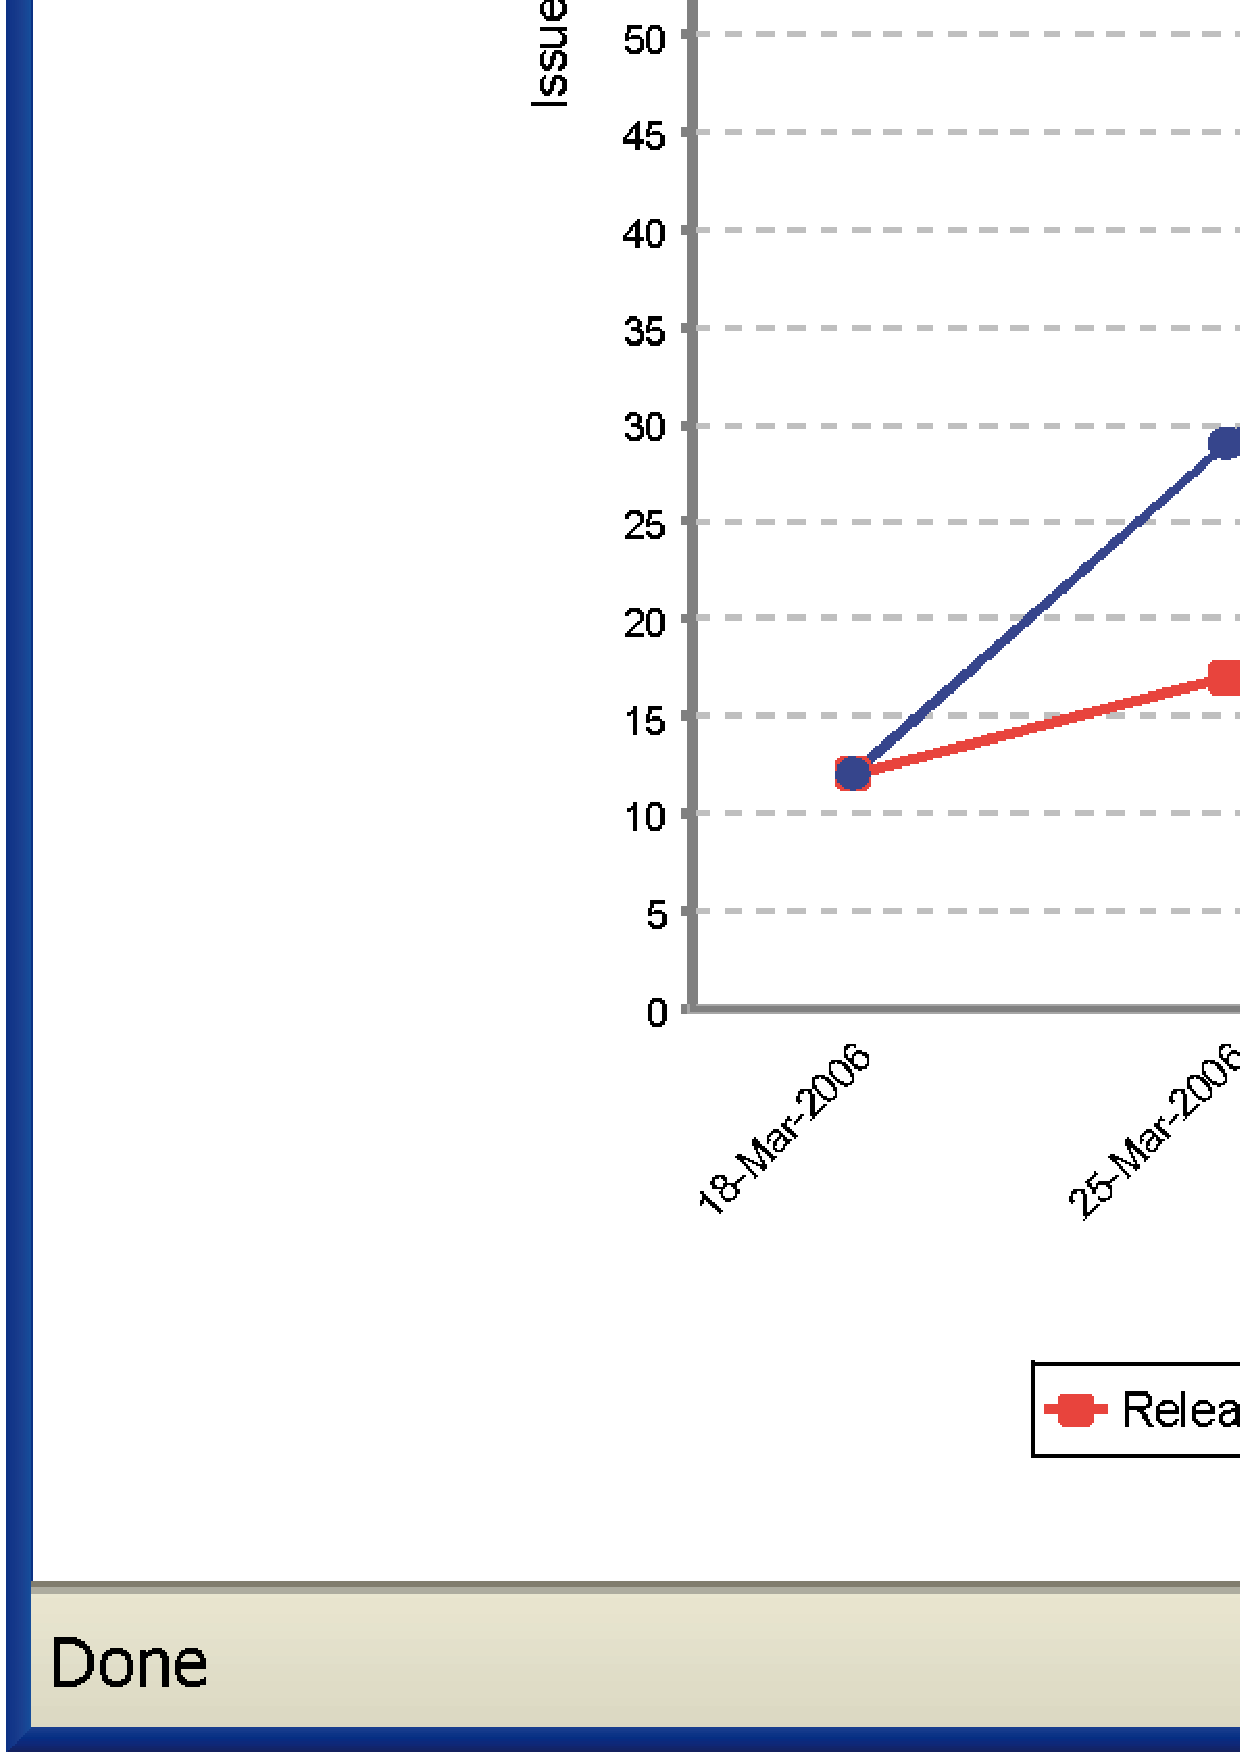
\includegraphics[height=0.90\textheight]{figures/ReleaseIssueTracking}
  \caption{Release Issue Tracking: Total vs. Open Issues} 
  \label{fig:ReleaseIssueTracking}
\end{figure}

An example of relatively high-level telemetry analysis is release cycle issue tracking. Figure \ref{fig:ReleaseIssueTracking} displays two issue tracking charts for ``Hackystat-7'' project release cycle 7.3 and 7.4 respectively. Each chart shows the total and remaining number of issues on the last day of each week during the two release cycles. The top blue line represents a telemetry stream for the total number of issues scheduled for that release; while the red line below represents a telemetry stream for the number of remaining issues. The release cycle is complete when the number of remaining issues touches zero. 
An interesting process level observation from the perspective of project management is that the manager did not schedule everything up-front. Instead, he added new issues almost every week. Nevertheless, he was able to manage the team to make consistent progress toward zero open issue to finish the release cycle. The red line (i.e., the bottom line) provided information about the trend in issue closure that helped the manager assess whether or not more issues could be added to that release cycle.
Another observation is that the telemetry charts in Figure \ref{fig:ReleaseIssueTracking} were generated when release cycle 7.4 was still in progress. By the end of May 6, 2006, there were still 11 open issues. From the perspective of project planning and scheduling, telemetry charts for previously finished release cycles, such as the chart on the top for release cycle 7.3, serve as the base line. By comparing the shape of telemetry streams in different release cycles, the project manager was able to make an in-process decision concerning whether the overall development process was stable, and estimate whether the team could finish the current release cycle on schedule.

Telemetry analysis can also be performed at a relatively low level to reveal details of software development process. An example of such an analysis is provided below, together with the introduction of basic telemetry language constructs: \textit{stream}, \textit{chart}, and \textit{report}. Figure \ref{fig:TelemetryReportChartStream} illustrates their relationship. 

\begin{figure}[p]
  \centering
  \includegraphics[height=0.90\textheight]{figures/TelemetryReportChartStream}
  \caption{Telemetry Report Analysis} 
  \label{fig:TelemetryReportChartStream}
\end{figure}

\clearpage
\subsubsection{Telemetry Report}

A telemetry report is a named set of telemetry charts that can be generated for a specified project over a specified time interval. The goal of a telemetry report is to discover how the trajectory of different process and product metrics might influence each other over time, and whether these influences change depending upon context.

For example, Figure \ref{fig:TelemetryReportChartStream} shows a telemetry report for ``Hacky2004-all'' project covering the time interval from the week of Feb 26, 2005 to the week of June 5, 2005. The report consists of two charts. Both charts show \textit{Unit Test Dynamics Telemetry}, which is an analysis of trends in the percentage of active time,\footnote{Active time is a proxy for developer effort and is based upon measuring the time spent writing and editing code inside an IDE.} allocated to testing (\textit{ActiveTime-Percentage}) the percentage of source code devoted to testing (\textit{JavaSLOC-Percentage}), and the percentage of test coverage that results from this effort and code (\textit{JavaCoverage-Percentage}). 

The two charts share the same time interval and project. The only difference is that they show unit test dynamics information for two different modules in the same project. Two developers are primarily responsible for the two modules respectively. Interestingly, the unit test dynamics telemetry trends for the two modules reveal a very different shape, indicating differences in the underlying approach to the development of the two modules. An important note is that software project telemetry does not presume any judgment as to which approach to development is better. Some projects might choose to trade a little testing for time-to-market. Others might require every single line of code perform exactly as intended.



\subsubsection{Telemetry Chart}

A telemetry chart is a named set of telemetry streams that can be generated for a specified project over a specified time interval. The goal of a telemetry chart is to display the trajectory over time of one or more process or product metrics.

For example, the same Figure \ref{fig:TelemetryReportChartStream} shows two instances of the same telemetry chart. Each chart contains three telemetry streams. You can see references to these three streams in the legend accompanying each chart. The legends also illustrate that telemetry streams can be parameterized: the top chart contains streams parameterized for the \textit{hackyZorro} module, while the bottom chart contains streams parameterized for the \textit{hackyCGQM} module.




\subsubsection{Telemetry Stream}

Telemetry streams are sequences of a single type of software process or product data for a single project over a specified time interval. They are best thought of as a kind of abstract data type representing one or more series of metric data values of the same type.

The time interval covered by a telemetry stream is divided into periods. The data points in each telemetry stream reflect the state of some key aspect of the software system under study during each period. The period can be relatively fine-grained such as \textit{daily}, or more coarse-grained such as \textit{weekly} or \textit{monthly}. Two types of information are typically represented by telemetry data points: 

\begin{itemize}
	\item Aggregated information --- The metrics values can be accumulated over the time period. Some examples are total coding effort, total lines added or deleted in the source code, total number of new bugs reported, etc.
	
	\item Snapshot information --- The metrics are only meaningful at a specific point in time. Some examples are the size of the source code, the number of open bugs, etc. Usually, the snapshot is taken at the beginning or at the end of each period.
\end{itemize}

For example, the time period used in the telemetry streams in Figure \ref{fig:TelemetryReportChartStream} is week. The data points in \textit{ActiveTime-Percentage} telemetry stream represent aggregated information. They are the total time spent on editing source code for the entire week. The data points in \textit{JavaSLOC-Percentage} and \textit{Coverage-Percentage} telemetry streams represent snapshot information. They are the number of source code lines and system test coverage at the end of each week. 

The advantage of telemetry is that it shows the history of some form of state in the project development environment, and helps the project manager detect changes in the development process. Another advantage is that it is generally tolerant of missing data. For example, there are missing dots in the telemetry streams in Figure \ref{fig:TelemetryReportChartStream}. While complete data provide the best support for project management or process improvement, occasional drop-outs of data should have little impact on the value of telemetry for decision-making. As a result, analyses built on top of telemetry streams can exhibit graceful degradation, providing value even when only partial data is available.




\subsubsection{Telemetry Language} \label{Intro:Solution:MetricsAnalysis:TelemetryLanguage}

Under the hood, telemetry reports, charts, and streams are generated using the telemetry language. The language serves two purposes:

\begin{itemize}
	\item Different software development environments and different projects might have different requirements for metrics analysis. The telemetry language provides a flexible mechanism that decouples the types of metrics we collect and the types of analyses we support.  
	\item Many interesting issues in software project management involve understanding the relationship between different metrics. For example, we might be interested in seeing whether an increased investment in code review pays off with less unit test failures, or increased test coverage, or less defects reported against the reviewed modules. The telemetry language enables interactive exploration of the relationship between metrics by allowing a user to experiment with the data to see what perspectives provides best insight into his/her particular situation.
\end{itemize}

The telemetry language that is used to generate the telemetry report in Figure \ref{fig:TelemetryReportChartStream} is listed below:


\begin{verbatim}
   streams ActiveTime-Percentage(filePattern1, filePattern2) = {
     "Active Time Percentage",
     
     ActiveTime(filePattern1, "false") 
     / ActiveTime(filePattern2, "false") 
     * 100
   };

   streams JavaCoverage-Percentage(filePattern) = {
     "Java Coverage Percentage",
     
     JavaCoverage("Percentage", filePattern, "method") 
   };
   
   streams JavaSLOC-Percentage(filePattern1, filePattern2) = {
     "Java SLOC Percentage",
     
     FileMetric("Java", "sourceLines", filePattern1)
     / FileMetric("Java", "sourceLines", filePattern2)
     * 100
   };

   y-axis yAxis(label) = {label};
   
   chart UnitTestDynamics-Chart(filePattern, testFilePattern) = {
     "Unit Test Dynamics Telemetry",
     
     (ActiveTime-Percentage(testFilePattern, filePattern), 
      yAxis("ActiveTime%")),
      
     (JavaCoverage-Percentage(filePattern), 
      yAxis("Coverage%")),
      
     (JavaSLOC-Percentage(testFilePattern, filePattern), 
      yAxis("SLOC%"))
   };

   report UnitTestDynamics-Hackystat-Report() = {
     "Unit Test Dynamics: Selected Hackystat Modules", 
     
     UnitTestDynamics-Chart("**/hackyZorro/**", 
                            "**/hackyZorro/**/Test*"),
     UnitTestDynamics-Chart("**/hackyCGQM/**", 
                            "**/hackyCGQM/**/Test*")
   };

   draw UnitTestDynamics-Hackystat-Report();
\end{verbatim}

Two features of the language are illustrated in the example above:
\begin{itemize}
	\item The telemetry language supports arithmetic operations. You can add, subtract, multiply, and divide two telemetry streams.
	
	\item The telemetry language supports parameterization. The two charts in the ``UnitTestDynamics-Hackystat-Report'' definition are the same except that they are passed two different parameter values representing two different modules in the project.
\end{itemize}


\begin{figure}[p]
  \centering
  
\includegraphics[height=0.90\textheight]{figures/TelemetryExpertAnalysis}
  \caption{Telemetry Expert Analysis} 
  \label{fig:TelemetryExpertAnalysis}
\end{figure}

Figure \ref{fig:TelemetryExpertAnalysis} shows the telemetry analysis expert interface. The telemetry charts generated are exactly the same as those in Figure \ref{fig:TelemetryReportChartStream}. The only difference is that this time we are using the telemetry language to interact with the system directly. Note, however, that the second chart is not shown in Figure \ref{fig:TelemetryExpertAnalysis} because of space constraint. The telemetry language specification in Appendix \ref{Chapter:TelemetryLanguageSpecification} contains more detailed information.







\subsection{Process Methodology}
\label{Intro:Solution:ProcessMethodology}


\begin{figure}[p]
  \centering
  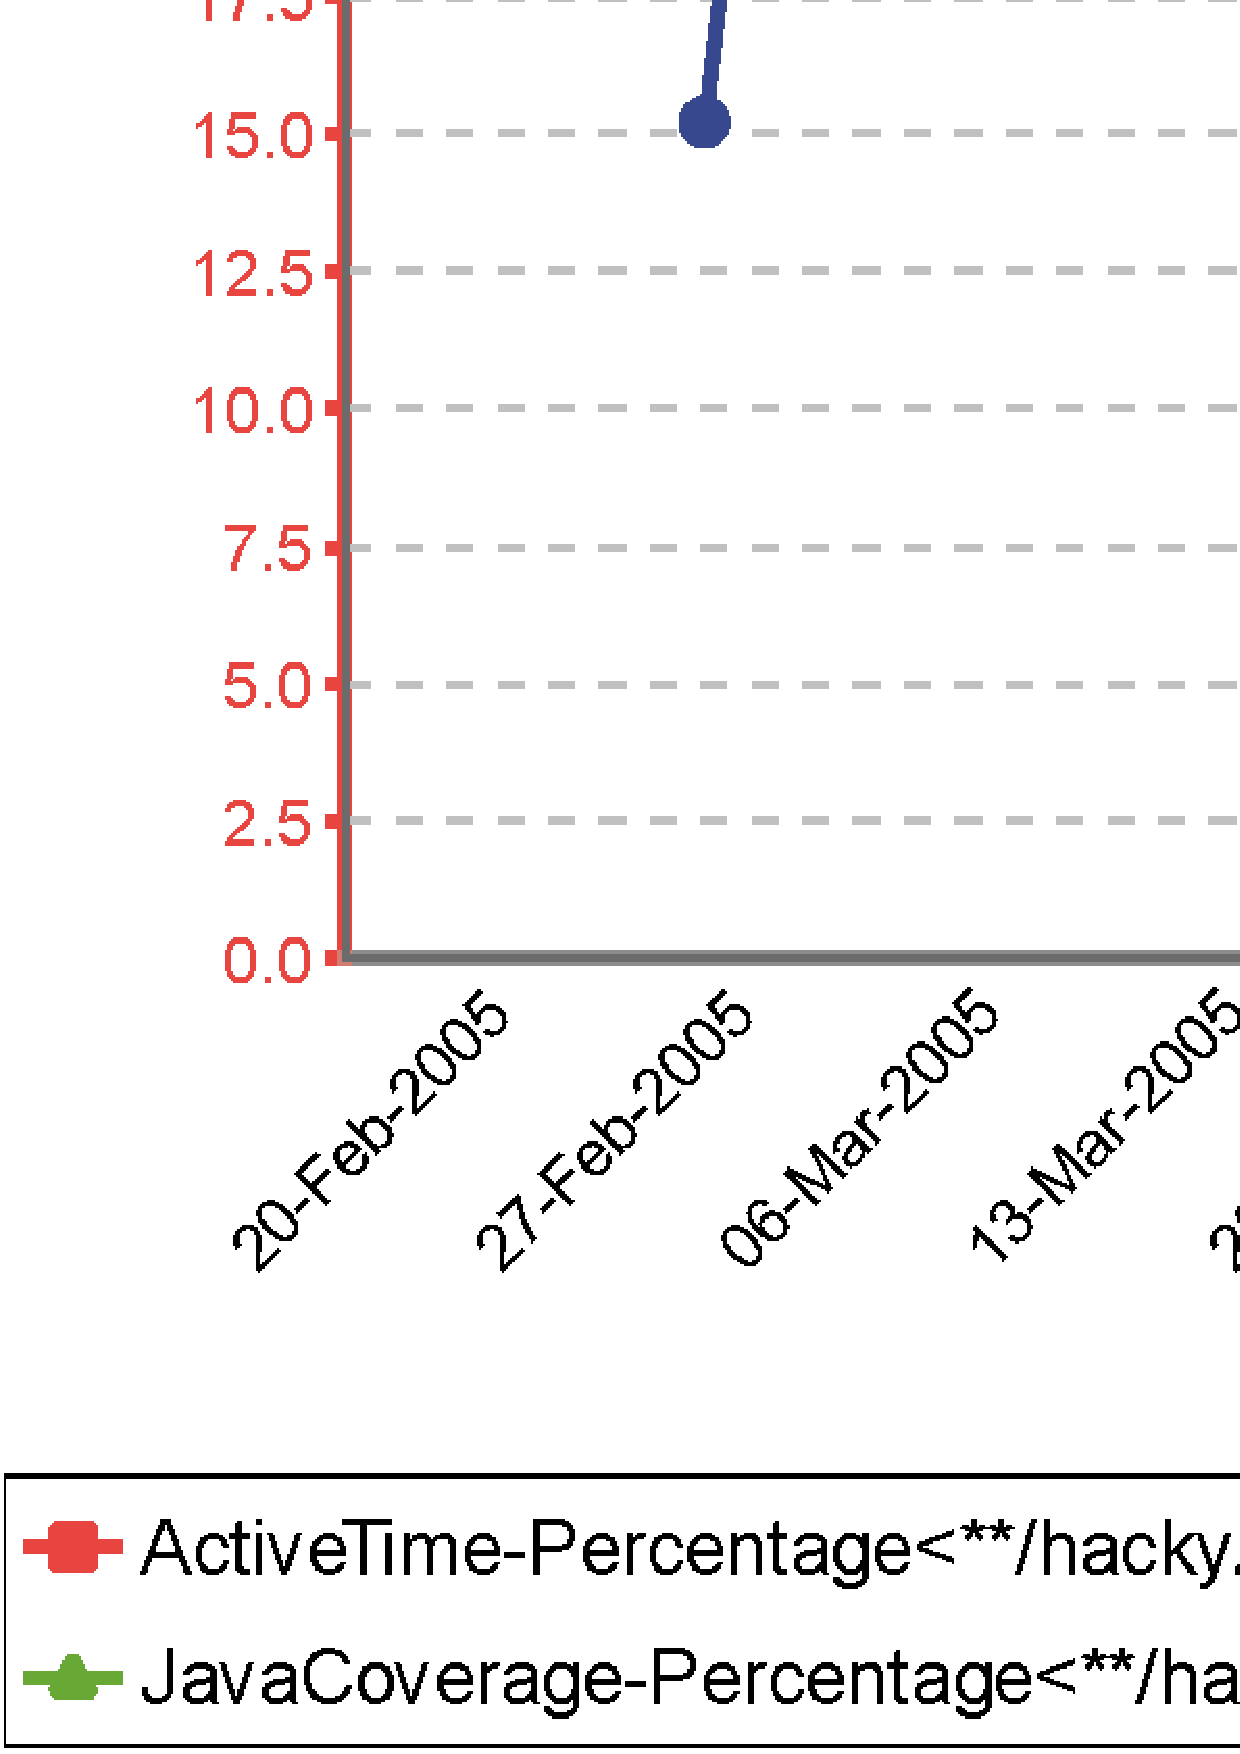
\includegraphics[width=1.00\textwidth]{figures/TelemetryChart}
  \caption{Telemetry Chart} 
  \label{fig:TelemetryChart}
\end{figure}

Figure \ref{fig:TelemetryChart} is an enlarged view of the top chart in Figure \ref{fig:TelemetryReportChartStream} and Figure \ref{fig:TelemetryExpertAnalysis}, showing unit test dynamics for the \textit{hackyZorro} module. 

A \textit{unit test} is a procedure used to verify that a particular module of source code is working correctly. This chart allows the comparison of the cost and the quality of unit testing. \textit{ActiveTime-Percentage} is the percentage of code-editing time allocated to writing test cases, and \textit{JavaSLOC-Percentage} is the percentage of source code lines that is unit test cases. Both of them are used as proxies for testing cost. \textit{JavaCoverage-Percentage} is the resulting test coverage (i.e., the percentage of the system exercised by test cases). It is used as a proxy for testing quality. Ideally, we wish to see high testing quality but low testing cost. When displayed in telemetry chart, we want to see the \textit{JavaCoverage-Percentage} telemetry stream near the top of the chart while the \textit{ActiveTime-Percentage} and \textit{JavaSLOC-Percentage} telemetry streams near the bottom of the chart. 

The telemetry chart in Figure \ref{fig:TelemetryChart} shows the development of the \textit{hackyZorro} module in the project. Both testing cost and testing quality were high at the beginning, but both were decreasing over time. After a little investigation, it turned out that the developer responsible for the module adopted \textit{test-driven development}\footnote{\textit{Test-driven development} is a programming technique emphasized in \textit{extreme programming} \cite{Beck:2000}. It requires writing test cases first before implementing the actual code.} methodology initially, but abandoned it during the development. This is very interesting. The telemetry streams in the chart clearly reveals the impact of the process-level changes\footnote{Again, the telemetry analysis does not presume any assumption that \textit{test-driven development} is better than other process methodologies. The judgment is left for the analysis user.}.

Telemetry streams consist of software process and product metrics. They are the basis of project management and process improvement. Telemetry charts and reports provide representation and display of telemetry trends. They make software developers more aware of their development processes by making them transparent and readily available. Telemetry streams for the same time interval are juxtaposed in the same telemetry chart or report to help developers detect covariance between different software metrics. For example, one might find that a drop in test coverage is frequently associated with an increase in the number of open bugs. This kind of information is important to project management, because it suggests a plausible causal relationship: low test coverage causes more bugs to slip through to the production stage. Based on this information, the project manager can implement changes to increase test coverage, and continue to use telemetry streams to monitor whether it indeed results in a decrease of the number of open bugs. At the same time, the project manager can monitor other telemetry streams, and check whether this corrective action has any unintended side effect to the development process. For example, he/she may wish to monitor productivity related telemetry streams to make sure that there is no reduction in developer productivity. The telemetry language provides a flexible mechanism decoupling the types of metrics and the types of analysis. It enables interactive exploration of the relationship between these different metrics. 

In general, applications of software project telemetry involve the following cycles to empirically guide the decision-making for project management and process improvement: 

\begin{enumerate}
  \item \textbf{Problem Detection} --- Use telemetry streams to monitor the development of a software project. Detect anomalies and undesirable trends in telemetry streams.
    
  \item \textbf{Process Improvement Hypothesis Generation} --- Determine plausible cause for the problem, and possible measure to correct it.
  
  \item \textbf{Process Change Implementation} --- Implement corrective measures.
  
  \item \textbf{Hypothesis Validation and Impact Analysis} --- Determine whether the problem goes away after corrective measures are implemented, and whether there are any unintended side effects caused by the corrective measures.

\end{enumerate}

The cycle continues until the project reaches completion.







%%%%%%%%%%%%%%%%%%%%%%%%%%%%%%%%%%%%%%%%%%%%%%%%%%%%%%%%%
%                                                       %
%                   S E C T I O N                       %
%                                                       %
%%%%%%%%%%%%%%%%%%%%%%%%%%%%%%%%%%%%%%%%%%%%%%%%%%%%%%%%%
\section{Thesis Statement}  \label{Intro:Thesis}

The claim of this thesis is that software project telemetry provides an effective approach to (1) automated metrics collection and analysis, and (2) in-process, empirically-guided software development process problem detection and diagnosis.

Compared to traditional model-base process prediction approaches, software project telemetry should be easier to use and cheaper to implement. It does not require software organizations to accumulate process and product metrics for finished projects in historical databases. Nor does it require expensive and error-prone model calibration before it can be used to make predictions. Instead, it focuses on evolutionary processes in development, and relies on metrics from an earlier stage of product development of the same project to make short-term predictions. For example, if system test coverage used to be almost 100\% but has been gradually dropping over time, then it may be a signal for management to re-allocate resources to improve project quality assurance. As a result, software project telemetry is best suited for in-process monitoring and control.

Software project telemetry should be robust. The information contained in telemetry streams should seldom be affected when there is occasional metrics drop out, and analyses should still provide decision-making value even if metrics collection starts midway through a project. 

Software project telemetry should also be flexible. There are no required set of metrics. Different software organizations can collect different sets of metrics according to their objectives, cost-benefit trade-offs, and measurement capabilities. For example, organizations with low process visibility can start with simple metrics such as source code size, and more metrics can be collected as their process matures and visibility increases.











%%%%%%%%%%%%%%%%%%%%%%%%%%%%%%%%%%%%%%%%%%%%%%%%%%%%%%%%%
%                                                       %
%                   S E C T I O N                       %
%                                                       %
%%%%%%%%%%%%%%%%%%%%%%%%%%%%%%%%%%%%%%%%%%%%%%%%%%%%%%%%%

\section{Empirical Evaluation}  \label{Intro:Evaluation}

The claim of this thesis was evaluated in two empirical studies: one in a classroom setting, and the other in the Collaborative Software Development Lab (CSDL). The primary goal was to assess metrics collection cost and decision-making value of software project telemetry. The secondary goal was to discover obstacles the developers might encounter during their use of the technology, and to gain insights about software project telemetry best practices and possible technology adoption barriers.
 
The classroom study was conducted in the two software engineering classes taught by Dr. Philip Johnson at the University of Hawaii in Spring 2005: one class for senior-level undergraduate students, and the other for introductory-level graduate students. By curriculum design, the students were divided into groups of 2 - 4 members collaborating on group projects and introduced to use software project telemetry to collect metrics and perform analyses on their own data. There were 25 students participating the study: 9 from the undergraduate session, and 16 from the graduate session.

The CSDL study was conducted in the Collaborative Software Development Lab at the University of Hawaii in Spring 2006, when a large scale software system (i.e., the Hackystat system itself) was being developed and maintained by a team of five on-site developers and a project manager. Three of the developers were Ph.D. students in software engineering (including me). They were hired by the lab working 20 hours a week. The other two were undergraduate students in their final semester. They were top students from the undergraduate software engineering class. They were working for the lab in exchange for personal development and course credit.

The two software development environments were quite different. In the classroom, there were a relatively large number of developers working on small scale class projects. In CSDL, there were a relatively small number of developers collaborating on a much larger project, which contained almost 300,000 lines of code and had been under development for five years. The CSDL developers had significantly more software engineering experience and process maturity compared to the average student in the classroom.

As a result, the two studies were structured differently. The classroom study was \textit{``passive''} in nature: though the students used software project telemetry to collect metrics and perform analyses on their own data, I did not make any deliberate attempts to help them improve their software development processes. On the other hand, the CSDL study was \textit{``active''} in nature: I introduced software project telemetry as a metrics-based process improvement program; I helped the project manager institute changes to improve project management practices; I also helped the developers gain insights into their development process.
Different data collection and analysis techniques were used in the two studies. 
The classroom study was relatively simple. My goal was to gather insights from a relatively large number of developers in a relatively short period of time. I distributed a questionnaire at the end of the semester to collect the student's opinions about software project telemetry. To increase my confidence in the validity of their self-reported opinions, I also analyzed their telemetry analysis invocation pattern to determine the extent to which their opinions were based on the actual system usage. 
In the CSDL study, I pursued a much more in-depth data collection and analysis strategy over a much longer period of time. I collected data from observations and interviews; I generated hypotheses from the data; I also tested the hypotheses in a limited way by making changes to the telemetry system or implementing new facilities to see whether the hypothesized outcome would come true or not.

The results of the two studies suggested that software project telemetry had acceptably-low metrics collection and analysis cost, and that it provided project management and process improvement decision-making values. 







%%%%%%%%%%%%%%%%%%%%%%%%%%%%%%%%%%%%%%%%%%%%%%%%%%%%%%%%%
%                                                       %
%                   S E C T I O N                       %
%                                                       %
%%%%%%%%%%%%%%%%%%%%%%%%%%%%%%%%%%%%%%%%%%%%%%%%%%%%%%%%%
\section{Contribution}  \label{Intro:Contribution}

There are three main contributions from this research:
\begin{enumerate}
	\item \textbf{The Concept of Software Project Telemetry}
	
In metrics collection, software project telemetry uses sensors to collect metrics automatically and unobtrusively. This sensor-based approach eliminates the chronic ``context-switch'' overhead inherent in manual approaches, such as PSP, and tool-assisted approaches, such as LEAP, PSP Studio, and Software Process Dashboard. 

In metrics decision-making, software project telemetry follows a light-weight approach by comparing telemetry trends in two different periods from the same project. The comparison involves a much smaller time scale than the whole project lifecycle. The metrics from the initial period of the project are used to establish a baseline and bootstrap the process. Project management and process improvement decisions are made by detecting changes in telemetry trends and comparing trends in two different periods in the same project. In-process control for a project that is still under development is made possible precisely because comparisons are made within a project. Since this approach does not involve the building of a statistical model in order to make cross-project comparison, it avoids many problems that typically exist in model-based approaches, such as spending the cost to accumulate a historical database of projects that may not be ``comparable'' to the current project. 

The two empirical studies I conducted showed that software project telemetry had sufficiently low metrics collection and analysis cost, and that it was able to deliver decision-making values, at least within the exploratory context of the two studies.

	
	\item \textbf{The Implementation of Software Project Telemetry}

Two pieces of software are the direct result of this thesis research. 
One of them is a server-side component, which includes the software code to interpret the telemetry language, the code to perform telemetry analyses and generate telemetry charts, and a web-based management console for telemetry construct definitions. The server-side component enables a user to log on to the server through a web browser to \textit{``actively''} explore relationships between different software metrics. 

The other is a client-side application that can be configured to automatically retrieve telemetry charts from the server and display them. It makes a sequence of telemetry charts continuously available to the user, providing \textit{``passive''} awareness of project status. 

The source code is GPL licensed, which encourages third-party improvement to be contributed back to the community. The system has already been adopted by several external sites, such as Sun Microsystem and the University of Maryland.

	
	\item \textbf{The Insights from the Empirical Studies}

Software project telemetry delivers best decision-making value when it can be customized to the specific needs of a software organization. The customization includes both setting up sensors to collect metrics and designing telemetry charts to perform analyses. ``Top-down telemetry design'' and ``bottom-up metrics collection'' are best practices. Top-down telemetry design refers to the idea that each telemetry chart should be designed with a clear purpose in mind, such as to help the development team meet a specific improvement goal. Bottom-up metrics collection refers to the recommendation to collect whatever metrics a software organization can. The rationale is the low cost associated with sensor-based metrics collection. Even if there is no apparent need for a metric today, it can still be used to establish a baseline for comparison tomorrow. 

Due to the automated nature of metrics collection in software project telemetry, broken sensors might not be noticed immediately. However, the empirical studies suggested that it would be possible to design special-purpose telemetry charts to help developers make quick assessments of whether the underlying sensors are sending data correctly or not. Therefore, another best practice for an organization is to deploy these special-purpose charts and assign a designated person to examine them.

One adoption barrier for this technology is concern about the level of privacy and confidentiality accorded to the data, especially with the effort-related personal process metrics. Though the current implementation has a mechanism to limit the kinds of data that could be accessed by people other than the owner, overcoming this issue seems largely dependent on what the data are used for in an organization. In other words, are the data used to improve development processes or to evaluate developers' performance? Lack of telemetry expertise within an organization might be another technology adoption barrier, since	software project telemetry will not likely deliver the best value if used straight ``out of the box'' and effective use, at least at this point, appears to require customization of the telemetry charts and reports.
	

\end{enumerate}







%%%%%%%%%%%%%%%%%%%%%%%%%%%%%%%%%%%%%%%%%%%%%%%%%%%%%%%%%
%                                                       %
%                   S E C T I O N                       %
%                                                       %
%%%%%%%%%%%%%%%%%%%%%%%%%%%%%%%%%%%%%%%%%%%%%%%%%%%%%%%%%
\section{Thesis Organization}  \label{Intro:Organization}

This thesis is organized into the following chapters:
\begin{itemize}
  \setlength{\itemsep}{0pt}
  \setlength{\parskip}{0pt}
  \item Chapter \ref{Chapter:Intro} is this chapter where the problem statement and proposed solution is described.
  
  \item Chapter \ref{Chapter:RelatedWork} relates the current research to the broader context of existing work.
  
  \item Chapter \ref{Chapter:Telemetry} describes software project telemetry in detail.
      
  \item Chapter \ref{Chapter:Implementation} describes the design details of an implementation of software project telemetry.

  \item Chapter \ref{Chapter:EvaluationStrategy} gives a brief review of research methods and discusses the evaluation strategies of software project telemetry.
  
  \item Chapter \ref{Chapter:EvaluationInClassroom} reports on a case study of software project telemetry in software engineering classes.
  
  \item Chapter \ref{Chapter:EvaluationInCSDL} reports on a case study of software project telemetry in the Collaborative Software Development Lab at University of Hawaii.

  \item Chapter \ref{Chapter:EvaluationConclusion} synthesizes the results from the two case studies to gain further insights.
  
  \item Chapter \ref{Chapter:Conclusion} provides final concluding remarks of this thesis research. 
\end{itemize}



  \chapter{Software Project Telemetry}
\label{Chapter:Telemetry}

Software project telemetry is a novel light-weight software measurement approach. It includes both (1) highly automated measurement machinery for metrics collection and analysis, and (2) a methodology for in-process, empirically-guided software development process problem detection and diagnosis. In this approach, sensors collect software metrics automatically and unobtrusively. Metrics are abstracted to telemetry streams, charts, and reports through a domain-specific language for the representation of telemetry trends for high-level perspectives on software development processes. 
Compared to traditional metrics-based approaches, which are based primarily on historical project databases and model-based comparison, software project telemetry emphasizes project dynamics and in-process control. The comparison in software project telemetry involves much smaller time scales. The idea is that comparison can be made between two different periods of the same project instead of between two different projects, and that the changes in the development process and their trends can be used as the basis for decision-making in project management and process improvement.

This chapter is organized into the following sections. 
Section \ref{Telemetry:Overview} gives an overview of software project telemetry and its essential characteristics.
Section \ref{Telemetry:Data} discusses sensor-based metrics collection. 
Section \ref{Telemetry:Component} discusses telemetry language and telemetry constructs such as stream, chart, and report.
Section \ref{Telemetry:Process} discusses the telemetry-based methodology for 
        project management and process improvement.
Section \ref{Telemetry:Conclusion} summarizes this chapter.





%%%%%%%%%%%%%%%%%%%%%%%%%%%%%%%%%%%%%%%%%%%%%%%%%%%%%%%%%
%                                                       %
%                   S E C T I O N                       %
%                                                       %
%%%%%%%%%%%%%%%%%%%%%%%%%%%%%%%%%%%%%%%%%%%%%%%%%%%%%%%%%

\section{Overview} 
\label{Telemetry:Overview}

Encyclopedia Britannica defines telemetry as ``highly automated communication process by which data are collected from instruments located at remote or inaccessible points and transmitted to receiving equipment for measurement, monitoring, display, and recording.'' Perhaps the highest profile user of telemetry is NASA, where telemetry has been used since 1965 to monitor space flights starting from the early Gemini missions to the modern Mars rovers. Telemetry data, collected by sensors attached to a space vehicle and its occupants, are used for many purposes, such as gaining better insight into mission status, detecting early signals of anomalies, and analyzing impacts of mission adjustments.

The same concept can be applied to software project management: software project telemetry is an automated process and product measurement approach. It is used to gain insight into software development processes, detect early signals of project failures, and analyze impact of project decisions. In this approach, sensors unobtrusively collect time-stamped software metrics, which are abstracted into telemetry streams, charts, and reports. Trends in telemetry streams serve as the basis for project management and process improvement. Telemetry charts and reports provide visualization. By detecting changes and covariance in trends of different metrics, software project telemetry enables a more incremental, visible, and experiential approach to project decision-making. It has the following essential characteristics:

\begin{enumerate}
  \item Software project telemetry data are collected automatically by sensors that unobtrusively monitor some form of state in the project development environment.  In other words, software developers are working in a ``remote or inaccessible location'' from the perspective of metrics collection activities. This contrasts with software metrics data that require human intervention or developer effort to collect, such as PSP/TSP metrics \cite{Humphrey:1995}.
  
  \item Software project telemetry data consist of a stream of time-stamped events, where the time-stamp is significant for analysis. Software project telemetry is thus focused on evolutionary process in software development.  This contrasts, for example, with COCOMO \cite{Cocomo:1981, Cocomo:2000}, where the time at which the calibration data are collected about the project is not significant.
  
  \item Software project telemetry data are continuously updated and immediately available to both developers and managers. Telemetry data are not hidden away in some obscure database guarded by the software quality improvement group. They are easily visible to all members of the project for interpretation. 

  \item Software project telemetry exhibits graceful degradation. While complete sensor data provide best support for project management, telemetry analyses still provide decision-making value even if there is occasional dropout of sensor data, or if data collection starts midway through a project.      
  
  \item Software project telemetry is used for in-process monitoring, control, and short-term prediction. Telemetry analyses provide representations of current project state and how it is changing at various time scales. The simultaneous display of multiple project state values and how they change over the same time periods allow opportunistic analyses --- the emergent knowledge that one state variable appears to co-vary with another in the context of the current project.
  
\end{enumerate}





%%%%%%%%%%%%%%%%%%%%%%%%%%%%%%%%%%%%%%%%%%%%%%%%%%%%%%%%%
%                                                       %
%                   S E C T I O N                       %
%                                                       %
%%%%%%%%%%%%%%%%%%%%%%%%%%%%%%%%%%%%%%%%%%%%%%%%%%%%%%%%%

\section{Sensor-based Data Collection}
\label{Telemetry:Data}

In software project telemetry, metrics are collected \textit{automatically} by sensors that \textit{unobtrusively} monitor some form of state in the project development environment. Sensors are pieces of software collecting both process and product metrics.

Software process metrics are the metrics that assist in monitoring and controlling the way software is produced. Sensors collecting process metrics are typically implemented in the form of plug-ins, which are attached to software development tools in order to continuously monitor and record their activities in the background. Some examples are listed below:

\begin{itemize}

	\item A plug-in for an IDE (integrated development environment) such as Visual Studio \cite{Software:VisualStudio}, and Eclipse \cite{Software:Eclipse}. It can record individual developer activities automatically and transparently, such as code editing effort, compilation attempts, and results, etc.

  \item A plug-in for a version control system, such as Clear Case \cite{Software:ClearCase}, CVS \cite{Software:CVS}, and SVN \cite{Software:SVN}. It can monitor code check-in and check-out activities, and compute \textit{diff} information between different revisions.
  
  \item A plug-in for a bug tracking or issue management system, such as Bugzilla \cite{Software:Bugzilla}, and Jira \cite{Software:Jira}. Whenever an issue is reported or its status is updated, the sensor can detect such activities and record the relevant information.
  
  \item A plug-in for an automated build system, such as Cruise Control \cite{Software:CruiseControl}. It can capture information related to build attempts and build results.

\end{itemize}


Software product metrics are the metrics that describe the properties of the software itself. Sensors collecting product metrics are typically implemented as analyzers for software artifacts. These analyzers usually need to be scheduled to run periodically in order to acquire the continual flow of metrics required by telemetry streams. To automate these tasks, one can use a \textit{Cron} job\footnote{\textit{Cron} is a \textit{Unix/Linux} program that enables users to execute commands or scripts automatically at a specified time or date. The \textit{Windows} equivalent is called \textit{Scheduled Tasks}.}, or run them as tasks in automated build system. Some examples are listed below:

\begin{itemize}

	\item An analyzer that parses program source code to compute size or complexity information.
	
	\item An analyzer that parses the output of existing tools, such as Clover \cite{Software:Clover}, and JBlanket \cite{Software:JBlanket}, and converts them to a data format that can be used by software project telemetry.

\end{itemize}

There are many other possibilities. One can even imagine an exotic sensor that retrieves project cost and payroll information from a company's accounting database, if extraction of such information is permitted by the company policy. The point is: no matter what the sensor does and regardless of its implementation details, a sensor-based approach collects metrics \textit{automatically} and \textit{unobtrusively} in order to keep data collection cost low, so that developers are not distracted from their primary tasks -- developing software products instead of capturing process and product metrics.

This sensor-based approach eliminates the chronic overhead in metrics collection. While setting up sensors might require some effort, once they are installed and configured, sensor data collection is automatic. This contrasts with traditional data collection techniques, such as the paper-and-pencil based approach used in PSP/TSP \cite{Humphrey:1995}, or the tool-supported approach used in LEAP \cite{Moore:1999}, PSP Studio \cite{PspStudio:1997}, and Software Process Dashboard \cite{PspDashboard:2000}. These approaches require constant human intervention or developer effort to collect metrics. Even in the case of the tool-supported approach, the developer still cannot escape the chronic overhead of constantly switching back and forth between doing work and telling the tool what work is being done \cite{Johnson:2001, Johnson:2003}.

The fact that chronic overhead is eliminated from sensor-based metrics collection not only reduces the technology adoption barrier, but also makes it feasible for software organizations to apply measurement to a wide range of development activities and products in order to get a comprehensive quantitative view of development processes.


Admittedly, the sensor-based approach does come with some restrictions:

\begin{itemize}
	
	\item A sensor must be developed for each type of tool we wish to monitor. This is a one-time cost. Once the sensor is developed, it can be used by different software development organizations for different projects. The Collaborative Software Development Lab has already developed a repository of over 25 sensors for commonly-used tools.

  \item Some metrics may not be amenable to automated data collection. An example is software development effort. While it is feasible to instrument an IDE to automatically get information such as how many hours a developer has spent on writing code, it is almost impossible to construct a sensor that knows how much total effort a developer has contributed to a project. For instance, two developers might be discussing the design of a system in the hallway. It is almost impossible to collect this type of effort in an automated way. It is still an open research question whether \textit{all} important metrics can be captured by sensors or not. However, this research takes a more pragmatic view: it is only concerned with whether sensors can collect \textit{sufficient} metrics so that software project telemetry has decision-making value for project management and process improvement. 
 
\end{itemize}






%%%%%%%%%%%%%%%%%%%%%%%%%%%%%%%%%%%%%%%%%%%%%%%%%%%%%%%%%
%                                                       %
%                   S E C T I O N                       %
%                                                       %
%%%%%%%%%%%%%%%%%%%%%%%%%%%%%%%%%%%%%%%%%%%%%%%%%%%%%%%%%

\section{Telemetry Language and Telemetry Constructs} 
\label{Telemetry:Component}

Many interesting issues in software project management involve understanding the relationship between different measures. For example, we might be interested in seeing whether an increased investment in code review pays off with less unit test failures, and/or increased coverage, and/or less defects reported against the reviewed modules. Such questions require comparing a set of metrics values over time. The telemetry language provides a mechanism that facilitates interactive exploration of relationships between metrics.
%so that developers and managers can ``play with the data'' to see what perspectives provide insight to their particular situation.
The language has the following syntax:

\begin{verbatim}
  streams <StreamName> (<ParameterList>) = {
    <DocumentationString>, 
    <Expresion>
  };
    
  y-axis <YAxisName> (<Parameter>) = {
    label, 'integer|double|auto', lowerBound, upperBound
  };
  
  chart  <ChartName>  (<ParameterList>) = {
    <ChartTitile>, 
    <StreamReferences>
  };
    
  report <ReportName> (<ParameterLilst>) = {
    <ReportTitle>, 
    <ChartReferences>
  };
\end{verbatim}


Note, however, that the above syntax is not written in a strict mathematical notation. The formal grammar of the language can be found in Appendix \ref{Chapter:TelemetryLanguageSpecification}: \textit{Software Project Telemetry Language Specification}. 
Chapter \ref{Chapter:Intro} contains a real-world example of the language in Section \ref{Intro:Solution:MetricsAnalysis:TelemetryLanguage}, and the resulting telemetry report in Figure \ref{fig:TelemetryReportChartStream}.


Telemetry \textit{reports}, \textit{charts}, and \textit{streams} are basic constructs of the language. The relationship between them is illustrated in Figure \ref{fig:TelemetryReportChartStream} and discussed in Section \ref{Intro:Solution:MetricsAnalysis}. 
In essence, a telemetry report is a named set of telemetry charts that can be generated for a specified project over a specified time interval. The goal of a telemetry report is to discover how the trajectory of different process and product metrics might influence each other over time, and whether these influences change depending upon context.
A telemetry chart is a named set of telemetry streams. The goal of a telemetry chart is to display the trajectory of one or more process or product metrics over time. The \textit{y-axis} construct is used to specify the vertical axis of a telemetry chart. Note, however, that a telemetry chart definition does not include the information about its horizontal axis, because such information can be automatically inferred from the time interval over which the telemetry analysis is performed. 
A telemetry stream is a sequence of a single type of software process or product metrics. 
%Telemetry streams are best thought of as a kind of abstract data type representing one or more series of metric values of a similar type.
 
The data collected by sensors are time-stamped, and the time stamp is always significant in telemetry style metrics analysis. There may not be a simple one-to-one correspondence between sensor data and the data points in telemetry streams. Sensor data usually represents very fine-grained low level software process or product details, while the data points in telemetry streams represent higher level perspectives on the software system or its development process. Typically, sensor data need to be filtered, combined, and aggregated to derive a telemetry data point. 
For example, suppose we want to construct a telemetry stream representing the number of open bugs for a software project on a monthly interval for the entire year 2005. In addition, suppose we are using Bugzilla \cite{Software:Bugzilla}, and whenever a bug is opened or closed, the Bugzilla sensor records information such as event time stamp, event type (bug open or bug close), bug id, severity, etc. In order to compute the number of open bugs for each month in 2005, the telemetry reducer needs to scan the entire bug event sensor data and combine them in order to compute values for the telemetry data points.  
  
Telemetry reducers takes sensor data as input and output a series of telemetry data points. They are the ``atomic'' building blocks for telemetry constructs at the user level. They serve as the link between sensor data and telemetry streams. They can be thought of as the fixed ``alphabet'' from which any number of telemetry streams can be created by a user. A reducer must be available in order to construct a \textit{``simple''} telemetry stream\footnote{Telemetry streams can also be generated by applying mathematical operations or telemetry functions to existing telemetry streams. These are called \textit{``compound''} telemetry streams as opposed to \textit{``simple''} telemetry streams.}. Some example of general classes of telemetry streams are:

\begin{itemize}
	\item \textbf{Development Telemetry} --- These are telemetry streams generated from data gathered by observing the behavior of software developers as reflected in their tool usage, such as the information about the files they edit, the time they spend using various tools, and the changes they make to project artifacts, the sequences of tool or command invocations, and so forth. Such metrics can be collected by attaching sensors to Integrated Development Environments (e.g., Visual Studio, Eclipse, Emacs), configuration management system (e.g., CVS \cite{Software:CVS}, Clear Case \cite{Software:ClearCase}), issue management systems(e.g., Bugzilla \cite{Software:Bugzilla}, Jira \cite{Software:Jira}), etc.
	
	\item \textbf{Build Telemetry} --- These are telemetry streams generated from data gathered by observing the results of tools invoked to compile, link, and test the system. Such metrics can be collected by attaching sensors to build tools (e.g., Make, Ant \cite{Software:Ant}, Cruise Control \cite{Software:CruiseControl}), testing tools(e.g., JUnit \cite{Software:JUnit}), size and complexity counters(e.g., LOCC \cite{Software:LOCC}), etc.
	
	\item \textbf{Execution Telemetry} --- These are telemetry streams generated from data gathered by observing the behavior of the system as it executes. Such metrics can be collected by sensors attached to the system runtime environment to gather its internal state data (e.g., heap size, occurrence of exceptions), or to load testing tools (e.g., JMeter \cite{Software:JMeter}) of the system to gather system performance data.
	
	\item \textbf{Usage Telemetry} --- These are telemetry streams generated from data gathered by observing the behavior of users as they interact with the system, such as the frequency, types, and sequences of command invocations during a given period of time in a given system.

\end{itemize}











%%%%%%%%%%%%%%%%%%%%%%%%%%%%%%%%%%%%%%%%%%%%%%%%%%%%%%%%%
%                                                       %
%                   S E C T I O N                       %
%                                                       %
%%%%%%%%%%%%%%%%%%%%%%%%%%%%%%%%%%%%%%%%%%%%%%%%%%%%%%%%%

\section{Telemetry-guided Project Management and Process Improvement} 
\label{Telemetry:Process}

The basic steps of telemetry-guided process improvement are illustrated in Figure \ref{fig:TelemetryBasedProcessImprovement}. It involves cycles of problem detection, process improvement hypothesis generation, process change implementation, hypothesis validation, and impact analysis.
Following Hetzel \cite{Hetzel:1993}, a software organization is recommended to collect a basic set of metrics, such as code size, test coverage, and build results, for every project at all time. This basic set of metrics generates a basic set of telemetry streams, which provide insights into the current software development practice and help establish a base line for the current process.

\begin{figure}[p]
  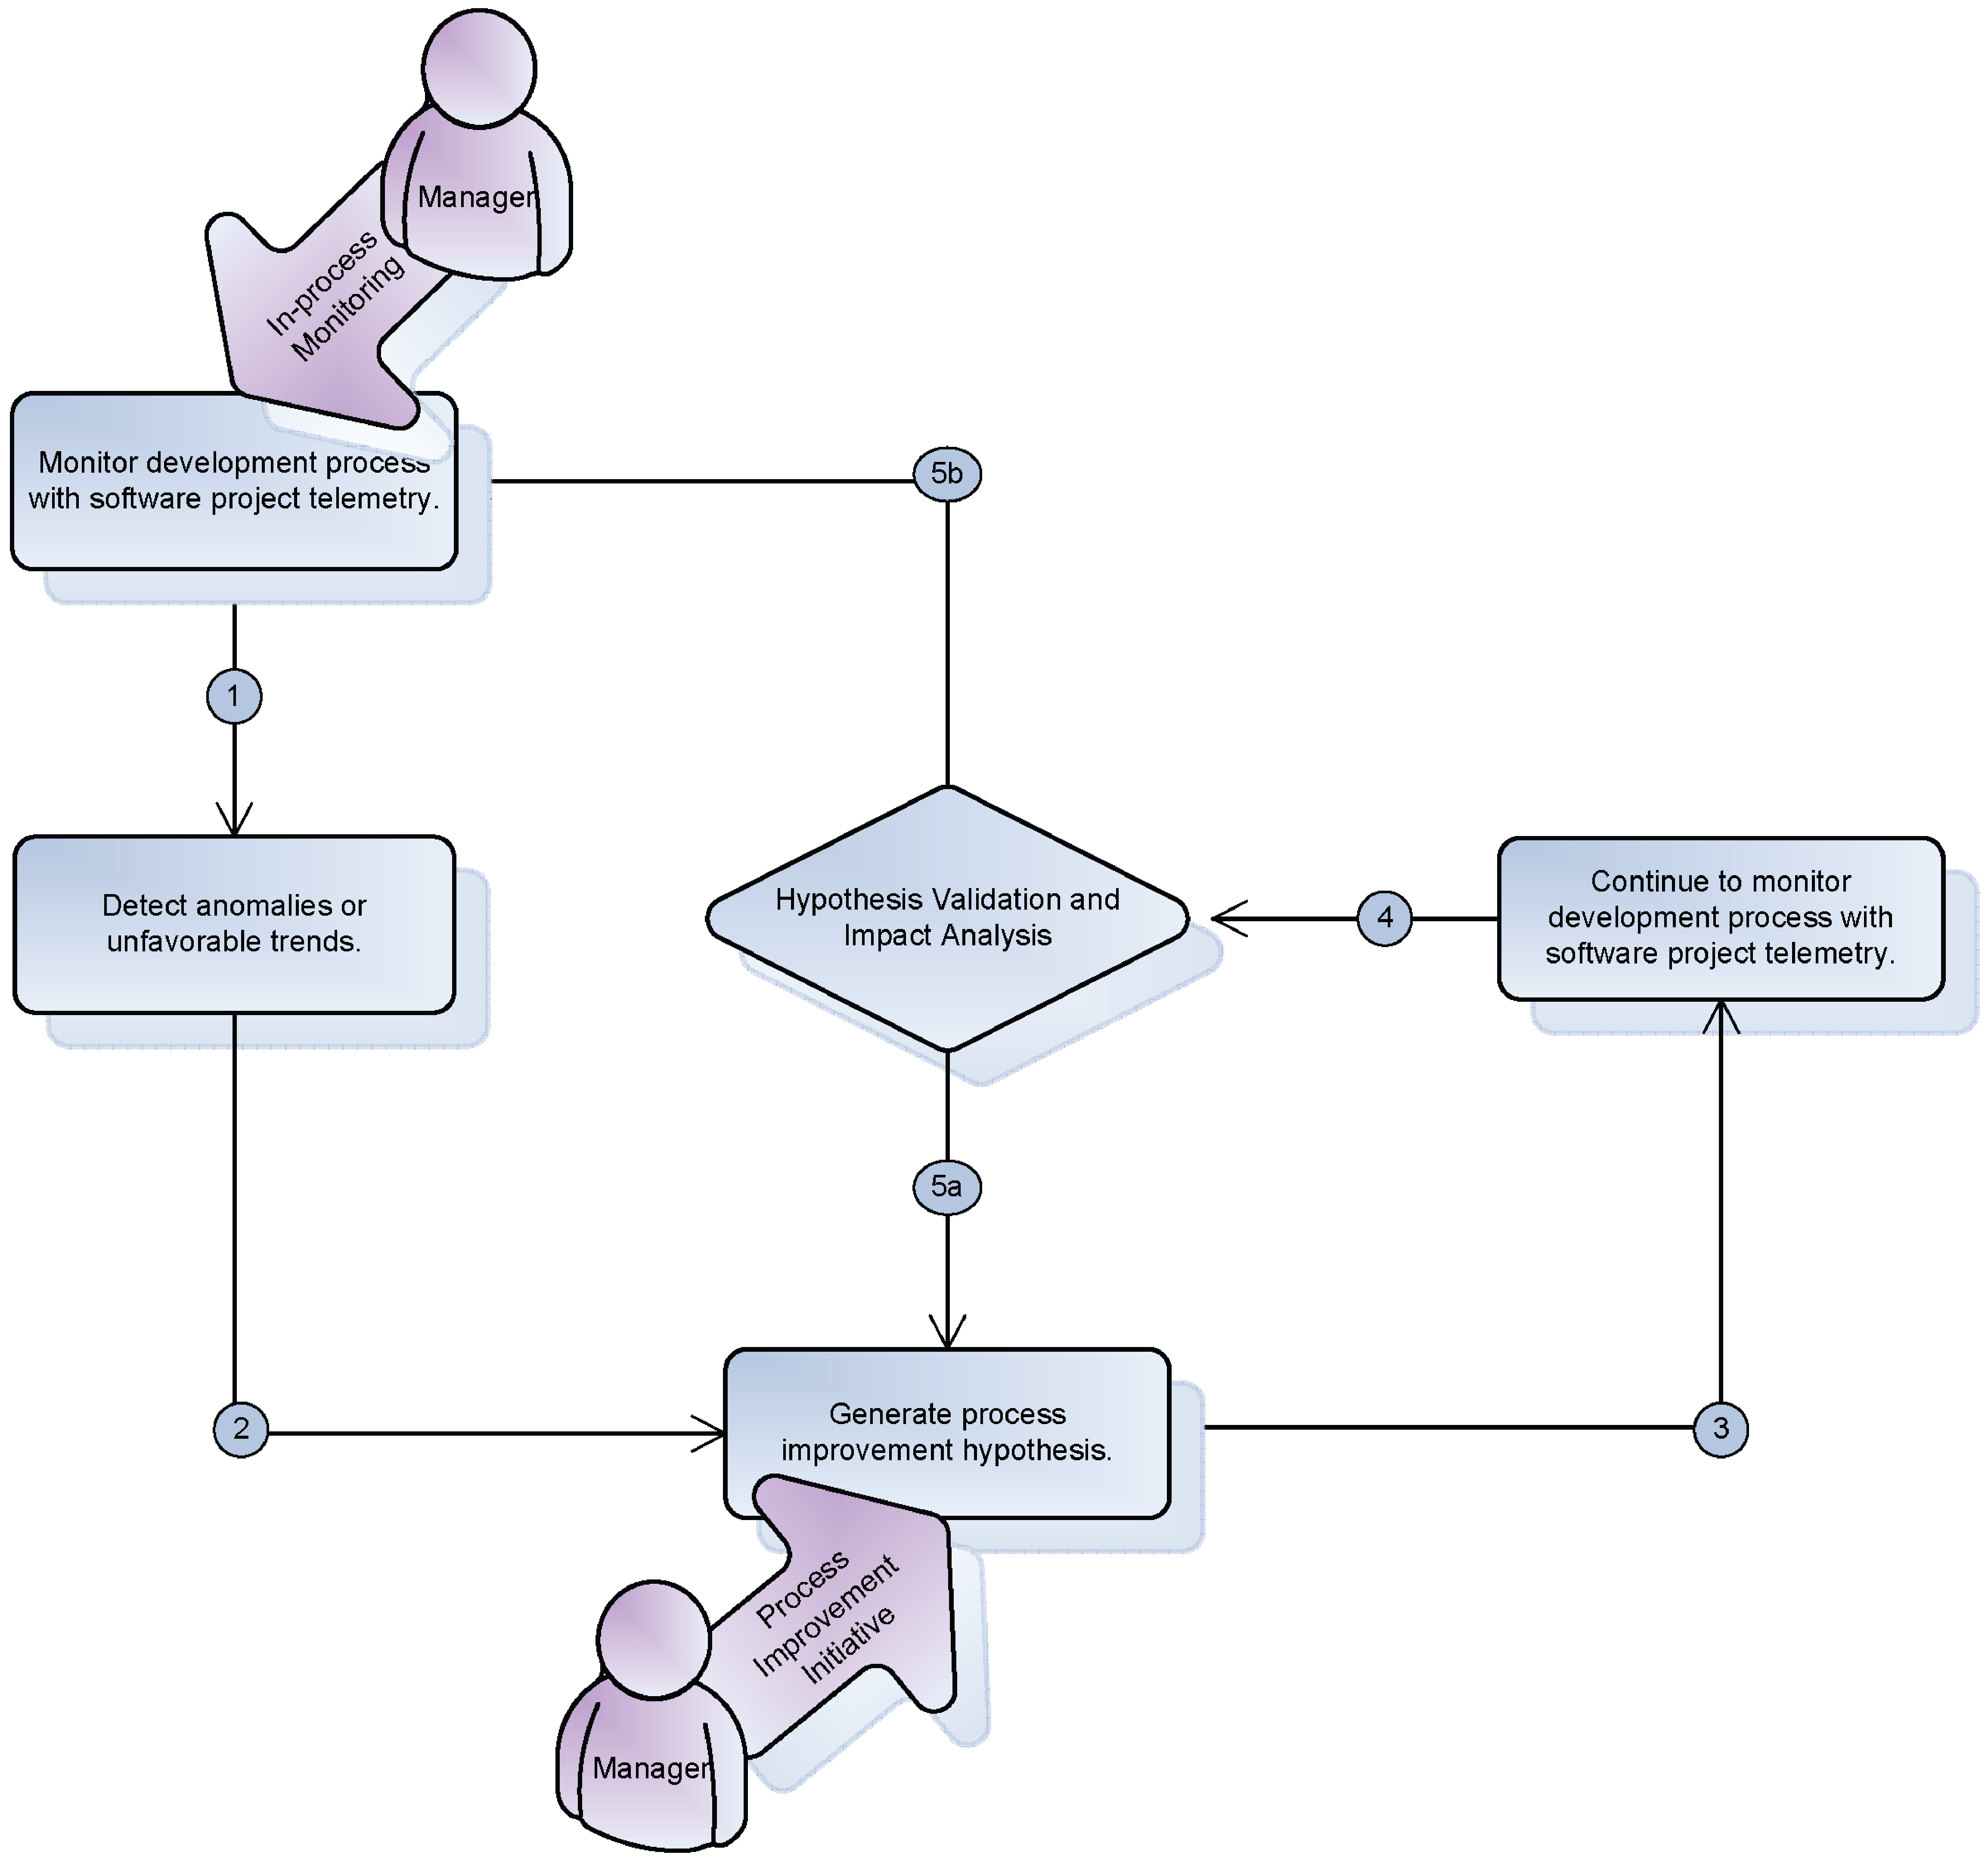
\includegraphics[width=1.00\textwidth]{figures/TelemetryProcess}
  \caption{Telemetry-based Process Improvement} 
  \label{fig:TelemetryBasedProcessImprovement}
\end{figure}


Software project telemetry can be used in two modes: (1) \textit{in-process project monitoring}, and (2) \textit{process improvement}. The two modes are closely related, and sometimes indistinguishable in practice. However, I will keep them separated in this discussion in order to make the concept clear. 

The steps for in-process project monitoring start from the upper arrow in Figure \ref{fig:TelemetryBasedProcessImprovement}. Telemetry streams are monitored for anomalies and unfavorable trends. If anomalies or unfavorable trends are detected, then the project manager must investigate the cause. Multiple telemetry streams, representing different perspectives on the development process, can be used to detect correlations. For example, the project manager might find that complexity telemetry values are increasing as well as defect density. Since telemetry streams consist of time-stamped events, the sequence of detected changes might help the project manager generate hypothesis about the causal relationship and corrective measures for process improvement. For example, the project manager might identify code complexity as a likely cause for high defect density. Once the process improvement hypothesis is generated, the project manager tries corrective actions such as simplifying over-complex modules, and continues to monitor telemetry streams in order to check whether the action results in a decrease in defect density. The project manager can also monitor other telemetry streams to check if such corrective action has unintended side-effects (impact analysis). If the hypothesis is correct, it will be validated by the newly-generated telemetry streams. If the telemetry streams indicate otherwise, then there must be other reasons that cause high defect density, and the project manager must try other corrective measures.

The steps for process improvement follow the same loop as the steps for in-process project monitoring. The only difference is that they start from the lower arrow in Figure \ref{fig:TelemetryBasedProcessImprovement}, and implementation of process improvement measures does  not have to wait until anomalies or unfavorable trends are detected in telemetry streams. 








%%%%%%%%%%%%%%%%%%%%%%%%%%%%%%%%%%%%%%%%%%%%%%%%%%%%%%%%%
%                                                       %
%                   S E C T I O N                       %
%                                                       %
%%%%%%%%%%%%%%%%%%%%%%%%%%%%%%%%%%%%%%%%%%%%%%%%%%%%%%%%%

\section{Chapter Summary}
\label{Telemetry:Conclusion}

In this chapter, I have described Software Project Telemetry in theory. It includes both (1) highly automated measurement machinery for metrics collection and analysis, and (2) a methodology for in-process, empirically-guided software development process problem detection and diagnosis. The next chapter introduces the tool implementation.


  \chapter{Related Work}
\label{Chapter:RelatedWork}

To understand how software project telemetry relates to other research, it is useful to think in terms of two concepts: \textit{measurement machinery} and \textit{process methodology}. Measurement machinery refers to how software metrics are collected and analyzed. In software project telemetry, sensors collect metrics automatically and unobtrusively. Metrics are abstracted into telemetry streams, charts, and reports, representing high-level perspectives on software development. Project management and process improvement decisions are based on the trends in telemetry streams. Process methodology refers to specific techniques used to improve the quality of software development effort. Software project telemetry employs cycles of process problem detection, improvement hypothesis generation, change implementation, and hypothesis validation to empirically guide project management and process improvement decision-making.

This chapter compares and contrasts software project telemetry to other metrics-based approaches. Some approaches, such as the Personal Software Process (PSP) \cite{Humphrey:1995, Humphrey:1996}, can be compared to software project telemetry with respect to both measurement machinery and process methodology. Other approaches, such as the Constructive Cost Model (COCOMO)  \cite{Cocomo:1981, Cocomo:2000}, are only comparable with respect to measurement machinery. Still others, such as the Goal-Quality-Metric paradigm (GQM) \cite{Basili:1988, Basili:1992}, and the Software Capability Maturity Model (CMM) \cite{Paulk:1993, SEI:1995}, are only comparable with respect to process methodology. 


This chapter proceeds with an overview of software measurement theory in Section \ref{RelatedWork:MeasurementOverview}, which serve as the foundation for any software measurement programs.
Section \ref{RelatedWork:PSP} discusses the Personal Software Process. 
Section \ref{RelatedWork:COCOMO} discusses process prediction models, especially the Constructive Cost Model. 
Section \ref{RelatedWork:GQM} discusses the Goal-Question-Metric paradigm.
Section \ref{RelatedWork:CMM} discusses maturity frameworks, especially the Software Capability Maturity Model.
Section \ref{RelatedWork:Summary} concludes the chapter with a summary.




%%%%%%%%%%%%%%%%%%%%%%%%%%%%%%%%%%%%%%%%%%%%%%%%%%%%%%%%%
%                                                       %
%                   S E C T I O N                       %
%                                                       %
%%%%%%%%%%%%%%%%%%%%%%%%%%%%%%%%%%%%%%%%%%%%%%%%%%%%%%%%%

\section{Software Measurement Theory}  \label{RelatedWork:MeasurementOverview}

As noted by DeMarco \cite{DeMarco:1982}: \textit{``You can neither predict nor control what you cannot measure.''} Measurement is the first step to transform software engineering from an art where the success of a project depends largely on the competence and commitment of individual developer, to a scientific discipline where project outcome is both predictable and controllable.

Measurement is defined as the process by which numbers or symbols are assigned to attributes of entities in the real world in such a way as to describe them according to clearly defined rules \cite{Fenton:1997}. This definition depends on two related concepts: entity and attribute. 
An entity can be a physical object such as a program, an event such as a release milestone, and an action such as testing software. In software measurement, entities are usually divided into two categories: software product and process. 
An attribute is a property of an entity, such as the size of a program, the size of test scripts, and the time required to finish a milestone. Attributes are generally divided into two categories: internal and external. Measures for internal attributes can be computed based on the entity itself; while measures for external attributes depend on both the entity and the environment in which the entity resides. 
The resulting classification scheme is depicted in Table \ref{table:Software-Measurement-Classification}. The cell for internal software process attributes is empty, because all software process metrics are dependent on the environment to various degrees.

\begin{table}[tbp]
	\centering
		\caption{Software Measurement Classification}
		\begin{tabular}{|p{0.30\textwidth}|p{0.30\textwidth}|p{0.30\textwidth}|} 
			\hline
			{} & \textbf{Internal Attributes} & \textbf{External Attributes} \\
			\hline
			\textbf{Software Product} & size, complexity, cohesion, coupling, etc. & quality, reliability, maintainability, portability, etc. %\cite{Musa:1987}
			\\
			\hline
			\textbf{Software Process} & {} & time, effort, cost, etc. \\
			\hline
		\end{tabular}
	\label{table:Software-Measurement-Classification}
\end{table}


The representation theory of measurement formalizes the process of mapping from an empirical relation system to a numerical relation system. A ``measure'' is nothing but the number assigned to describe some attribute of an entity by the mapping process. Not all mappings are the same. For example, the result of a sports competition, the first place, the second place, and the third place, are usually mapped to real numbers \textit{1}, \textit{2}, and \textit{3}, respectively. Since sports competition results contain only ordinal information, it is equally valid to use \textit{1}, \textit{10}, and \textit{100} as the mapping result. It is meaningless to add these numbers. This simple example shows that not all valid mathematical analyses in a numerical relation system are valid in the original empirical relation system.

Formally, the mapping, together with the associated empirical and numerical relation systems, is called the \textit{``measurement scale.''} It is the measurement scale that determines valid mathematical operations that can be performed. In general, measurement scales are classified into four categories with increasing level of restrictiveness: nominal, ordinal, interval, and ratio. More restrictiveness means more mathematical operators in the numerical relation system can be applied. Table \ref{table:MeasurementScaleAndOperator} lists the types of measurement scale and their corresponding valid mathematical operators.

\begin{table}[tbp]
	\centering
		\caption{Measurement Scale and Valid Mathematical Operations}
		\begin{tabular}{|p{0.45\textwidth}|p{0.45\textwidth}|} 
			\hline
			\textbf{Measurement Scale} & \textbf{Valid Mathematical Operators} \\
			\hline
			{Nominal Scale} & $=$ \\
			\hline
			{Ordinal Scale} & $=$ $>$ $<$ \\
			\hline
			{Interval Scale} & $=$ $>$ $<$ $+$ $-$ \\
			\hline
			{Ratio Scale} & $=$ $>$ $<$ $+$ $-$ $*$ $/$\\
			\hline
		\end{tabular}
	\label{table:MeasurementScaleAndOperator}
\end{table}

\begin{itemize}
	\item \textbf{Nominal Scale} --- The empirical relation system consists only of different classes. An example is the type of software fault, such as specification, design, and coding. There is no notion of ordering between different classes. As a result, any distinct number representation is a valid measure.
	
	\item \textbf{Ordinal Scale} --- It preserves ordering. The empirical relation system consists of classes that are ordered. An example is defect severity, such as minor, major, and critical. Any mapping that preserves the ordering is a valid mapping, and the numbers represent ranking only. Arithmetic operations, such as addition, subtraction, multiplication, and division, have no meaning.
	
	\item \textbf{Interval Scale} --- It preserves not only ordering but also differences. The difference between any two of the ordered classes in the range of the mapping is the same. Only addition and subtraction are valid. For example, when talking about time, we can say that ``year 2000 is 1000 years later than year 1000,'' and ``year 3000 is 1000 years later than year 2000,'' but we cannot say that ``year 2000 is twice as late as year 1000.'' 
	
	\item \textbf{Ratio Scale} --- It preserves ordering, differences, and ratios. The measurement starts from a zero element representing total lack of attribute, and increases at equal intervals known as units. All arithmetic operations, addition, subtraction, multiplication, and division, can be meaningfully applied. Using the length of software code as an example, we can say that ``this code contains no line,'' ``this code contains 20 more lines than that code,'' and ``this code contains twice as many lines as that code.''

\end{itemize}


 

In the current implementation of software project telemetry, mathematical computation of software metrics occurs at two consecutive stages: reduction processing and telemetry language processing. 

Reduction processing is the process of generating basic telemetry streams by filtering, synthesizing, and aggregating raw metrics collected by sensors. Telemetry reducers implement different reduction behaviors. They form the lowest level, atomic ``building blocks'' of the software project telemetry observable by an end user. Though data points in telemetry streams are mapped to real numbers by the reduction process, they can be of any measurement scale in theory. The reduction process itself is treated as a black box by the telemetry infrastructure. This is not a problem to end users, because the internal implementation details of telemetry reducers are not exposed to them. However, the developers who are responsible for reducer implementation must make sure that sensor data are manipulated in a meaningful way.

Telemetry language processing acts on telemetry streams. It includes telemetry function calls and telemetry arithmetic operations. The data points in telemetry streams are treated as if they were of ratio scale by the language interpreter. As a result, the language allows addition, subtraction, multiplication, and division between telemetry streams. This might cause a problem to a careless user, because there is the theoretical possibility of scale type mismatch. In other words, the telemetry language might allow meaningless mathematical operations to be applied to different types of metrics, such as adding code churn metric to unit test coverage metric. The problem could be solved by introducing a ``type'' system to the language, but doing so would significantly complicate the language design and its implementation. Currently, software project telemetry takes a pragmatic approach by relying on the user defining telemetry constructs to recognize nonsense operations. A topic for future research is to determine whether scale type mismatch is a significant problem in the use of software project telemetry, and to devise appropriate mechanisms to detect and/or prevent this problem.








%%%%%%%%%%%%%%%%%%%%%%%%%%%%%%%%%%%%%%%%%%%%%%%%%%%%%%%%%
%                                                       %
%                   S E C T I O N                       %
%                                                       %
%%%%%%%%%%%%%%%%%%%%%%%%%%%%%%%%%%%%%%%%%%%%%%%%%%%%%%%%%

\section{Personal Software Process}  \label{RelatedWork:PSP}

The Personal Software Process (PSP\footnote{Both Personal Software Process and PSP are registered service marks of Carnegie Mellon University.}) \cite{Humphrey:1995, Humphrey:1996} is a self-improvement process for software developers, and a ground-breaking approach that adapts organizational-level software measurement and analysis techniques to individuals. 

The PSP provides both measurement machinery and process methodology. The primary goal of the PSP is to improve project estimation and quality assurance. The goal is pursued by observation-evaluation-modification cycles. Developers observe their performance by recording how they develop software. They record the amount of time they spend, the size of the work product, and the defects they make while developing software. At the end of each project, developers evaluate how they performed by conducting standard analyses on the metrics they collected. Based on project postmortems, developers gain insight into their development process, and modify it in an attempt to improve it. A new cycle starts with the modified development process.

The original PSP proposed by Humphrey uses the very tedious manual approach to collect and analyze metrics. For instance, every time a compilation error occurs, the developer has to stop his/her current work, and log on paper forms the details of the error. Though several studies \cite{Ferguson:1997, Hayes:1997, Khajenoori:1995} have shown that the PSP appears to help improve software development, the anecdotal evidence suggests that the overhead involved in manual data collection affects its adoption. For example, a report on a workshop of PSP instructors \cite{Borstler:2002} reveals that in one course of 78 students, 72 of them abandoned the PSP because they felt \textit{``it would impose an excessively strict process on them and that the extra work would not pay off.''} None of the remaining 6 students reported any perceived process improvements. Moreover, manual data collection is susceptible to bias (either deliberate or unconscious), error, omission, and delay. A study \cite{Johnson:1998} of the data collected in the PSP showed that there were significant issues of data quality, and the combination of data collection and analysis errors called into question the accuracy of manual PSP results. Humphrey, the author of PSP, also admits in his book ``A Discipline for Software Engineering'' \cite{Humphrey:1995} that \textit{``it would be nice to have a tool to automatically gather the PSP data.''}

Tools, such as LEAP \cite{Moore:1999}, PSP Studio \cite{PspStudio:1997} and Software Process Dashboard \cite{PspDashboard:2000}, do exist to support the original manual PSP. These tools follow the same approach to user interaction by displaying dialog boxes where the user can log effort, size, and defect information. Though tool support lowers data collection overhead considerably, it turns out that the adoption of these tools is not satisfactory because of the requirement that the user constantly switch back and forth between doing work and telling the tool what work is being done \cite{Johnson:2001, Johnson:2003}. This chronic context switch appears to be a problem for many developers.

Software project telemetry uses sensors to collect metrics.\footnote{Sensor-based approach to metrics collection is pioneered in the Hackystat project \cite{Johnson:2003}, developed in the Collaborative Software Development Lab at University of Hawaii. I have been on the Hackystat development team since 2002 while doing software project telemetry research.} Sensors are attached to software development tools, which monitor some form of state change in the project development environment. Sensors collect metrics automatically and unobtrusively so that developers are not distracted from their primary tasks -- developing software products. Compared to manual and tool-based metrics collection, the sensor-based approach not only automates metrics collection in an unobtrusive manner, but also eliminates the chronic context-switch overhead. Details about sensor data collection, along with its restrictions, are discussed in Section \ref{Telemetry:Data}.

With respect to process methodology, the PSP uses observation-evaluation-modification cycles to improve software development process. One cycle corresponds to the life time of a project, and process improvement is based on comparison of different projects. This is essentially model-based cross-project comparison. The limitation is that it requires a historical database of finished projects. The PSP does not yield benefit unless such a database is accumulated first. For example, one of the practices of the PSP is to use statistical regression to predict project time based on planned project size, which requires a sufficient number of data points with respect to time and size of the past projects. Even if the accumulation of a historical project database is not a problem, the PSP user still must make sure that the context of the current project is consistent with the contexts of the finished projects in the project database. Otherwise, the prediction process is like comparing apples to oranges. The context consistency problem will be discussed in detail in Section \ref{RelatedWork:COCOMO}, since all model-based approaches face the same limitation.

Similar to the PSP, software project telemetry uses cycles to improve the software development process. The cycle includes process problem detection, hypothesis generation, change implementation, and hypothesis validation. The difference is that a software project telemetry cycle does not correspond to the life time of a project. It involves much smaller time scale, and a single project typically has many cycles. The idea is that comparisons can be made between two different periods of the same project instead of between two different projects, and that the changes in the development process and their trends can be used as the basis for decision-making in project management and process improvement. Since software project telemetry does not make model-based cross-project comparisons, there is neither a need to accumulate a historical project database, nor a necessity to ensure context consistency between different projects.







%%%%%%%%%%%%%%%%%%%%%%%%%%%%%%%%%%%%%%%%%%%%%%%%%%%%%%%%%
%                                                       %
%                   S E C T I O N                       %
%                                                       %
%%%%%%%%%%%%%%%%%%%%%%%%%%%%%%%%%%%%%%%%%%%%%%%%%%%%%%%%%

\section{Constructive Cost Model and Model-based Process Predictions} \label{RelatedWork:COCOMO}

The Constructive Cost Model (COCOMO) \cite{Cocomo:1981, Cocomo:2000} is a model for software project cost / effort estimation. It belongs to the branch of software engineering research called \textit{model-based process prediction}. This section begins with the more general topic of model-based process prediction before going into the details of the COCOMO.

The research in the area of model-based process prediction typically involves the following basic procedure: (1) collect a set of process and product metrics, such as size, effort, complexity, and defects, for a set of completed software projects, (2) generate a model to fit the observed data, (3) and claim that the model can be used to predict characteristics of future projects. For example, a model might predict that a future project of size \textit{S} will require \textit{E} person-months of effort; another model might predict that the future implementation of a module with complexity \textit{C} will be prone to defects with density \textit{D}. 

Model-based process prediction can be compared to software project telemetry with respect to measurement machinery. The difference is that prediction in software project telemetry does not require model building. Instead, it relies on changes in the development process and their trends to make short-term in-process predictions. The predictions made in software project telemetry and those made in model-based approaches tend to be of a different nature: model-based approaches tend to make end-point estimations (i.e., predictions for all phases of a software project as a whole), such as $X$ man-hours are needed to finish project $A$; while software project telemetry tends to make in-process predictions, such as the number of open bugs in system $B$ will continue to increase if system test coverage does not stop dropping.

Since model-based process prediction follows similar approaches in model building and process prediction, COCOMO is used to illustrate how they work in general. COCOMO is chosen because it is one of the most widely available and accepted models in the public domain.
%The Constructive Cost Model (COCOMO) \cite{Cocomo:1981, Cocomo:2000}
It is developed by Barry Boehm and his associates at University of Southern California.  The model estimates effort and schedule required to complete a software project. COCOMO 81 was the original model published in the book \textit{Software Engineering Economics} \cite{Cocomo:1981}. It offers three levels of model with increasing detail and accuracy: basic, intermediate, and detailed. COCOMO II \cite{Cocomo:2000} is an updated version of the original model to reflect the changes in software development practice. Like the first version, COCOMO II offers three levels: application composition, early design, and post-architecture, to explicitly model the fact that uncertainty of effort and schedule estimates decreases through software project life cycle. 

The post-architecture model is used to illustrate how COCOMO works. The estimation equations in the post-architectural model are:
  \begin{equation}
    PM = A * \prod_{i=1}^{17}EM_{i} * Size ^{(B + 0.01 * \sum_{i=1}^{5}SF_{i})}
  \end{equation}

  \begin{equation}
    TDEV = C * PM ^{(D + 0.002 * \sum_{i=1}^{5}SF_{i})}
  \end{equation}
where $PM$ is estimated effort in person-months. A person-month is the amount of time one person spends working on a software development project for one month. Note that this is in nominal terms, which does not take schedule compression or expansion into account.\footnote{COCOMO II offers an effort multiplier $SCED$, which can be used to adjust for the effect of schedule compression or expansion.} $Size$ is the primary input to the model. It is expressed in thousands of source lines of code (KSLOC). COCOMO II not only offers detailed rules on how to count lines of code, but also provides methods to convert other counting results, such as function points\footnote{A function point is a measure of program size independent of technology and programming language. The value of function point $FP$ is the product of unadjusted function point $UFP$ and technical correction factor $TCF$. Support for setting up function point analysis program is available from International Function Point User Group (http://www.ifpug.org).} \cite{Albrecht:1983} and object points \cite{Banker:1991, Banker:1994}, to lines of code. $TDEV$ is the amount of calendar time it will take to develop the software product. The average number of staff can be derived by dividing $TDEV$ from $PM$.

$A$, $B$, $C$, $D$, $SF_i$ and $EM_i$ are all constants in the model. $SF_i$ is called scale factor which influences effort exponentially. Scale factors are used to account for the relative economy or dis-economy of scale encountered for software projects of different sizes. $EM_i$ is called effort multiplier which influences effort multiplicatively. Effort multipliers are used to adjust for different product, project, platform and personnel factors in different software product development. Both effort multipliers and scale factors are defined by a set of rating levels: \textit{Very Low}, \textit{Low}, \textit{Nominal}, \textit{High}, \textit{etc}. 

Every few years, the COCOMO team updates the model by supplying new calibration values for the constants to reflect latest change in software production practice in industry. For example, the calibration values for the COCOMO II 2000 post-architecture model were obtained by calibrating the model to the actual parameters and effort values for the 161 projects in the COCOMO II database at that time. These values represent the software industry average. COCOMO recommends its users to calibrate $A$, $B$, $C$ and $D$ to their local development environment in order to increase prediction accuracy of the model.

COCOMO enjoys wide acceptance in both academia and industry. Various extensions have been developed since the publication of the original model. These extensions include COQUALMO (Constructive Quality Model) \cite{COQUALMO:1999}, COCOTS (Constructive COTS Model) \cite{COCOTS:2000}, and CORADMO (Constructive Rapid Application Development Model) \cite{CORADMO:2001}. Commercial implementations include Costar from Softstart Systems \cite{Software:Costar}, Cost Xpert from Cost Xpert Group Incorporated \cite{Software:CostXpert}, and Estimate Professional from Software Productivity Center Incorporated \cite{Software:EstimateProfessional}. 

The basic idea behind COCOMO and other process prediction models is ``cross-project comparison.'' Unfortunately, there are a number of difficulties in adopting this method in practice.

First, model-based process prediction assumes that the software organization has a relatively stable and repeatable development process. However, according to a Software Engineering Institute (SEI) survey of 542 software development organizations \cite{Peterson:1997}, 67\% of them are at CMM Level 1: the lowest maturity level. By definition, the software processes at level 1 are \textit{ad hoc} and sometimes \textit{chaotic}, and they change as work changes. As a result, it is generally impossible to make predictions for organizations at this level. In other words, two-thirds of software organizations are incapable of benefiting from model-based process predition techniques, such as COCOMO.

Second, the prediction power of these models is highly dependent on how well model calibration is performed. This can be thought of as a context consistency problem. In order to use the model, practitioners must confirm that the set of projects used to calibrate the model are similar to the project they wish to predict. Otherwise, they must recalibrate the model using the data in the organization's historical project database. This involves replicating the model-building method within the practitioner's organization, with the risk that the organization may have already changed and the context of the current project may differ from those in the historical project database, not to mention the practicality and cost of accumulating such a historical project database in the first place. 

Lastly, model-based process predictions are primarily designed to be used at a very early stage of a software project, or even before a project actually starts. Therefore, they tend to make end-point estimations (i.e., the prediction is made for all phases of the project as a whole). For example, COCOMO estimates that 586 person-months are required to develop a software with estimated size of 100 KSLOC.\footnote{Suppose all scale factors and effort multipliers take the rating of \textit{nominal}. Using COCOMO II 1997 calibration data, the estimation equation is $PM = 2.94 * Size ^ {1.15}$.} But when 300 person-months have been spent writing 60 KSLOC, the model does not give any indication whether the project will still be on-target or not. The project manager will know the answer after the entire project is finished, but by that time the information is irrelevant. To put it simply, end-point estimation is not very effective for in-process control.

Software project telemetry avoids the above-mentioned difficulties by shifting the focus of process prediction. It makes no attempt to build a cross-project comparison model in order to make a prediction before the project starts. Instead, it employs a more agile approach to compare software processes in different periods within the same project. It relies on changes in software development process and the trends of those changes to make short-term predictions for the purpose of in-process project management. 










%%%%%%%%%%%%%%%%%%%%%%%%%%%%%%%%%%%%%%%%%%%%%%%%%%%%%%%%%
%                                                       %
%                   S E C T I O N                       %
%                                                       %
%%%%%%%%%%%%%%%%%%%%%%%%%%%%%%%%%%%%%%%%%%%%%%%%%%%%%%%%%

\section{Goal-Question-Metric Paradigm} \label{RelatedWork:GQM}

The Goal-Question-Metric paradigm (GQM) \cite{Basili:1988, Basili:1992} provides a top-down, goal-oriented process methodology: software measurement is driven by high level goals. Usually the business goals of an organization are formed first, and then translated into improvement goals of software development, which, in turn, are translated into measurement goals. A metrics program is used to fulfill these measurement goals. Based on the measurement results, the organization can generate hypotheses and make decisions to reach the software development improvement goals, and, finally, the business goals.

GQM measurement goal is stated in 5 dimensions: \textit{study object}, \textit{purpose}, \textit{quality focus}, \textit{view point}, and \textit{environment}. A concrete example can be found in \cite{Solingen:1998, Solingen:1999}, in which the authors studied causes and effects of interruptions on software development work, and their measurement goal was:

\begin{quote}	
 \textit{Analyze} interrupts and their effects \textit{for the purpose of} understanding \textit{with respect to} impact on schedule and the cost-benefit of interrupts \textit{from the viewpoint of} project team \textit{in the context of} project $X$.
\end{quote}

GQM includes a top-down methodology that translates measurement goals into questions that need to be answered in order to reach them. Based on the questions, a set of relevant metrics can be identified and collected, which provide answers to the questions. The methodology can be best visualized as a tree-structured graph in Figure \ref{fig:gqm}.

\begin{figure}[tbp]
	\centering
		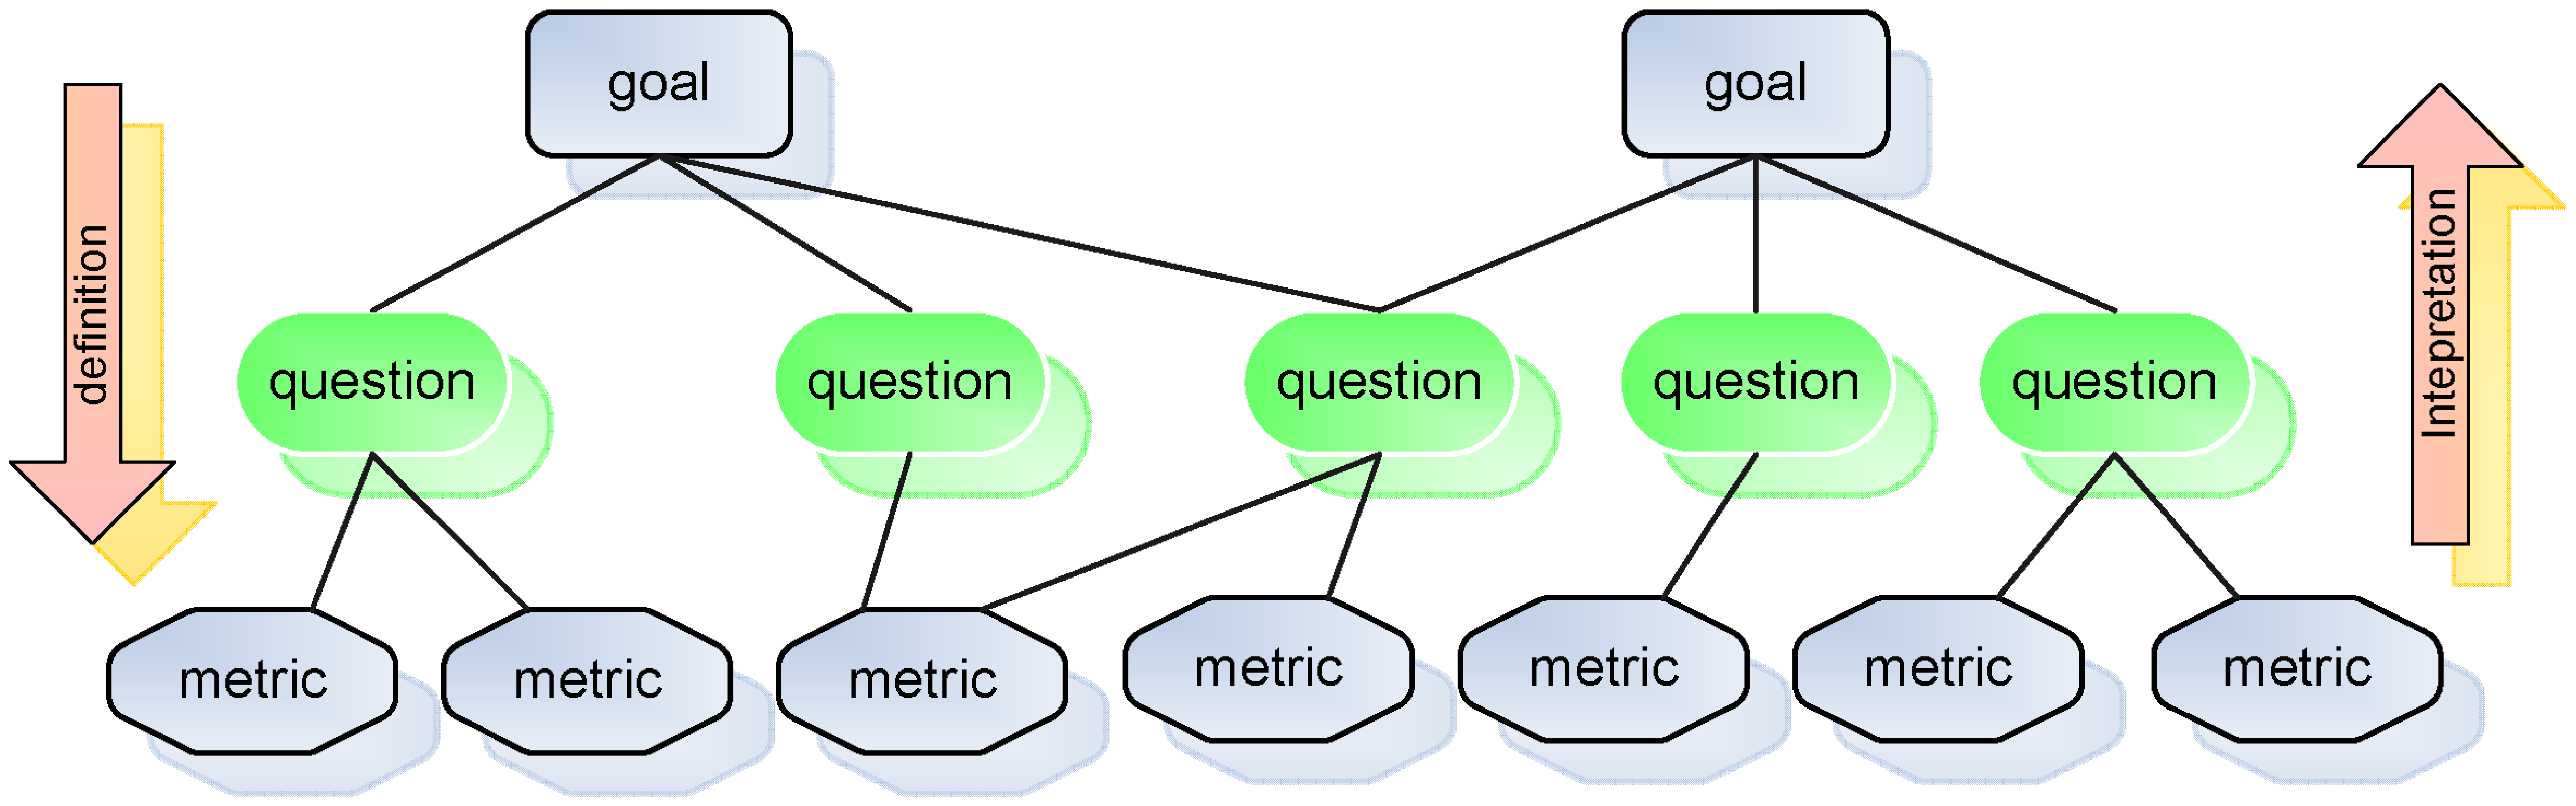
\includegraphics[width=1.00\textwidth]{figures/GQM}
		\caption{Goal-Question-Metric Paradigm}
	\label{fig:gqm}
\end{figure}

The GQM paradigm is well-known, and case studies of successful experience abound \cite{Basili:1996, Latum:1998, Fuggetta:1998}. The key to a success GQM implementation appears to be the establishment of well-defined measurement goals and the derivation of software metrics that can be used to provide useful information to meet the goals. However, the main criticism of GQM is the lack of attention to the actual measurement process: metrics collection and interpretation are not part of the paradigm. GQM implicitly assumes that once all required metrics are identified, the rest of the steps (metrics collection and interpretation) are easy.

Software project telemetry and the GQM paradigm can complement each other: GQM defines useful software metrics and relates them to an organization's business, project, product, and process goals; while software project telemetry provides an automated machinery for metrics collection and analysis. For example, ``Continuous GQM'' \cite{Lofi:2005} tries to implement GQM in an automated way in which data is collected, analyzed, and presented automatically with minimal human effort .








%%%%%%%%%%%%%%%%%%%%%%%%%%%%%%%%%%%%%%%%%%%%%%%%%%%%%%%%%
%                                                       %
%                   S E C T I O N                       %
%                                                       %
%%%%%%%%%%%%%%%%%%%%%%%%%%%%%%%%%%%%%%%%%%%%%%%%%%%%%%%%%

\section{Capability Maturity Model and Process Maturity Frameworks}  
\label{RelatedWork:CMM}

The Capability Maturity Model (CMM) \cite{Paulk:1993, SEI:1995} is a process maturity framework developed by the Software Engineering Institute (SEI). Other similar frameworks include ISO 9001 \cite{ISO9001:1987}, SPICE, and ISO/IEC 15504 \cite{ISO:1998, Eman:1998}. These frameworks share common properties, such as using metrics as a means to help software organizations improve their development process and to assess their capabilities. In these approaches, an externally defined reference framework is used to prescribe the activities, methodologies and practices a software organization should implement. The implicit assumption is that the prescribed processes are needed by most organizations in order to deliver high quality software in a repeatable and controllable manner, and a mature software development process will deliver high quality software products on time and within budget. Process assessment is used to compare organizational processes with the reference framework, which serves as an effective driver for process improvement. The assessment can be done by the software organization itself, by a second party, or by an independent third party. Based on the assessment results, organizations can find directions for process improvement.

Software project telemetry is closely related to process maturity. On the one hand, higher process maturity offers greater visibility into development activities. Since we can only measure what is visible in a process, higher process maturity means more telemetry streams can be generated and monitored. Process maturity frameworks offer a convenient context to plan software project telemetry program so that it grows to embrace additional aspects of software development and management. On the other hand, software project telemetry offers a methodology for process improvement based on quantitative feedback from existing development processes. It is especially helpful for software organizations to achieve high level process maturity where quantitative measurement is required.
Indeed, several authors have studied the relationship between software measurement and process maturity. For example, Table \ref{table:Maturity-Measurement} lists Pfleeger and McGowan's recommendation of collecting different measures depending on a software organization's CMM maturity level \cite{Pfleeger:1990}.

\begin{table}[tbp]
	\centering
		\caption{Process Maturity and Measurement}
		\begin{tabular}{|p{0.45\textwidth}|p{0.45\textwidth}|}
			\hline
			\textbf{CMM Maturity Level} & \textbf{What to Measure} \\
			\hline 
			\textit{Level 1 -- Initial: ad hoc} & baseline \\
			\hline 
			\textit{Level 2 -- Repeatable: process dependent on individual} & project \\
			\hline 
			\textit{Level 3 -- Defined: process defined and institutionalized} & product \\
			\hline 
			\textit{Level 4 -- Managed: process measured quantitatively} & process and feedback for control \\
			\hline 
			\textit{Level 5 -- Optimizing: continuing improvement based on measurement} & process and feedback for changing process \\
			\hline		
		\end{tabular}
	\label{table:Maturity-Measurement}
\end{table}

The following discussion uses CMM as an example to illustrate how a maturity framework works. Note that CMM is used here as a generic term referencing the works published by SEI, which include SW-CMM v1.0 (1991), SW-CMM v1.1 (1993), CMMI v1.02 (2000), and CMMI v1.1 (2002). CMMI \cite{Royce:2002} is the acronym for Capability Maturity Model Integration.

The goal of CMM is to determine whether a software development organization has a sound management infrastructure, and to assess its level of competence in building high quality software products. CMM is a staged model, which provides a set of requirements that software development organizations can use to set up software processes to control software product development. It ranks a software organization's process capability on a maturity level from 1 (lowest) to 5 (highest):

\begin{enumerate}
  \item \textbf{Initial Stage:} The software process at this level is characterized as \textit{ad hoc} and sometimes \textit{chaotic}. Success of software projects depends on the competence and commitment of individual developers. Few software processes are defined, and they change as work progresses. As a result, schedules, budgets and quality are generally unpredictable.
  \item \textbf{Repeatable Stage:} Basic project management processes are in place. Software organizations at this level have controls over software requirements, project planning and tracking, configuration management, quality assurance and subcontractor management. They are able to track project cost and schedule. They can repeat earlier successes on projects with similar applications.
  \item \textbf{Defined Stage:} The software processes for both management and engineering activities are documented, standardized and integrated into a standard software process for the whole organization. All projects use an approved, tailored version of the organization's standard software process to develop and maintain software.
  \item \textbf{Managed Stage:} Detailed measurement programs are in place to assess software development processes and product quality. Both software process and products are quantitatively understood and controlled. Software organizations at this level are able to tailor development processes to specific needs with predictable outcomes.
  \item \textbf{Optimizing Stage:} Continuous process improvement is enabled by quantitative feedback from software development processes and from piloting innovative ideas and technologies.
\end{enumerate}

Each maturity level is associated with a number of processes that an organization must implement. These processes are grouped into key process areas (KPA). Each KPA has a set of goals, capabilities, key practices, as well as measurements and verification practices. There are a total of 52 goals and 150 key practices. Some are related to setting up basic project management controls; some are aimed at establishing an infrastructure that institutionalizes effective software engineering and management processes across projects; while the rest are focused on performing a well-defined engineering process that integrates all software engineering activities to produce correct, consistent software products effectively and efficiently. The maturity level of a software organization is determined by its demonstrated capability in the key process areas associated with that level. Table \ref{table:CMM-KPA} lists CMM levels and their associated key process areas.

\begin{table}[tbp]
	\centering
		\caption{CMM Levels and Key Process Areas}
		\begin{tabular}{|p{0.25\textwidth}|p{0.65\textwidth}|} 
		  \hline
			\textbf{CMM Levels} & \textbf{Key Process Areas} \\
			\hline 
			\textit{Level 1 -- Initial} & None. \\
			\hline
			\textit{Level 2 -- Repeatable} & Requirements Management, Software Project Planning, Software Project Tracking and Oversight, Software Subcontract Management, Software Quality Assurance, Software Configuration Management. \\
			\hline
			\textit{Level 3 -- Defined} &  Organization Process Focus, Organization Process Definition, Training Program, Integrated Software Management, Software Product
Engineering, Intergroup Coordination, Peer Reviews. \\
			\hline
			\textit{Level 4 -- Managed} & Quantitative Process Management, Software Quality Management. \\
			\hline
			\textit{Level 5 -- Optimizing} & Defect Prevention, Technology Change Management, Process Change Management. \\
			\hline
		\end{tabular}
	\label{table:CMM-KPA}
\end{table}

CMM has received much attention in both academia and industry. Quite a few positive experiences have been reported in the literature \cite{Humphrey:1991, Dion:1993, Daskalantonakis:1994, Diaz:1997}. For example, Humphrey \textit{et. al. }\cite{Humphrey:1991} reported a software process improvement program at Hughes Aircraft with estimated annual saving at about \$2 million.

CMM makes use of software metrics to help software organizations improve their development process. It prescribes that in all key process areas measurement should be taken to determine the status of development activities. However, it does not prescribe how the measurement process itself should be implemented. In fact, Humphrey appears to be aware of the difficulty in implementing a measurement program in a software organization. He mentioned in \cite{SEI:1995} that:

\begin{quote}
\textit{``The greatest potential problem with the managed process is the cost of gathering data. There are an enormous number of potentially valuable measures of the software process, but such data is expensive to gather and to maintain.''}
\end{quote}
 
Software project telemetry can complement CMM. It provides not only an automatic and unobtrusive way of gathering software metrics data, but also a methodology of using quantitative data to analyze and modify software development process in order to prevent problems and improve efficiency. It is especially helpful for software organizations to achieve CMM Level 4 and 5.










%%%%%%%%%%%%%%%%%%%%%%%%%%%%%%%%%%%%%%%%%%%%%%%%%%%%%%%%%
%                                                       %
%                   S E C T I O N                       %
%                                                       %
%%%%%%%%%%%%%%%%%%%%%%%%%%%%%%%%%%%%%%%%%%%%%%%%%%%%%%%%%

\section{Chapter Summary}  \label{RelatedWork:Summary}

In this chapter, I have compared and contrasted Software Project Telemetry to other metrics-based approaches. The Personal Software Process suffers from chronic metrics collection and analysis overhead. The Constructive Cost Model relies on the assumption that software development process is stable and thus predictable. The Goal-Question-Metric paradigm offers a high-level abstract process methodology but lacks attention to the actual measurement process. The Capability Maturity Model prescribes that measurement should be taken to assess the status of development activities but does not specify how software measurement itself should be implemented. Software Project Telemetry addresses these limitations through automated metrics collection and analysis, and in-process, empirically-guided software development process problem detection and diagnosis. The next chapter gives a detailed discussion of Software Project Telemetry.


  \chapter{Implementation}  \label{Chapter:Implementation}

My implementation of software project telemetry has been integrated into the Hackystat system. Hackystat is an open-source framework developed in the Collaborative Software Development Lab (CSDL) at the University of Hawaii for automated collection and analysis of software product and process metrics and empirical software engineering experimentation. I have been contributing to its development since 2002. The relationship between my implementation of software project telemetry and Hackystat is illustrated in Figure \ref{fig:TelemetryImplementation}.
The implementation can be viewed as an extension to the Hackystat framework. CSDL members often use ``Hackystat'' as an umbrella term to refer to the framework plus all the extensions built on top of it. However, for the purpose of clarity, I will try to make a distinction between them. Throughout this chapter:

\begin{itemize}
	\item The \textit{``Hackystat framework''} refers to the core framework components that provide metrics storage service and extension plug-in mechanism.
	\item The \textit{``software project telemetry''} refers my implementation of software project telemetry.
	\item The \textit{``Hackystat system''} refers to the framework plus all the extensions built on top of it.
\end{itemize}

\begin{figure}[p]
  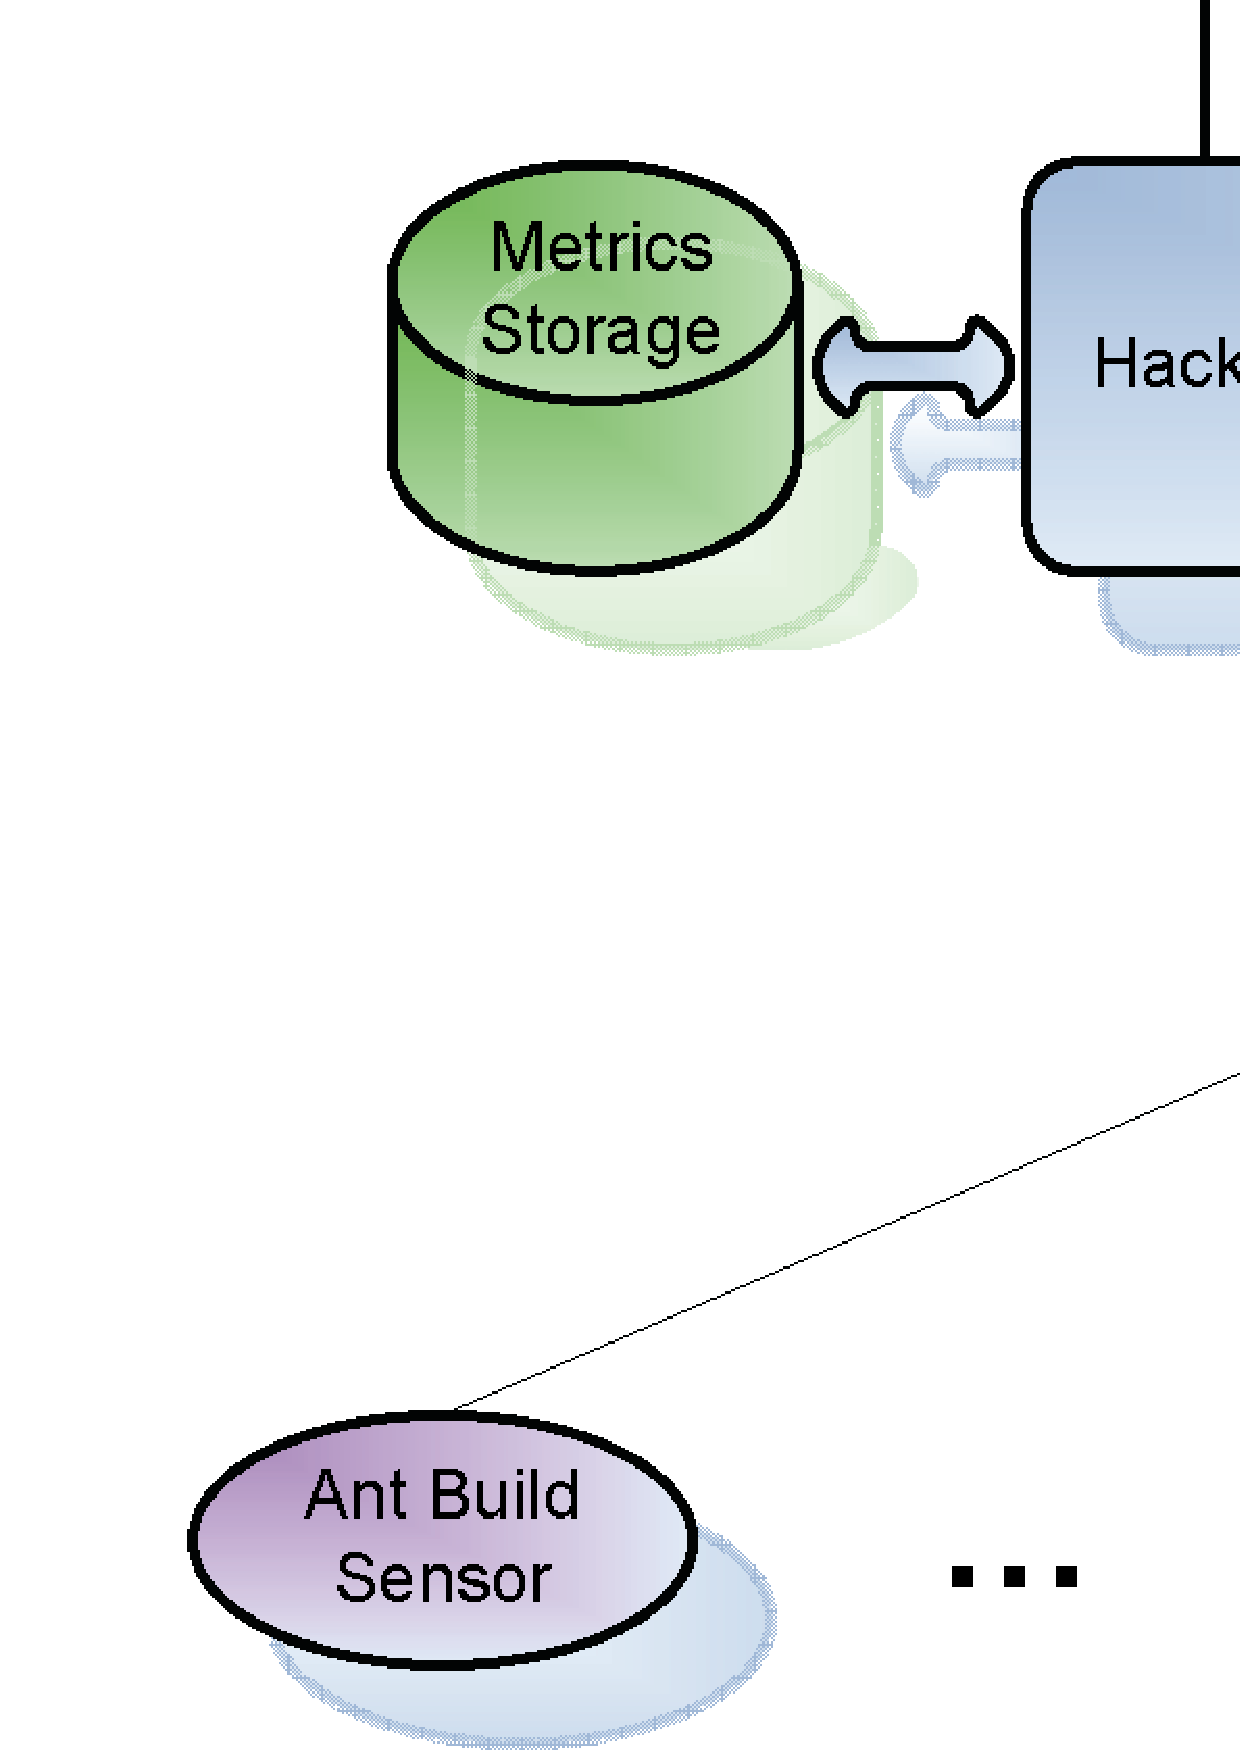
\includegraphics[width=1.00\textwidth]{figures/TelemetryImplementation}
  \caption{Software Project Telemetry System Implementation} 
  \label{fig:TelemetryImplementation}
\end{figure}

This chapter starts with a brief overview of the Hackystat framework and the services it provides in Section \ref{Implementation:Hackystat}. 
Section \ref{Implementation:Telemetry} describes my implementation of software project telemetry, which utilizes Hackystat framework services.
Section \ref{Implementation:ReducersFunctions} introduces all available telemetry \textit{reducers} and \textit{functions}.
Section \ref{Implementation:Summary} summarizes this chapter.







%%%%%%%%%%%%%%%%%%%%%%%%%%%%%%%%%%%%%%%%%%%%%%%%%%%%%%%%%
%                                                       %
%                   S E C T I O N                       %
%                                                       %
%%%%%%%%%%%%%%%%%%%%%%%%%%%%%%%%%%%%%%%%%%%%%%%%%%%%%%%%%

\section{Hackystat Framework} \label{Implementation:Hackystat}

Hackystat is an open-source framework developed in the Collaborative Software Development Lab (CSDL) at the University of Hawaii for automated collection and analysis of software product and process metrics and empirical software engineering experimentation. 
The framework itself is tool, environment, process, and application independent. It does not presume a specific operating system platform, a specific integrated development environment, a specific software process, or a specific application area. It is designed to be extended. Therefore, it only provides generic services such as metrics storage, project definition management, and an extension mechanism where new modules (functionalities) can be plugged in.

A Hackystat system is configured from a set of modules, which determine the actual functionality of the system: which development tools are supported, what types of software metrics are collected, and what analyses are run on the metrics. For example, several different research projects are being conducted using Hackystat. One research involves a Hackystat system configured from a set of modules specialized in low-level software process analysis \cite{Kou:2006}. Another research involves another Hackystat system configured from another set of modules trying to understand parallel software development for high performance computers \cite{Johnson:2005}. This thesis reports on my research involving yet another Hackystat system configured from yet another set of modules supporting project management and process improvement.




%%%%%%%%%%%%%%% S U B  S E C T I O N %%%%%%%%%%%%%%%%%%%%
\subsection{Metrics Storage}

The Hackystat framework exposes two interfaces related to metrics storage as illustrated in Figure \ref{fig:TelemetryImplementation}: one for metrics data reception, and the other for metrics retrieval.

The metrics data reception interface is used by sensors to send software process and product metrics. The communication occurs on an HTTP SOAP channel. Hackystat developers often refer to the Hackystat architecture as a client-server system. In this view, the \textit{``clients''} are development environment tools, such as editors (Emacs, Eclipse, Vim), configuration management systems (CVS, Harvest), build tools (Ant, Make), unit testing tools (JUnit), and so forth. For each of these tools, a custom sensor must be developed. The \textit{``server''} refers to the Hackytat framework kernel plus all the analysis extensions. They run inside a standard J2EE\footnote{J2EE stands for Java 2 Platform Enterprise Edition. Starting from version 5, Sun Microsystem has re-branded it as Java EE.} application container.

The metrics retrieval interface is used by metrics analysis extensions on the server side. Strictly speaking, the analysis code might opt not to use this interface directly. Instead, it may choose to rely on a higher level metrics abstraction mechanism which in turn depends on the metrics retrieval interface.

The Hackystat framework kernel handles metrics data storage automatically. The persistence engine is completely opaque, visible neither to the client-side sensors nor to the server-side analysis code. The current kernel implementation stores all metrics data in plain file system files in XML format. 



%%%%%%%%%%%%%%% S U B  S E C T I O N %%%%%%%%%%%%%%%%%%%%
\subsection{Project Definition Management} 

Sensors simply send bits of raw data concerning software process or product to the server. They know nothing about the larger context in which the development is performed. For example, during a typical day, a developer might work on several distinct tasks: an hour in the morning on requirements for an upcoming project, and two hours in the afternoon on maintenance fixes to an old system. For the requirements project, the developer is working in a team with one other person; while the system maintenance and development involves 12 people. In most cases, the developer will want to analyze the requirements data separately from the maintenance data. The developer will also probably want to gain a higher level perspective on the progress of the requirements project by combining his data and the relevant data from the other person he is working with. Similarly, it would be helpful to combine together the relevant data from all the 12 people working on maintenance to see how that project is progressing.
 
The Hackystat framework kernel supports team level analysis through project definitions. The project definition is designed to specify a context for analysis of sensor data, including the set of workspaces containing the artifacts associated with the project, the set of Hackystat users who are participating in the project and whose metrics should be combined together, and the time period during which the project is underway.




%%%%%%%%%%%%%%% S U B  S E C T I O N %%%%%%%%%%%%%%%%%%%%
\subsection{Extension Mechanism}

A Hackystat system provides all end user functionalities through extension modules. The framework exposes \textit{``extension points''} to support extensions along multiple dimensions including sensors, metrics types, metrics analysis, documentation, and so forth. For each new functionality, the framework requires the developer to specify a declaration file in XML format to supply information about the specific extension implemented. Detailed information about the extension points is available in the Hackystat developer documentation, which can be found at the Hackystat home page: \textit{www.hackystat.org}. 






%%%%%%%%%%%%%%%%%%%%%%%%%%%%%%%%%%%%%%%%%%%%%%%%%%%%%%%%%
%                                                       %
%                   S E C T I O N                       %
%                                                       %
%%%%%%%%%%%%%%%%%%%%%%%%%%%%%%%%%%%%%%%%%%%%%%%%%%%%%%%%%

\section{Hackystat Telemetry Module} \label{Implementation:Telemetry}

The core of my implementation of software project telemetry resides in a Hackystat extension module called \textit{``Core\_Telemetry''}. It contains about 15,000 lines of code. The module itself is extensible to accommodate new metrics types and analyses that might arise in the future. It exposes two extension points of its own, where custom implementation of \textit{telemetry reducers} and \textit{telemetry functions} can be plugged in. 

Just like the functionality of a Hackystat system is determined by its constituent modules, the functionality of the telemetry module hinges on the availability of reducers and functions. I have implemented over a dozen reducers and several functions to support this thesis research. They are distributed in the Hackystat modules where different types of software metrics are defined. They constitute about 13,000 lines of code. Available reducers and functions are listed in Section \ref{Implementation:ReducersFunctions}.



\subsection{Functional Description} \label{Implementation:Telemetry:FunctionalDescription}

The software project telemetry implementation provides three analyses where a user can perform telemetry related exploration. 

\begin{figure}[tbp]
  \includegraphics[width=1.00\textwidth]{figures/TelemetryDefinitionManagement}
  \caption{Telemetry Definition Management Console} 
  \label{fig:TelemetryDefinitionManagement}
\end{figure}

\begin{itemize}
	\item \textbf{Telemetry Expert Analysis} --- 
Figure \ref{fig:TelemetryExpertAnalysis} is a screenshot of the telemetry expert analysis. The user uses telemetry language to interact with the system directly to explore trends and relationships between different software product and process metrics. This is the most powerful and flexible analysis, and the user has the finest control.
%from determining which metrics to use and how to manipulate them, to the display details of the chart.
The expert analysis is especially useful when a user is experimenting with different forms of telemetry streams. Once the user is satisfied with the generated chart or report, he can create a persistent definition through the telemetry definition management console, so that later invocation of the same analysis can be performed through the telemetry chart/report analysis saving the effort of typing the definition again. Figure \ref{fig:TelemetryDefinitionManagement} is a screen shot showing a user creating a persistent definition of a telemetry chart with the definition management console.
	
	\item \textbf{Telemetry Report Analysis} --- 
Figure \ref{fig:TelemetryReportChartStream} is a screenshot of the telemetry report analysis.
This analysis performs the same analysis as the telemetry expert analysis, except that it hides the telemetry language from the end user. Instead of typing telemetry definitions directly, a user selects a predefined telemetry report from a drop-down list and performs the analysis.
The telemetry definition management console shown in Figure \ref{fig:TelemetryDefinitionManagement} allows a system administrator or a telemetry expert to define a set of commonly used telemetry charts and reports and made them available in the drop-down box that the end user sees.	This is a good way to lower the adoption barrier of software project telemetry, because it eliminates the need for a normal user to learn the telemetry language.
	
	\item \textbf{Telemetry Chart Analysis} ---
The telemetry chart analysis is similar to the telemetry report analysis. The only different is that the report analysis generates a group of related charts, while the chart analysis generates one single chart.

\end{itemize}








\subsection{Implementation Details}

The core of software project telemetry implementation resides in a Hackystat extension module called \textit{``Core\_Telemetry''}. The package structure is illustrated in Figure \ref{fig:TelemetryPackageStructure}. It includes the following components:

\begin{itemize}
	\item \textbf{Telemetry Language Parser} --- 
The telemetry language parser parses user input of telemetry definitions into an abstract syntax tree, which is a Java object representation of telemetry definitions. The formal grammar of the telemetry language is specified in Appendix \ref{Chapter:TelemetryLanguageSpecification}. Figure \ref{fig:TelemetryAST} is a UML diagram for static structure of the telemetry abstract syntax tree. Internally, the parser is generated using JavaCC \cite{Software:JavaCC}: a top-down Java parser generator.

	\item \textbf{Telemetry Streams Data Model} ---
This is the data model for telemetry streams. It contains computed values ready to be rendered or displayed to the end user.

	\item \textbf{Telemetry Reducers}\footnote{Telemetry reducers are also known as telemetry reduction functions, because the grammar to invoke a telemetry reducer is the same as the grammar to invoke a telemetry function. However, the similarity is superficial since the underlying implementation is completely different.} ---
This package contains the telemetry reducer extension point. A telemetry reducer aggregates low level software product and process data, and returns a collection of telemetry streams. To provide a custom implementation, a developer has to implement the \textit{``TelemetryReducer''} interface and supply a declaration file in XML format. The Core\_Telemetry module uses Java reflection to discover and load custom reducer implementations dynamically at runtime. 
	
	\item \textbf{Telemetry Functions}\footnote{This definition excludes telemetry reduction functions.} ---
This package contains the telemetry function extension point. A telemetry function takes a telemetry stream collection as input, and returns another telemetry streams collection as output. To provide a custom implementation, a developer has to implement the \textit{``TelemetryFunction''} interface and supply a declaration file in XML format. The Core\_Telemetry module uses Java reflection to discover and load custom function implementations dynamically at runtime. 
	
	\item \textbf{Telemetry Evaluation Engine} ---
The telemetry evaluation engine walks the telemetry abstract syntax tree, resolves references to telemetry definitions, and invokes telemetry reducers and functions. The evaluation result is either a telemetry chart or a telemetry report.
	
	\item \textbf{Telemetry Definition Management Console} ---
This package implements a web interface for the telemetry definition management console, which allows a user to manage persistent definitions of telemetry streams, charts, and reports. The persistent definitions are used by the telemetry chart/report analysis, so that a user can select from a list of predefined charts or reports to perform the analysis.

	\item \textbf{Telemetry Analysis} ---
This package implements the web UI for the three telemetry analyses introduced in Section \ref{Implementation:Telemetry:FunctionalDescription}: the expert analysis, the report analysis, and the chart analysis.
	
\end{itemize}



\begin{figure}[p]
  \includegraphics[width=1.00\textwidth]{figures/TelemetryPackageStructure}
  \caption{Core\_Telemetry Module Package Structure} 
  \label{fig:TelemetryPackageStructure}
\end{figure}


\begin{figure}[p]
  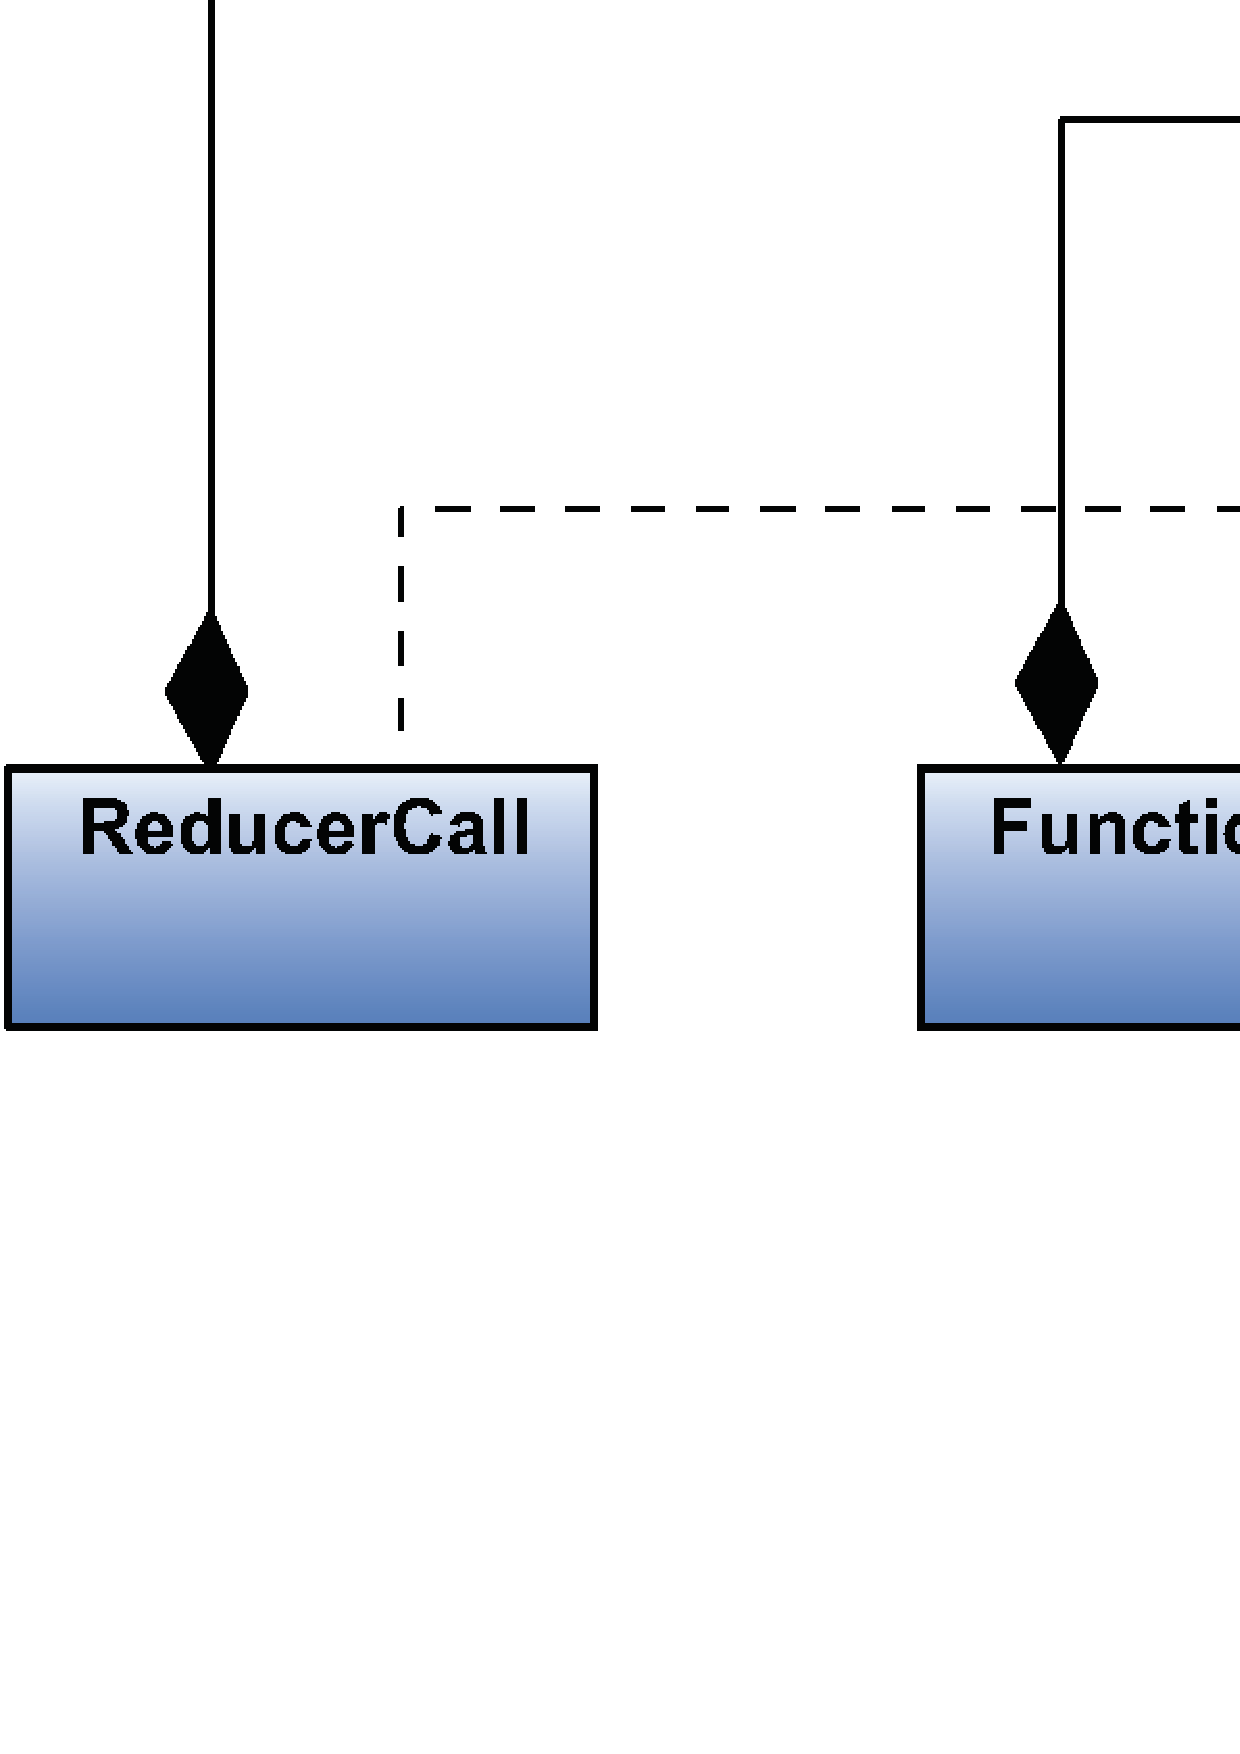
\includegraphics[angle=90, height=0.90\textheight]{figures/TelemetryAST}
  \caption{Telemetry Language Abstract Syntax Tree} 
  \label{fig:TelemetryAST}
\end{figure}










%%%%%%%%%%%%%%%%%%%%%%%%%%%%%%%%%%%%%%%%%%%%%%%%%%%%%%%%%
%                                                       %
%                   S E C T I O N                       %
%                                                       %
%%%%%%%%%%%%%%%%%%%%%%%%%%%%%%%%%%%%%%%%%%%%%%%%%%%%%%%%%
\newpage
\section{Telemetry Reducers and Functions} \label{Implementation:ReducersFunctions}

The Core\_Telemetry module is itself an extensible framework. It defines extension points for telemetry reducers and functions. The functionality of the telemetry module is determined by the available implementation of reducers and functions in a system. This section lists the reducers and functions that are currently available.







\subsection{Telemetry Reducers} \label{Implementation:Reducers}

The following telemetry reducers are available:

\begin{itemize}  
	\item \textbf{ActiveTime Reducer:}\\ 
Computes single telemetry stream for project active time in hours.
    
	\item \textbf{Build Reducer:}\\
Computes single telemetry stream for build success count or build failure count.

	\item \textbf{CodeChurn Reducer:}\\
Computes single telemetry stream for code churn: lines added or lines deleted.

	\item \textbf{CodeIssue Reducer:}\\
Computes single telemetry stream for the number of potential issues in the code generated by tools like FindBugs \cite{Software:FindBugs} and PMD \cite{Software:PMD}.

	\item \textbf{Commit Reducer:}\\
Computes single telemetry stream for code commit count.

	\item \textbf{CommitCycle Reducer:}\\
Computes single telemetry stream for the number of commits with specified local quality assurance behavior.

	\item \textbf{FileMetric Reducer:}\\
Computes single telemetry stream for source code size information.

	\item \textbf{IntegrationBuildFailure Reducer:}\\
Computes single telemetry stream for the number of integration build failures.

	\item \textbf{Issue Reducer:}\\
Computes single telemetry stream for the number of issues satisfying specified criteria.

	\item \textbf{JavaCoverage Reducer:}\\
Computes single telemetry stream for Java code unit test coverage.

	\item \textbf{JavaDependency Reducer:}\\
Computes single telemetry stream for Java code dependency.

	\item \textbf{LanguageFileMetric Reducer:}\\
Computes multiple telemetry streams for source code size information, one telemetry stream for each language found in the project.

	\item \textbf{MemberActiveTime Reducer:}\\
Computes multiple telemetry streams for member active time in hours, one telemetry stream for each member of the project.

	\item \textbf{MemberCodeChurn Reducer:}\\
Computes multiple telemetry streams for code churn, one telemetry stream for each member of the project.

	\item \textbf{MemberCommit Reducer:}\\
Computes multiple telemetry streams for code commit count, one telemetry stream for each member of the project.

	\item \textbf{MemberUnitTest Reducer:}\\
Computes multiple telemetry streams for the number of successful or failed unit test invocations, one telemetry stream for each member of the project.

	\item \textbf{Perf Reducer:}\\
Computes single or multiple telemetry streams for the values regarding a
performance test. Multiplicity is determined by reducer parameter values.

	\item \textbf{ReviewActivity Reducer:}\\
Computes single or multiple telemetry streams for project review active time in hours. Multiplicity is determined by reducer parameter values.

	\item \textbf{ReviewFile Reducer:}\\
Computes single or multiple telemetry streams for the number of files reviewed. Multiplicity is determined by reducer parameter values.

	\item \textbf{ReviewIssue Reducer:}\\
Computes single or multiple telemetry streams for the number of issues uncovered through code reviews. Multiplicity is determined by reducer parameter values.

	\item \textbf{UnitTest Reducer:}\\
Computes single telemetry stream for the number of successful or failed unit test invocations in the project.

	\item \textbf{WorkspaceActiveTime Reducer:}\\
Computes multiple telemetry streams for active time in hours in top level workspaces, one telemetry stream for each top level workspace.

	\item \textbf{WorkspaceCodeChurn Reducer:}\\
Computes multiple telemetry streams for code churn in top level workspaces, one telemetry stream for each top level workspace.

	\item \textbf{WorkspaceCommit Reducer:}\\
Computes multiple telemetry streams for code commit count in top level workspaces, one telemetry stream for each top level workspace.

	\item \textbf{WorkspaceCoverage Reducer:}\\
Computes single telemetry stream for Java code unit test coverage in top level workspaces, one telemetry stream for each top level workspace.

	\item \textbf{WorkspaceFileMetric Reducer:}\\
Computes multiple telemetry streams for source code size information in top level workspaces, one telemetry stream for each top level workspace.

\end{itemize}








\subsection{Telemetry Functions} \label{Implementation:Functions}

The following telemetry functions are available:

\begin{itemize}  
	\item \textbf{Add Function:}\\
Internal stock function supporting telemetry language operator ``+.''
	
	\item \textbf{Sub Function:}\\
Internal stock function supporting telemetry language operator ``-.''

	\item \textbf{Mul Function:}\\
Internal stock function supporting telemetry language operator ``*.''
	
	\item \textbf{Div Function:}\\
Internal stock function supporting telemetry language operator ``/.''

	\item \textbf{Filter Function:}\\
User callable function that filters out telemetry streams in a telemetry stream collection according to specified ranking function and threshold value.

	\item \textbf{FilterZero Function:}\\
Usable callable function that filters out telemetry streams with values of zero or no value in a telemetry stream collection.

\end{itemize}




%%%%%%%%%%%%%%%%%%%%%%%%%%%%%%%%%%%%%%%%%%%%%%%%%%%%%%%%%
%                                                       %
%                   S E C T I O N                       %
%                                                       %
%%%%%%%%%%%%%%%%%%%%%%%%%%%%%%%%%%%%%%%%%%%%%%%%%%%%%%%%%

\section{Chapter Summary} \label{Implementation:Summary}

In this chapter, I have introduced my implementation of software project telemetry. It is implemented as a Hackystat extension module. More detailed information and the source code are available at the Hackystat public website: \textit{www.hackystat.org}. The next chapter discusses the evaluation strategy for software project telemetry.


  
  \chapter{Evaluation Strategy}
\label{Chapter:EvaluationStrategy}


There are a variety of possible approaches to empirical evaluation of software project telemetry. This chapter provides an overview of these approaches based on \textit{Creswell's} book \textit{Research Design: Qualitative, Quantitative, and Mixed Methods Approaches} \cite{Creswell:2003}. The approach I chose is based on the concepts and techniques presented in that work.  
This chapter starts with a review of research methods in Section \ref{EvaluationStrategy:ResearchMethods}, followed by a discussion of the evaluation strategy with respect to software project telemetry in Section \ref{EvaluationStrategy:EvaluationStategy}.
Section \ref{EvaluationStrategy:Summary} concludes the chapter.



%%%%%%%%%%%%%%%%%%%%%%%%%%%%%%%%%%%%%%%%%%%%%%%%%%%%%%%%%
%                                                       %
%                   S E C T I O N                       %
%                                                       %
%%%%%%%%%%%%%%%%%%%%%%%%%%%%%%%%%%%%%%%%%%%%%%%%%%%%%%%%%

\section{Review of Research Methods} \label{EvaluationStrategy:ResearchMethods}

Creswell \cite{Creswell:2003} categorizes research methods into three paradigms: \textit{quantitative}, \textit{qualitative}, and \textit{mixed-methods}, according to their underlying philosophical assumptions about what constitutes knowledge and how knowledge is best acquired. The \textit{quantitative} paradigm is related to \textit{post-positivism}; the \textit{qualitative} paradigm is related to \textit{constructivism}; and the \textit{mix-methods} paradigm is related to \textit{pragmatism}.






\subsection{Quantitative Paradigm and Post-Positivism}

The philosophical underpinning of the quantitative paradigm is post-positivism. Post-positivism differs from positivism by recognizing that there is no absolute truth. Instead, it seeks to develop ``relevant true statements'' that can explain a situation and describe a causal relationship. Knowledge is conjectural in nature. The researcher tests a theory by specifying narrow hypotheses, collecting closed-ended data on predetermined instruments, and using statistical procedures to analyze the data to either support or refute the hypotheses. 

The most often used inquiry strategy in the post-positivist paradigm is the experiment. There are three basic experimental designs. From the least rigid to the most rigid, they are: correlation study, quasi-experiment, and true experiment. In a correlation study, a single group is studied without comparison to an equivalent non-treatment group. The quasi-experiment design introduces a control group, but it falls short on random assignment of study subjects.  The true experiment design employs both a control group and randomization. The purpose of increased rigidity is to control as many confounding variables as possible in order to determine true cause and effect. It is often thought that a true experiment is the only research method that can adequately measure the causal relationship. However, in the real world, a true experiment might be too expensive or might not be feasible at all.

The primary criteria with which to judge post-positivist research are \textit{internal validity} and \textit{external validity}. 
Internal validity is related to causality. It is demonstrated by showing that the cause not only correlates with but also precedes the effect, and that there is no plausible alternative explanation for the observed effect. 
External validity is related to generality. It is the degree to which the results obtained in a study can be applied to a larger population. 
Thus, for example, the use of control groups and randomization techniques are crucial to mitigate the threats to internal and external validity.








\subsection{Qualitative Paradigm and Constructivism}

The philosophical underpinning of the qualitative paradigm is constructivism. Constructivism assumes that all knowledge is ``constructed'' by observers who are the product of traditions, beliefs, and the social and political environment within which they operate. A researcher makes knowledge claims primarily based on constructivist perspectives, such as multiple meanings of individual experiences and socially or historically constructed meanings. The researcher tends to collect data through open-ended questions or by observing the participants' behaviors, trying to understand a particular situation, event, role, group, or interaction from their views. The research is largely an investigative process where the researcher gradually makes sense of a phenomenon by contrasting, comparing, replicating, cataloging, and classifying the objects of study \cite{Miles:1994}.

A major factor that distinguishes constructivism from post-positivism is that a researcher is not prescribing the questions that need to be answered from his / her own standpoint. Instead, the researcher tries to learn from the participants. In other words, the difference lies in the views about the nature of knowledge and how knowledge is best acquired. While hypotheses are specified \textit{a priori} in the post-positivist paradigm, they are established \textit{a posteriori} in the constructivist paradigm. Other unique characteristics of the constructivist paradigm are:

\begin{itemize}
	\item A constructivist study usually takes place in natural settings where human behavior and events occur.
	\item A constructivist study often uses multiple interactive methods such as open-ended questions, observations, and interviews.
	\item A constructivist study focuses on the participants' perceptions, experiences, and their understanding of the world in which they live and work.
	\item A constructivist study is emergent rather than tightly pre-configured. 
	\item A constructivist study places little importance on developing statistically valid samples, or on searching for statistical support for hypotheses.
\end{itemize}

A primary reason for conducting a constructivist study is that the research is exploratory in nature. The researcher seeks to listen to the participants in order to build an understanding based on their ideas and views. There are many established methods to conduct constructivist inquiries. For example, 28 methods were identified in \cite{Tesch:1990}, and 19 in \cite{Wolcott:2001}. Among them, the most commonly-used methods are observation, interview, case study, and grounded theory\footnote{Some of them, such as case study and grounded theory, might be better called methodologies instead of methods. However, the difference in terminology is not important to this research.}:

\begin{itemize}
	\item In the observation method, a researcher gathers firsthand data on programs, processes, or behaviors being studied. The intent is to obtain a holistic picture of how people describe and structure their world in the context of the social settings they live in. There are various observation techniques. The most fundamental distinction is the extent to which a researcher is a participant in the setting being studied. It can range from complete involvement in the setting as a full participant, to complete separation from the setting as an outside spectator.
	
	\item In the interview method, the assumption is that the participants' perspectives are meaningful, knowable, and able to be made explicit. There are two types of interview: structured vs. in-depth. A structured interview is essentially a carefully-worded questionnaire that follows a rigid form. The purpose is to ensure uniformity of interview administration. On the other hand, an in-depth interview encourages free responses for more detailed exploration of open-ended questions.
	
	\item In the case study method, a researcher explores one or more cases (a program, an event, an activity, a process, etc.) in depth in order to gain a sharpened understanding of why the instance happened as it did, and what might become important to look at more extensively in future research. It lends itself especially to generating rather than testing hypotheses. The emphasis of a case study is on investigating a few cases in detail, rather than using large samples and following a rigid protocol to examine a limited number of variables.
 
	\item In the grounded theory method, a researcher generates theories from data. The goal is to formulate hypotheses based on conceptual ideas from empirical data. The basic approach is to read and re-read a textual database such as a collection of field notes in order to label variables and note their interrelationships. Formally, the approach includes steps of coding (open coding, selective coding) and memoing (theoretical memoing). When the method is followed correctly, the researcher should be able to generate a theory that fits the data perfectly.
	
\end{itemize}

%In the ethnographic approach, a researcher studies an intact group of people in a natural setting over a prolonged period of time. The intent is to obtain a holistic picture of how people describe and structure their world by observing and interviewing them. Ethnographic accounts are both descriptive and interpretive. The research process is flexible and typically evolves contextually in response to the lived realities encountered in the field setting \cite{LeCompte:1999}. Ethnography emphasizes passive observation (no intervention) and holistic approach (subjects cannot be understood independent of the social settings they live in).


The distinctions between these methods are blurred at best. They are not mutually exclusive. They just have different emphases. For example, the observation and interview methods focus more on data collection, while the grounded theory method focuses more on hypothesis generation. Therefore, it is possible to say that \textit{``I am conducting a case study, collecting data through observation and interview, and generating hypotheses following the grounded theory method.''}

The goal of constructivist research is quite different than that of post-positivist research. Instead of controlling the context by using random assignment and control groups in order to develop ``truth'' that is ``broadly'' applicable outside the context in which the research occurred, constructivist research focuses on ``deep'' understanding of the context in which the observed events and outcomes occurred. The results in a constructivist study are thus closely tied to the context in which the research was carried out. 

As a result, the criteria with which to judge constructivist research are quite different than that for post-positivist research. 
Internal validity carries a different meaning than that in a post-positivist research. Since the results in a constructivist study are actually an integrated set of conceptual hypotheses emerging from empirical data in the particular context the study was conducted, internal validity in its traditional sense is consequently not an issue \cite{Glaser:1998, Glaser:1967}. In other word, it no longer focuses on causality. Instead, a constructivist study should be judged by the degree to which its results fit the existing data.
External validity also carries a different meaning. Since the results in a constructivist study are somewhat tied to the context in which the research is conducted, they may not be applicable in another context. While in the post-positivism paradigm, external validity focuses on the extent to which the results obtained in one study can be generalized to a larger population; in the constructivism paradigm, it focuses more on whether the process used in acquiring the 
knowledge could work in a different setting. Therefore, most constructivist studies seek to provide \textit{thick descriptions},\footnote{According to \textit{wikipedia}, thick description is a phrase used most famously by the anthropologist Clifford Geertz to describe his own work: explaining the context of the practices and discourse that take place within a society such that these practices become meaningful to an ``outsider.''} so that anyone who is interested in transferability of the results can have a solid framework for comparison \cite{Merriam:1998}.



\subsection{Mixed-Methods Paradigm and Pragmatism}

Once the relationship between the quantitative paradigm and the qualitative paradigm is clear, the mixed-methods paradigm is easy to comprehend. Strictly speaking, it is not really a paradigm of its own. It is just a mix of different methods in the same research. The methods in the mix can come from either the post-positivist tradition, or the constructivist tradition, or both. 

The philosophical underpinning of the mixed-methods paradigm is pragmatism, in which knowledge claims arise out of actions, situations, and consequences rather than antecedent conditions such as those in post-positivism. To mixed methods researchers, understanding the problem and finding the solutions are more important than commitment to a single methodology. As a result, they use whatever methods that are available in order to best understand the problem and find solutions.

According to Creswell \cite{Creswell:2003}, the idea of mixing different methods probably originated in 1959 when Campbell and Fiske used multiple methods to study validity of psychological traits. They encouraged others to employ their ``multi-method matrix'' to examine multiple approaches to data collection in a study, which prompted other researchers to start mixing methods. Soon approaches associated with field methods such as observations and interviews were combined with traditional surveys. 

%Lot of work has been done in this field. It includes \cite{Cherryholmes:1992, Murphy:1990, Patton:1990, Rorty:1990, Tashakkori:1998}. The situation today is less \textit{quantitative versus qualitative}, and more how research practices lie somewhere on \textit{a continuum between the two} \cite{Neuman:1998}. The best that can be said is that studies tend to be more quantitative or qualitative in nature.

A major factor that distinguishes the mixed-methods paradigm from others is that it is problem centered and real world practice oriented. Other unique characteristics of mixed methods research include:

\begin{itemize}
	
	\item A mixed-methods researcher does not mix different methods blindly. There is always a purpose for ``mixing.''
	
	\item A mixed-methods researcher is ``free'' to choose the methods, techniques, and procedures of research that best meet his/her needs and purposes, rather than subscribing to only one way.
	
	\item A mixed-methods researcher uses different methods because they work to provide the best understanding of the research problem. 
	
\end{itemize}








\subsection{Clarification of Terminologies}

Before discussing my approach to the evaluation of software project telemetry, I will first try to clear some terminology confusions around ``quantitative vs. qualitative.''

To reiterate briefly, \textit{post-positivism} is the philosophical underpinning of the \textit{quantitative} paradigm. It seeks to develop ``relevant truth'' that can explain a situation and describe a causal relationship. 
\textit{Constructivism} is the philosophical underpinning of the \textit{qualitative} paradigm. It assumes that all knowledge is ``constructed'' by observers who are the product of traditions, beliefs, and the social and political environment within which they operate. 

Creswell did a good job of distinguishing the various kinds of research methods according to their underlying philosophy about knowledge. However, many researchers, including Creswell himself, overloaded the phrases like ``quantitative research'' and ``qualitative research'' with multiple meanings. Sometimes they were used to refer to the post-positivist and constructivist paradigms to acquire knowledge, while other times they were used to refer to the collection and analysis of quantitative (numeric) and qualitative (non-numeric) data. 
The wide-spread use of the terminologies like ``quantitative research'' and ``qualitative research'' creates confusion, because either paradigm for acquiring knowledge can use either numeric or non-numeric forms of data. 
The only relationship, at best, is the historical tendency that most post-positivist research focused on collection and analysis of quantitative data, while most constructivist research collected and analyzed qualitative data. 
However, this is not a rule at all. There is nothing to prevent a constructivist study from using quantitative data, or vice versa.
What exacerbates the problem is that, in most cases, quantitative data and qualitative data are convertible to each other, though the conversion process might result in loss of information. The distinction between quantitative and qualitative is thus almost meaningless. As a result, the title of Creswell's book \cite{Creswell:2003} would be much more self-evident and accurate if it would have been called \textit{``Research Design: Post-positivism, Constructivism, and Mixed Methods Approaches''} instead of \textit{``Research Design: Qualitative, Quantitative, and Mixed Methods Approaches.''}

For the sake of clarity, I will avoid the use of ``qualitative'' and ``quantitative'' when discussing my research, and instead use more precise terms for my methods (e.g., grounded theory) and data (e.g., questionnaire).

%%%%%%%%%%%%%%%%%%%%%%%%%%%%%%%%%%%%%%%%%%%%%%%%%%%%%%%%%
%                                                       %
%                   S E C T I O N                       %
%                                                       %
%%%%%%%%%%%%%%%%%%%%%%%%%%%%%%%%%%%%%%%%%%%%%%%%%%%%%%%%%

\section{Software Project Telemetry Evaluation Design}
\label{EvaluationStrategy:EvaluationStategy}

Generally speaking, the post-positivist paradigm is more suitable for natural science inquiry, while the constructivist paradigm is more suitable for social science exploration. Software engineering is neither a pure natural science nor a pure social science. It lies somewhere on a continuum between the two. Therefore, in setting up the evaluation of software project telemetry, I considered both options:

\begin{itemize}
	\item If I followed the post-positivist paradigm, my evaluation would start with some hypotheses about software project telemetry, such as how it might affect the project decision-making process. An experiment would then be set up to collect the relevant data, and statistical procedures would be used to analyze them. 
I would try to control the software development environment in which the experiment was conducted through the use of control groups and random assignments. My goal would be to test a theory about the use of software project telemetry that would be broadly applicable in most software development environments, if not all of them.
	
	\item If I followed the constructivist paradigm, my evaluation would start with open-ended data collection. Knowledge about software project telemetry would be acquired \textit{a posteriori} after the data collection was complete. I would emphasize the importance of understanding the software development environment in which software project telemetry was adopted, rather than trying to control the environment through control groups and random assignments. My goal would be to gain a much deeper understanding about the use of the technology within the particular environment in which the study would be carried out, and perhaps even generate a theory from the data that would explain what I observed in that context.
\end{itemize}

The two paradigms provide a trade-off between breadth and depth with respect to the knowledge to be acquired about the use of software project telemetry. The post-positivist paradigm aims to yield broadly generalizable conclusions. But, at very best, it can elicit only a few and probably superficial guidance about how to use the technology effectively. On the other hand, the constructivist paradigm aims to include many more detailed insights. But such insights might be limited in the extent to which they apply beyond the specific software development environment in which they are generated.

It is this trade-off that determined my strategy for the evaluation of software project telemetry. The post-positivist paradigm requires at least some basic level of experience with the technology, so that meaningful hypotheses could be specified \textit{a priori}. In case where there is little experience, the constructivist paradigm would be more appropriate. It would allow me to gain a sharpened understanding within the particular software development environment in which the technology is deployed, so that hypotheses could be generated from the events occurred in that environment. This could, in turn, provide me with valuable clues in deciding what might be important to study more extensively in the future. 

Software project telemetry is a brand-new approach to metrics-based project management and process improvement. Up to now, only its theoretical properties are clear. They are the principles upon which the approach is developed (see Chapter \ref{Chapter:Telemetry}).
To reiterate, software project telemetry is designed to address the \textit{``metrics collection cost problem''} through highly automated measurement machinery: software sensors are written to collect metrics automatically and unobtrusively. Sensors keep metrics collection cost low by eliminating the chronic ``context-switch'' overhead.
Software project telemetry is also designed to address the \textit{``metrics decision-making problem''} through a domain-specific language for the representation of telemetry trends for different aspects of software development. Project management and process improvement decisions are made by detecting changes in telemetry trends and comparing trends in two different periods of the same project, which not only eliminates the need to build statistical models that require frequent calibration but also enables empirically-guided in-process control of a project that is still being developed.

The theoretical properties of software project telemetry appear promising as it is described on paper, since it overcomes many limitations in existing metrics-based approaches to project management and process improvement. But what will happen when it is used in ``real world'' settings? Software project decision-making is a very complicated phenomenon. It involves not only the software product being developed and the process being followed, but also human behaviors and interactions among the developers. 
At this early stage of research, there is little empirical experience with respect to the real world use of software project telemetry. Many questions remain to be answered.
For example, will software project telemetry actually be useful to a software development team in practice? What impact will it have on project decision-making? What are the best practices? What are the obstacles? Which obstacle can be fixed, and which might become technology adoption barrier? 
%For example, it is not obvious how mangers and developers make project management and process improvement decisions. It is not obvious what impact software project telemetry will have on a development team. It is not even obvious whether a software development organization will even want to adopt the technology.

While it would be possible to set up a controlled experiment in the post-positivist paradigm to compare the decision-making value of software project telemetry to those of other competing metrics-based approaches, such as PSP, TSP and CMM, I feel it is not the most useful form of research at this point, because I am not even sure whether a software organization will want to use the technology if it is given the opportunity.
Instead, what would be most fruitful at this stage is to conduct research in the constructivist paradigm, which has techniques for generating the appropriate kind of understanding of software project telemetry in and of itself. By exploring how the technology is used in some real software development environments, I can gather detailed information about how it helps developers and managers make decisions and learn from these experiences. 
A comparative study is best performed after this initial understanding has been acquired. 
For example, if it turns out that software project telemetry is indeed adoptable and useful in the environment in which it is tried, then the experience from that study could be used to guide the design of further evaluation of software project telemetry, which might be a comparative study in the post-positivist paradigm.

The major disadvantage of following the constructivist paradigm in evaluating software project telemetry is the generalizability of the results. Since a constructivist study will focus on the particular software development environment in which the technology is adopted, the knowledge acquired in that environment may not be applicable in other environments. The reality is that software development environments are diverse, and each may have different development processes and constraints on metrics collection and analysis. For example, in COCOMO II, the post-architecture model has 17 effort multipliers and 5 scale factors to approximate this diversity. Achieving some degree of generalizability is important to wide adoption of software project telemetry in the future. An approach to mitigate this disadvantage is to conduct evaluations in different environments with complementary characteristics. The idea is that by comparing and contrasting the similarities and differences of the experiences from different environments, one can ``interpolate'' and ``extrapolate'' the results to gain further insights that might generalize to other software development environments.

My final choice is to follow the mixed-methods paradigm. The use of multiple methods has the advantage of using the strength in one method to make up for the weakness in another method. The primary goal of my evaluation is to assess metrics collection cost and decision-making value of software project telemetry. The secondary goal is to discover obstacles the developers might encounter during their use of the technology, and to gain insights about software project telemetry best practices and possible technology adoption barriers. The two software development environments are:

\begin{itemize}
	\item \textbf{Classroom} --- This is the two software engineering classes taught by Dr. Philip Johnson at the University of Hawaii in Spring 2005: one class for senior-level undergraduate students, and the other for introductory-level graduate students. By curriculum design, the students were divided into groups of 2 - 4 members collaborating on group projects and introduced to use software project telemetry to collect metrics and perform analyses on their own data. There were 25 students participating the study: 9 from the undergraduate session, and 16 from the graduate session. The details of the classroom setting will be described in Section \ref{EvaluationInClassroom:Setting}.
	
	\item \textbf{CSDL} --- This is the Collaborative Software Development Lab at the University of Hawaii. It is a software engineering research lab. The study was conducted in Spring 2006 when a large scale software system (i.e., the Hackystat itself) with almost 300,000 lines of code was being developed and maintained by a team of five on-site developers and a project manager. Three of the developers were Ph.D. students (including me) in software engineering. They were hired by the lab working 20 hours a week. The other two were undergraduate students in their final semester. They were top students from the undergraduate software engineering class. They were working for the lab in exchange for personal development and course credit. The details of the CSDL setting will be described in Section \ref{EvaluationInCSDL:Setting}.

\end{itemize}

The software development environments in the classroom and CSDL were quite different. In the classroom, there were a relatively large number of participants (25 students). They were working on small scale class projects. In CSDL, there were a relatively small number of participants (five developers and one project manager). However, the project under development was much larger in scale. It contained almost 300,000 lines of code in total, and had been under development for five years. The CSDL developers had significantly more software engineering experience and process maturity compared to the average student in the classroom.

As a result, the way that software project telemetry was introduced in the two environments was different.
The classroom study was \textit{``passive''} in nature: though the students were asked to use software project telemetry to collect metrics and perform analyses on their own data, I did not make any deliberate attempts to help them improve their software development processes. On the other hand, the CSDL study was \textit{``active''} in nature: I introduced software project telemetry as a metrics-based process improvement program; I helped the project manager institute changes to improve project management practices; I also helped the developers gain insights into their development process.

Consequently, different data collection and analysis techniques were used in the two studies. 
The classroom study was relatively simple. My goal was to gather insights from a relatively large number of developers in a relatively short period of time. I distributed a questionnaire at the end of the semester to collect the student's opinions about software project telemetry. To increase my confidence in the validity of their self-reported opinions, I also analyzed their telemetry analysis invocation pattern to determine the extent to which their opinions were based on the actual system usage. 
In the CSDL study, I pursued a much more in-depth data collection and analysis strategy over a much longer period of time. I collected data from observations and interviews. I generated hypotheses from the data. I also tested the hypotheses in a limited way by making changes to the telemetry system or implementing new facilities to see whether the hypothesized outcome would come true or not. 
%To some extent, this hypothesis testing procedure could be viewed as the simplest and uncontrolled form of experiment. The difference is that most experiments rely on statistical analysis to draw conclusions, but mine does not.
%I stayed in the lab almost everyday working with the developers. I attended every project status update meeting. I kept detailed notes of observations. I conducted frequent interviews. I analyzed CSDL product and process metrics. A ``modified'' grounded theory approach was followed to generate hypotheses.






%%%%%%%%%%%%%%%%%%%%%%%%%%%%%%%%%%%%%%%%%%%%%%%%%%%%%%%%%
%                                                       %
%                   S E C T I O N                       %
%                                                       %
%%%%%%%%%%%%%%%%%%%%%%%%%%%%%%%%%%%%%%%%%%%%%%%%%%%%%%%%%

\section{Chapter Summary} \label{EvaluationStrategy:Summary}

In this chapter, I have provided a review of research methods. The most important distinguishing factor among different methods is their underlying philosophy about knowledge. Post-positivism and constructivism have very different view on the nature of knowledge and thus very different approaches to acquire knowledge. 
My evaluation of software project telemetry was carried out in two case studies following the mixed-methods approach. The next two chapters reports on the details of the two studies.
  \chapter{Classroom Study}  \label{Chapter:EvaluationInClassroom}
 
This chapter reports on an empirical study of software project telemetry in a classroom setting. The study was conducted in the two software engineering classes taught by Dr. Philip Johnson at the University of Hawaii in Spring 2005: one class for senior-level undergraduate students, and the other for introductory-level graduate students. By curriculum design, the students were divided into groups working on group projects, and introduced software project telemetry as a technique for collecting metrics and performing analyses on their own data. There were 25 study participants. At the end of the study, I distributed a questionnaire to collect the students' opinion about software project telemetry. I also analyzed their telemetry system usage pattern to cross-validate the extent to which their opinions were based on the actual system usage.
	
This chapter begins with a description of the classroom setting in Section \ref{EvaluationInClassroom:Setting}.
Section \ref{EvaluationInClassroom:Role} describes my role in the study.
Section \ref{EvaluationInClassroom:StudyDesign} elaborates on the study design.
Section \ref{EvaluationInClassroom:DataCollection} describes data collection and analysis procedures.
Section \ref{EvaluationInClassroom:Results} reports the results. 
Section \ref{EvaluationInClassroom:Conclusion} concludes the chapter with a summary of the insights learned from this study.







%%%%%%%%%%%%%%%%%%%%%%%%%%%%%%%%%%%%%%%%%%%%%%%%%%%%%%%%%
%                                                       %
%                   S E C T I O N                       %
%                                                       %
%%%%%%%%%%%%%%%%%%%%%%%%%%%%%%%%%%%%%%%%%%%%%%%%%%%%%%%%%

\section{Classroom Setting} \label{EvaluationInClassroom:Setting}

The study was conducted in two software engineering classes: one at the senior undergraduate level (ICS 414), and the other at the introductory graduate level (ICS 613). The two classes followed the same basic curriculum, except that the students at the graduate level were expected to read more supplementary materials and do a more thorough job with their programming assignments. The curriculum had two equally important components:

\begin{itemize}
	\item \textbf{Software Lifecycle Techniques} --- 
The curriculum covered software application lifecycle techniques. They included requirement management, design patterns, change and configuration management, code review and testing. The students were divided into teams of two to four members working on different projects, using tools such as Eclipse (a Java IDE), Ant (a Java build tool), CVS (a configuration management system), and JUnit (a Java unit test framework). The focus was on agile development practice.

	\item \textbf{Software Process Improvement} --- The students were required to collect and analyze their software process and product metrics while performing development tasks. The purpose was to help them acquire hands-on experience in collecting, analyzing, and interpreting software metrics in order to improve their software development processes.
\end{itemize}

The students' software product and process metrics were collected and analyzed using the implementation of software project telemetry introduced in Chapter \ref{Chapter:Implementation}. This was the second semester that the system was used in software engineering classes. A pilot study took place in Fall 2004. 

The software project telemetry system was deployed on a university server where all students created an account to access their metrics data so that they could run telemetry analyses to gain insights into their software development processes. In order to gather product and process metrics, the students were required to instrument their development tools with sensors. These sensors collected a wide variety of information such as the time each project member spent editing source code, the size metrics, the occurrence of unit tests, and the resulting test coverage.

The software project telemetry implementation provides three analysis interfaces: \textit{telemetry chart analysis}, \textit{telemetry report analysis}, and \textit{telemetry expert analysis} (See Section \ref{Implementation:Telemetry:FunctionalDescription}). The telemetry chart and report analyses use predefined telemetry definitions, while the telemetry expert analysis requires the user to use the telemetry language to interact with the system directly. The instructor and I felt that introducing the telemetry language would impose an unnecessary burden on the students. Therefore, we predefined a set of charts and reports that we thought were most useful to them, and only the telemetry chart and report analyses were introduced in class.





%%%%%%%%%%%%%%%%%%%%%%%%%%%%%%%%%%%%%%%%%%%%%%%%%%%%%%%%%
%                                                       %
%                   S E C T I O N                       %
%                                                       %
%%%%%%%%%%%%%%%%%%%%%%%%%%%%%%%%%%%%%%%%%%%%%%%%%%%%%%%%%

\section{Researcher's Role} \label{EvaluationInClassroom:Role}

The instructor of the two software engineering classes in which this study was conducted was Dr. Philip Johnson. He is my dissertation adviser. The software project telemetry system is implemented by me. It was used as a tool by the students to collect and analyze their software product and process metrics. I helped the instructor predefine the telemetry charts and reports that we thought were most useful to the students. However, I did not participate in the teaching of the classes.






%%%%%%%%%%%%%%%%%%%%%%%%%%%%%%%%%%%%%%%%%%%%%%%%%%%%%%%%%
%                                                       %
%                   S E C T I O N                       %
%                                                       %
%%%%%%%%%%%%%%%%%%%%%%%%%%%%%%%%%%%%%%%%%%%%%%%%%%%%%%%%%
\section{Study Design} \label{EvaluationInClassroom:StudyDesign}

The software engineering class was an environment where the use of software project telemetry was mandatory by curriculum design. An important goal of the class was to let the students gain experience with metrics-driven process improvement. This provided a good opportunity for me to gather opinions about software project telemetry from a relatively large number of users with relatively diverse backgrounds.

The study was a mixed-methods study. The goal was to explore the way the students used software project telemetry and the problems they encountered during their use in a natural setting. There were 25 students enrolled in the two classes. Following them around and observing how they interacted with the technology to make process improvement decisions was not a feasible choice. Therefore, I decided to use a survey to collect their opinions. The interview method was not chosen to conduct the survey because of the concern that the students might feel pressured to give more favorable opinions due to the involvement of the professor in the research, and thus bias the study results. Instead, a questionnaire was used. It has the advantage of ease of administration and rapid turn around in data collection. The disadvantage is that the questions I can ask are fixed and limited in a questionnaire.

The questionnaire was administered less than one week before the final examination. To further mitigate the threat that the students might be concerned that their responses would influence their grades and thus comment more favorably toward software project telemetry, I made the questionnaire anonymous, instructed the students specifically not to reveal their names in their responses, and assured them that their responses would only be processed after their instructor had turned in their final grades.
	
The decision to use a questionnaire, at the same time, implied that I had to rely on the students' self-reported opinions to evaluate software project telemetry. The threat was mitigated through cross-validation. The usage of the software project telemetry system was logged. If the survey responses were mostly positive and the log indicated that the students ran the analyses frequently or regularly, or if the survey responses were mostly negative and the log indicated that the students stopped using the system after a while, I could put more confidence in the responses because their opinions were consistent with the actual system usage pattern. On the other hand, if it turned out that the students opinions were very positive but they all stopped using the system after a while, then I had to question their responses because the actual system usage pattern was inconsistent with their opinions. My cross-validation was partial in nature, because I could not match the students' telemetry analysis invocation data to individual responses due to the chosen design of anonymous questionnaire.






%%%%%%%%%%%%%%%%%%%%%%%%%%%%%%%%%%%%%%%%%%%%%%%%%%%%%%%%%
%                                                       %
%                   S E C T I O N                       %
%                                                       %
%%%%%%%%%%%%%%%%%%%%%%%%%%%%%%%%%%%%%%%%%%%%%%%%%%%%%%%%%

\section{Data Collection and Analysis} \label{EvaluationInClassroom:DataCollection}

This study collected data from two sources:
\begin{itemize}
	\item A survey questionnaire was distributed on the last day of instruction asking the students their opinions about software project telemetry.
	\item The software project telemetry system was instrumented. All usage information was logged.
\end{itemize}

The two sources of data were integrated at data interpretation phase, and priority was given to the analysis of the questionnaire responses. The software project telemetry system log was used to assess the extent to which the students' opinions were based on the actual system usage.




\subsection{Survey Questionnaire} \label{EvaluationInClassroom:Survey}

The survey was conducted through an anonymous written questionnaire administered on the last day of instruction. The questions covered metrics collection overhead, analysis usability and utility, and the students' perception of whether software project telemetry was a reasonable approach to process improvement and project management in ``real world'' settings.

Each question was represented by a statement. For example, when collecting information about telemetry analysis utility, I made the statement \textit{``telemetry analyses have shown me valuable insight into my and my team's software development process''}. Then, I asked the students to rank their feelings toward the statement:

\begin{itemize}
  \setlength{\itemsep}{0pt}
  \setlength{\parskip}{0pt}
	\item Strongly Disagree
	\item Disagree
	\item Neutral
	\item Agree
	\item Strongly Agree
	\item Not Applicable
\end{itemize}

The last option \textit{``not applicable''} was provided to allow the students to skip the questions which they were unable to answer or they did not want to answer. At the end of each question, I provided large empty space for them to write down any related comments such as justification or elaboration of the answer. The last part of the questionnaire was a free response section where the students were encouraged to provide any additional suggestions or comments. The actual questionnaire is attached in Appendix \ref{Appendix:EvaluationInClassroom} for reference.

%such as their general opinions toward software measurement, their concerns about the way software project telemetry handled their personal process data, their suggestions on how the system could be improved, etc.

\subsection{System Usage Log} \label{EvaluationInClassroom:InvocationLog}

The software project telemetry system exposes a web interface though which the users could invoke telemetry analyses over their software product and process metrics. The system deployed for classroom use was instrumented with an automatic logging facility. Telemetry analysis invocation information, such as time, user name, and full web request parameters, were logged.









%%%%%%%%%%%%%%%%%%%%%%%%%%%%%%%%%%%%%%%%%%%%%%%%%%%%%%%%%
%                                                       %
%                   S E C T I O N                       %
%                                                       %
%%%%%%%%%%%%%%%%%%%%%%%%%%%%%%%%%%%%%%%%%%%%%%%%%%%%%%%%%
\clearpage
\section{Results} \label{EvaluationInClassroom:Results}

All of the 25 students enrolled in the two software engineering classes participated in the questionnaire, of which 9 were from the senior undergraduate level class and 16 were from the introductory graduate level class. The students had a fairly diverse background. Their total programming experience, as defined from their first \textit{``Hello World''} application, ranged from 3 to 25 years, with a mean of 6.92 and a standard deviation of 4.43. Their paid professional experience\footnote{I specifically asked the students to exclude the experience from half-time or less than half-time on-campus employment, such as student helper or research assistant, even if they were paid to program.} ranged from 0 to 8 years, with a mean of 1.27 and a standard deviation of 2.10.\footnote{One student did not answer this single question and thus was not included in the statistics regarding professional background.} The survey was conducted in a normal class session on the last day of instruction, and the response rate was 100\%.


\subsection{Results from Individual Survey Question}

The survey questions are listed below along with the results. Each question was in the form of a statement, and the students were asked to choose the answer that most closely matched their feelings about the statement. Their choices were: \textit{strongly disagree}, \textit{disagree}, \textit{neutral}, \textit{agree}, \textit{strongly agree}, and \textit{not applicable}. The resulting statistics were computed by excluding the \textit{``not applicable''} answers.


\setlength{\parindent}{0mm} %indentation of paragraphs

\clearpage
\subsubsection{Statement 1: I have no trouble installing and configuring the sensors.}

\textbf{\textit{Elaboration of the Statement:}} 
Software project telemetry uses sensors to collect metrics. The sensors must be installed and properly configured by the developers. The question was designed to gather information about the one-time installation and setup cost of the sensors. 

\begin{quote}\end{quote} % make some lines

\begin{figure}[h]
  \center
  \includegraphics[width=0.50\textwidth]{figures/ClassroomSurvey-Q1}
  \label{fig:InClassSurvey-Q1}
\end{figure}

\begin{center}\textbf{Response Rate:} 25 out of 25\end{center}
\begin{table}[h]
	\centering
		\begin{tabular}{|c|c|c|c|c|} 
			\hline
			\textbf{Strongly Disagree} & \textbf{Disagree} & \textbf{Neutral} & \textbf{Agree} & \textbf{Strongly Agree} \\
			\hline
			\textit{1} & \textit{10} & \textit{3} & \textit{6} &\textit{5} \\
			\hline
		\end{tabular}
	\label{table:InClassSurvey-Q1}
\end{table}

\textbf{\textit{Explanation of the Result:}}
It turned out that sensor installation and configuration involved quite complex procedures. 40\% of the respondents did not agree with the statement. One of the students even responded: \textit{``I still have problems with some sensors (at the end of the semester).''} Most students expressed the wish to have an all-in-one intelligent graphical user interface to install and configure the sensors.

%3.16 (1.28) [1, 5]
%*I didn't read much documentation. I followed directions in class.
%*I thought the instructions were much too detailed. I got lost with details.
%*No all-in-one installer. To much manual work.
%*It took some time to install it.
%*Should really consider creating installer scripts.
%*I could not figure out that I need to put sensor.properties to .hackystat folder.
%*I still have problems with some sensors.
%*Problem with regional time format settings.
%*Not hard, just sometimes it seemed data didn't show up.
%*Need GUI driver process. 


\clearpage
\subsubsection{Statement 2: After sensors are installed and configured, there is no overhead collecting metrics.}

\textbf{\textit{Elaboration of the Statement:}}
Once installed, sensors collect metrics automatically. This question was designed to gather information about the long term chronic metrics collection overhead (excluding the one-time setup cost).

\begin{quote}\end{quote} % make some lines

\begin{figure}[h]
  \center
  \includegraphics[width=0.50\textwidth]{figures/ClassroomSurvey-Q2}
  \label{fig:InClassSurvey-Q2}
\end{figure}

\begin{center}\textbf{Response Rate:} 24 out of 25\end{center}
\begin{table}[h]
	\centering
		\begin{tabular}{|c|c|c|c|c|} 
			\hline
			\textbf{Strongly Disagree} & \textbf{Disagree} & \textbf{Neutral} & \textbf{Agree} & \textbf{Strongly Agree} \\
			\hline
			\textit{0} & \textit{0} & \textit{6} & \textit{7} &\textit{11} \\
			\hline
		\end{tabular}
	\label{table:InClassSurvey-Q2}
\end{table}

\textbf{\textit{Explanation of the Result:}}
The sensor-based metrics collection approach adopted in software project telemetry appeared to have achieved its design goal of eliminating long-term chronic data collection overhead. No one disagreed with the statement.


%4.21 (0.83) [3, 5] (one answered N/A)
%*Problems occurred with the new sensors themselves. They failed to collect/send data.
%*Sometimes the sensor do not send data and you don't know until late.
%*Broadband won't feel a thing.


\clearpage
\subsubsection{Statement 3: It's simple to invoke predefined telemetry chart and report analyses.}

\textbf{\textit{Elaboration of the Statement:}}
The telemetry chart and report analysis used in the class did not require the students to use the telemetry language. Instead, the instructor and I predefined a set of useful telemetry charts and reports for them. This question was designed to gather information about the usability of the two telemetry analysis interfaces.

\begin{quote}\end{quote} % make some lines

\begin{figure}[h]
  \center
  \includegraphics[width=0.50\textwidth]{figures/ClassroomSurvey-Q3}
  \label{fig:InClassSurvey-Q3}
\end{figure}

\begin{center}\textbf{Response Rate:} 24 our of 25\end{center}
\begin{table}[h]
	\centering
		\begin{tabular}{|c|c|c|c|c|} 
			\hline
			\textbf{Strongly Disagree} & \textbf{Disagree} & \textbf{Neutral} & \textbf{Agree} & \textbf{Strongly Agree} \\
			\hline
			\textit{0} & \textit{2} & \textit{5} & \textit{11} &\textit{6} \\
			\hline
		\end{tabular}
	\label{table:InClassSurvey-Q3}
\end{table}

\textbf{\textit{Explanation of the Result:}}
Though most students appreciated the idea of being able to run metrics analysis by choosing from a list of predefined telemetry charts and reports, they thought the telemetry analysis interface could be further improved. It turned out that a major problem involved the input of analysis parameter values. Different telemetry charts or reports had different parameter requirements, but it was hard to tell from the simple web interface what parameters were expected.




%3.88 (0.90) [ 2-5] (one answered N/A)
%*Some tasks are somewhat not visible.
%*Some require unknown parameters.
%*Some. Others require parameters, but no instructions on what those parameters might be.
%*They don't work so well due to the last parameter option. What goes there? How about a help link for each option?
%*The report names aren't that descriptive, and the the parameters needed were confusing.

\clearpage
\subsubsection{Statement 4: Telemetry analyses have shown me valuable insight into my and / or my team's software development process.}

\textbf{\textit{Elaboration of the Statement:}}
One of the goals of software project telemetry is to make development process transparent so that problem can be detected early. This question was designed to measure whether software project telemetry had achieved that goal or not.

\begin{quote}\end{quote} % make some lines

\begin{figure}[h]
  \center
  \includegraphics[width=0.50\textwidth]{figures/ClassroomSurvey-Q4}
  \label{fig:InClassSurvey-Q4}
\end{figure}

\begin{center}\textbf{Response Rate:} 25 out of 25\end{center}
\begin{table}[h]
	\centering
		\begin{tabular}{|c|c|c|c|c|} 
			\hline
			\textbf{Strongly Disagree} & \textbf{Disagree} & \textbf{Neutral} & \textbf{Agree} & \textbf{Strongly Agree} \\
			\hline
			\textit{0} & \textit{0} & \textit{5} & \textit{10} &\textit{10} \\
			\hline
		\end{tabular}
	\label{table:InClassSurvey-Q4}
\end{table}

\textbf{\textit{Explanation of the Result:}}
No one disagreed with the statement. The numbers appeared to indicate that software project telemetry had achieved the goal of making development process transparent. In fact, some of the students appeared to suggest that it made their process more transparent than they had wished by expressing concerns about their data privacy.


%4.20 (0.76) [3-5]
%*Mostly it shows who doesn't work.
%*Dr. Johnson can track our progress. Yikes!.
%*Have not done enough projects to get a pattern.
%*Sometimes the data is not precise.
%*Makes me more aware of what others are doing (good or bad)
%*Good tool.


\clearpage
\subsubsection{Statement 5: Telemetry analyses have helped me improve my software development process.}

\textbf{\textit{Elaboration of the Statement:}}
This question was designed to ask the students whether there was any self-perceived process improvement as a result of using software project telemetry. In other words, it tried to determine the causal relationship between software project telemetry and process improvement.

%Software project telemetry helps a developer improve his/her development process by making the development process transparent and the information available to the user, but it cannot make process improvement decisions on behalf of the user. Whether a developer can improve his/her development process depends crucially on (1) his/her ability to interpret telemetry results and take actions accordingly, and (2) whether telemetry analysis is able to deliver the relevant information in an easy-to-understand way. 

\begin{quote}\end{quote} % make some lines

\begin{figure}[h]
  \center
  \includegraphics[width=0.50\textwidth]{figures/ClassroomSurvey-Q5}
  \label{fig:InClassSurvey-Q5}
\end{figure}

\begin{center}\textbf{Response Rate:} 25 out of 25\end{center}
\begin{table}[h]
	\centering
		\begin{tabular}{|c|c|c|c|c|} 
			\hline
			\textbf{Strongly Disagree} & \textbf{Disagree} & \textbf{Neutral} & \textbf{Agree} & \textbf{Strongly Agree} \\
			\hline
			\textit{1} & \textit{2} & \textit{6} & \textit{13} &\textit{3} \\
			\hline
		\end{tabular}
	\label{table:InClassSurvey-Q5}
\end{table}

\textbf{\textit{Explanation of the Result:}}
Most students thought that telemetry analyses had helped them improve their software development process. However, due to the limitation of this study, there is no conclusive evidence to determine whether the students' self-perceived process improvement was due to the use of telemetry analyses on their metrics, or the fact that they learned new development best practice in class, or both.

%3.6 (0.96) [1-5]
%The first key is that analyses have made me aware.
%During the development, not really. Afterwards, it's fun to look at it.
%Maybe consider more information gathering to give programmers insights v.s. giving manager insight.
%(Telemetry analyses have helped me improve my software development process) compared to what I learned in class, from students, and on the web.


\clearpage
\subsubsection{Statement 6: If I was a professional software developer, I will want to use telemetry analyses in my development projects.}

\textbf{\textit{Elaboration of the Statement:}}
This question was designed to ask the students whether they perceived software project telemetry as a reasonable approach to process improvement in ``real'' development settings from the perspective of \textit{a developer}. 

\begin{quote}\end{quote} % make some lines

\begin{figure}[h]
  \center
  \includegraphics[width=0.50\textwidth]{figures/ClassroomSurvey-Q6}
  \label{fig:InClassSurvey-Q6}
\end{figure}

\begin{center}\textbf{Response Rate:} 25 out of 25\end{center}
\begin{table}[h]
	\centering
		\begin{tabular}{|c|c|c|c|c|} 
			\hline
			\textbf{Strongly Disagree} & \textbf{Disagree} & \textbf{Neutral} & \textbf{Agree} & \textbf{Strongly Agree} \\
			\hline
			\textit{1} & \textit{1} & \textit{7} & \textit{11} &\textit{5} \\
			\hline
		\end{tabular}
	\label{table:InClassSurvey-Q6}
\end{table}

\textbf{\textit{Explanation of the Result:}}
The majority of the students confirmed the value of software project telemetry as an approach to metrics-based process improvement. However, some of them expressed the concern about sharing private personal process data with others. For example, one student said: \textit{``I don't want to show the data to my boss.''}


%3.72 (0.98) [1-5]
%*Only after getting more experience with the tool would I feel confortable to use it in a prefessional development environment.
%*I'll be concetrating on my work. Stats don't really matter.
%*I don't want to show the data to my boss.
%*More useful for management.
%*Only if I was in a development team. If I was alone I am not sure I'd use it.


\clearpage
\subsubsection{Statement 7: If I was a project manager, I will want to use telemetry analyses in my development projects.}

\textbf{\textit{Elaboration of the Statement:}}
This question was designed to ask the students whether they perceived software project telemetry as a reasonable approach to project management and process improvement in ``real'' development settings from the perspective of \textit{a project manager}. 

\begin{quote}\end{quote} % make some lines

\begin{figure}[h]
  \center
  \includegraphics[width=0.50\textwidth]{figures/ClassroomSurvey-Q7}
  \label{fig:InClassSurvey-Q7}
\end{figure}

\begin{center}\textbf{Response Rate:} 25 out of 25\end{center}
\begin{table}[h]
	\centering
		\begin{tabular}{|c|c|c|c|c|} 
			\hline
			\textbf{Strongly Disagree} & \textbf{Disagree} & \textbf{Neutral} & \textbf{Agree} & \textbf{Strongly Agree} \\
			\hline
			\textit{0} & \textit{0} & \textit{3} & \textit{12} &\textit{10} \\
			\hline
		\end{tabular}
	\label{table:InClassSurvey-Q7}
\end{table}

\textbf{\textit{Explanation of the Result:}}
The data appeared to overwhelmingly suggest that software project telemetry was a valuable tool for project managers. The result seemed to be consistent with the finding in Statement 4 that software project telemetry achieved the goal of making development process transparent. It also seemed to confirm the recurring theme in the answers to Statement 6 that developers worried about their privacy. 



%4.28 (0.68) [3-5]
%*See above comment - would add training of development team. (above comment refers to the student's comment for Q6: Only after getting more experience with the tool would I feel confortable to use it in a prefessional development environment).
%*I want to know what people are doing.
%*Can gather data for future projects.



\setlength{\parindent}{6mm} %indentation of paragraphs


\clearpage
\subsection{Results from Free Response Section}

The students provided a lot of textual feedback. I identified several themes: some were positive, some were negative. They are all listed below in bold face followed by the actual comments from the students.

\subsubsection{\textit{Metrics Collection:}}
\begin{itemize}
	\item \textbf{Sensor-based automated and unobtrusive metrics collection is effortless.}
    \begin{quote} \textit{``Overall it is an incredible tool that generally makes 
           software development metric collection effortless.''}\end{quote}
 
  \item \textbf{Sensor installation and configuration are too complex.}
    \begin{quote} \textit{``It took some time to install it.''} \end{quote}
    \begin{quote} \textit{``I thought the instructions were much too 
           detailed. I got lost with details.''} \end{quote}
    \begin{quote} \textit{``No all-in-one installer. Too much manual 
           work.''} \end{quote}  
    \begin{quote} \textit{``I could not figure out that I need to put 
           sensor.properties to .hackystat folder.''} \end{quote}
    \begin{quote} \textit{``I still have problems with some sensors
           (at the end of the semester).''} \end{quote} 
    \begin{quote} \textit{``Please make the installation process 
           easier.''} \end{quote}
    \begin{quote} \textit{``(It) should have some mechanism to switch on 
           the sensors easily instead of going into the sensor property file 
           to change the true to false.''} \end{quote}
    \begin{quote} \textit{``(You) should really consider creating 
           installer scripts.''} \end{quote}  
    \begin{quote} \textit{``(They) need GUI driver process.''} \end{quote}           
           

  \item \textbf{Some sensors do not seem to work correctly.}  
    
    Comment: This is a complex issue. Several reasons have been identified that could cause sensors seemingly not working as expected:
    (1) programming bugs in sensor code, 
    (2) incorrect sensor configurations or project settings, 
    or (3) inappropriate interpretation of metrics data.
  
    \begin{quote} \textit{``The sensors of the Jupiter does not work 
           correctly sometimes, and did not sense any data and send 
           it to the server.''} \end{quote}
    \begin{quote} \textit{``I had a lot of problems getting Jblanket 
           to work on a web page with http unit. For some version, 
           it kept closing the web application from running on the server, 
           even with no dependencies.''} \end{quote}  
    \begin{quote} \textit{``I spend 2 hours one night to debug a problem 
           with the Ant build file and end up with only 15 minutes
           on Hackystat.''} \end{quote}

\end{itemize}






\subsubsection{\textit{Metrics Analysis:}}
\begin{itemize}
  \item \textbf{Software project telemetry makes development process transparent.}
    \begin{quote} \textit{``There is powerful information and insights 
           to gain.''} \end{quote} 
    \begin{quote} \textit{``The first key is that analyses have made 
           me aware.''} \end{quote}
    \begin{quote} \textit{``(Telemetry analyses have helped me improve 
           my software development process) compared to what I learned 
           in class, from students, and on the web.''} \end{quote}
    \begin{quote} \textit{``(Telemetry analysis) makes me more aware of 
           what others are doing -- good or bad?''} \end{quote}
    

  \item \textbf{Telemetry data interpretation is the key to get the value from the tool.}
    \begin{quote} \textit{``I would say that understanding and interpreting 
           the results to benefit the development process is the key ingredient 
           to getting value from the data. Does a team of software developers 
           understand the domain to make use of the information?''} \end{quote}
    \begin{quote} \textit{``Have not done enough projects to get a
           pattern.''} \end{quote}
 
  \item \textbf{Software project telemetry is better suited as a manager's tool than as a developer's tool.} 
    \begin{quote} \textit{``(It is) more useful for management.''} \end{quote}  
    \begin{quote} \textit{``I want to know what people are doing.''} \end{quote}
    
  \item \textbf{The web interface for telemetry analysis can be made more user-friendly.}
    \begin{quote} \textit{``The website interface is really improvable.''} \end{quote}
    \begin{quote} \textit{``I think the Hackystat server website can be more user
           friendly. It took me a while to get used to the page and find the 
           relevant (telemetry) charts I wanted.''} \end{quote}  
    \begin{quote} \textit{``The user interface is a little bit confusing. 
           It's hard to click on Extras (link) when there is no information about 
           what Extra (link) does.''} \end{quote}
    \begin{quote} \textit{``Interface to Hackystat website 
          (for telemetry analysis) yields too many options on pages. 
           Could use a simplified design.''} \end{quote}
    \begin{quote} \textit{``I think the way a developer views a (telemetry) report 
           needs to be simplified. Of course, I can see some people would want to
           customize their own (telemetry) reports.''} \end{quote}  
    \begin{quote} \textit{``Some (telemetry analysis invocation) require 
           unknown parameters.''} \end{quote}
    \begin{quote} \textit{``Others (telemetry analysis invocations) require 
           parameters, but no instructions on what those parameters 
           might be.''} \end{quote}
    \begin{quote} \textit{``They (telemetry analysis invocations) don't work 
           so well due to the last parameter option. What goes there? 
           How about a help link for each option?''} \end{quote}  
    \begin{quote} \textit{``The (telemetry) report names aren't that descriptive, 
           and the parameters needed were confusing.''} \end{quote}   
             
\end{itemize}







\subsubsection{\textit{Privacy Concern:}}
\begin{itemize}
  \item \textbf{Developers have concerns about the privacy of their personal process data.}
    \begin{quote} \textit{``(Software project telemetry data are) good
           if used correctly.''} \end{quote}
    \begin{quote} \textit{``(Telemetry analyses) makes me more aware of 
           what others are doing -- good or bad?''} \end{quote}
    \begin{quote} \textit{``I don't want to show the data to my 
           boss.''} \end{quote}
    \begin{quote} \textit{``Maybe (you should) consider more information 
           gathering to give programmers insights v.s. giving manager 
           insight.''} \end{quote}
\end{itemize}
  
  
   


\subsubsection{\textit{Uncategorized:}}
\begin{itemize} 
  \item \textbf{Uncategorized}   
    \begin{quote} \textit{``Eclipse sensor updates too often. 
           Every time when I start Eclipse I had to download new version. 
           It was too much overhead for me. But I do not want to disable 
           automatic update, because I will forget to update if it is 
           disabled. Can you limit the sensor updates to once a week or 
           twice a month?''} \end{quote}  
    \begin{quote} \textit{``I'll be concentrating on my work. Stats don't 
           really matter.''} \end{quote}     
    \begin{quote} \textit{``(Telemetry analysis is useful) only if I was 
           in a development team. If I was alone I am not sure 
           I'd use it.''} \end{quote} 
\end{itemize}





\subsection{Results from Telemetry Analysis Invocation Log}
\label{EvaluationInClassroom:Results:InvocationLog}

The automatic logging facility in the software project telemetry system recorded all analysis requests in space-delimited files. I wrote a simple application parsing the log files and imported the data into a Microsoft Access database. I then ran SQL query inside Access and exported the results into a Microsoft Excel file. From there, I used pivot table slicing the data. The final results were presented in Figure \ref{fig:ClassroomStudyTotalInvocation} and \ref{fig:ClassroomStudyIndividualInvocation}.

Figure \ref{fig:ClassroomStudyTotalInvocation} showed the total number of telemetry analysis invocations by all the students participating in this study. The number of invocations increased steadily from 47 in January to 967 in April. However, there was a sharp decrease in the number in May, which was 101. The decrease could be explained by the fact that Spring semester ended in that month and final examinations were all scheduled in the second week by the University. 

The numbers clearly showed a pattern of increased utilization of telemetry analysis over time by the students. There were two plausible explanations: (1) telemetry analysis got more interesting when there were more metrics data available, and (2) it took some time for the students to realize the benefit of software project telemetry.

Figure \ref{fig:ClassroomStudyIndividualInvocation} broke the numbers in Figure \ref{fig:ClassroomStudyTotalInvocation} further by individual student. Overall, the individual student's telemetry analysis invocation followed the same pattern as in Figure \ref{fig:ClassroomStudyTotalInvocation}: steady increase in the number from January to April, and a sharp drop in May due to final examinations.  There were 25 study participants, but Figure \ref{fig:ClassroomStudyIndividualInvocation} indicated that one student had never invoked telemetry analysis. Since the survey questionnaire was anonymous, I was unable to match the individual student's analysis invocation information to his/her survey response.

Interestingly, 60\% of the students did not invoke telemetry analysis during the first two months: January and Feburary. However, in March and April, almost everybody invoked telemetry analysis a lot (of course, except the 25th student who had never run a single analysis). The numbers seemed to suggest that software project telemetry was indeed useful to the students once their historical metrics data had reached certain threshold. It was no surprise, since historical metrics data were used to establish a baseline for comparison in software project telemetry.

My final conclusion was that the students' telemetry analysis invocation pattern were consistent with the overall positive tune in their survey responses. It assured my confidence in the subjective opinions from the students about software project telemetry.

\begin{figure}[tbp]
  \centering
  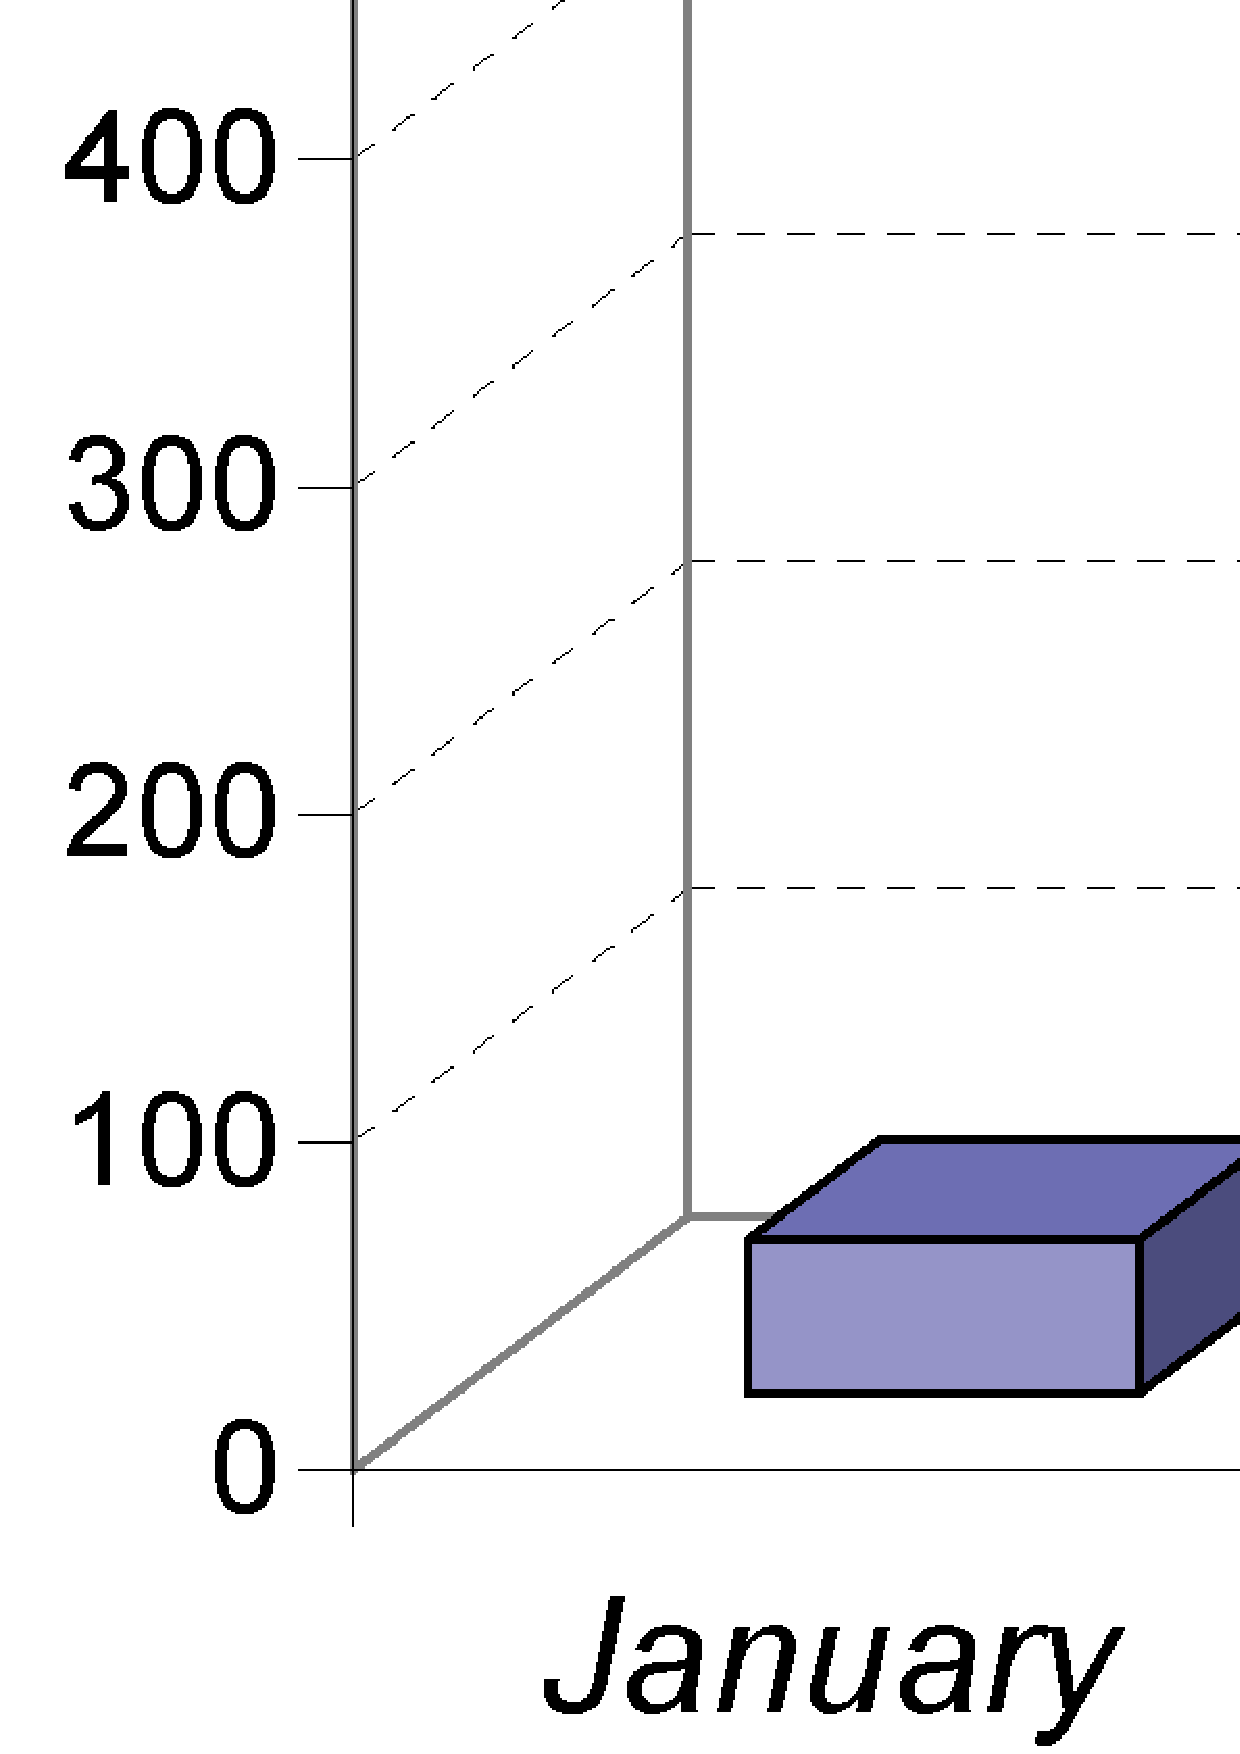
\includegraphics[width=1.00\textwidth]{figures/ClassroomStudyTotalInvocation}
  \caption{Telemetry Analysis Invocation by Month} 
  \label{fig:ClassroomStudyTotalInvocation}
\end{figure}


\begin{figure}[tbp]
  \centering
  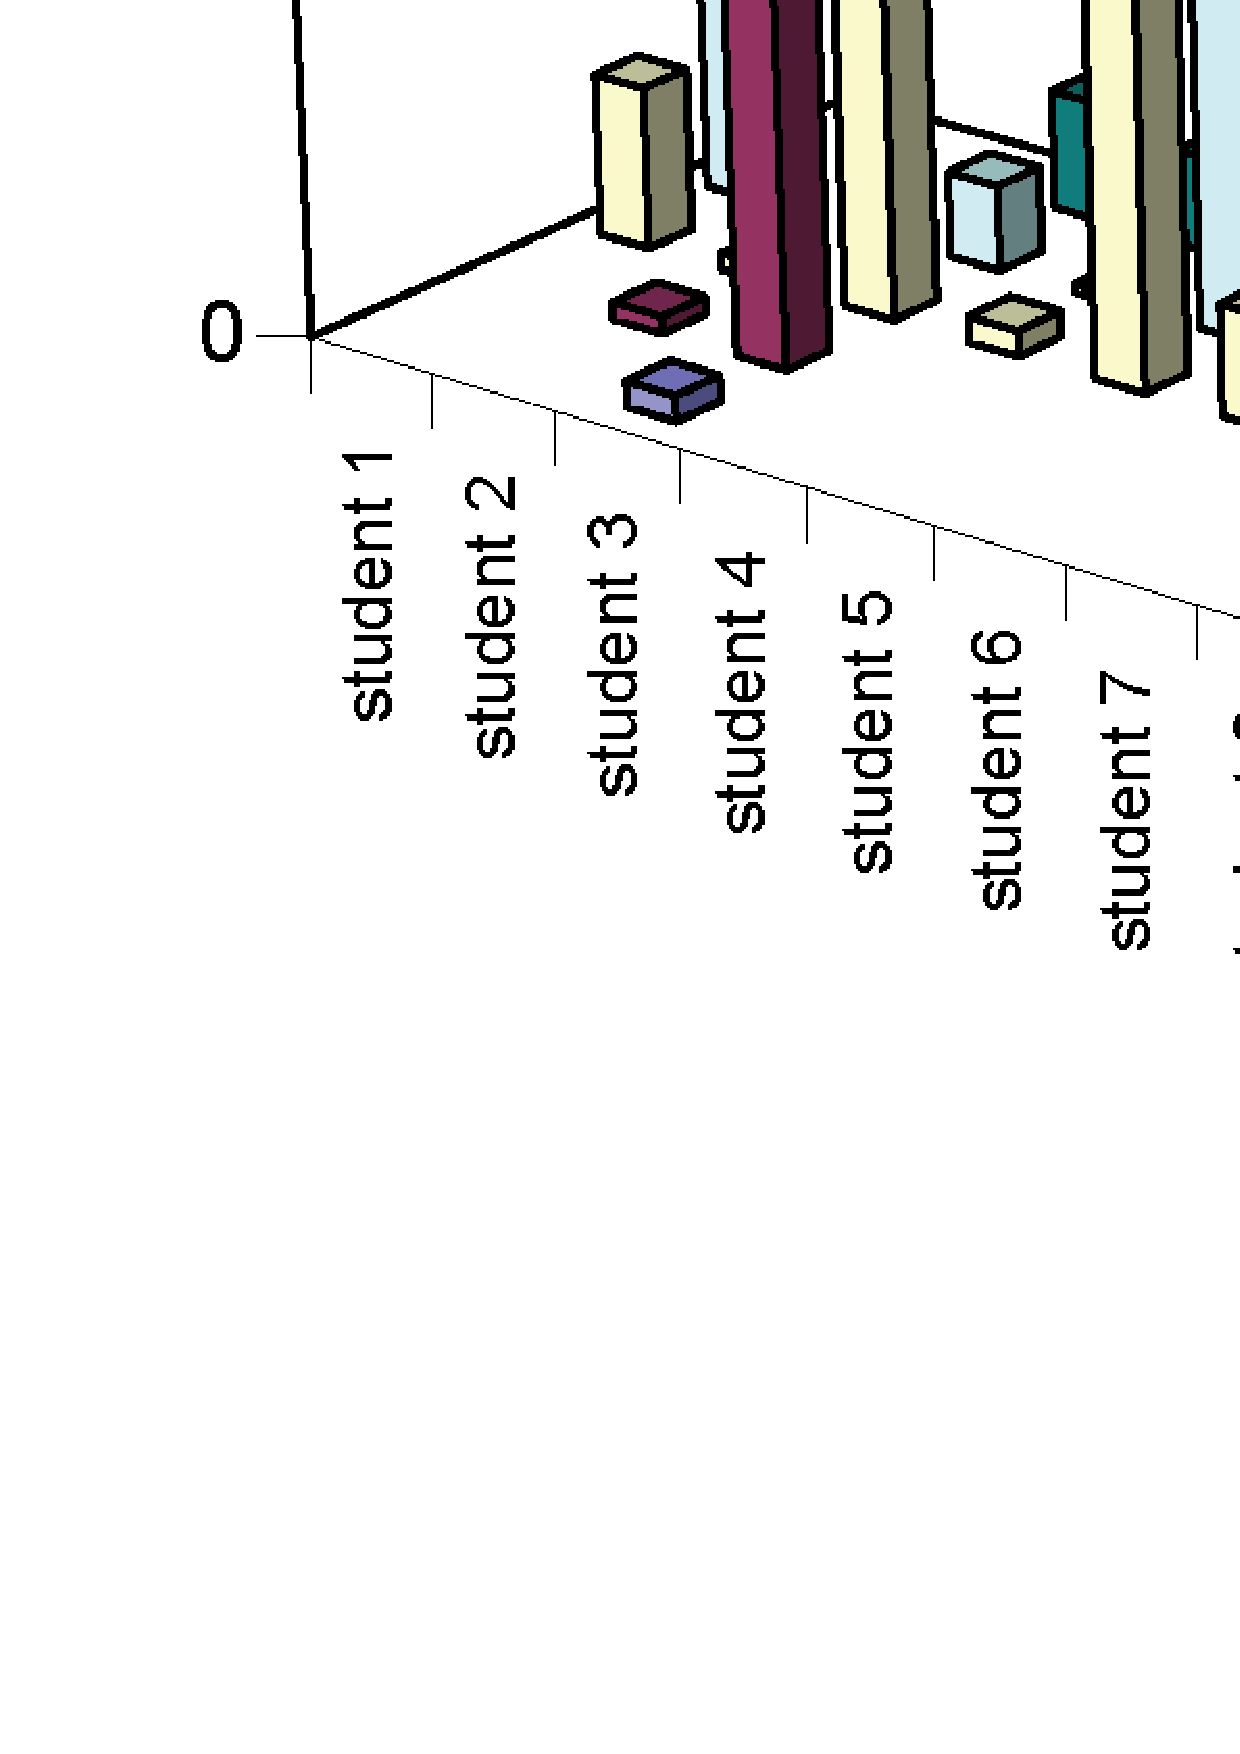
\includegraphics[width=1.00\textwidth]{figures/ClassroomStudyIndividualInvocation}
  \caption{Telemetry Analysis Invocation by Individual and Month} 
  \label{fig:ClassroomStudyIndividualInvocation}
\end{figure}



%%%%%%%%%%%%%%%%%%%%%%%%%%%%%%%%%%%%%%%%%%%%%%%%%%%%%%%%%
%                                                       %
%                   S E C T I O N                       %
%                                                       %
%%%%%%%%%%%%%%%%%%%%%%%%%%%%%%%%%%%%%%%%%%%%%%%%%%%%%%%%%
\clearpage
\section{Study Conclusion}  \label{EvaluationInClassroom:Conclusion}

This study yielded a number of valuable insights into software project telemetry and its implementation.

An automated and unobtrusive metrics collection mechanism is crucial to the success of a metrics program. From the student's feedback, the sensor-based approach appeared to have achieved the goal of eliminating long-term chronic overhead related to metrics collection. However, the one-time setup cost of the sensors was still too high. Though it was not a major issue in the classroom setting, it could cause significant adoption barrier in other environments. Many students had expressed the wish to have an all-in-one intelligent graphical user interface to install and configure the sensors easily. Fortunately, such an installer is now available as a result of user feedback.
	
Software project telemetry appeared to have achieved its design goal of making development process transparent. Most students agreed that they were made more aware of both their own and their team's development process as a result of using the system. However, there was no conclusive evidence to determine whether the increased awareness had actually helped the students improve their software development processes. The data appears to indicate that the ability to understand and interpret telemetry data is related to whether software project telemetry is useful. There were several incidents in which the sensors did not seem to collect metrics correctly, or the telemetry analyses did not seem to compute the data as expected. Some of these were caused by inappropriate interpretation of the results. It seemed that effort-related metrics were most susceptible to mis-interpretation. As far as the implementation was concerned, many students suggested that the web interface for telemetry analysis worked but could be made more user-friendly. 		
	
There was a data privacy issue. Some students seemed to suggest that software project made their development process more transparent than they had wished. They concerned that their personal process data might be misused. I was very well aware of the issue when implementing the system, and had taken steps to limit the kinds of data that could be accessed by people other than the person owning the data. However, it seemed hard to reconcile the conflicting requirements between project management and privacy protection. Some students expressed that they would not want to share personal metrics with others, while other students said they would like to know what other people were doing.

%As with all successful metrics programs, correct interpretation and proper use of metric data are crucial, as well as developer understanding, trust, and support.
	

  \chapter{CSDL Study} \label{Chapter:EvaluationInCSDL}


The previous chapter reported on a classroom study of software project telemetry. The classroom study has the advantage of obtaining insights from a relatively large number of people in a relatively short period of time.  However, it has a number of limitations: the size and the scope of the class projects were relatively small, the time the students could devote to software development activities was relatively limited, and the students in classroom tend to have less software engineering experience.
To mitigate the limitations, I performed another study in the Collaborative Software Development Lab (CSDL) during Spring 2006. The CSDL study had a number of complementary characteristics to the classroom study. Though it involved only five developers and one project manager, the system under development was much larger in scale with almost 300,000 lines of code in total. It had been under development for five years. The CSDL developers had significantly more software engineering experience compared to the developers in the classroom on average. 
Instead of a one-shot survey, I pursued a much more in-depth data collection and analysis strategy over a much longer period of time. 
While still within an academic setting, it intends to provide data that reflect an environment much closer to those in industrial settings.

%In the CSDL study, I introduced software project telemetry as a metrics-based software process improvement program. 

%But before going into details, I want to first make a clarification about the relationship between \textit{Hackystat} and \textit{Software Project Telemetry}. The software under development in CSDL was Hackystat. Software project telemetry was implemented as a Hackystat extension. However, the scope of Hackystat project is much wider than software project telemetry. For example, the Hackystat Project includes other research projects involving high performance computing and test-drive design that are independent from this research on Software Project Telemetry. More detailed information will be provided in the first section of this chapter. You can also refer to Chapter \ref{Chapter:Implementation} for additional information.

This chapter begins with a description of the CSDL setting in Section \ref{EvaluationInCSDL:Setting}.
Section \ref{EvaluationInCSDL:Role} describes my role in the study.
Section \ref{EvaluationInCSDL:StudyDesign} elaborates on the study design.
Section \ref{EvaluationInCSDL:DataCollectionAnalysis} describes data collection and analysis procedures.
Section \ref{EvaluationInCSDL:EventsDescription} reports the results. 
Section \ref{EvaluationInCSDL:StudyConclusion} concludes the chapter with a summary of the insights learned from the study.


%%%%%%%%%%%%%%%%%%%%%%%%%%%%%%%%%%%%%%%%%%%%%%%%%%%%%%%%%
%                                                       %
%                   S E C T I O N                       %
%                                                       %
%%%%%%%%%%%%%%%%%%%%%%%%%%%%%%%%%%%%%%%%%%%%%%%%%%%%%%%%%

\section{CSDL Setting}  \label{EvaluationInCSDL:Setting}

The Collaborative Software Development Laboratory (CSDL) is a software engineering development and research lab at the University of Hawaii. Its mission statement, as published on its website, is ``to provide a physical, organizational, technological, and intellectual environment conductive to collaborative development of software engineering skills.'' 

% Intro of Hackystat
CSDL has been focusing on the development of Hackystat since 2001. Hackystat is a framework for automated metric collection and analysis of empirical software engineering product and process metrics. Several extensions has been developed based on this framework, and are being maintained by the lab. Some of the extensions are specialized to high-level software process analysis, such as Software Project Telemetry as the result of this thesis research, and CGQM for continuous machine-executable Goal-Quality-Metric paradigm. Other extensions are specialized to low-level software process analysis, such as SDSA for micro-process views of software development behaviors at the time scale of minutes or hours, and HPCS for bottleneck identification in the development of parallel programs for high performance computers.
Thus, the scope of the Hackystat project and its framework, includes, but is also much broader than, Software Project Telemetry.


% Intro of Developers
At the time this study was conducted, the Hackystat framework and the extensions maintained by CSDL constituted nearly 300,000 lines of code in total. Figures \ref{fig:HackystatSizeByLanguage} shows the breakdown of size by programming languages. The code was organized into over 70 different modules. 
The development team consisted of one project manager and five on-site developers. The project manager was Dr. Philip Johnson. He was the lab director controlling the overall direction of Hackystat. He also spent a considerable amount of time working on code himself. Three of the developers were Ph.D. students (including me) in software engineering. They were hired by the lab working 20 hours a week. The other two were undergraduate students in their final semester. They were the top students from the undergraduate software engineering class. They were working for the lab in exchange for personal development and course credit.

\begin{figure}[tbp]
  \center
  \includegraphics[width=0.65\textwidth]{figures/HackystatSizeByLanguage}
  \caption{Hackystat Size by Programming Language} 
  \label{fig:HackystatSizeByLanguage}
\end{figure}

% Intro of process and tools.
The team adopted agile software development methods, emphasizing working software as the primary measure of progress. 
The project sources were stored in a \textit{Subversion} repository,\footnote{\textit{Subversion} is a version control system for the management of multiple revisions of the same unit of digital information.} supporting concurrent development by allowing multiple developers to checkout the sources and commit their changes at the same time.
The developers tended to work with a subset of the source code relevant to their assignments. An automated integration build tool was used to handle the full system build and test. Every night, the tool checked out the latest revision of the entire source, compiled, built, and tested the system. If there was any error, an email was sent to the development team. Figure \ref{fig:BuildProcess} is a graphical illustration of the process followed by the developers in the lab.

\begin{figure}[p]
  \centering
  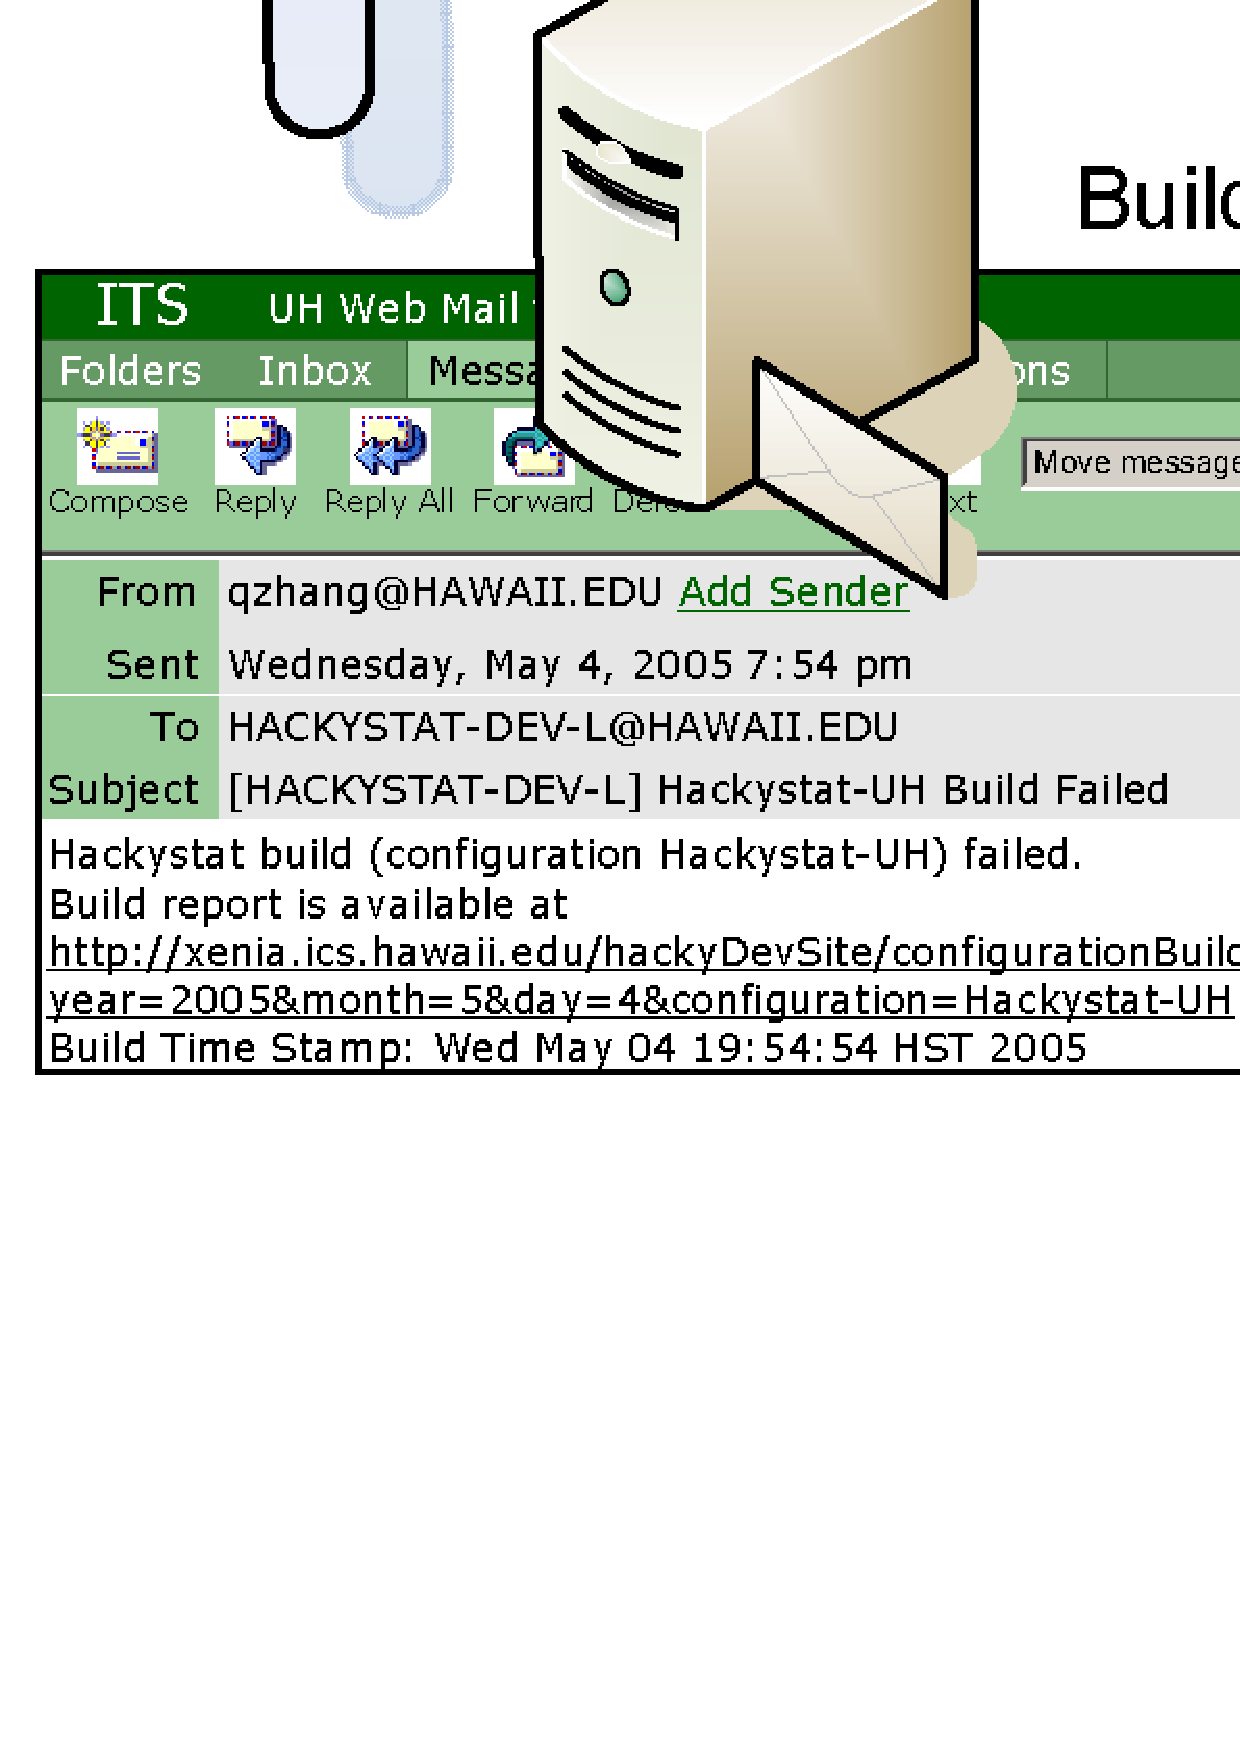
\includegraphics[width=1.00\textwidth]{figures/BuildProcess}
  \caption{CSDL Software Development Process}
  \label{fig:BuildProcess}
\end{figure}

Issues and project progress were tracked by an issue management system called \textit{Jira}. The lab had a status meeting every week. Code review was conducted as needed, but not on a regular basis. Though the team did not treat the software development as a strict \textit{timebox},\footnote{In software project management, a \textit{timebox} is a period of time in which to accomplish some task. The end date is set in stone and may not be changed. If necessary, less functionality than originally planned is provided on the release date.} it made regular releases about every three months.




%\subsection{Communicating Telemetry Analysis Results}

In order to increase the development team's awareness of software metrics, the CSDL development environment was instrumented with sensors to collect a variety of software product and process metrics. These metrics were sent to a server in CSDL for storage and analysis. I wrote a client-side application that automatically extracted telemetry charts from the server on a regular basis and displayed them on a 3x3 array of nine LCD monitors mounted on a wall inside the lab. Figure \ref{fig:TelemetryWall} is a picture of it. I call the nine-monitor wall the \textit{``telemetry wall,''} and the client-side application the \textit{``telemetry control center.''}

\begin{figure}[p]
  \center
  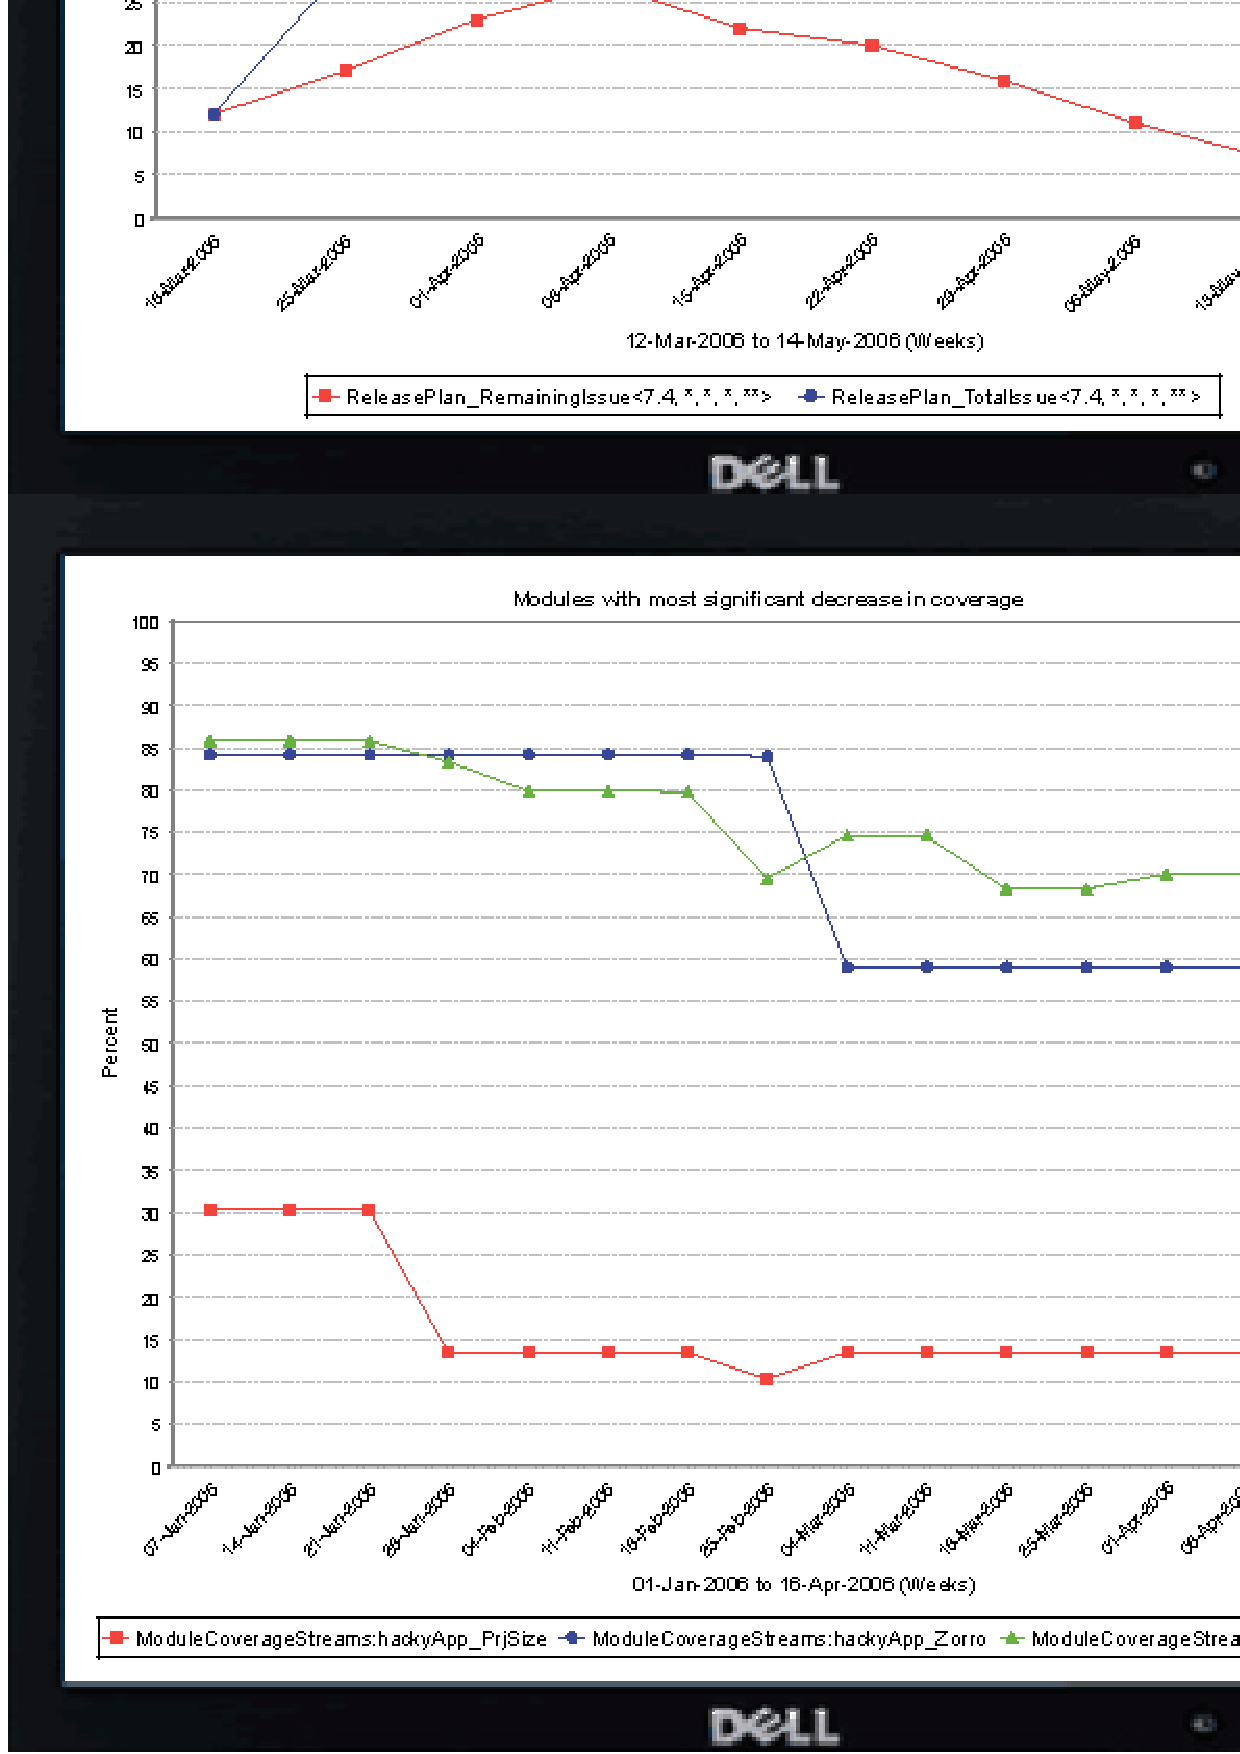
\includegraphics[width=1.00\textwidth]{figures/TelemetryWall}
  \caption{Telemetry Control Center on Telemetry Wall} 
  \label{fig:TelemetryWall}
\end{figure}

A configuration file provided the definitions of the telemetry charts to be displayed
using the standard telemetry language constructs (Section \ref{Telemetry:Component}). The telemetry control center retrieved the charts through the telemetry expert analysis interface (Figure \ref{fig:TelemetryExpertAnalysis}) provided by the software project telemetry implementation (Chapter  \ref{Chapter:Implementation}). The charts on the nine monitors formed a \textit{``telemetry scene.''} The telemetry control center application could be configured to cycle through different scenes automatically. 

The telemetry wall made a sequence of telemetry charts continuously available to the entire team automatically without any action on the part of the developers or the project manager. Rather than having to wait for a status update meeting, they could simply look at the telemetry wall to get a perspective on the current state of development. The development team had access to the regular telemetry analysis interface (Figure \ref{fig:TelemetryExpertAnalysis} and   \ref{fig:TelemetryReportChartStream}) through a web browser as well. However, the primary way I used to communicate telemetry analysis results to the team was the telemetry wall. It made it easy to discuss telemetry charts either formally in CSDL meetings or casually during lunch hours. 









%%%%%%%%%%%%%%%%%%%%%%%%%%%%%%%%%%%%%%%%%%%%%%%%%%%%%%%%%
%                                                       %
%                   S E C T I O N                       %
%                                                       %
%%%%%%%%%%%%%%%%%%%%%%%%%%%%%%%%%%%%%%%%%%%%%%%%%%%%%%%%%
\section{Researcher's Role}  \label{EvaluationInCSDL:Role}

My affiliation with CSDL started in 2003. I implemented the software project telemetry system as an extension to Hackystat. Dr. Philip Johnson is the director of CSDL. He is my dissertation adviser. He is also the project manager of Hackystat. I received a cornucopia of helpful advice from him during my implementation of software project telemetry.

During the period of this study, I acted as an on-site process expert introducing software project telemetry as a metrics-based process improvement program. I took careful observation of the team's development activity. I interviewed the team members and the project manager. I defined telemetry charts and made them available on the telemetry wall (Figure \ref{fig:TelemetryWall}). I discussed telemetry analysis results with the developers and the project manager. I recommended process changes. I helped the project manager institute changes to improve project management practices. I also helped the developers gain insights into their development processes.

At the same time, my own software development effort was concentrated on improving software project telemetry implementation based on the feedback received in this study. It included: (1) making sensors and telemetry charts available to meet the team's process-improvement and decision-making requirements, (2) enhancing the telemetry language to improve the display of telemetry charts, and (3) profiling and eliminating telemetry analysis runtime performance bottlenecks.









%%%%%%%%%%%%%%%%%%%%%%%%%%%%%%%%%%%%%%%%%%%%%%%%%%%%%%%%%
%                                                       %
%                   S E C T I O N                       %
%                                                       %
%%%%%%%%%%%%%%%%%%%%%%%%%%%%%%%%%%%%%%%%%%%%%%%%%%%%%%%%%
\section{Study Design}  \label{EvaluationInCSDL:StudyDesign}

%In the classroom study, I was able to gather insights from a relatively large number of people in a relatively short period of time. But the classroom study had limitations. The CSDL study was designed to have contrasting strengths and limitations. Unlike the classroom environment, there were a relatively small number of study participants in CSDL: five developers and one project manager. However, the project under development was much larger in scale. It contained nearly 300,000 lines of code in total, and had been underdevelopment for five years. The CSDL developers had significantly more software engineering experience and process maturity compared to the average student in the classroom.

The CSDL study was a mix-methods study to explore the use of software project telemetry in depth.
I have been affiliated with the lab for three years. Because of my familiarity with the CSDL software development environment and the small number of developers involved in the study, I was able to pursue a much more comprehensive data collection and analysis strategy over a much longer period of time compared to the classroom study. Instead of just giving the developers software project telemetry tools and observing how they used them, I took a more active role by acting as a process expert. I introduced software project telemetry as a metrics-based process improvement program. I proposed improvements to the CSDL software development process, and helped the project manager institute the changes. The steps I took consisted of the following iterative steps: %(Figure\ref{fig:CsdlStudyMethod}):

\begin{enumerate}
  \setlength{\itemsep}{0pt}
  \setlength{\parskip}{0pt}
	\item Collect data from observations and interviews.
	\item Code the data in order to generate hypotheses.
  \item Propose improvements to the CSDL software development process.
  \item Continue to collect data to assess the effectiveness of the changes.
  \item Draw conclusions from the data gathered.
\end{enumerate}
  
%\begin{figure}[p]
%  \center
%  \includegraphics[height=0.80\textheight]{figures/CsdlStudyMethod}
%  \caption{CSDL Research Strategy} 
%  \label{fig:CsdlStudyMethod}
%\end{figure}

The study involved many elements from the constructivist paradigm. It was a case study in which I explored the use of software project telemetry in CSDL extensively. I collected data from observations and interviews, and generated hypotheses from the data. My observation strategy was complete involvement as a full participant instead of an outside spectator. I was in the lab almost every day working with the developers, and attended every weekly status update meeting. My interview strategy was in-depth interview instead of structured interview. Both formal and informal interviews were used. I always encouraged free responses. The purpose was to gather much richer data about how the developers and the project manager interacted with software project telemetry to make decisions. I have to admit that my affiliation with CSDL was a source of bias. Years of affiliation might have ingrained in me the software process practiced in CSDL, and thus made me unable to see important information in my observations and interviews. However, the bias was mitigated through several factors. My observation was much less disruptive to the developers than having a stranger watching over their backs. My detailed knowledge about the project under development made it easy for me to link the observed facts to the contextual information in CSDL, so that I could have much deeper insights into ``what's going on'' than an outsider. I often reconciled my interpretation of observed facts with the developers and the project manager in interviews.

The study also involved an element from the post-positivist paradigm. After the hypotheses were generated, I tested them in a limited way by making changes to the telemetry system or implementing new facilities to see if the hypothesized outcome would come true. 
To some extent, this hypothesis testing procedure could be viewed as the simplest and uncontrolled form of experiment. The difference is that most experiments rely on statistical analysis to draw conclusions, but mine does not.


 






%%%%%%%%%%%%%%%%%%%%%%%%%%%%%%%%%%%%%%%%%%%%%%%%%%%%%%%%%
%                                                       %
%                   S E C T I O N                       %
%                                                       %
%%%%%%%%%%%%%%%%%%%%%%%%%%%%%%%%%%%%%%%%%%%%%%%%%%%%%%%%%
\section{Data Collection and Analysis} \label{EvaluationInCSDL:DataCollectionAnalysis}

My data came from both observations and interviews. The observations included almost everything related to CSDL software development. The interviews covered a variety of topics, from the discussion of the current development process and telemetry analysis results, to the exploration of improvement options and assessment of change impact.

The data were stored and organized using a software program called \textit{``Confluence.''} The reason that I used the software was because of the ease with which different types of documents could be organized and accessed anywhere through a web interface. Though Confluence is mainly designed for knowledge sharing, I did not share my field notes with the study participants. I divided the \textit{Confluence} data storage area into two sections: ``Raw Data'' and ``Hypotheses.'' At the end of the study, I had accumulated a total of 173 entries in the ``Raw Data'' section, and generated a total of 9 findings in the ``Hypotheses'' section.

\begin{itemize}
	\item \textbf{Raw Data} --- They were field notes from observations and informal interviews, and transcripts from formal interviews. The data in this category were further organized into two levels. Second level entries were immediate follow-up observations and interviews closely related to their parent entry in the first level. The total 173 entries in this section consisted of 109 first level entries and 64 second level entries. Figure \ref{fig:CSDL-RawData1} shows an index page with links to all raw data entries, while Figure \ref{fig:CSDL-RawData2} shows the details of one of the entries. The raw data themselves cannot be published because of privacy issues. However, I included a summary for each first level entry in Appendix \ref{Appendix:DataInCSDL}. The summaries were assigned unique identification numbers, which were referenced in my discussion of the study results in Section \ref{EvaluationInCSDL:EventsDescription}. The intention is to provide the reader a mechanism to ``audit'' my conclusions in some sense.

  \item \textbf{Hypotheses} --- They were hypotheses regarding the use of software project telemetry from my conceptualized ideas based on the raw data. All entries in this section were formatted into five subsections: (1) pre-hypothesis links to raw data entries, (2) generated hypothesis, (3) change implementation, (4) post-hypothesis links to raw data entries, and (5) conclusion. Figure \ref{fig:CSDL-Hypothesis1} is an index page with links to all generated hypotheses, while Figure \ref{fig:CSDL-Hypothesis2} shows the details of one of the hypotheses. The details of each finding were reported in Section \ref{EvaluationInCSDL:EventsDescription}.

\end{itemize}


The approach I followed to generate hypotheses from the data was inspired by grounded theory. 
As soon as the field notes and interview transcripts were entered into the raw data section, I applied \textit{``open coding''} to label the text with different category names (i.e., \textit{``conceptualization''} of ``what's going on'' in grounded theory terminology). The coding was done as annotations to the raw data text (Figure   \ref{fig:CSDL-RawData2}), and was stored together with the raw data entry. I constantly compared, modified, and merged the category names when new data came in. During the process of \textit{open coding}, some themes (i.e., \textit{``core variables''}) emerged naturally. They were related to the use of software project telemetry. I continued to collect and categorize data after the emergence of the themes. However, at this step, my data collection was more selective. I paid more attention to those related to the identified themes (i.e., \textit{``selective coding''}).
The next step was \textit{``theoretical memoing''}, in which I generated my hypotheses, such as the best practice of software project telemetry, the plausible reason for the problems encountered during its use, and the possible remedy to improve the system. The hypotheses were entered in the ``hypotheses'' section in the Confluence data store, together with the links to the relevant raw data entries. I did not have a separate \textit{``sorting''} step. The links to the relevant raw data in each hypothesis entry served the same purpose as sorting.
In contrast to grounded theory where hypotheses are the end goal, my data collection and analysis did not stop there. After the hypotheses were generated, I made changes to the telemetry system, implemented new facilities, and collected additional data in an attempt to confirm or refine the hypotheses. The additional data were recorded in the ``raw data'' section as well, and any refinement to the previously generated hypotheses was also noted in the ``hypotheses'' section.


\begin{figure}[p]
  \center
  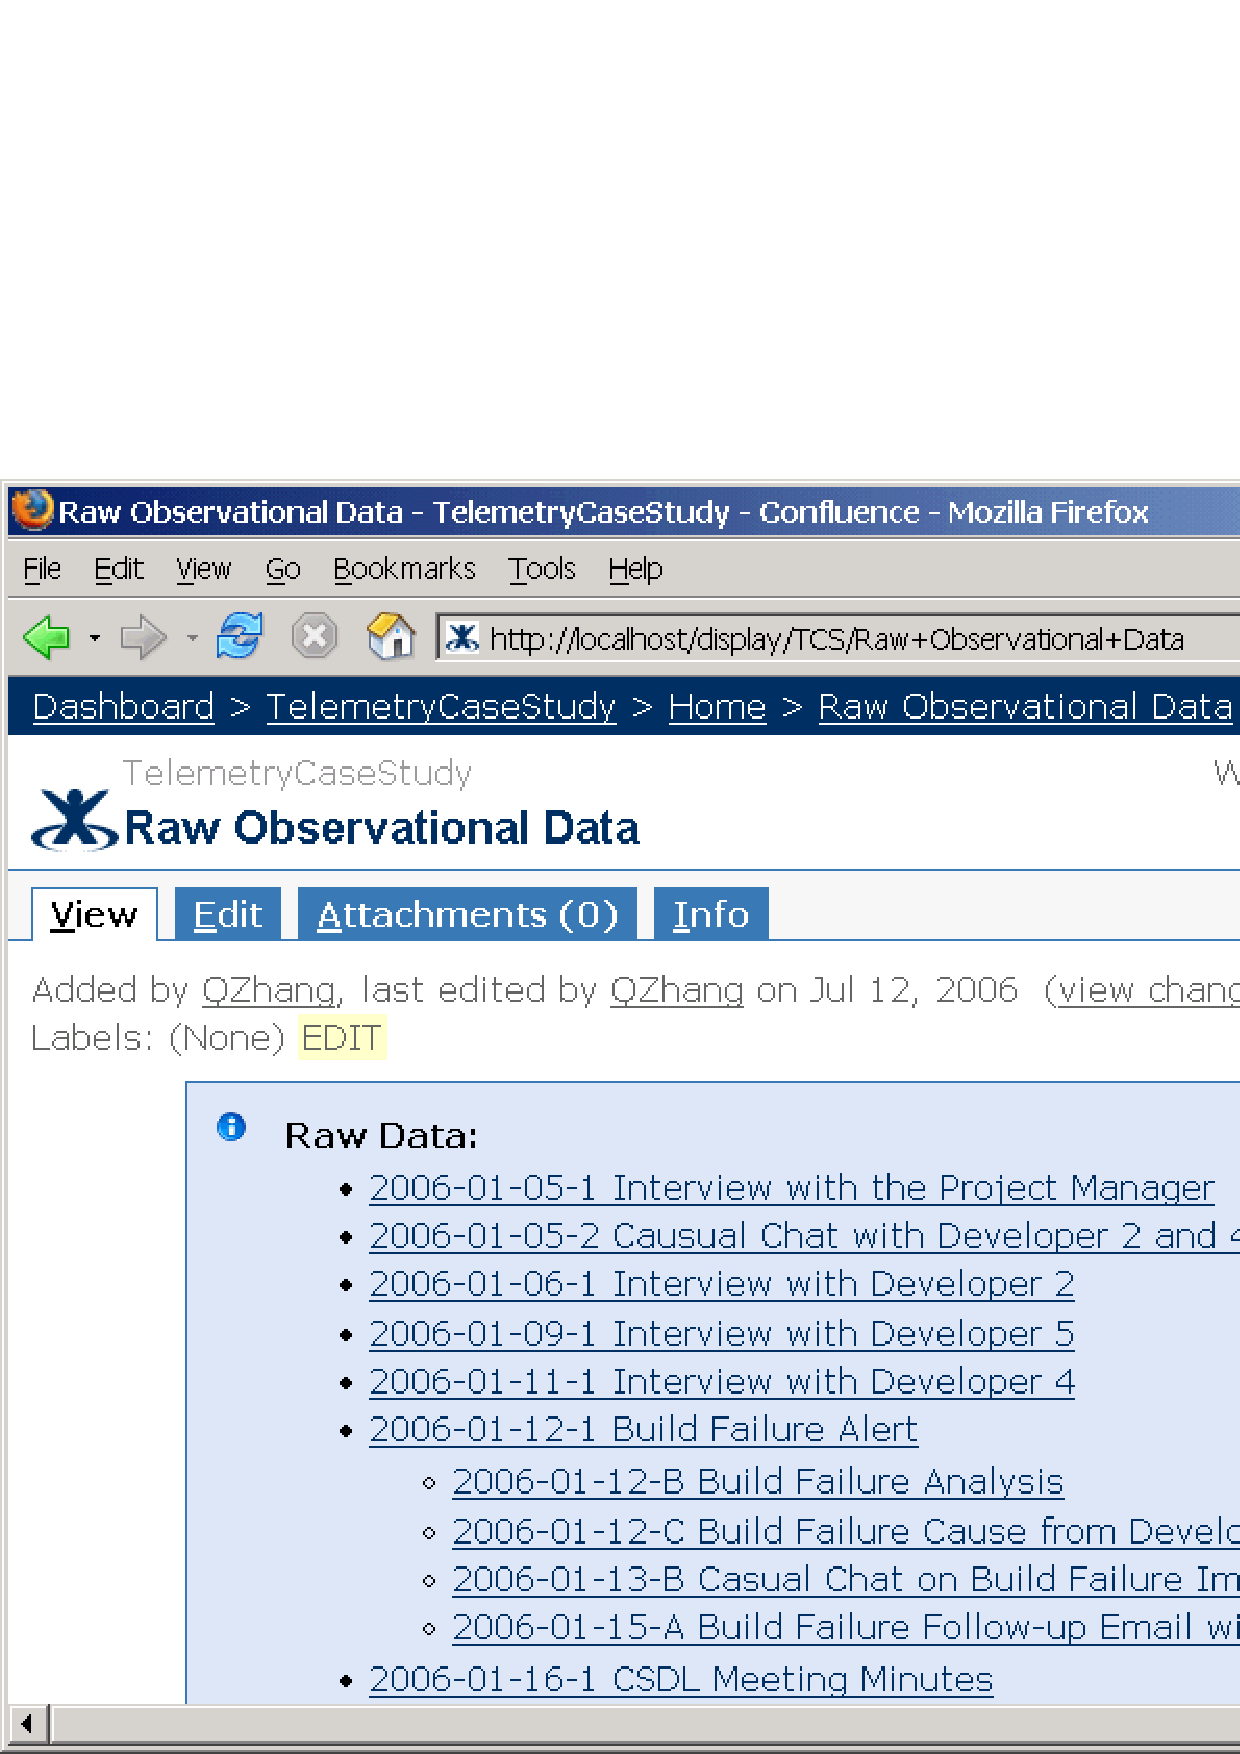
\includegraphics[width=1.00\textwidth]{figures/CSDL-RawData1}
  \caption{A Page with Links to all Raw Data Entries} 
  \label{fig:CSDL-RawData1}
\end{figure}
	
\begin{figure}[p]
  \center
  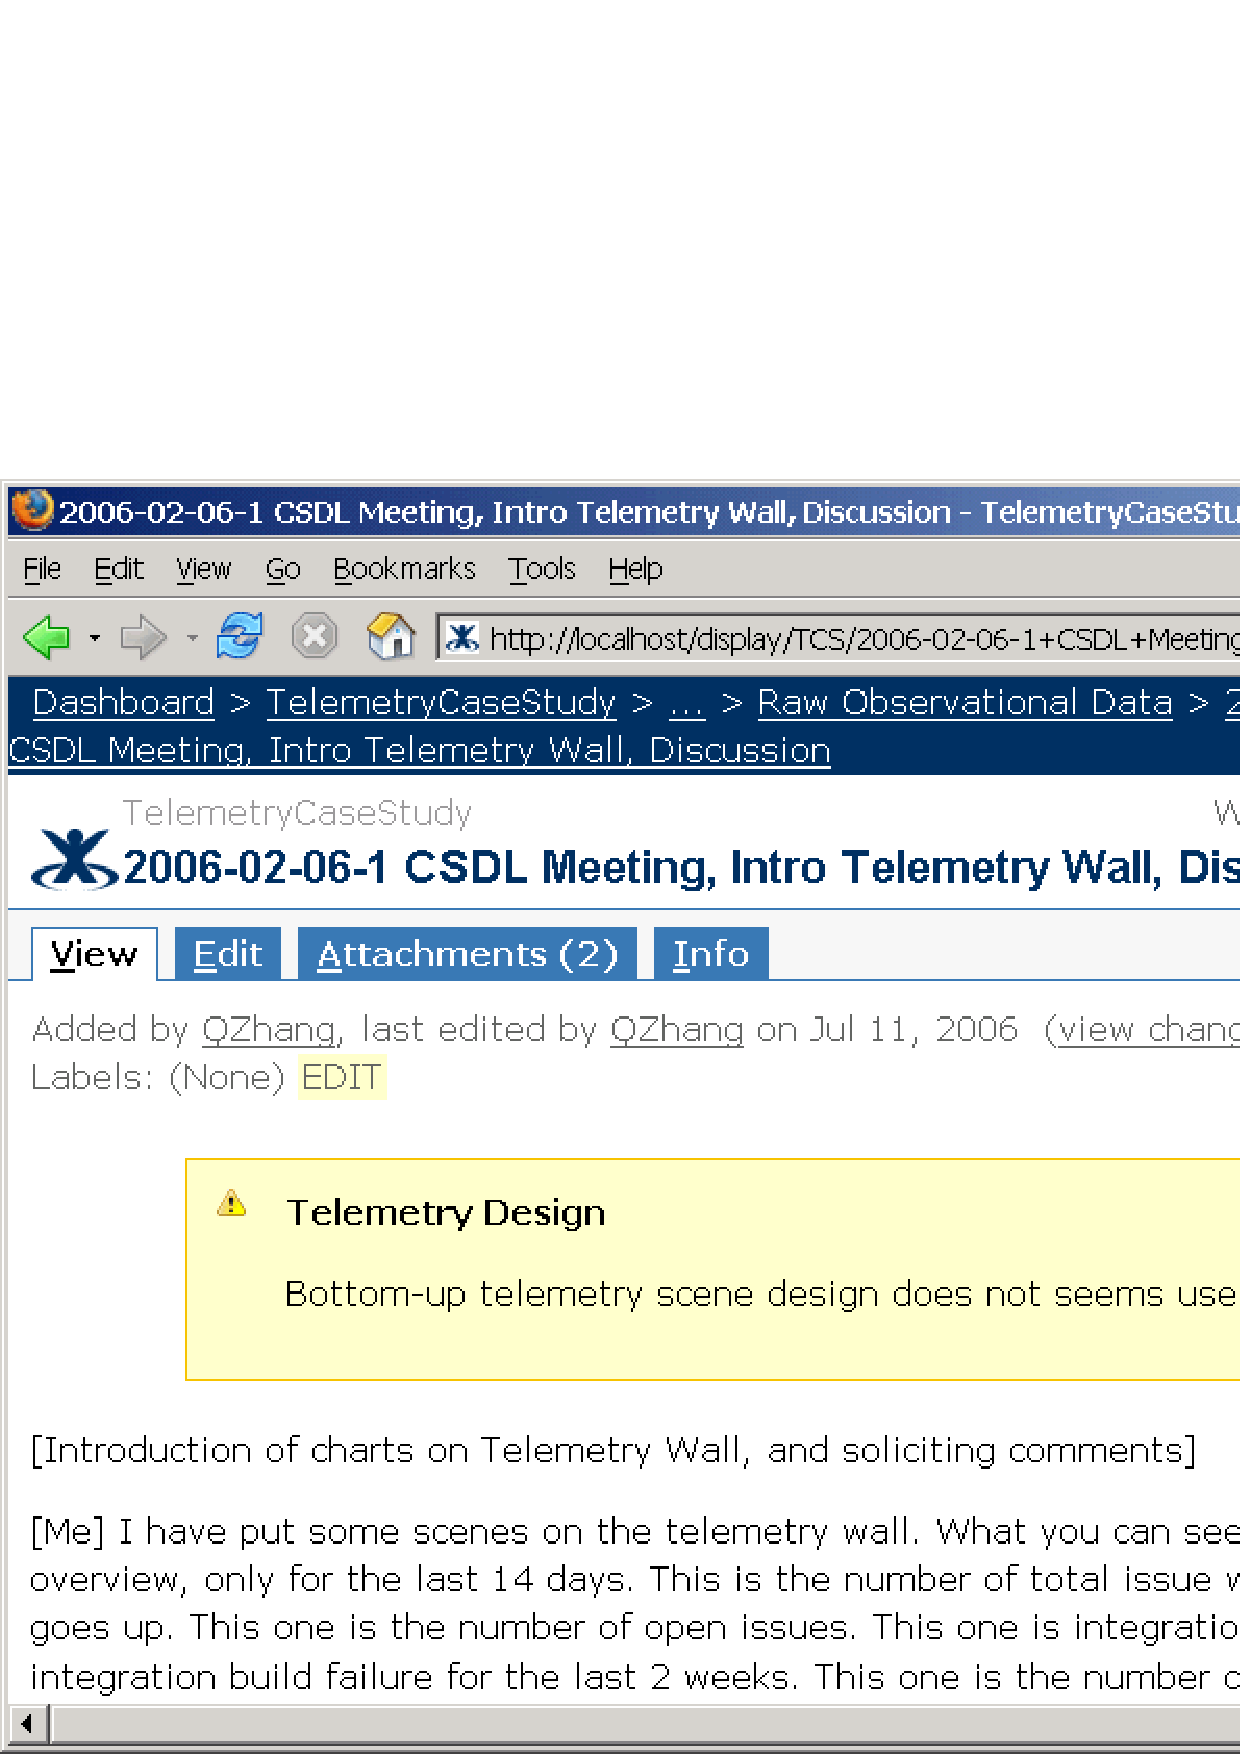
\includegraphics[width=1.00\textwidth]{figures/CSDL-RawData2}
  \caption{One of the Raw Data Entries with Annotation} 
  \label{fig:CSDL-RawData2}
\end{figure}	
	

\begin{figure}[p]
  \center
  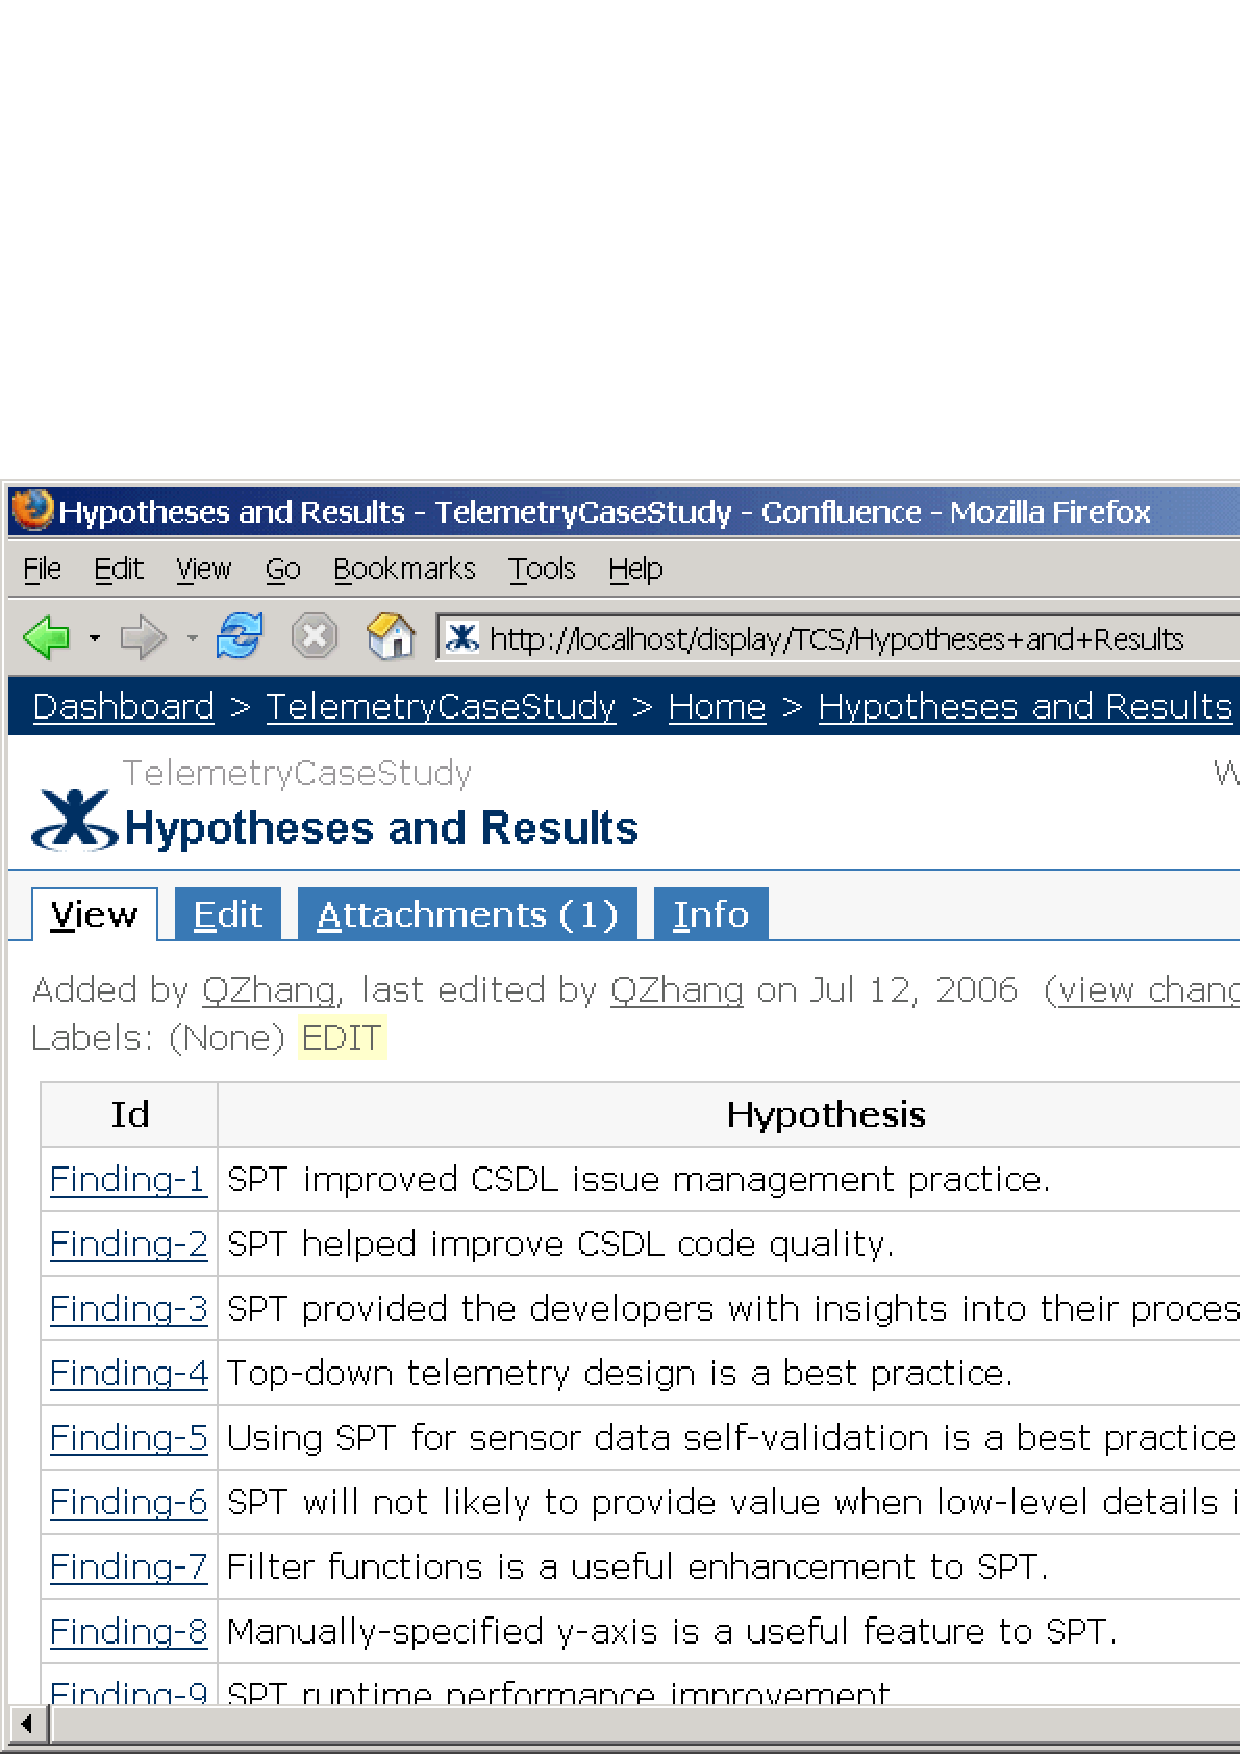
\includegraphics[width=1.00\textwidth]{figures/CSDL-Hypothesis1}
  \caption{A Tables with Links to all Generated Hypotheses} 
  \label{fig:CSDL-Hypothesis1}
\end{figure}

\begin{figure}[p]
  \center
  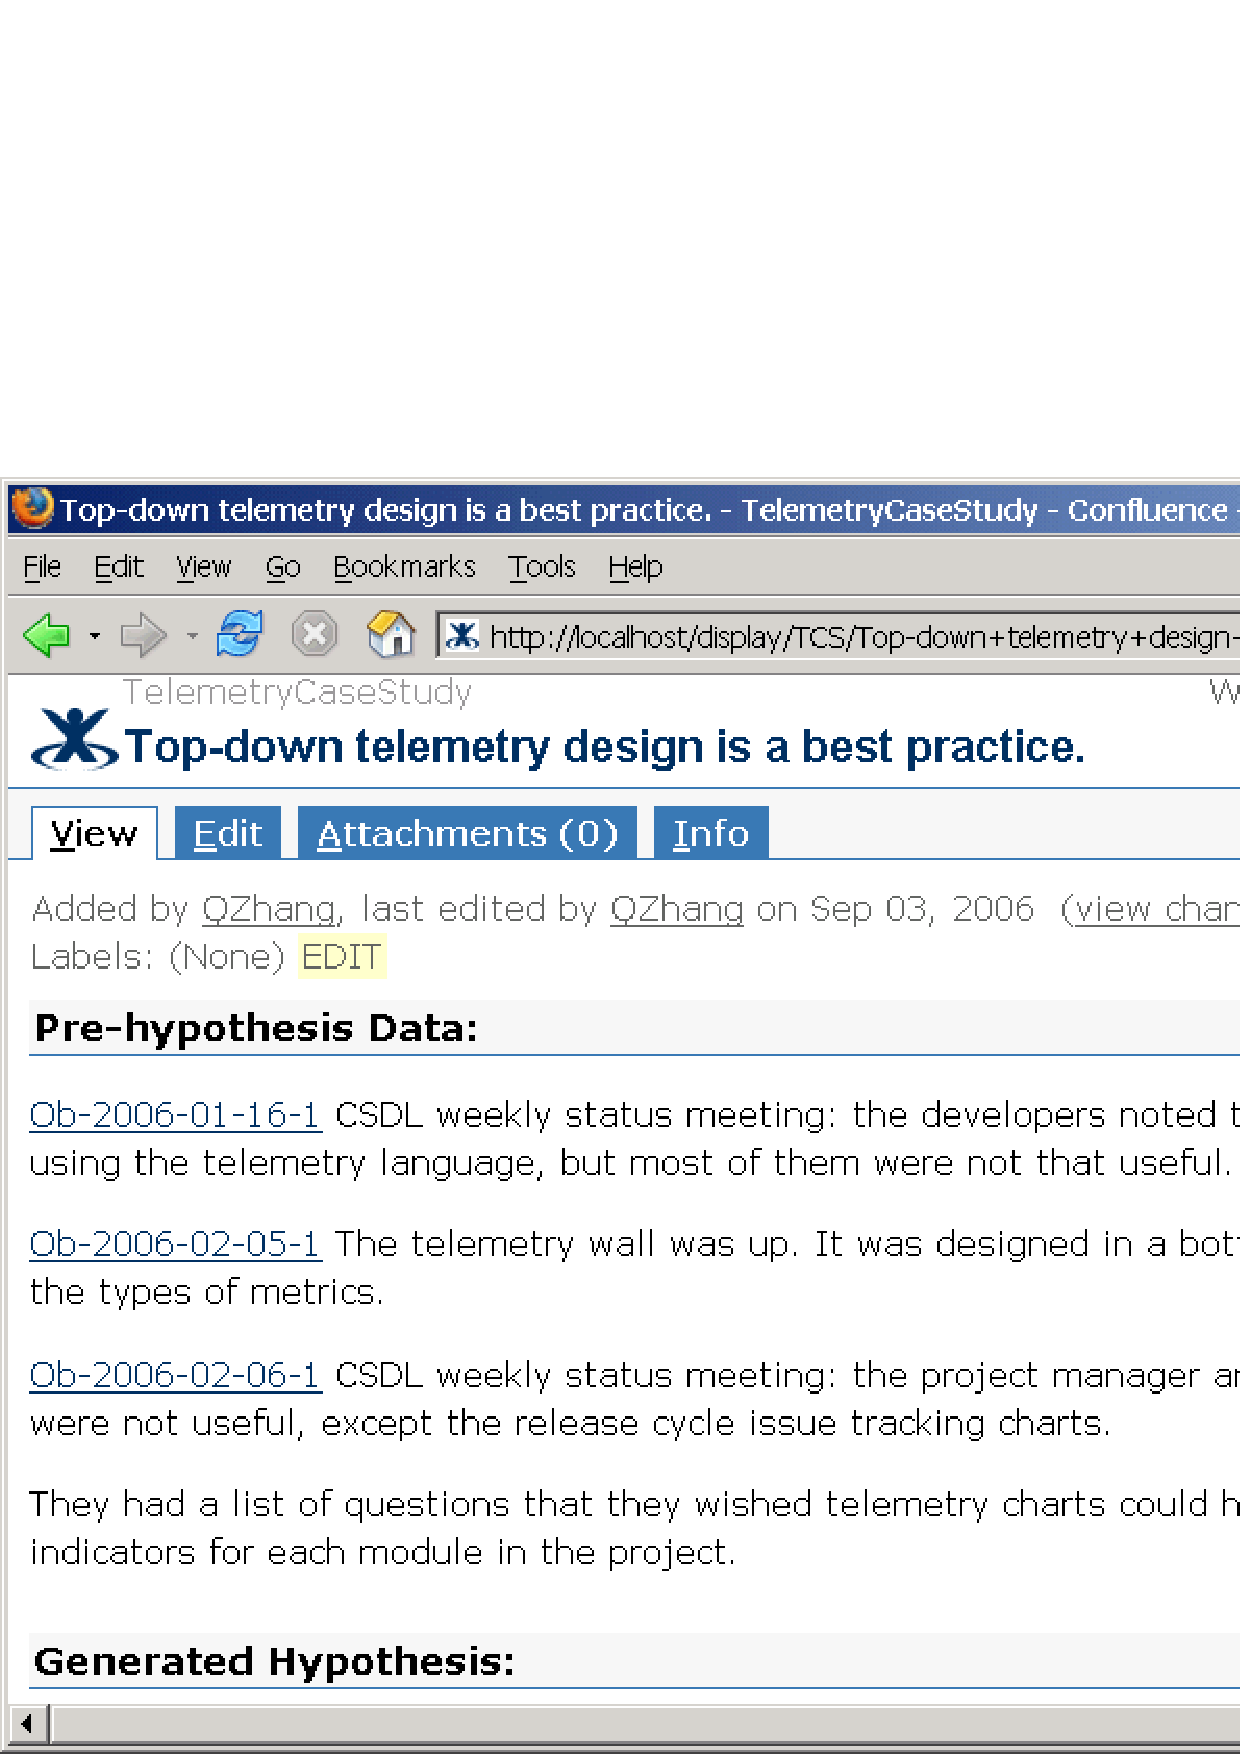
\includegraphics[width=1.00\textwidth]{figures/CSDL-Hypothesis2}
  \caption{One of the Generated Hypotheses} 
  \label{fig:CSDL-Hypothesis2}
\end{figure}








%%%%%%%% Sub Section %%%%%%%%%
%\clearpage
%\subsection{Quantitative Data}
%
%\textcolor{red}{To be removed}
%
%Quantitative data were collected from software product and process metrics.
%The CSDL development environment was heavily instrumented. In order to collect software process metrics, sensors were attached to the IDEs on the developers' workstations, to the SVN source code repository, to the Jira issue management system, and to the nightly integration build system. In order to collect software product metrics, a set of code analyzers were invoked automatically on software artifacts every night. 
%
%Sensors were everywhere. The metrics collection practice in CSDL was to collect whatever metrics possible regardless of whether you could think of a use for such metrics or not. The rationale behind the practice was the low cost associated with the sensor-based metrics collection mechanism. In addition, by using as many sensors as possible, the lab was able to assess and improve the quality of the sensors and also determine how the server behaved under load. All the sensors send metrics to a server located inside CSDL. The metrics were used as input for telemetry analysis.
%
%\begin{figure}[p]
%  \center
%  \includegraphics[width=1.00\textwidth]{figures/CSDL-QuantitativeData1}
%  \caption{\textcolor{red}{TO BE UPDATED:} CSDL Study Quantitative Data Overview} 
%  \label{fig:CSDL-QuantitativeData1}
%\end{figure}
%
%\begin{figure}[p]
%  \center
%  \includegraphics[width=1.00\textwidth]{figures/CSDL-QuantitativeData2}
%  \caption{\textcolor{red}{TO BE UPDATED:} CSDL Study Quantitative Data Drilldown} 
%  \label{fig:CSDL-QuantitativeData2}
%\end{figure}







%%%%%%%%%%%%%%%%%%%%%%%%%%%%%%%%%%%%%%%%%%%%%%%%%%%%%%%%%
%                                                       %
%                   S E C T I O N                       %
%                                                       %
%%%%%%%%%%%%%%%%%%%%%%%%%%%%%%%%%%%%%%%%%%%%%%%%%%%%%%%%%

\section{Results} \label{EvaluationInCSDL:EventsDescription}

The results of the study are the findings regarding the use of software project telemetry. Each finding is reported in its own sub-section, which is organized into the following parts:

\begin{itemize}
	\item \textbf{Pre-hypothesis Data}\footnote{To preserve privacy, I used the word \textit{``he''} when referring to individual developer throughout my report, even though there were both male and female participants in the study.} --- Summary information about the data I collected that led to the generated hypothesis.

	\item \textbf{Generated Hypothesis} --- The hypothesis, such as the best practice of software project telemetry, the plausible reasons for the problems encountered during its use, and the possible remedies to improve the system.
	
	\item \textbf{Intervention} --- The changes I introduced based on the hypothesis in order to use software project telemetry more effectively, or overcome the problems encountered during its use.
	
	\item \textbf{Post-hypothesis Data}\footnote{Same as above.} --- The additional data I collected after the changes were implemented, which were used to confirm or refine the generated hypothesis. 
	
	\item \textbf{Conclusion} --- The final finding and comments.
	
\end{itemize}
	
Finally, at the end of each report, I included an ``elaboration'' to provide much more detailed account of the finding.

%This section reports on several experiences from applying \textit{software project telemetry} in CSDL as a metrics-based process improvement program. Some experiences were successful. Some were not. Both types are reported in this section, and conclusions were drawn in the next section (Section \ref{EvaluationInCSDL:StudyConclusion}).






%%%%%%%%%%%%%%%
%  S T O R Y  %
%%%%%%%%%%%%%%%
\clearpage
%\subsection{Software project telemetry improved CSDL issue management practice.}
\subsection{Improvement on CSDL Release Cycle Issue Management}
\label{EvaluationInCSDL:EventsDescription:ProjectIssueTracking}

\subsubsection{Pre-hypothesis Data:}
\begin{itemize}
  \setlength{\itemsep}{0pt}
  \setlength{\parskip}{0pt}
  \item 2006-01-05-1: I discussed the existing analysis of issue metrics with the project manager in an interview. He did not utilize the metrics in project management, because the analysis was inadequate for release cycle planning and tracking. 
	\item 2006-01-05-2: I interviewed two developers on their opinions about the utility of the metrics currently collected in the lab. One of them thought the issue related metrics were not that useful, because they were quite different from what he had anticipated. 
	\item 2006-01-06-1: I discussed the current status of issue management with a developer, who told me that most of his development activities were not recorded in the issue database.
	\item 2006-01-09-1: I held a discussion with another developer, who estimated that only 20\% - 30\% of his development activities were tracked by the issue database. He also told me that he never followed the issue priority in resolving issues assigned to him.
	\item 2006-01-11-1: I held a discussion with yet another developer, who estimated that less than 15\% of his development activities were tracked by the issue database. He told me that most of his issues were assigned through emails instead of the issue management system. He also told me that he did not understand how issue metrics were computed.
\end{itemize}
	
\subsubsection{Generated Hypothesis:}
There were two reasons why the issue metrics were not useful: (1) the issue tracking system severely under-represented the actual development effort; and (2) the issues scheduled for a release did not reflect the actual items that the team wanted to accomplish in that release cycle. If these two problems could be resolved, then the issue tracking telemetry charts could be used not only to track the progress in a release cycle, but also to make in-process predictions about the release schedule. 

\subsubsection{Intervention:}
I identified the problem to the project manager and the developers, and explored options with them to make the issue tracking database more consistent with the actual development effort.

\subsubsection{Post-hypothesis Data:}
\begin{itemize}
  \setlength{\itemsep}{0pt}
  \setlength{\parskip}{0pt}
	\item 2006-01-16-1: The project manager discussed possible changes to improve the issue management practice with the developers in a weekly status meeting.
	\item 2006-01-19-2: As part of corrective measures, the project manager went through all issues and tagged them with realistic fix version numbers to get ready for the new release cycle (i.e., Release 7.3).
	\item 2006-01-19-3: As part of corrective measures, the project manager sent out an email requiring that all future commits should have issue Id in commit log comment field.
	\item 2006-01-23-2: This was the first time in my observation that the new issues assigned in the weekly status meeting were recorded in the issue management system.
	\item 2006-01-29-1: I enhanced the Jira sensor to collect missing information required for issue tracking telemetry analyses.
	\item 2006-02-03-1: I made the issue tracking charts available on the telemetry wall, and showed them to a developer. He commented that they could be used not only to track issue status but also to predict system release date.
	\item 2006-02-06-1: The project issue tracking charts were formally introduced in a CSDL meeting. The project manager commented that they were ``highly useful.''
  \item 2006-03-13-1: I interviewed a developer. He confirmed that almost all his work was tracked by the issue tracking system now.  
  \item 2006-03-15-2: I interviewed two more developers. They all confirmed that most of their work was tracked by the issue tracking system.
	\item 2006-03-20-2: The project manager reviewed the issue tracking chart after release 7.3 was finished, and reflected that the chart helped him determine whether more issues could be added to that release. 
  \item 2006-04-07-3: The project manager was comparing release 7.4 issue tracking chart with the chart from the previous release cycle to make short term predictions.
  \item 2006-04-26-1: During an interview, the project manager told me that his project management skill had improved a lot with respect to release cycle issue tracking and planning.
\end{itemize}

\subsubsection{Conclusion:}
The additional data appears to confirm the hypothesis. The corrective measures were simple but effective. The issue tracking charts were found useful by the project manager for release cycle progress tracking and in-process prediction.

\subsubsection{Elaboration:}

CSDL used an issue management tool called \textit{``Jira''} to record and track issues related to the \textit{Hackystat} development. The types of the issues managed by \textit{Jira} included feature requests, task assignments, and software bugs. CSDL had been using \textit{Jira} and collecting issue related metrics for almost two years.
During an interview at the beginning of this study, the project manager revealed that he did not utilize the issue metrics to plan and track issues in a release cycle. I also interviewed the developers asking them their opinions about the metrics being collected in CSDL. One of them identified the issue metrics as one of not-so-useful metrics. Two problems were identified in the discussions, both related to the way issues were managed and tracked:

\begin{itemize}
  \item The issue management system significantly under-represented the actual development effort. For example, the percentage of issues tracked by \textit{Jira} was less than 15\% according to one developer. Another developer estimated this number between 20\% to 30\%. A lot of issues were assigned in emails or weekly status meetings, instead of through the issue management system.
  
	\item The open issues in the issue management system did not correspond to the expectation for the set of items to be accomplished in a release cycle. I raised this problem in an interview with the project manager. In his own words, when preparing for a stable release, he simply \textit{``chucked the remaining unresolved issues over the fence into the next version.''}
\end{itemize}

My hypothesis was that the issue metrics were not useful precisely because of the two problems identified above. If the issue tracking database could be made consistent with the actual development effort, then the issue telemetry charts could be used not only to track the progress in a release cycle, but also to make in-process predictions about the release schedule.

After I identified the problems to the project manager and the developers, they took corrective measures quickly. On the manager side, the project manager went over all the issues, prioritized them, and tagged them with realistic fix version numbers. On the developer side,	the developers were required to supply a log message referencing an issue number whenever making a commit. The idea was that the practice would remind them to create a \textit{Jira} issue if it had not already existed.

The result of these changes was both effective and positive, because they made it possible to generate issue tracking charts that reflected the actual development activities. For example, Figure \ref{fig:CSDL-Issue730} and \ref{fig:CSDL-IssueActiveTime730} were taken from the Hackystat release cycle 7.3, which lasted from mid-January to mid-March.

Figure \ref{fig:CSDL-Issue730} is a telemetry chart showing the number of total \textit{vs.} remaining issues on the last day of each week during the Hackystat 7.3 release cycle. The blue line on the top is the total number of issues scheduled for that release, while the red line below is the number of remaining issues. The telemetry chart clearly indicates that CSDL did not schedule everything up-front but rather added new issues almost every week. There was a concern that adding new issues constantly might lead to unmanageable release cycles. However, the project manager told me that he used the trend about issue closure in the red line to control whether or not more issues could be added to the release cycle. As the chart indicates, after initial weeks of issue build-up, CSDL was able to make consistent progress toward zero open issue and the delivery of the 7.3 stable release.

Figure \ref{fig:CSDL-IssueActiveTime730} is a telemetry chart showing the cumulative number of closed issues \textit{vs.} the cumulative amount of developer \textit{``active time''} on a weekly basis during the Hackystat 7.3 release cycle. Though the active time required for an individual issue varied significantly with the actual issue in question, over time these differences appeared to \textit{``smooth out.''} The chart indicates that for the 7.3 release cycle, CSDL issue closure rate was pretty constant (around 12 issues per week, or 3 active time hours per issue). The near linear relationship is quite provocative: if this same relationship holds true for future releases, then it provides strong evidence for a predictive relationship and a basis for cost and schedule estimation.

Figure \ref{fig:CSDL-Issue740} and \ref{fig:CSDL-IssueActiveTime740} were taken from the Hackystat release cycle 7.4. The telemetry exhibited similar trends as those in the release cycle 7.3. A revealing observation was that in the middle of the release cycle 7.4, the project manager was constantly comparing telemetry shapes between 7.3 and 7.4 releases and making in-process schedule predictions about 7.4 release date. These charts not only allowed CSDL to track progress of each release cycle, but also established a baseline for planning and scheduling of future releases.

\begin{figure}[p]
  \center
  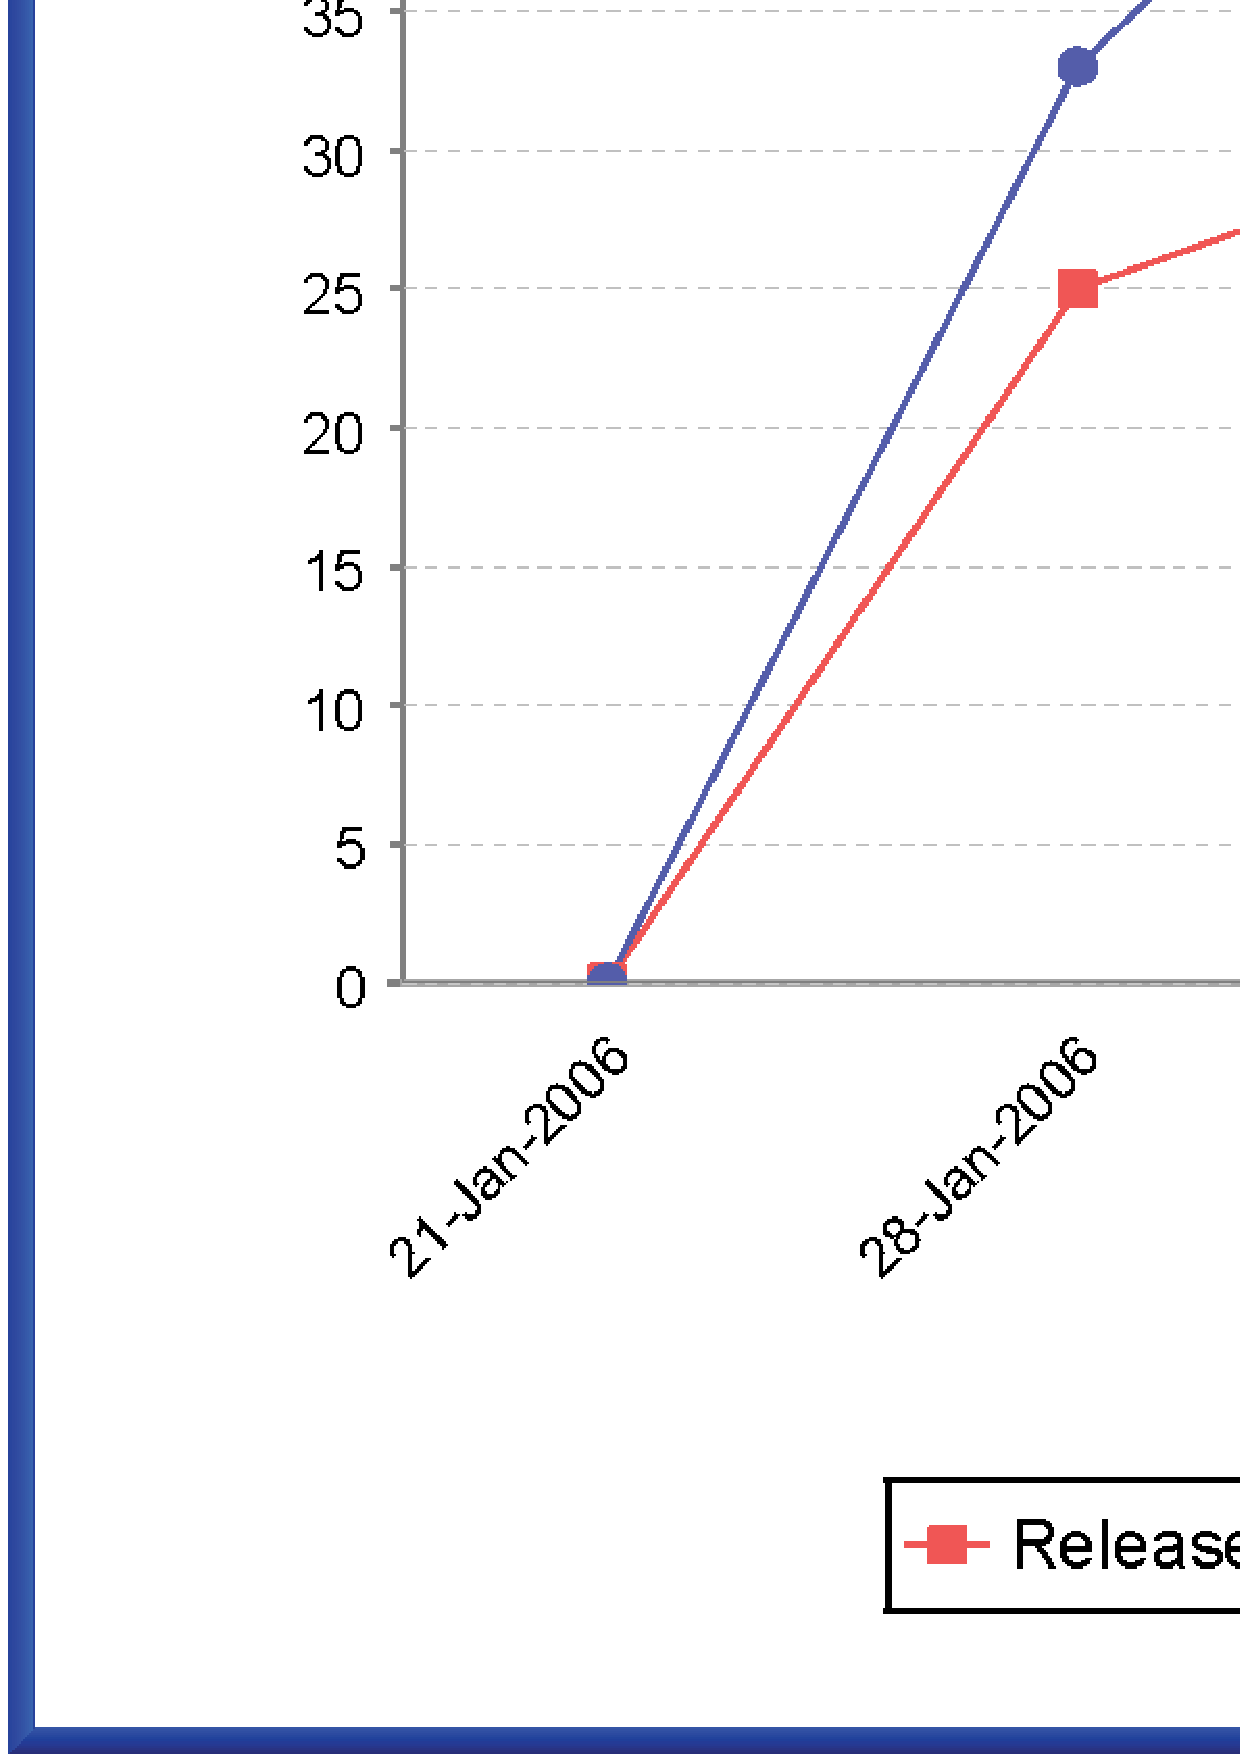
\includegraphics[width=0.70\textwidth]{figures/CSDL-Issue730}
  \caption{Hackystat Release Cycle 7.3 --- Total Issues vs. Remaining Issues} 
  \label{fig:CSDL-Issue730}
\end{figure}

\begin{figure}[p]
  \center
  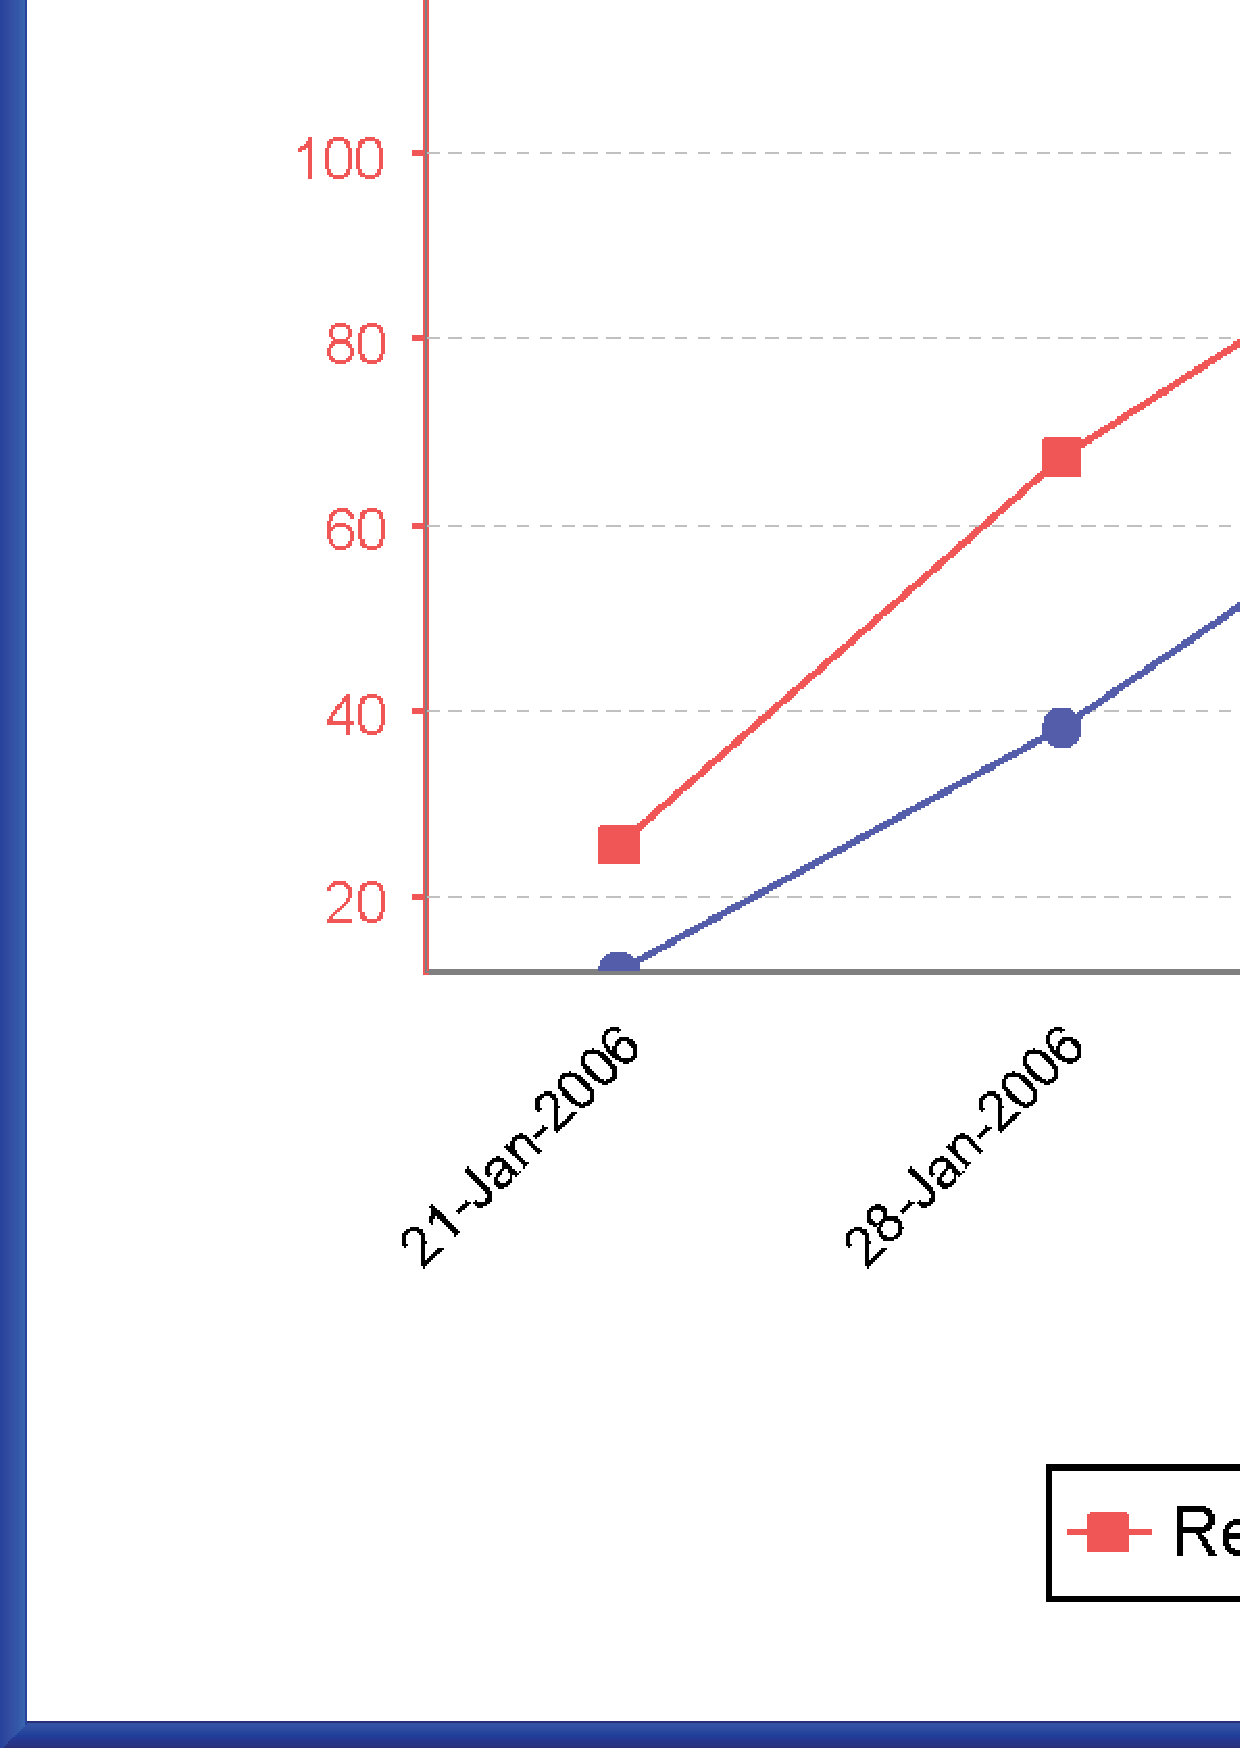
\includegraphics[width=0.70\textwidth]{figures/CSDL-IssueActiveTime730}
  \caption{Hackystat Release Cycle 7.3 --- Total Issues vs. Active Time} 
  \label{fig:CSDL-IssueActiveTime730}
\end{figure}


\begin{figure}[p]
  \center
  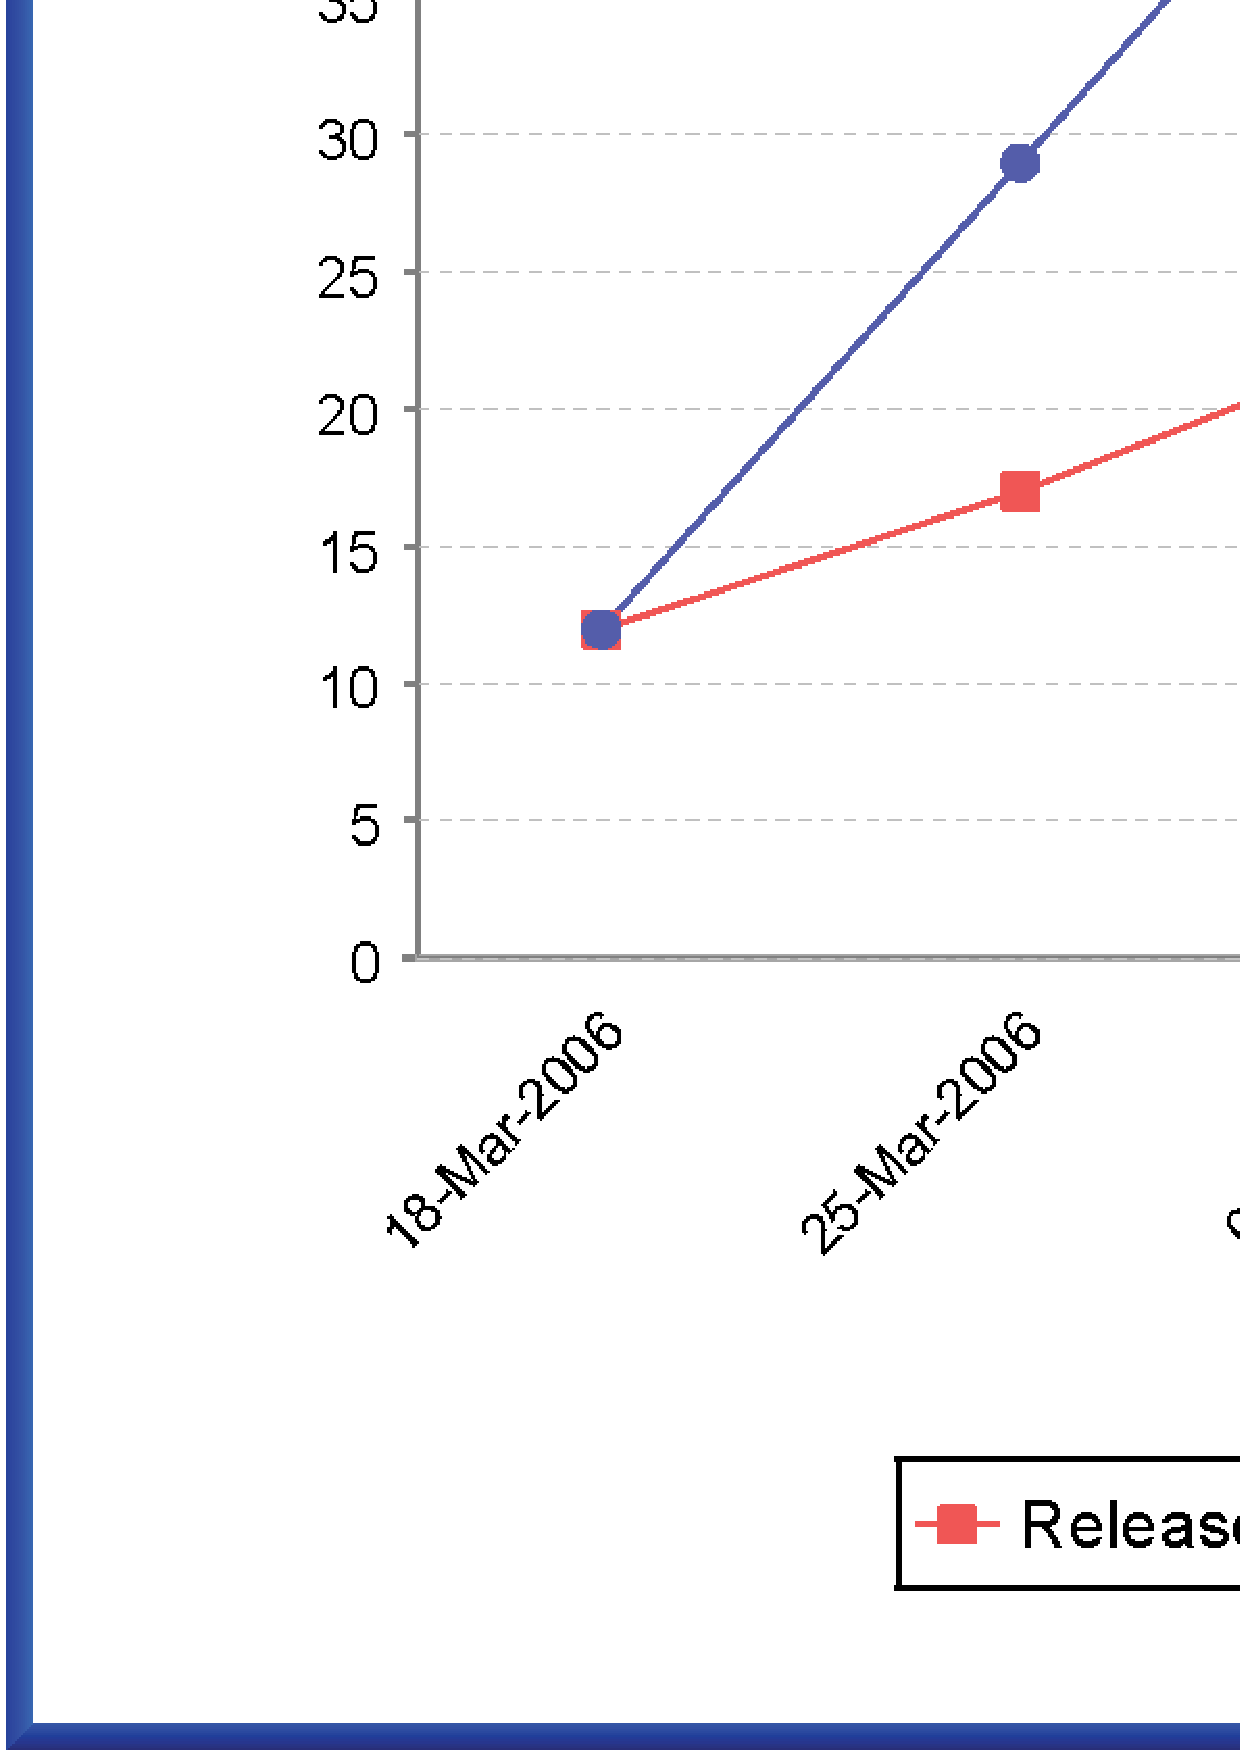
\includegraphics[width=0.70\textwidth]{figures/CSDL-Issue740}
  \caption{Hackystat Release Cycle 7.4 --- Total Issues vs. Remaining Issues} 
  \label{fig:CSDL-Issue740}
\end{figure}

\begin{figure}[p]
  \center
  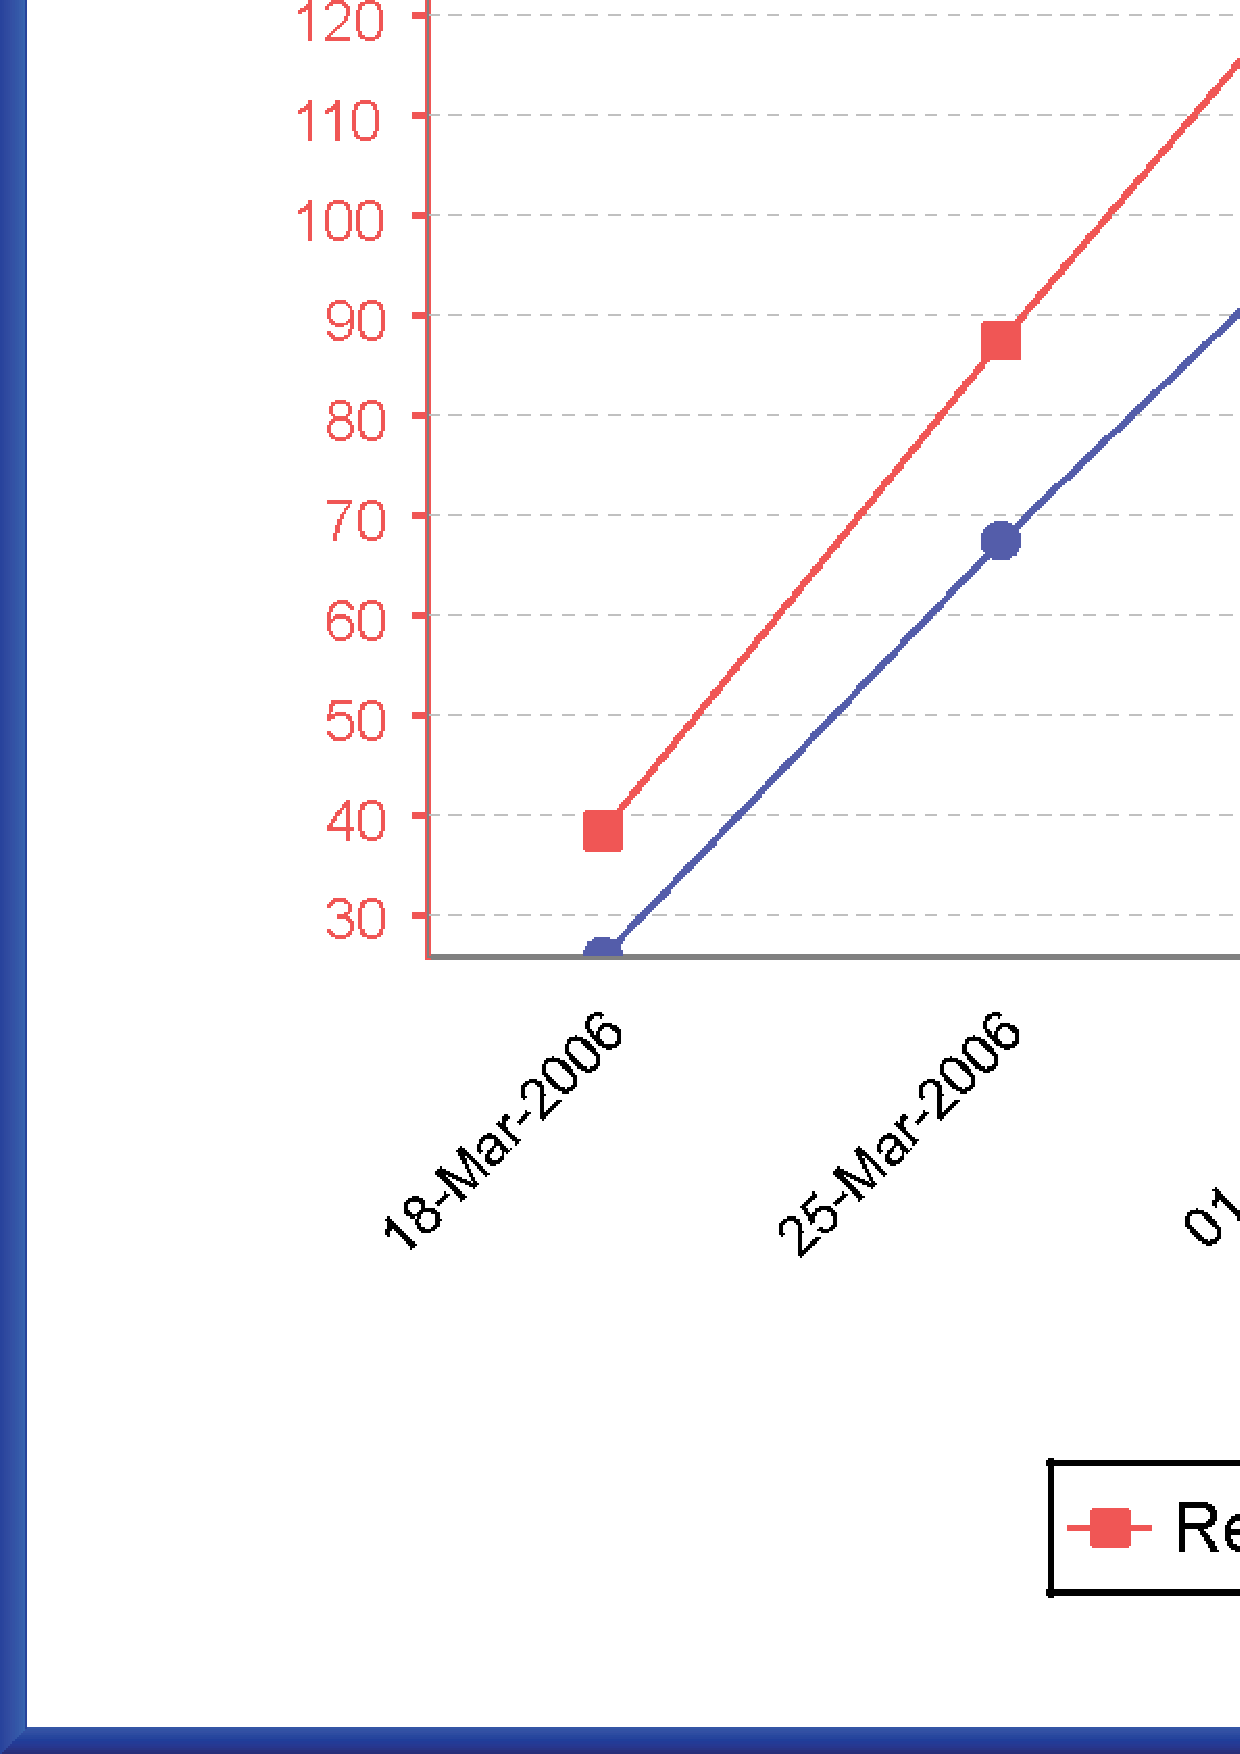
\includegraphics[width=0.70\textwidth]{figures/CSDL-IssueActiveTime740}
  \caption{Hackystat Release Cycle 7.4 --- Total Issues vs. Active Time} 
  \label{fig:CSDL-IssueActiveTime740}
\end{figure}

 









%%%%%%%%%%%%%%%
%  S T O R Y  %
%%%%%%%%%%%%%%%
\clearpage
%\subsection{Software project telemetry helped improve CSDL code quality.}
\subsection{Improvement on CSDL Code Quality}
\label{EvaluationInCSDL:EventsDescription:CodeIssue}

\subsubsection{Pre-hypothesis Data:}
\begin{itemize}
  \setlength{\itemsep}{0pt}
  \setlength{\parskip}{0pt}
  \item 2006-01-09-1: I asked a developer about his perception of the utility of the metrics currently collected in the lab during an interview. He told me that FindBugs reported too many problems, and that a lot of them were false-positive.
  \item 2006-01-11-1: I asked another developer about his perceptions about the utility of the metrics currently collected in the lab. He told me that metrics from FindBugs and PMD were not useful, but they could be made useful if the false-positive problem could be resolved. 
  \item 2006-01-16-1: In the weekly status meeting, the developers commented on the metrics from FindBugs and PMD. They all appeared to agree that there were too many false-positive warnings.
  \item 2006-02-09-2: CSDL deployed FindBugs and PMD sensors, even though the false-positive issue had not been addressed.
  \item 2006-03-23-1: I made the code issue density charts, which were computed from FindBugs and PMD metrics, available on the telemetry wall. I showed the charts to two of the developers. They told me that the charts failed to provide clue about Hackystat code quality, because they did not know the rules used by FindBugs and PMD to generate warnings. 
\end{itemize}

\subsubsection{Generated Hypothesis:}

The FindBugs and PMD warnings would be useful in improving Hackystat code quality, if the false-positive problem could be resolved. Since the development team in CSDL did not have enough resource to examine every single warning, the key to benefit from the tools was to prioritize the warnings they produced. Assuming different types of warnings had different probability of being false-positive, this probability could be used to determine the priority of the warnings.

\subsubsection{Intervention:}

I started with FindBug warnings and categorized them into three groups with different treatment options: \textit{fail}, \textit{monitor}, and \textit{ignore}.

\subsubsection{Post-hypothesis Data:}
\begin{itemize}
  \setlength{\itemsep}{0pt}
  \setlength{\parskip}{0pt}
%  \item 2006-04-17: I conducted a poll before the weekly status meeting. After 3 months FindBug and PMD were deployed, none of the developers had spent over one hour reading the FindBugs and PMD report, which the project manager had only spent 2-3 hours. The number suggested that their opinions were mostly preconceived.
  \item 2006-04-17-3: I discussed with the developers treatment options for each of the 17 types of FindBugs warnings found in hackyCore\_Kernel module in the weekly status meeting. The comments from the developers indicated that they had learned a lot by going over their own code that generated the warnings.
  \item 2006-04-24-1: I discussed with the developers treatment options for the remaining types of FindBugs warnings found in the Hackystat source in the weekly status meeting.
  \item 2006-04-25-1: I modified the code issue telemetry chart to track the number of warnings falling into ``fail'' and ``monitor'' categories.
  \item 2006-04-26-2: The project manager assigned tasks for the developers to get rid of the warnings that fell into the ``fail'' category.
  \item 2006-05-06-1: Telemetry analysis indicated that all the FindBugs warnings in the ``fail'' category had been eliminated, and the warnings in the ``monitor'' category had been reduced by more than a half.
\end{itemize}

\subsubsection{Conclusion:}

The additional data appears to confirm the hypothesis. The intervention was successful. Within two weeks, the developers had completely eliminated the FindBugs warnings in the \textit{``fail''} category, and drove down the FindBugs warnings in the \textit{``monitor''} category by more than a half.

\subsubsection{Elaboration:}

%This subsection reports on a successful experience of how I made \textit{``CodeIssue''} metrics useful as one of the code quality indicators, and helped the developers reduce a significant number of potential buggy code in the \textit{Hackystat} source. 

The \textit{``CodeIssue''} metric is a type of metric designed for representation of problems uncovered by static code analysis tools such as FindBugs\cite{Software:FindBugs} and PMD\cite{Software:PMD}. These tools perform static analysis either on Java source code or compiled byte code, and flag suspicious language constructs, which are potential software bugs. For example, a compiler won't complain if you try to dereference a null pointer, but when executing the code the most probable outcome is application crash.  

In February 2006, CSDL deployed both FindBugs and PMD to run on the Hackystat source. Unlike a compiler where the distinction between bug and non-bug is clear, these static code analyzers can only make probability statements about potential bugs. The general feeling among the developers was that there were too many warnings reported by the tools, and that most of them were false-positive. The telemetry chart in Figure \ref{fig:CSDL-FindBugs-PMD} indicated that in the nine weeks from Feb 25 to April 22, the number of warnings reported by FindBugs had increased from 507 to 518, while the number reported by PMD had increased from 6167 to 6702. The trends looked bad, but nobody was sure whether they constituted proof that the quality of the project had indeed gone down. One developer commented: \textit{``These numbers are potentially useful, but I don't think there are really useful at this time. There are so many false-positives.''} 

My hypothesis was that the warnings reported by FindBugs and PMD contained valuable information to improve Hackystat code quality. Since the development team in CSDL did not have enough resource to examine every single warning, the key to benefit from the tools was to prioritize the warnings they produced. Assuming different types of warnings had different probability of being false-positive, this probability could be used to determine the priority of the warnings.
Based on this hypothesis, I decided to put them into three categories with different treatment options: 

\begin{itemize}
	\item \textbf{Fail} ---- These were the types of warnings with high probability of being true. The existence of such warnings should fail CSDL nightly integration build, so that they could be eliminated immediately after they were detected.
	
	\item \textbf{Monitor} ---- These were the types of warnings with moderate probability of being true. They did not have to be dealt with immediately given the resource constraint faced by CSDL development team. However, the number of these types of warnings should be used as quality indicator and closely monitored for bad trend.

	\item \textbf{Ignore} ---- These were the types of warnings with low probability of being true. The development team should not waste any resource on them.
\end{itemize}

I started with FindBug warnings. For each type of warning, I picked one instance and discussed treatment options with the developers in CSDL weekly meetings. The discussion was overwhelmingly welcomed. The developers told me that they learned a lot about best coding practices to avoid common errors with the samples of warnings generated from their own code.
 
Figure \ref{fig:CSDL-FindBugs} is a telemetry chart showing the number of FindBugs warnings that fell into \textit{``fail''} and \textit{``monitor''} categories respectively. The chart indicated that within two weeks after the discussion, the developers had completely eliminated the warnings in the \textit{``fail''} category, and drove down the number of warnings in the \textit{``monitor''} category by more than a half. The project manager was so happy with the results, that he told me he would follow my approach to do the same thing with PMD warnings after the summer. 

\begin{figure}[p]
  \center
  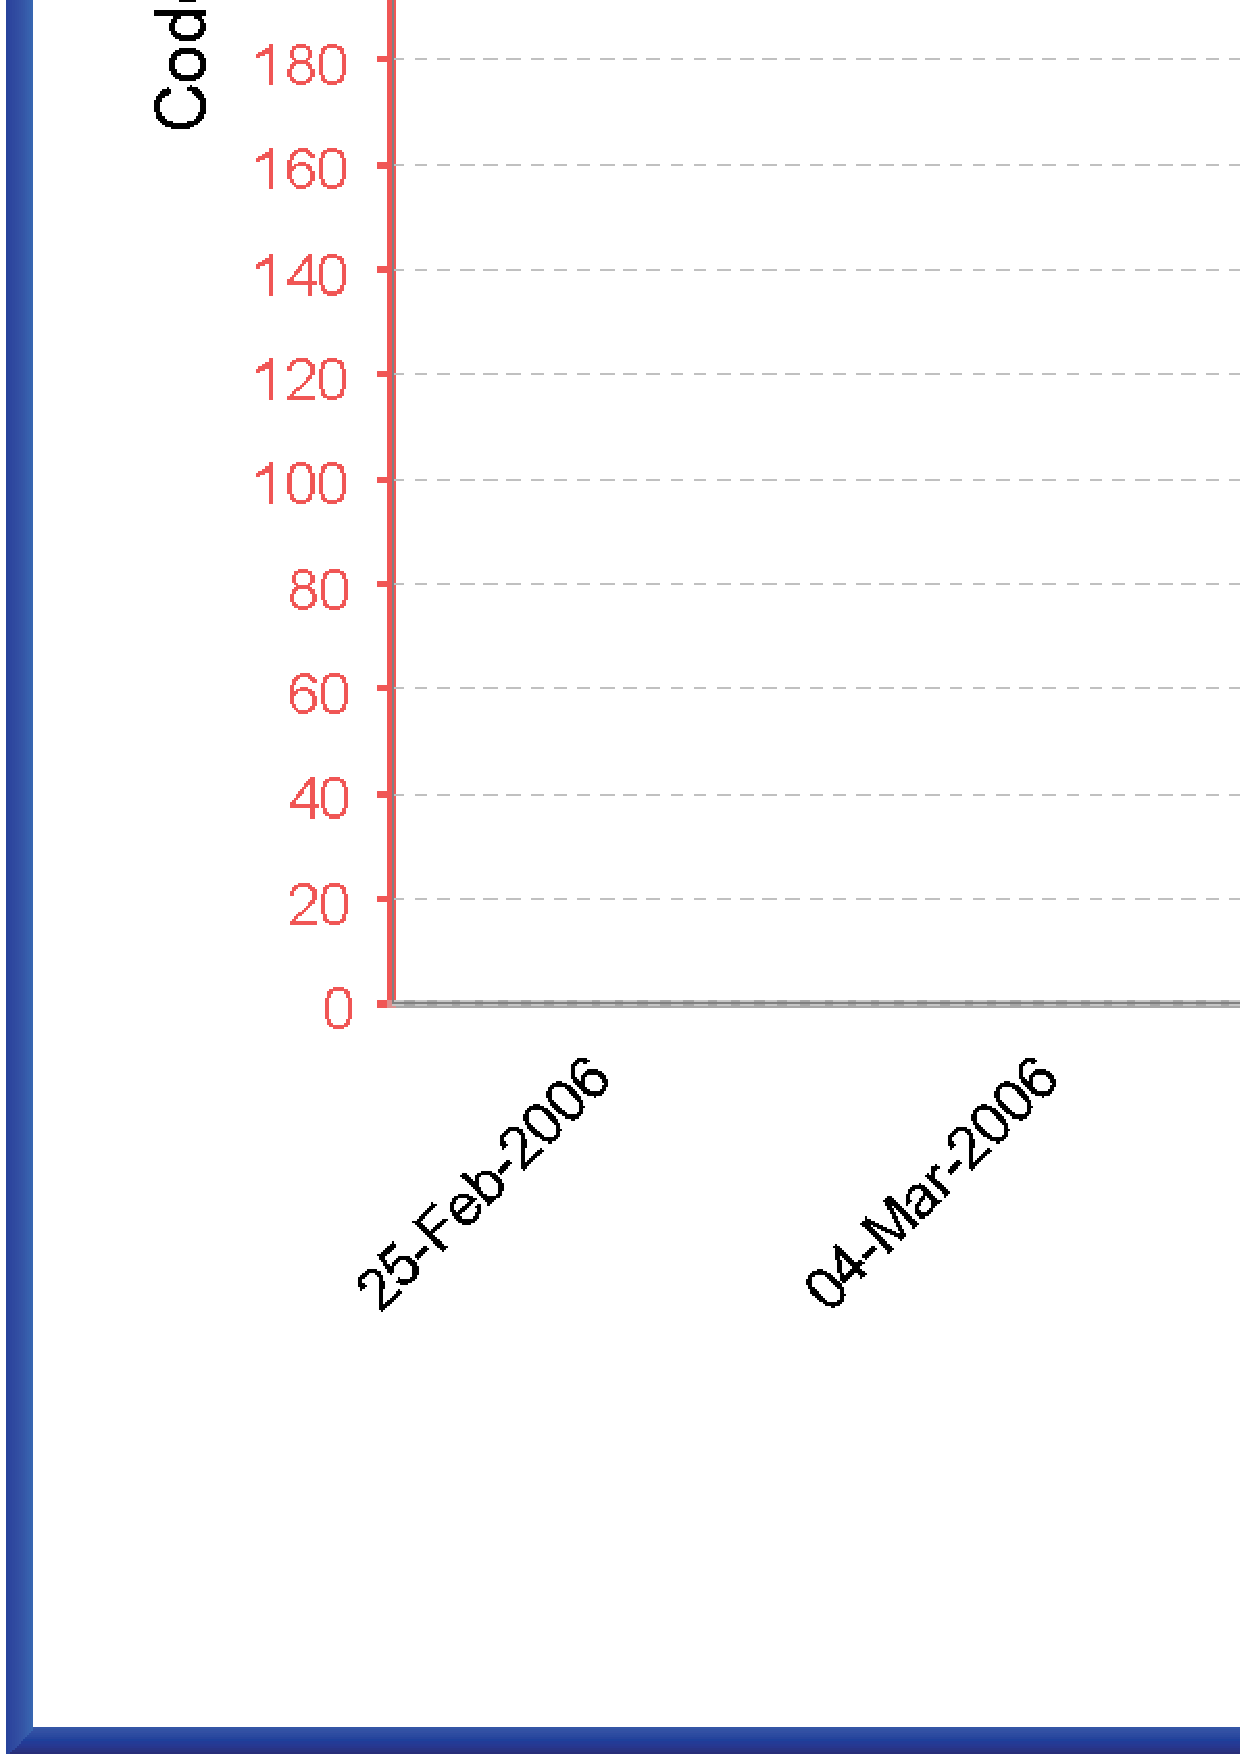
\includegraphics[width=0.70\textwidth]{figures/CSDL-FindBugs-PMD}
  \caption{FindBugs and PMD Warnings from the Hackystat Source} 
  \label{fig:CSDL-FindBugs-PMD}
\end{figure}

\begin{figure}[p]
  \center
  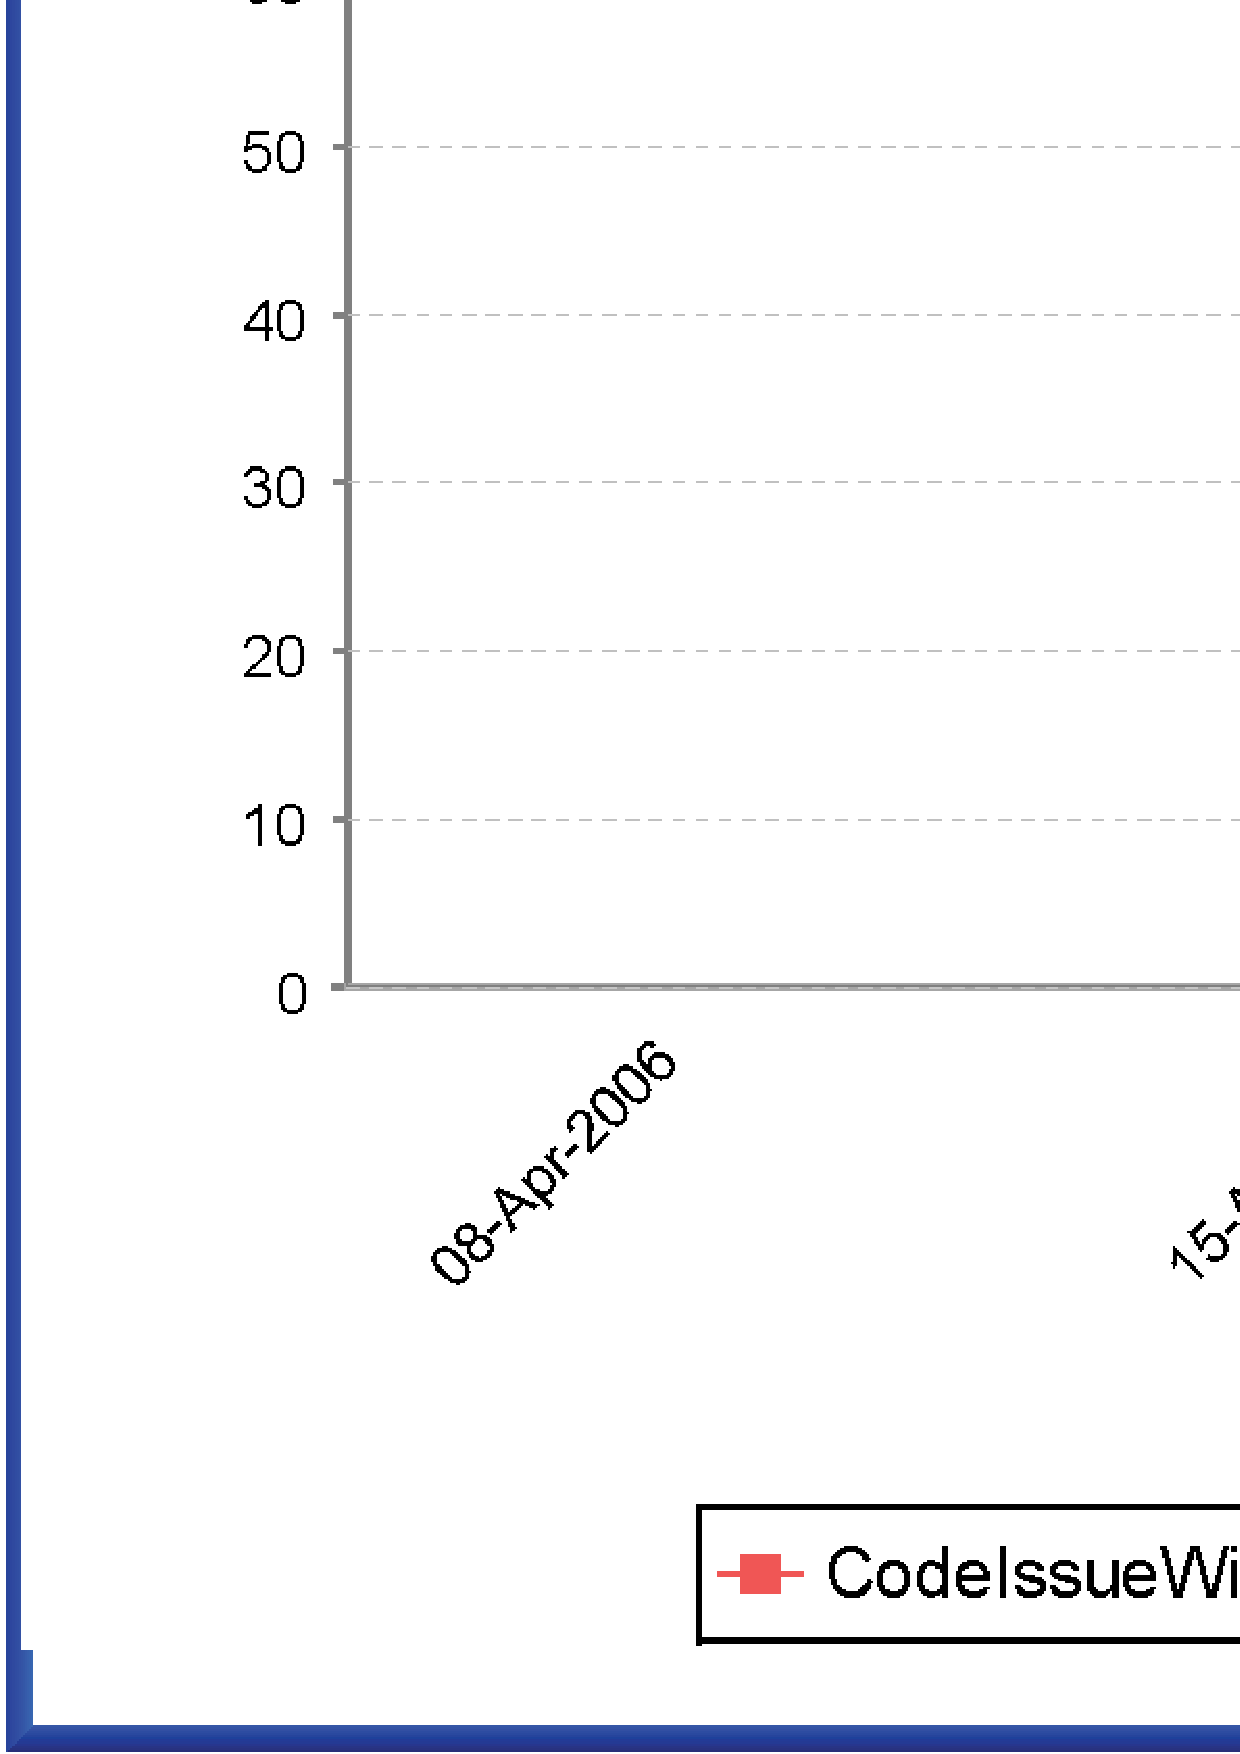
\includegraphics[width=0.70\textwidth]{figures/CSDL-FindBugs}
  \caption{FindBugs Warnings in ``Fail'' and ``Monitor'' Categories} 
  \label{fig:CSDL-FindBugs}
\end{figure}










%%%%%%%%%%%%%%%
%  S T O R Y  %
%%%%%%%%%%%%%%%
\clearpage
%\subsection{Software project telemetry provided the developers with insights into their processes.}
\subsection{Improvement on Developers' Insights into their Software Development Process}
\label{EvaluationInCSDL:EventsDescription:BuildAnalysis}

\subsubsection{Pre-hypothesis Data:}

The pre-hypothesis data came from a previous study in which I analyzed 2004 CSDL integration build failure data. The study found that the build failure rate was significant. The loss of productivity due to the integration build failures was substantial, since each build failure generally required one or more developers to stop concurrent development, diagnose the problem, and determine who was responsible for fixing the error. Often times, other developers had to wait until the corrections were made before they could check out or commit additional code. The study suggested that the causes of the integration build failures were quite complex. They involved at least the following: developer's familiarity with the system, the actual changes made to the code, the dependency relationships among the modules. Since there was no statistical correlation between integration build failures and the number of lines of code committed or the amount of active time spent before the commit, it would be difficult to adopt the traditional approach of building an analytical model to predict the probability of integration build failure in order to forewarn the developers. At the same time, the study also suggested that 74\% -- 82\% of the intergration build failures were preventable if the developers could build and test the system on their workstations before committing the changes to the repository. However, there is a dilemma. On the one hand,  the developers often do not test their changes against the entire code base before committing them, because a full build and test could take over 15-20 minutes, which would be quite time-consuming given that the developers often commit more than once a day. On the other hand, the cost of a broken build is quite time-consuming too, since it could prevent other developers from working when the code repository is in an inconsistent state.

\subsubsection{Generated Hypothesis:}

Software project telemetry could be used to provide feedback to the developers to help them gain insights into their software development processes and the cost associated with integration build failures, so that they could learn from their past experiences to test ``just the right amount'' of the system before committing their changes, where ``just the right amount'' involves a trade-off between local quality assurance effort and increased risk of an integration build failure.
%through making trade-off decisions between reducing local quality assurance effort and reducing integration build failure cost. 

\subsubsection{Intervention:}

Software project telemetry was used to provide process feedback to the developers. To draw their attention, I implemented an email alert that automatically identified the plausible developer responsible for the build failure whenever possible.

\subsubsection{Post-hypothesis Data:}
\begin{itemize}
  \setlength{\itemsep}{0pt}
  \setlength{\parskip}{0pt}
  %\item 2006-01-06: During an interview with a developer, he told me that he did not care about the details of integration build failures unless it was caused by him.
  %\item 2006-01-06: During an interview with another developer, he told me that he did not care about the details of integration build failures unless it was caused by him. 
  %\item A developer break the build, was identified correctly, but blamed others.
  
  \item 2006-01-19-2: I interviewed a developer (developer 1) who was identified as responsible for a recent integration build failure. I asked him how it might impact his local quality assurance practice. He told me that it was \textit{``very effective''} in making him think more about the integration build result when committing changes.%P
  
  \item 2006-01-31-2: I interviewed a developer (developer 2) on the impact of the integration build failure alert mechanism. He commented that it made him \textit{``a little bit more cautious''} when committing changes. %He commented: ``it changed my process a little bit.'' %M
  
  \item 2006-01-31-3: I interviewed developer 1 on the impact of the integration build failure email alert mechanism. He commented: \textit{``you might be identified as a culprit, (which) tends to make you try a little harder to think about when you actually do the thing (i.e., committing changes).''} %P
  
  \item 2006-02-02-3: I interviewed a developer (developer 3) on the impact of the integration build failure alert mechanism. He told me that his behavior was changed significantly from \textit{``I just build the module to see if it works''} to \textit{``I build the entire system and test every time before commit.''} %A
  
  \item 2006-02-02-4: I interviewed a developer (developer 4) on the impact of the integration build failure alert mechanism. He told me that it had not changed his behavior because he was always careful about local quality assurance. %J
  
  \item 2006-03-08-1: I interviewed a developer (developer 5) on the impact of the integration build failure alert mechanism. He told me that he had spent more time on local quality assurance than before. There was overhead, but it was acceptable since it would be much more troublesome to have integration build failures. %H
  
  \item 2006-03-08-2: I interviewed developer 4. He controlled the local quality assurance overhead by reducing the number of commits. %J
  
  \item 2006-03-14-2: I interviewed developer 2. He commented that the overhead on local quality assurance was acceptable give the consequence of integration build failures. He controlled the overhead by reducing the number of commits. %M
  
  %\item 2006-03-22: I provide the project manage a table list all past build failures and asked him to determine which ones are acceptable and which are not. It seemed his criteria also involves trade-off.
  
  \item 2006-03-23-1: I discussed the telemetry charts on integration build failures and various software development process metrics with two of the developers. They confirmed that integration build failure was a complex phenomenon, and that it would be very hard, if not impossible, to predict the probability from the process metrics. 
  
\end{itemize}

\subsubsection{Conclusion:}

The post-hypothesis data appears to confirm the hypothesis. By providing process feedback to the developers, software project telemetry seemed to make them more aware of the cost associated with integration build failures and thus more careful when committing their changes.
Analysis of the developer's process metrics and integration build failure trends (Figure \ref{fig:CSDL-CorrelationAnalysis}) seemed to confirm that they were learning from their past experiences and getting \textit{``smarter''} about their local quality assurance practices.

\subsubsection{Elaboration:}

The Hackystat project is so large that the developers usually work on a subset of the modules relevant to their assignments. An automated integration build tool is used in CSDL to build and test the entire code to make sure that the developers' modifications do not break the system. The process is illustrated in Figure \ref{fig:BuildProcess} and discussed in Section \ref{EvaluationInCSDL:Setting}. 
In early 2005, I conducted a study on CSDL integration build failures using 2004 data. The study suggested that the causes of the integration build failures were quite complex, which involved many factors, such as developer's familiarity with the system, the actual changes made to the code, the dependency relationships among the modules, etc. As a result, I was unable find statistical correlation that could be used describe the causal relationship between software development practices and integration build failures in CSDL.
However, the study did suggest there was a trade-off between developers' local quality assurance effort and integration build failures. Testing the changes against the entire code base before committing them could reduce the integration build failure rate significantly, but it was quite time-consuming. On the other hand, a failed integration build would often waste other developer's time because the code in the repository was in a unsafe state.

My hypothesis in this study was that the phenomena of software development practices and integration build failures are so complex that it would be futile to build a predictive model to describe the causal relationship between them. Instead, software project telemetry could be used to provide feedback to the developers to help them gain insights into their software development processes and the cost associated with integration build failures, so that they could learn from their past experiences to test ``just the right amount'' of the system before committing their changes, where ``just the right amount'' involves a trade-off between local quality assurance effort and increased risk of an integration build failure. In order to draw their attention to telemetry analysis results, I implemented an email alert that automatically identified the plausible developer responsible for the build failure whenever possible.

The data in this study indicated that the result was positive. The responses from the developers (see post-hypothesis data) seemed to suggest that software project telemetry made them more aware of the cost associated with integration build failures. As a result, they seemed to be more careful about committing their changes, and more effort was spent on local quality assurance.

The phenomena resembled the typical textbook case of game theory in Economics. Consider a hypothetical game Adam and Bob are playing, in which each player has two choices: choice 1 and 2. The payoff matrix is listed in Table \ref{table:NashEquilibrium}. Now consider what would happen if Adam and Bob cannot communicate with each other. If Adam's choice is 1, then Bob's best response is 2 because he can get \$110 by choosing 2 instead of \$100 by choosing 1. On the other hand, if Adam's choice is 2, then Bob's best response is still 2 because he can get \$10 by choosing 2 instead of \$0 by choosing 1. In other words, Bob's best response is always 2 regardless of Adam's choice. If you apply the same logic to Adam, then you would find that Adam's best response is always 2 regardless of Bob's choice. Therefore, both Adam and Bob would end up with \$10 when they cannot communicate with each other, and thus cannot reach a mutually beneficial deal.\footnote{This is what is called Nash equilibrium in Economics. A much more complex version of it is often used to model market outcome in a duopoly competition.} Both players act rationally trying to maximize his own benefit. However, obviously, rational decisions are not always optimal, because if Adam and Bob could reach a binding agreement, then both of them would end up much better off by getting \$100 each. 

\begin{table}[tbp]
	\centering
		\caption{Nash Equilibrium in a Non-Cooperative Game}
		\begin{tabular}{|p{0.20\textwidth}|p{0.20\textwidth}|p{0.18\textwidth}|} 
			\hline
			{} & \textbf{Bob Choosing 1} & \textbf{Bob Choosing 2} \\
			\hline
			\textbf{Adam Choosing 1} & -- Adam gets \$100; -- Bob gets \$100. & -- Adam gets \$0 ; -- Bob gets \$110. 
			\\
			\hline
			\textbf{Adam Choosing 2} & -- Adam gets \$110; -- Bob gets \$0. & -- Adam gets \$10; -- Bob gets \$10. 
			\\
			\hline
		\end{tabular}
	\label{table:NashEquilibrium}
\end{table}

Put it in the context of CSDL, I can hypothesize that the developers were always making rational decisions to reduce their software development effort. Before the introduction of software project telemetry, they were less aware of the productivity loss of the integration build failures incurred by other developers, and their decisions were more or less focused on minimizing local quality assurance effort. As a result, they ended up in the low payoff position. On the other hand, the process feedback mechanism I introduced with software project telemetry made them more aware of the cost associated with the integration build failures, and they began to make trade-off decisions to minimize the total combined cost instead of only local quality assurance cost. As a result, though the local quality assurance effort as experienced by individual developers had increased, the entire team were actually moving toward the high payoff position. 

Figure \ref{fig:CSDL-CorrelationAnalysis} provides evidence that the developers were learning to make trade-off decisions between reducing local quality assurance cost and reducing integration build failure cost in order to minimize the total cost.
The first chart shows the number of integration build failures in each month from January to April 2006. 
The second chart shows the number of times that the build script was invoked by the developers on their workstations. A typical purpose was to test the modifications locally before committing them to the repository.
The last chart showed three telemetry streams on \textit{FileCommit}, \textit{CodeChurn}, and \textit{ActiveTime}. \textit{FileCommit} measures the total number of files in all commits from all developers. \textit{CodeChurn} is related to file commit. It computes the total number of lines added and deleted in each revision. \textit{ActiveTime} computes the amount of time a developer spent actively editing code inside an IDE. They all measure software development effort except from different angles.

It seemed that the developers were learning from their past experiences and getting \textit{``smarter''} about their processes. January was the month with low development effort, large amount of local testing, and low integration build failures. It seemed to suggest that low integration build failure was achieved at the cost of lots of local tests. In February, development effort went up with no significant change in local testing pattern, resulting in higher number of integration build failures. March was the month with high development effort, moderate integration build failure rate, and very low local testing effort. This seemed to support the hypothesis that the developers had learned from their past experiences to test ``just the right amount'' of the system before committing their changes.

On a cursory look, the April data seemed contradictory to that hypothesis, with extremely high rate of integration build failure. But further investigation indicated that the April data were not directly comparable. April was the time that CSDL embarked on a completely different type of software development task: the team were busy with updating the Hackystat infrastructure code to support sensor data type evolution. The integration build failures concentrated on several non-actively-maintained leaf modules that were not in the developers' working set. They were exactly the type of build failures the integration build system was designed to detect. My CSDL study ended in early May, but I can conjecture that with continued metrics collection, I would find evidence that the developers are beginning to learn to deal with the new situation and bringing integration build failure back under control. 

\begin{figure}[p]
  \center
  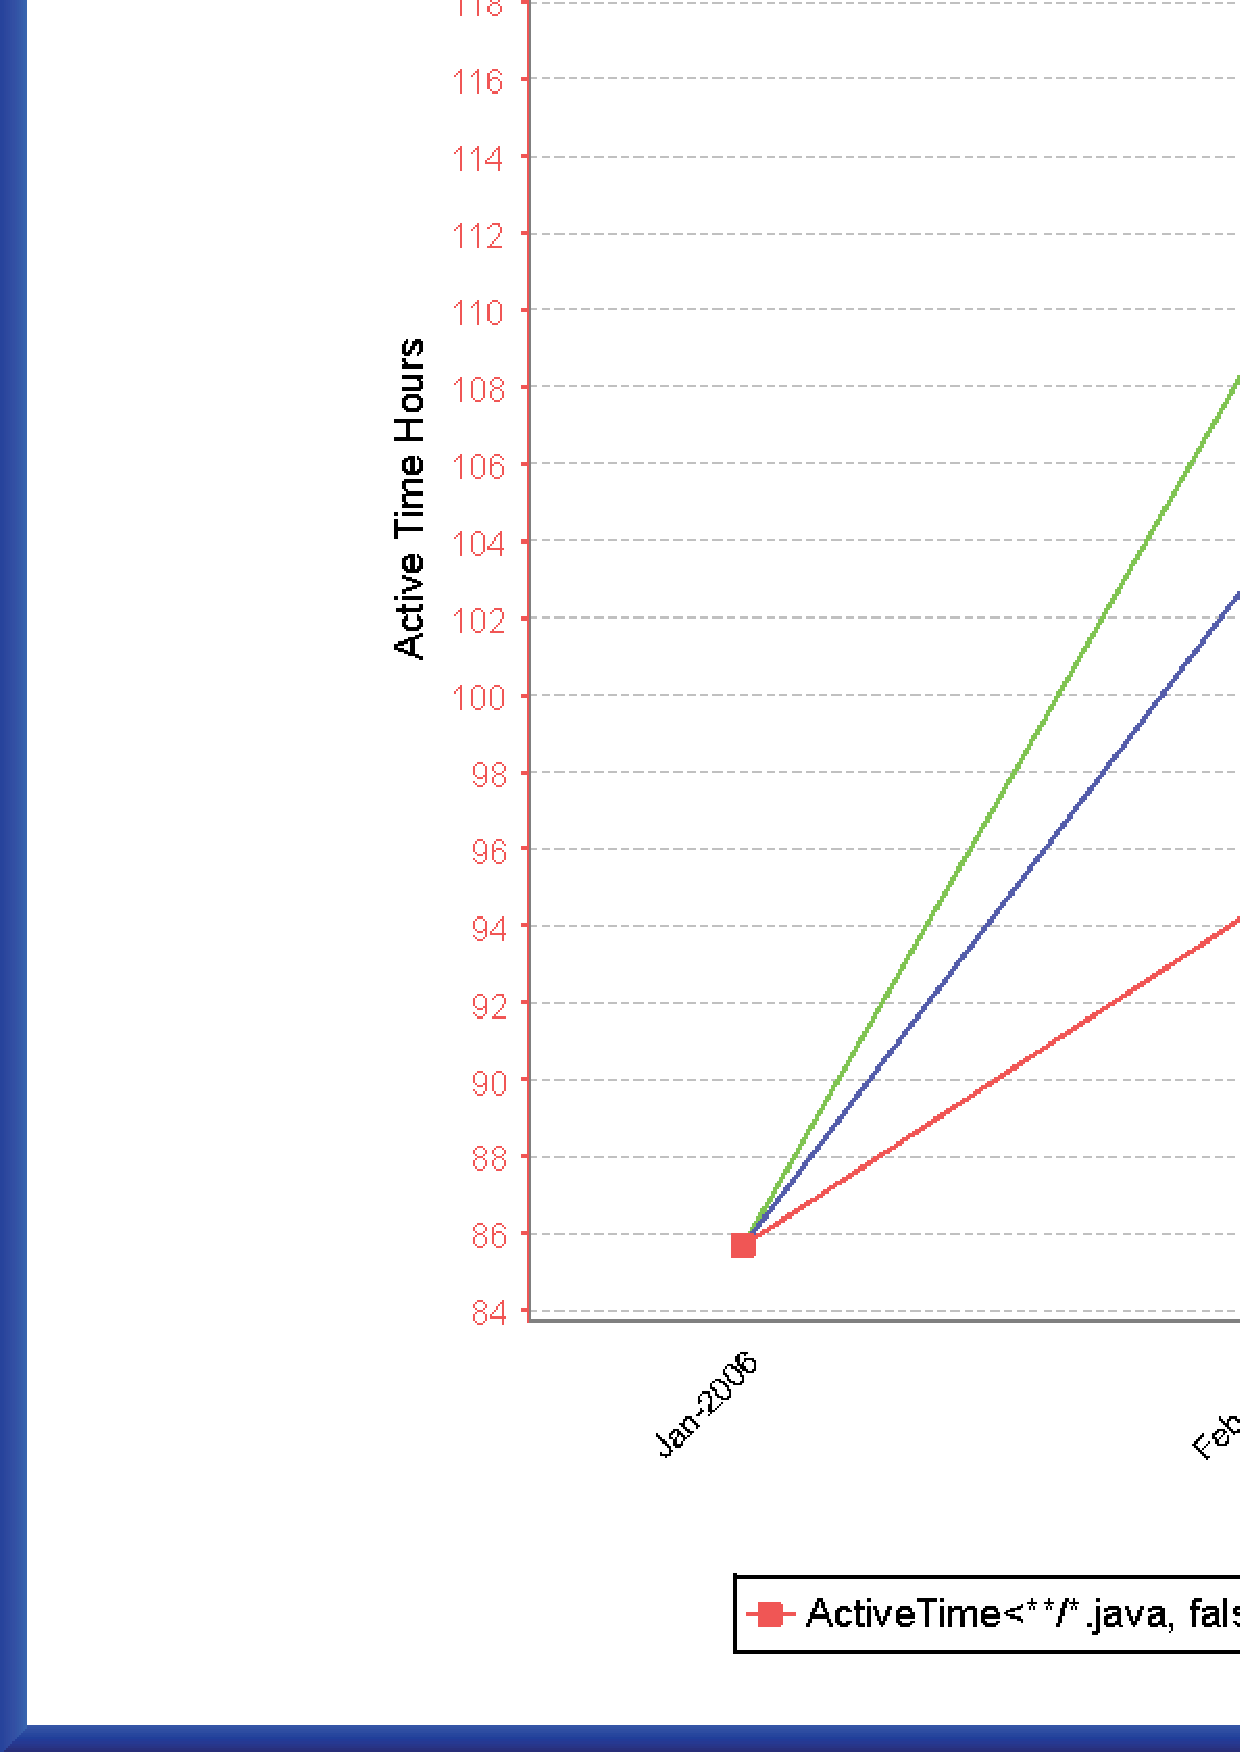
\includegraphics[width=0.67\textwidth]{figures/CSDL-CorrelationAnalysis}
  \caption{Integration Build Failures and Process Metrics} 
  \label{fig:CSDL-CorrelationAnalysis}
\end{figure}












%%%%%%%%%%%%%%%
%  S T O R Y  %
%%%%%%%%%%%%%%%
\clearpage
%\subsection{Top-down telemetry design is a best practice.}
\subsection{Top-down Telemetry Design}
\label{EvaluationInCSDL:EventsDescription:TopDownDesign}

\subsubsection{Pre-hypothesis Data:}
\begin{itemize}
  \setlength{\itemsep}{0pt}
  \setlength{\parskip}{0pt}
  \item 2006-01-16-1: In a weekly status meeting, the developers noted that one could generate a lot of telemetry charts using the telemetry language. But they also asked: \textit{``do we really care about all those charts?''}
  %\item 2006-02-01: \textcolor{red}{The project manager sent me an email regarding what he wishes to see on the telemetry wall.}
	\item 2006-02-05-1: I gathered a list of the types of metrics collected in CSDL, and generated telemetry charts to show how these metrics changed over time in different grain size. The telemetry wall was up.
	\item 2006-02-06-1: I introduced the telemetry wall in the weekly status meeting, but the project manager and the developers found that most of the charts were not useful, except the release cycle issue tracking charts. They gave me a list of questions that they wished telemetry charts could help shed light on, such as some notion of quality indicators for each module in the project.
\end{itemize}

\subsubsection{Generated Hypothesis:}
The telemetry charts generated in a bottom-up fashion (i.e., organized by the types of metrics) were generally not useful, because they were not designed with any purpose in mind. You cannot expect the project manager or the developers to fish around hundreds of charts to find the ones that are useful to them. The reason that the issue tracking charts were found useful was because they happened to have a purpose: allowing the manager to track progress in a release cycle. Therefore, useful telemetry charts are those that are designed with a specific top-level goal in mind.

\subsubsection{Intervention:}
I redesigned the telemetry charts for the telemetry wall, organizing them by their intended use (i.e., top-down design). For example, there was a scene (a set of related charts displayed together on the telemetry wall) for release cycle issue tracking, and there was another scene for module level quality indication.

\subsubsection{Post-hypothesis Data:}
\begin{itemize}
  \setlength{\itemsep}{0pt}
  \setlength{\parskip}{0pt}
  \item 2006-02-21-2: I discussed the top-down designed charts with three of the developers, and they thought the charts displayed useful information.
	\item 2006-02-22-1: I showed the charts to the project manager, and he liked them.
	\item 2006-03-07-1: After receiving complaints about missing coverage data, the project manager sent me an email asking whether it would be possible to design charts to help detect sensor malfunction.	
	\item 2006-03-09-1: A set of charts specifically designed for the purpose of verifying developer-side process metrics were deployed on the telemetry wall. Immediately, I noticed that one of the developers had missing data. It turned out that the developer reinstalled the IDE but forgot to reattach the sensor.
	\item 2006-03-17-1: The project manager was so impressed with the utility of those top-down designed telemetry charts on the telemetry wall, that he decided to devote an entire page on the Hackystat website to publish the results.
\end{itemize}

\subsubsection{Conclusion:}
The additional data appears to confirm the hypothesis. Though \textit{``bottom-up telemetry design''} based on the types of metrics can generate hundreds of charts without significant effort, the charts lack clear purposes and are generally of little value to users. \textit{``Top-down telemetry design''} based on user goals, which is similar to the idea in the Goal-Question-Metric paradigm, yields useful telemetry charts.

\subsubsection{Elaboration:}

At the beginning of this study, I used bottom-up approach to generate telemetry charts to be displayed on the telemetry wall. I gathered a list of the types of metrics collected in CSDL, and then generated charts to show how these metrics change over time in different grain sizes with possible breakdown to individual developer or individual source code module. The charts were organized by the types of metrics. For example, a scene on the telemetry wall might be displaying charts all related to \textit{active time}, and another scene might be displaying charts all related to \textit{code issue} density.

With the bottom-up approach, hundreds of charts could be easily generated. I introduced them in a weekly status meeting. However, I found that most of them were not useful. 
A frequent question the project manager and the developers asked during my presentation was: \textit{``Why would that be of use to me?''} The only exception was the charts related to release cycle issue tracking, which the project manager found \textit{``highly useful.''}
Further discussion revealed that the project manager and the developers had a number of questions they wished software project telemetry could shed light on, such as:
\begin{itemize}
	\item \textit{``Could telemetry help me identify the situation where the sensors are likely not being installed?''}
	\item \textit{``Could telemetry offer some notion of quality so that it helps me locate the modules with low quality, or the modules that are changing with respect to quality?''}
	\item \textit{``Could telemetry give me a sense of how we are making progress toward the stable release?''}
\end{itemize}

My hypothesis was that bottom-up telemetry design was unsuccessful because it generated hundreds of charts organized by metrics types. You just cannot expect users to go over all those charts to find the ones that are useful to them. The issue tracking charts were useful because they happened to serve a purpose: they enabled the project manager to track progress in a release cycle. In order for other charts to be useful, they have to be re-organized in a top-down fashion by the questions they intended to answer. 
%\textcolor{red}{In fact, the project manager already state what he wished to see. 2006-02-01. I did not pick up the hint, and continued to use bottom-up approach.}
Based on this hypothesis, I redesigned the telemetry charts following top-down approach, which resulted in a number of successful telemetry scenes being displayed on the telemetry wall:

\begin{itemize}
  \setlength{\itemsep}{0pt}
  \setlength{\parskip}{0pt}
	\item A telemetry scene for release cycle issue tracking.
  \item A telemetry scene for product metrics at project level for quality indication.
  \item A set of telemetry scenes for product metrics at module level for quality indication. One scene per module.
  \item A telemetry scene for module filtering to discover interesting information in a large project like \textit{Hackystat}.
  \item A telemetry scene for software development process metrics and correlation analysis.
  \item A telemetry scene for sensor data verification.
\end{itemize}

The top-down designed telemetry charts were so successful that the project manager decided to devoted an entire page on Hackystat website to publish the results. A snapshot is captured in Figure \ref{figures/TelemetryReport-Page1} and \ref{figures/TelemetryReport-Page2}. The URL of the web page is:
\begin{quotation}
	\textit{http://www.hackystat.org/hackyDevSite/telemetryReport.do}
\end{quotation}

The web page contains a collection of both \textit{historical} and \textit{real-time} charts, which serves two purposes: 
(1) enabling the entire Hackystat developer community, especially those off-site developers, to monitor the project development status, and (2) demonstrating the power of the Hackystat framework by showing the achievement of one of its extensions.

\begin{figure}[p]
  \center
  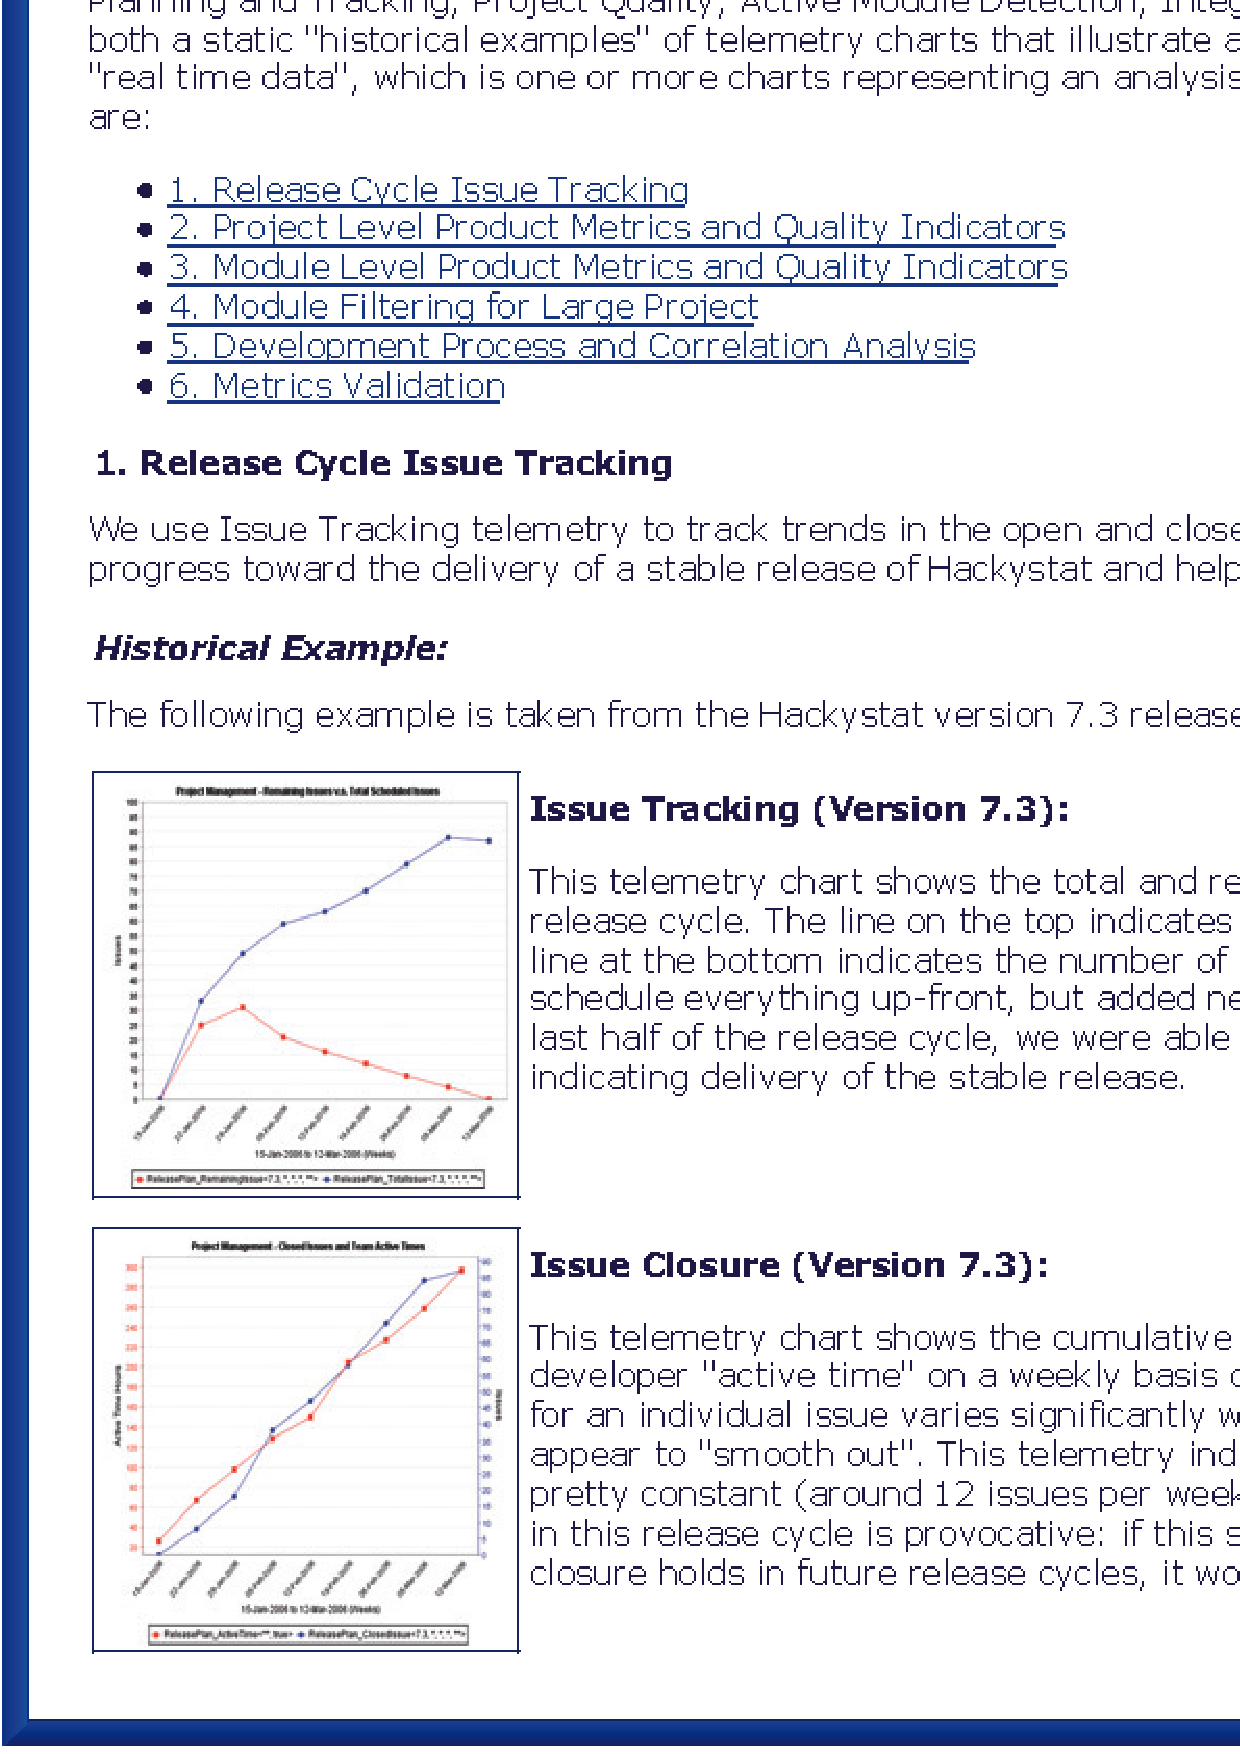
\includegraphics[height=0.93\textheight]{figures/TelemetryReport-Page1}
  \caption{Telemetry Report: Page 1} 
  \label{figures/TelemetryReport-Page1}
\end{figure}

\begin{figure}[p]
  \center
  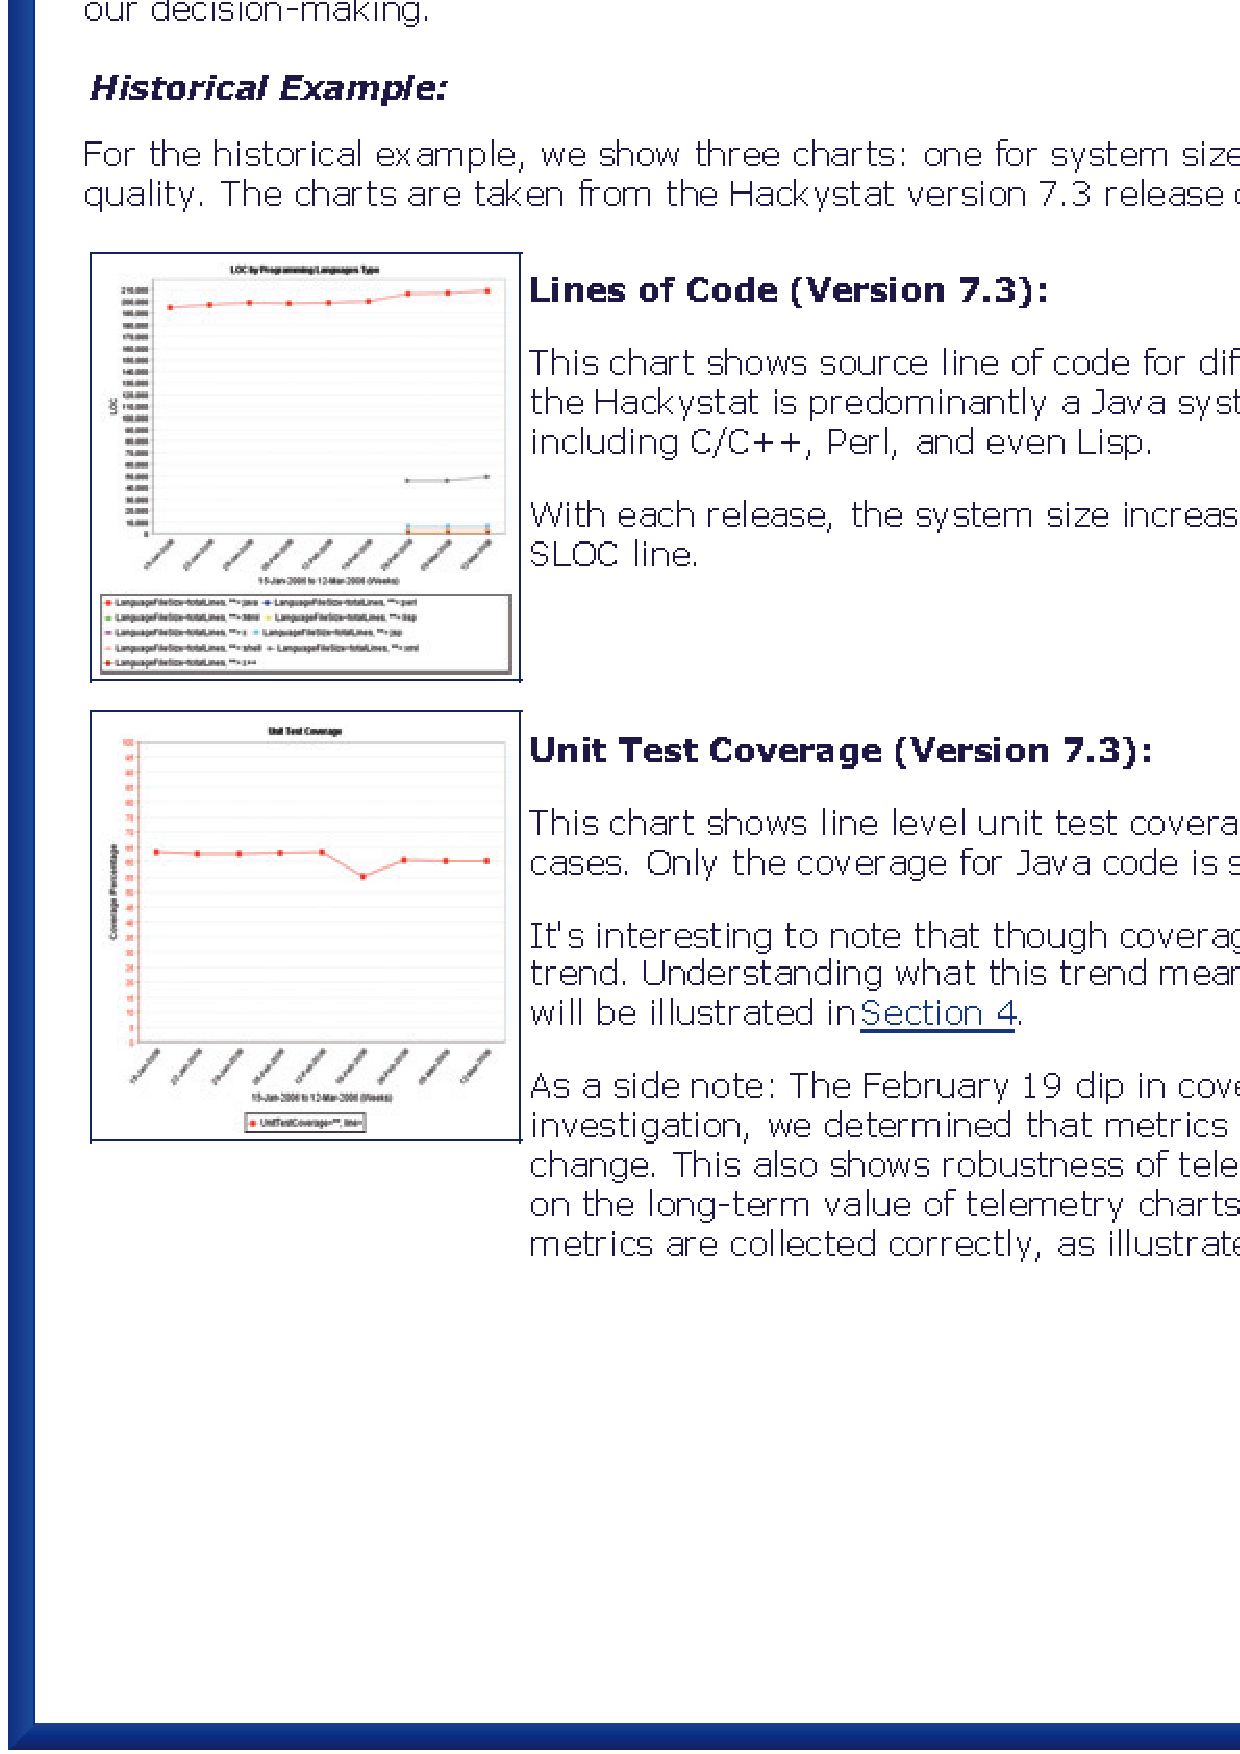
\includegraphics[height=0.93\textheight]{figures/TelemetryReport-Page2}
  \caption{Telemetry Report: Page 2} 
  \label{figures/TelemetryReport-Page2}
\end{figure}








%%%%%%%%%%%%%%%
%  S T O R Y  %
%%%%%%%%%%%%%%%
\clearpage
%\subsection{Using software project telemetry for sensor data self-verification is a best practice.}
\subsection{Sensor Verification}
\label{EvaluationInCSDL:EventsDescription:DataVerification}

\subsubsection{Pre-hypothesis Data:}
\begin{itemize}
  \setlength{\itemsep}{0pt}
  \setlength{\parskip}{0pt}
  \item 2006-01-31-4: I noticed an inconsistency in telemetry charts: there was no data from one of the developers. It turned out it was caused by a bad server-side project configuration.
  \item 2006-02-01-1: The same developer told me he had fixed the problem, but the inconsistency still existed in telemetry charts. The project was still mis-configured despite the developer's effort to fix it.
  \item 2006-02-06-1: During my presentation of telemetry charts in the weekly status meeting, I noticed that the developers were using some of the charts to assess whether the underlying sensors data seemed correct or not. Further discussion identified two common causes for incorrect sensor data: (1) sensor not working correctly, and (2) bad server-side project configuration.
\end{itemize}

\subsubsection{Generated Hypothesis:}

There is always possibility for incorrect sensor data. Ensuring sensor data correctness is a tedious and time-consuming process, because a developer has to log onto the server to compare raw sensor data entries with his expectations. Specially designed telemetry charts could save much of the effort by allowing a developer to make quick assessment of the likelihood of occurrence of sensor data problem.

\subsubsection{Intervention:}

I designed a set of sensor data verification charts, and made them available both on the telemetry wall and on the public Hackystat website.

\subsubsection{Post-hypothesis Data:}
\begin{itemize}
  \setlength{\itemsep}{0pt}
  \setlength{\parskip}{0pt}
  \item 2006-02-26-1: Telemetry charts showed missing coverage data. It turned out that the sensor configuration file was not updated when a developer added a new module.
  \item 2006-03-05-1: Telemetry charts showed missing issue metrics. It turned out that a developer forgot to update the project configuration when adding a new module.
  \item 2006-03-09-1: I added additional telemetry charts on the telemetry wall, designed to verify developer-side process metrics. Immediately, I detected that one developer has missing active time data. It turned out that the developer reinstalled the IDE but forgot to reattach the sensor.
  \item 2006-04-20-1: A developer modified Jira sensor code. Telemetry charts showed missing issue metrics. It turned out it was caused by a bug in the code.
  \item 2006-04-22-2: An email from the project manager indicated he detected the same Jira sensor problem using the real-time sensor verification charts on the public Hackystat website.    
\end{itemize}

\subsubsection{Conclusion:}

The data appears to suggest that it would be hard to avoid sensor data problem. The problem was most severe when a project's scope was changed, such as adding a new module. Nevertheless, specially designed telemetry charts are efficient at detecting the problem. It seems that the best practice would be to designate a person to spend one or two minutes each day to examine the charts for early detection of sensor data problem. 


\subsubsection{Elaboration:}

The central idea of sensor-based metrics collection is that sensors are designed to collect metrics automatically and unobtrusively. Once they are installed, they work silently in the background. It is very easy for a developer to forget about the existence of the sensors. At the same time, it also means that sensor data problem can go unnoticed for a long time. Bad sensor data are caused by many reasons, such as software bug, inappropriate sensor configuration, and server-side project configuration. Though telemetry analysis has greater tolerance for incorrect metrics compared to traditional model-based metrics approaches, complete and correct data still provide the best decision-making value. However, ensuring sensor data correctness is a tedious task. A developer has to log onto the server where raw sensor data are stored and compare the entries with his expectations. It typically involves thousands of sensor data entries on a project of the size like Hackystat.

A serendipitous discovery in this study was that there were several instances that inconsistencies in telemetry charts helped detect the underlying sensor data problem. 
My hypothesis was that these were not isolated events and that it was possible design telemetry charts to allow the developers to make quick assessment of the likelihood of the occurrence of sensor data problem. These charts could be used in a number of different ways:

\begin{itemize}
	\item \textbf{Detecting dropout of data points in telemetry streams:}

A dropout usually indicates that the sensor did not send the data. For some types of metrics, it is completely normal. For example, \textit{ActiveTime} is only generated when a developer is actively editing code inside an IDE. It is normal for it drop out for a few days because the developer might be taking a break. But a dropout of \textit{ActiveTime} for a prolonged period of time might be indicative of problem. For other types of metrics, any dropout signifies an error condition. For example, CSDL uses an integration build system to run unit tests and collect coverage metrics every night automatically. There should be no missing data point in coverage data stream if everything is working as expected.

	\item \textbf{Detecting outliers or sudden value changes in telemetry streams:}
	
An outlier or sudden value change is normal if it is caused by drastic change in software development process or software product. But, often times, it is an indication of sensor breakdown: sending incomplete or incorrect data to the server.

	\item \textbf{Detecting whether related metrics were changing together or not:}

Some related metrics should change together with each other. For example, in Figure	\ref{fig:CSDL-DeveloperSensorVerification}, active \textit{time}, \textit{build}, \textit{unit test}, and \textit{commit} are related because they all serve as proxy for software development effort. If one of them does not co-vary with the rest, it usually indicates that the sensor is not working correctly.
	
\end{itemize}

After I made the sensor data verification telemetry charts available, they supported early detection of several instances of sensor data problems. 
One instance involved Figure \ref{fig:CSDL-CoverageSensorVerification}, which showed a chart tracking unit test coverage. The chart was generated for the period from Feb 14 to Feb 26 on a daily interval. There was no unit test data after Feb 20. The sudden drop of coverage from 64\% to 55\% made it even more suspicious that something significant had occurred to the project around that day which broke the \textit{Emma} sensor.\footnote{\textit{``Emma''} sensor was the sensor CSDL used to collect unit test coverage information.} Further investigation revealed that one of the developers had created a new module, but forgot to update the configuration file to include that  module.

Another instance involved Figure \ref{fig:CSDL-DeveloperSensorVerification}, which showed a chart representing four types of metrics related to software development effort: the number of active time hours, the number of local builds, the number of unit test invocations, and the number of commits. The four types of metrics should all co-vary with each other, because they all represent software development effort albeit from different perspectives. For example, from Feb 16 to Mar 6, everything was normal. When active time was high, the other three types of metrics were high. When active time was low, the other three types of metrics were low. When active time was zero, the other three types of metrics were zero too. However, for the four days from Mar 7 to Mar 10, the metrics values were abnormal. The developer had build, unit test, and commit activities, but there was no active time. Further investigation revealed that the developer had reinstalled Eclipse IDE, but forgot to reattach the sensor.

The CSDL experience appears to suggest that it is almost impossible to avoid sensor data problem altogether, the best practice would be to designate a person to spend one or two minutes each day to examine the charts for early detection of sensor data problem. 

\begin{figure}[p]
  \center
  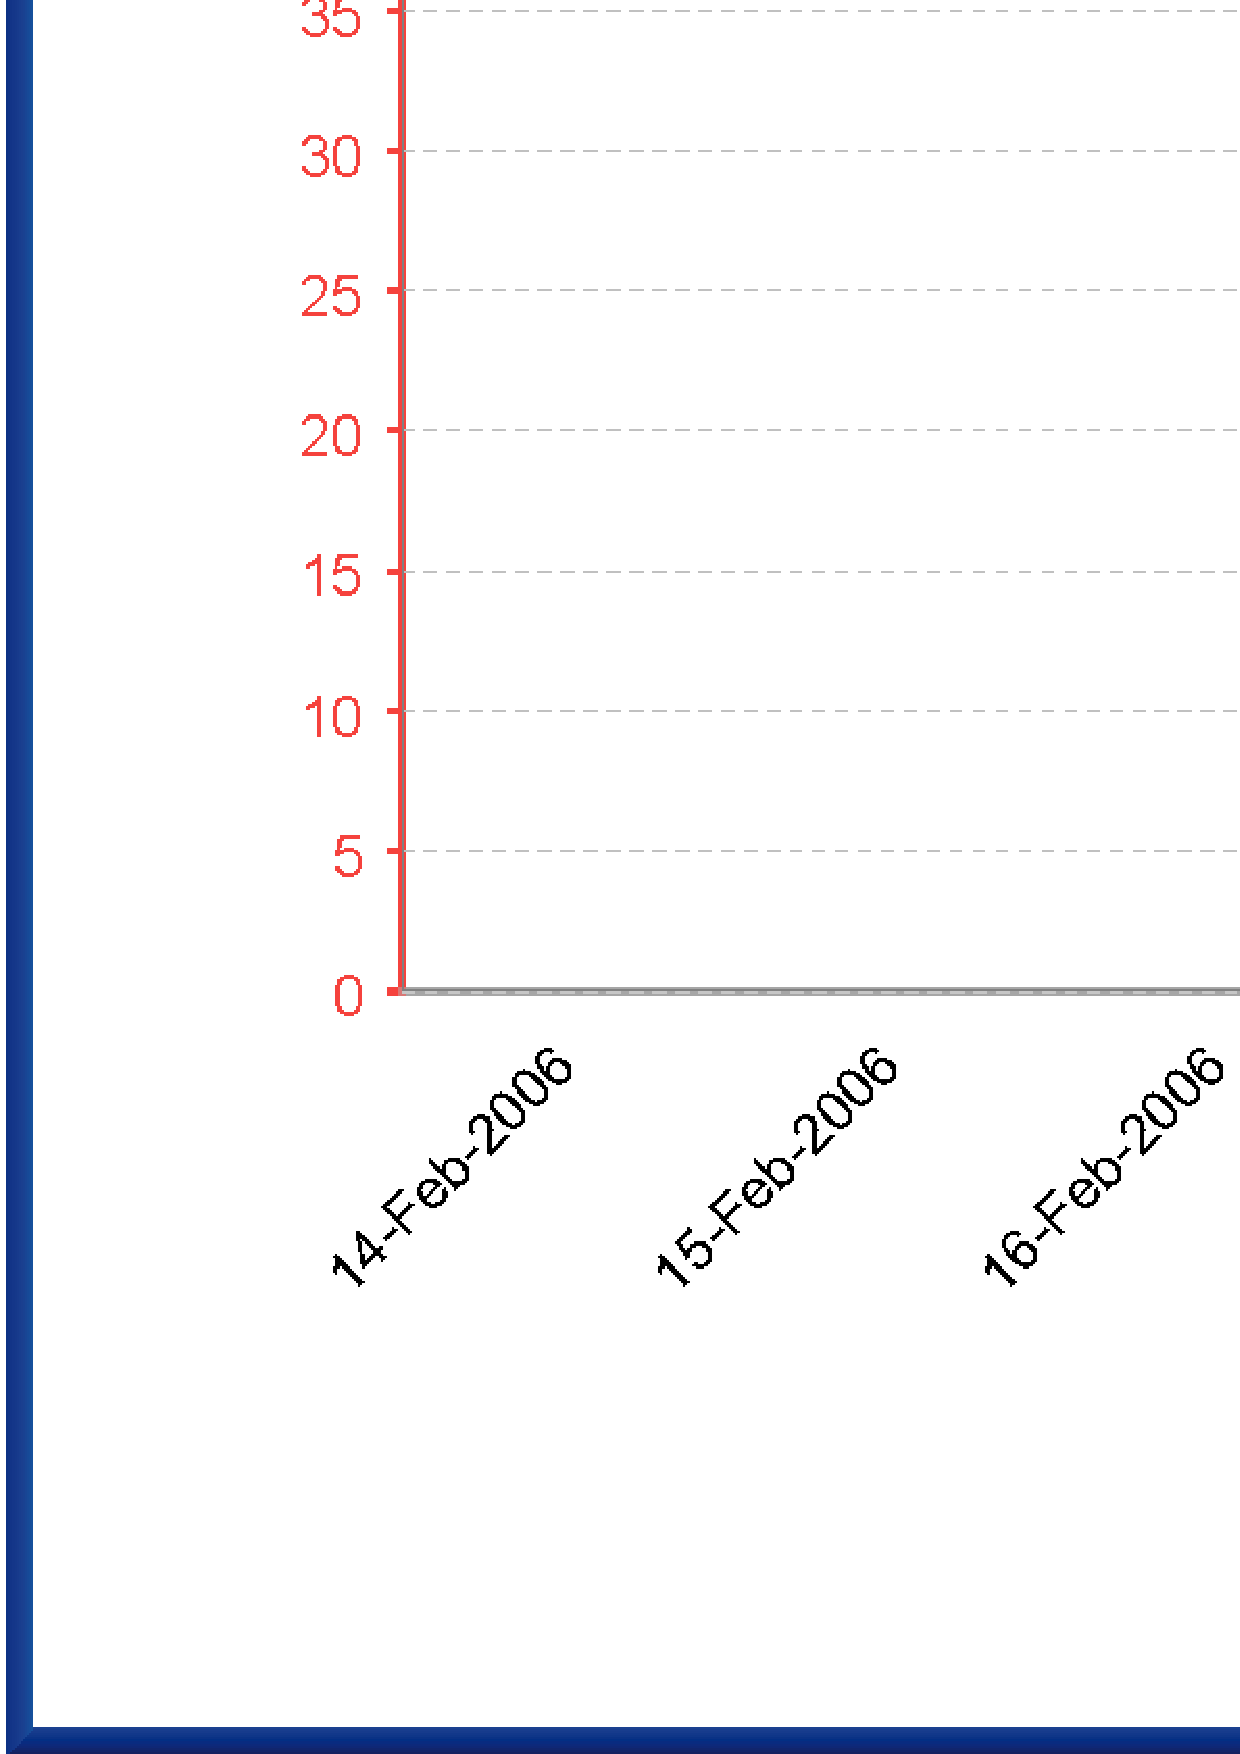
\includegraphics[width=0.70\textwidth]{figures/CSDL-CoverageSensorVerification}
  \caption{Telemetry Chart Indicating ``Emma'' Sensor not Working} 
  \label{fig:CSDL-CoverageSensorVerification}
\end{figure}

\begin{figure}[p]
  \center
  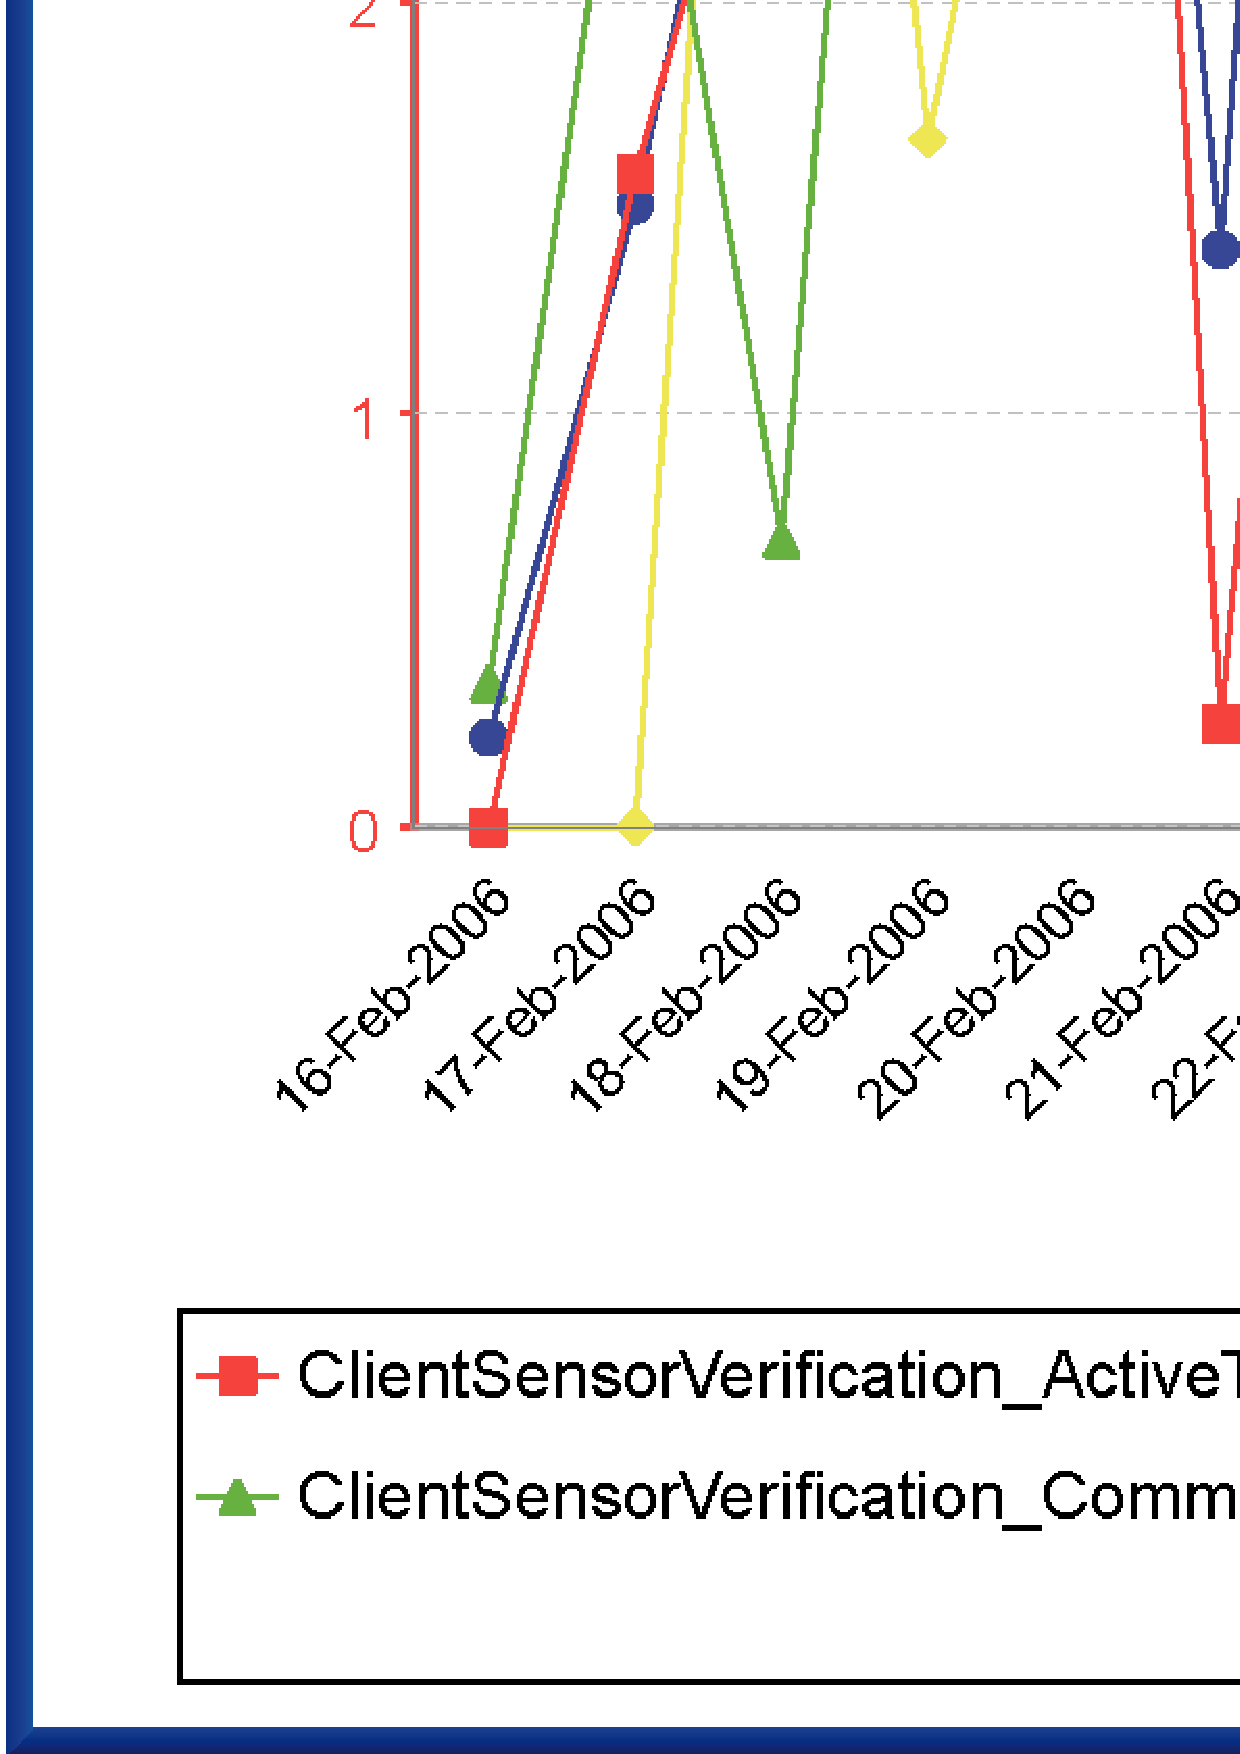
\includegraphics[width=0.70\textwidth]{figures/CSDL-DeveloperSensorVerification}
  \caption{Telemetry Chart Indicating ``Eclipse'' Sensor not Working} 
  \label{fig:CSDL-DeveloperSensorVerification}
\end{figure}











%%%%%%%%%%%%%%%
%  S T O R Y  %
%%%%%%%%%%%%%%%
\clearpage
%\subsection{Software project telemetry will not likely to provide value where low-level details are needed.} 
\subsection{Limitation on Low-level Details}
\label{EvaluationInCSDL:EventsDescription:Limitation}

\subsubsection{Pre-hypothesis Data:}
\begin{itemize}
  \setlength{\itemsep}{0pt}
  \setlength{\parskip}{0pt}
  \item 2006-02-05-1: I designed telemetry charts for the telemetry wall. Some of the charts were devoted to project level and individual level release cycle issue tracking. 
  \item 2006-02-06-1: I introduced the telemetry wall in the weekly status meeting. While the project level issue tracking charts were found \textit{``highly useful''} by the project manager, the individual level issue tracking charts were completely useless. One developer commented: \textit{``I would rather look into \textit{Jira} directly, because I don't know which issues remain.''} The project manager commented: \textit{``I would not be interested in those individual charts.''}
\end{itemize}

\subsubsection{Generated Hypothesis:}

The plausible explanation was related to information abstraction. Telemetry analyses offer high level perspectives on software development process by discarding low level details. The project manager's job was to make sure progress has been made and the software can be released as scheduled. He did not have to know low level details about individual issue. Project level issue tracking charts had the right level of abstraction to help him make release cycle decisions. On the other hand, the developers had to know issue details in order to fix them, but such information had already been discarded by telemetry analyses. 

\subsubsection{Intervention:}

None, except that I removed the individual level issue tracking charts from the telemetry wall.

\subsubsection{Post-hypothesis Data:}
\begin{itemize}
  \setlength{\itemsep}{0pt}
  \setlength{\parskip}{0pt}
  \item 2006-04-25-1: I modified the code issue telemetry chart to track the number of warnings falling into ``fail'' and ``monitor'' categories. The chart was primarily designed to be used by the project manager. I enhanced FindBugs report. Warnings in the ``fail'' category were highlighted in red color, and warnings in the ``monitor'' category were highlighted in blue color. I also modified the build script so that the developers could generate the report with single command on their workstations. This was primarily designed to be used by the developers to fix the warnings.
  \item 2006-05-06-1: Telemetry analysis indicated that all FindBugs warnings in the ``fail'' category had been eliminated. I had not received any complaint from the developers about the enhanced FindBugs report.
\end{itemize}

\subsubsection{Conclusion:}

The post-hypothesis data indicated that I had learned my lesson about information abstraction in telemetry analyses. Apart from the code issue tracking charts, I provided enhanced FindBugs report to supply low level details necessary for the developers to eliminate the potential bugs.
Both the issue tracking experience and the FindBugs experience seem to suggest that telemetry analyses will likely to provide decision-making value when a task requires relatively high level information abstraction, but they will not likely to provide value for tasks that require low level details.

\subsubsection{Elaboration:}

%This subsection reports on a failed attempt to use \textit{software project telemetry} to help an individual developer track \textit{``Jira''} issues assigned to him. 

At the early stage of this study, two of the scenes on the telemetry wall were related to release cycle issue tracking. One of them contained charts for project level issue tracking, while the other contained charts for individual level issue tracking. 
Figure \ref{fig:CSDL-Issue730} and \ref{fig:CSDL-Issue740} were two examples of project level issue tracking charts. The charts were a huge success with the project manager (see Section \ref{EvaluationInCSDL:EventsDescription:ProjectIssueTracking}), because they not only enabled him to track progress within each release cycle, but also established a baseline for future release cycle planning and scheduling.
The individual level issue tracking charts were similar to those for project level issue tracking. The only difference was that the individual issue tracking charts were developer-specific, and telemetry streams they contained represented the number of issues assigned to that specific developer instead of all the issues in the project. I provided each developer an individual issue tracking chart, intending to help him manage his assigned issues. However, the developers found the charts useless, and one of them commented: \textit{``I would rather look into Jira (the issue tracking database) directly, because I don't know which issues remain.''} The project manager found the charts useless too, and he commented: \textit{``I would not be interested in those individual charts.''}  

This was very interesting phenomenon. The project level issue tracking charts did not differ too much from the individual level charts. However, the former were found highly useful while the latter completely useless. 

My hypothesis was related to information abstraction. Telemetry analyses offer high level perspectives on software development. In other words, the analyses discard low level details. In case of release cycle issue tracking, the project manager's job is to make sure progress has been made and the software can be released as scheduled. He does not have to know about the details of each issue. The project level issue tracking charts offer the right level of abstraction to help him to make project management decisions. On the other hand, the developers' job is to resolve issues. They have to know the details about each issue, which means they have to delve into the issue tracking database to find the information. Besides, the CSDL developers usually have only 3 to 10 open issues to track at any moment. The abstraction in the individual issue tracking charts does not provide any value to them.

As a result, when I helped CSDL improve the utilization of ``CodeIssue'' metrics and FindBugs reports (see Section \ref{EvaluationInCSDL:EventsDescription:CodeIssue}), I learned from my previous experience. I used two sets of intervention procedures targeting the project manager and the developers separately. On the manager side, I provided a telemetry chart (see Figure \ref{fig:CSDL-FindBugs}) showing the number of FindBugs warning in \textit{``fail''} and \textit{``monitor''} categories respectively. The chart was monitored by the project manager as one of the project quality indicators. On the developers' side, I enhanced the original FindBugs report. Warnings in the \textit{``fail''} category were highlighted in red color, and warnings in the \textit{``monitor''} category were highlighted in blue color. For each reported potential bug, the enhanced report not only told the developers the category it belonged to, but also pinpointed the location in the source code from which it was generated.

The FindBugs experience appears to confirm the hypothesis. Both the issue tracking and the FindBugs experiences seem to suggest that telemetry analyses will likely to provide decision-making value when a task requires relatively high level information abstraction, such as project macro-management and high level process analysis. One the other hand, telemetry analyses will not likely to provide value for tasks that require low level details, such as resolving issues and fixing bugs.


\begin{figure}[tbp]
  \center
  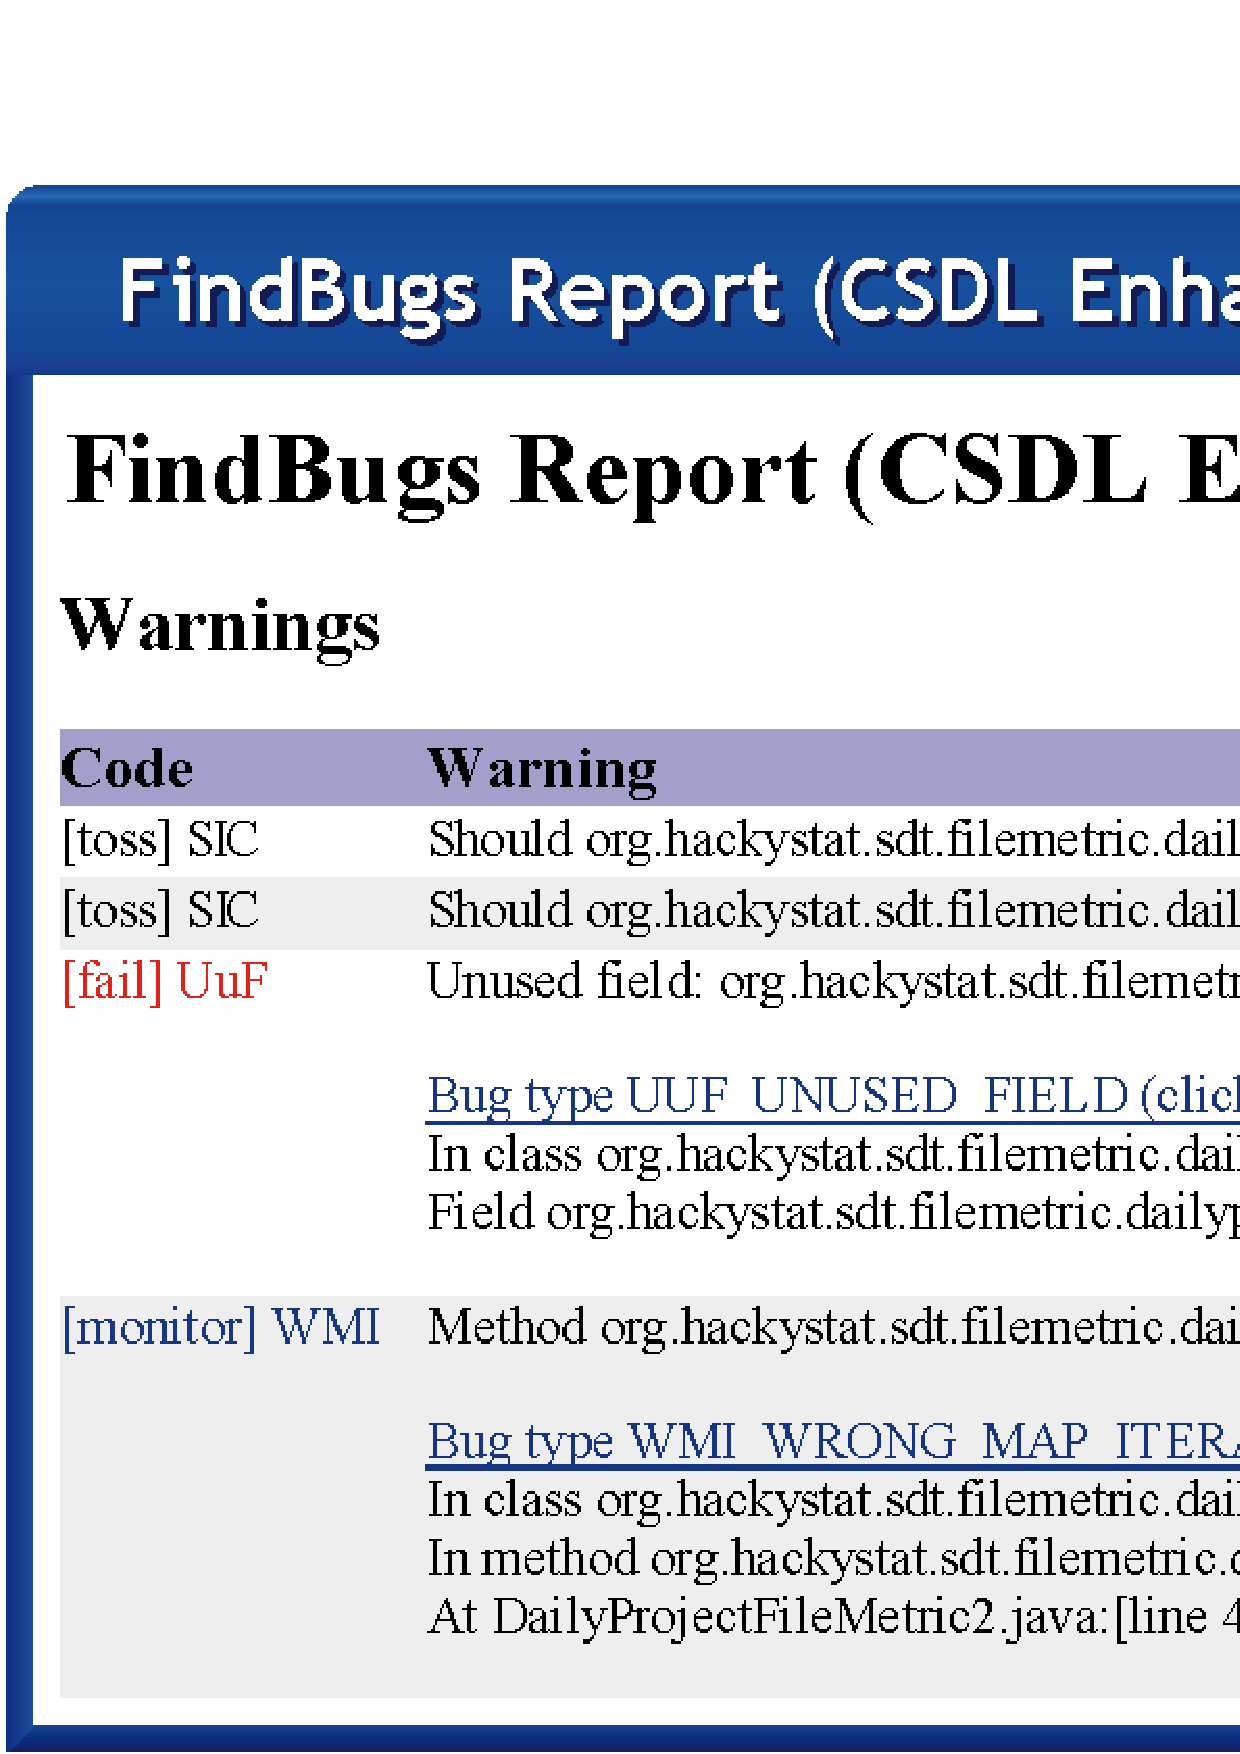
\includegraphics[width=1.00\textwidth]{figures/CSDL-FindBugsReport}
  \caption{CSDL Enhanced Version of FindBugs Report} 
  \label{fig:CSDL-FindBugsReport}
\end{figure}




%%%%%%%%%%%%%%%
%  S T O R Y  %
%%%%%%%%%%%%%%%
\clearpage
%\subsection{I enhanced the telemetry language with filter functions.} 
\subsection{Telemetry Language Enhancement with Filter Functions}
\label{EvaluationInCSDL:EventsDescription:FilterFunction}

\subsubsection{Pre-hypothesis Data:}
\begin{itemize}
  \setlength{\itemsep}{0pt}
  \setlength{\parskip}{0pt}
    \item 2006-02-20-1: While redesigning telemetry charts for the telemetry wall, I noticed several charts for module-level telemetry trends were overly cluttered (e.g., Figure \ref{fig:CSDL-UnfilteredCoverage}).
    \item 2006-02-21-2: I discussed the charts with three developers. They commented that those charts were too cluttered to be useful. One of them also noted that most of the lines were ``uninteresting'' because they represented inactive modules.
\end{itemize}

\subsubsection{Generated Hypothesis:}

The telemetry language could be enhanced with filter functions to filter out ``uninteresting'' telemetry streams. This could solve the usability and scalability problem with telemetry charts for large projects.  

\subsubsection{Intervention:}

I augmented the telemetry language to support nested function calls, and implemented special-purpose functions to support filtering telemetry streams in various ways.

\subsubsection{Post-hypothesis Data:}
\begin{itemize}
  \setlength{\itemsep}{0pt}
  \setlength{\parskip}{0pt}
  \item 2006-03-15-5: In an email request for comments, I brought up the idea of introducing nested function calls to the telemetry language.
  \item 2006-03-16-2: A Jira issue (HACK-612) was created to solve the usability and scalability problem of telemetry charts for large projects.
  \item 2006-03-17-2: The project manager used the telemetry wall to show the status of Hackystat development to outsider developers. For those overly-cluttered charts, he had to enlarge them to occupy all the nine screens to show the details.
%  \item 2006-03-17: I held a discussion with the project manager. We reached the consensus to implement filter functions as a special case of my recently proposed nested function calls.
  \item 2006-04-09-1: I finished the implementation of filter functions and closed the Jira issue (HACK-612).
  \item 2006-04-11-1: I revised the module-level coverage charts on the telemetry wall by applying filters to show only the top 5 and bottom 5 covered modules (e.g., Figure \ref{fig:CSDL-FilteredCoverage}). The developers liked the changes, but they requested a chart to show modules with coverage that changed most.
  \item 2006-04-17-4: I revised the filter function implantation, and made the chart showing modules with coverage that changed most available on the telemetry wall. One of the developers commented that filter functions made the chart not only much cleaner but also much useful. 
\end{itemize}

\subsubsection{Conclusion:}

The filter function is a useful enhancement to the telemetry language. It appeared to solve the usability and scalability problem with telemetry charts for large projects. 

\subsubsection{Elaboration:}

The initial telemetry language had only reduction functions, which take sensor data as input and output one or more telemetry streams. In the CSDL study, I noticed a significant usability and scalability challenge with telemetry charts to present ``interesting'' information from a large number of streams. For a large project, simple telemetry definitions could easily produce charts cluttered with dozens or even hundreds of lines. For example, Hackystat had over 70 modules, one frequent use of software project telemetry was to compare the values and trends of metrics between different modules. One of the charts on the telemetry wall used the following definition to present an overview of module-level test coverage in the Hackystat source: 

\begin{verbatim}
      y-axis yAxis(label) = {
        label, "integer", 0, 100
      };

      streams ModuleCoverageStreams() = {
        "Coverage by Modules",
        WorkspaceCoverage("Percentage", "**", "line")
      };

      chart ModuleCoverageChart() = {
        "Unit Test Coverage by Modules",
        (ModuleCoverageStreams(), yAxis("Percent"))
      };

      draw ModuleCoverageChart();
\end{verbatim}

It generated one telemetry stream for each individual module in the project. The resulting chart was shown in Figure \ref{fig:CSDL-UnfilteredCoverage}. It contained over 70 lines, which created a severe usability problem. Discussion with the developers revealed that they generally were only interested in a small subset of those lines, such as the modules with highest or lowest coverage or the modules with coverage that changed most. But it was overwhelming to locate such information in a chart cluttered with over 70 lines. 
%The developers wished there could be an automated mechanism to help them sift through the large amount of information. 

My hypothesis was that filter functions could be added to the telemetry language to filter out ``uninteresting'' telemetry streams, which could solve the usability and scalability problem with telemetry charts for large projects. Based on this hypothesis, I augmented the telemetry language to support nested function calls, and implemented special-purpose functions to support filtering telemetry streams in various ways.

The following example illustrated the use of two filter functions:

\begin{verbatim}
      streams ModuleCoverageStreams() = {
        "Coverage by Modules",
        Filter(
            FilterZero(
                WorkspaceCoverage("Percentage", "**", "line")
            ), "SimpleDelta", "Bottom", 3
        )
      };
\end{verbatim}

Both \textit{``Filter''} and \textit{``FilterZero''} were the name of filter functions. They were invoked on the stream expression for test coverage for all modules. In other words, the input to the filter functions was the output from the \textit{``WorkspaceCoverage''} reduction function, which was visually represented in Figure \ref{fig:CSDL-UnfilteredCoverage}. The \textit{``FilterZero''} function got rid of all lines with only zero values, while the \textit{``Filter''} function further reduced the set of telemetry lines to the three with the most significant decrease in value during the interval. The effect was to produce a chart showing the modules that were decreasing the most in test coverage. The resulting chart was illustrated in Figure \ref{fig:CSDL-FilteredCoverage}. It contained the modules potentially most in need of additional quality assurance resources.

\begin{figure}[p]
  \center
  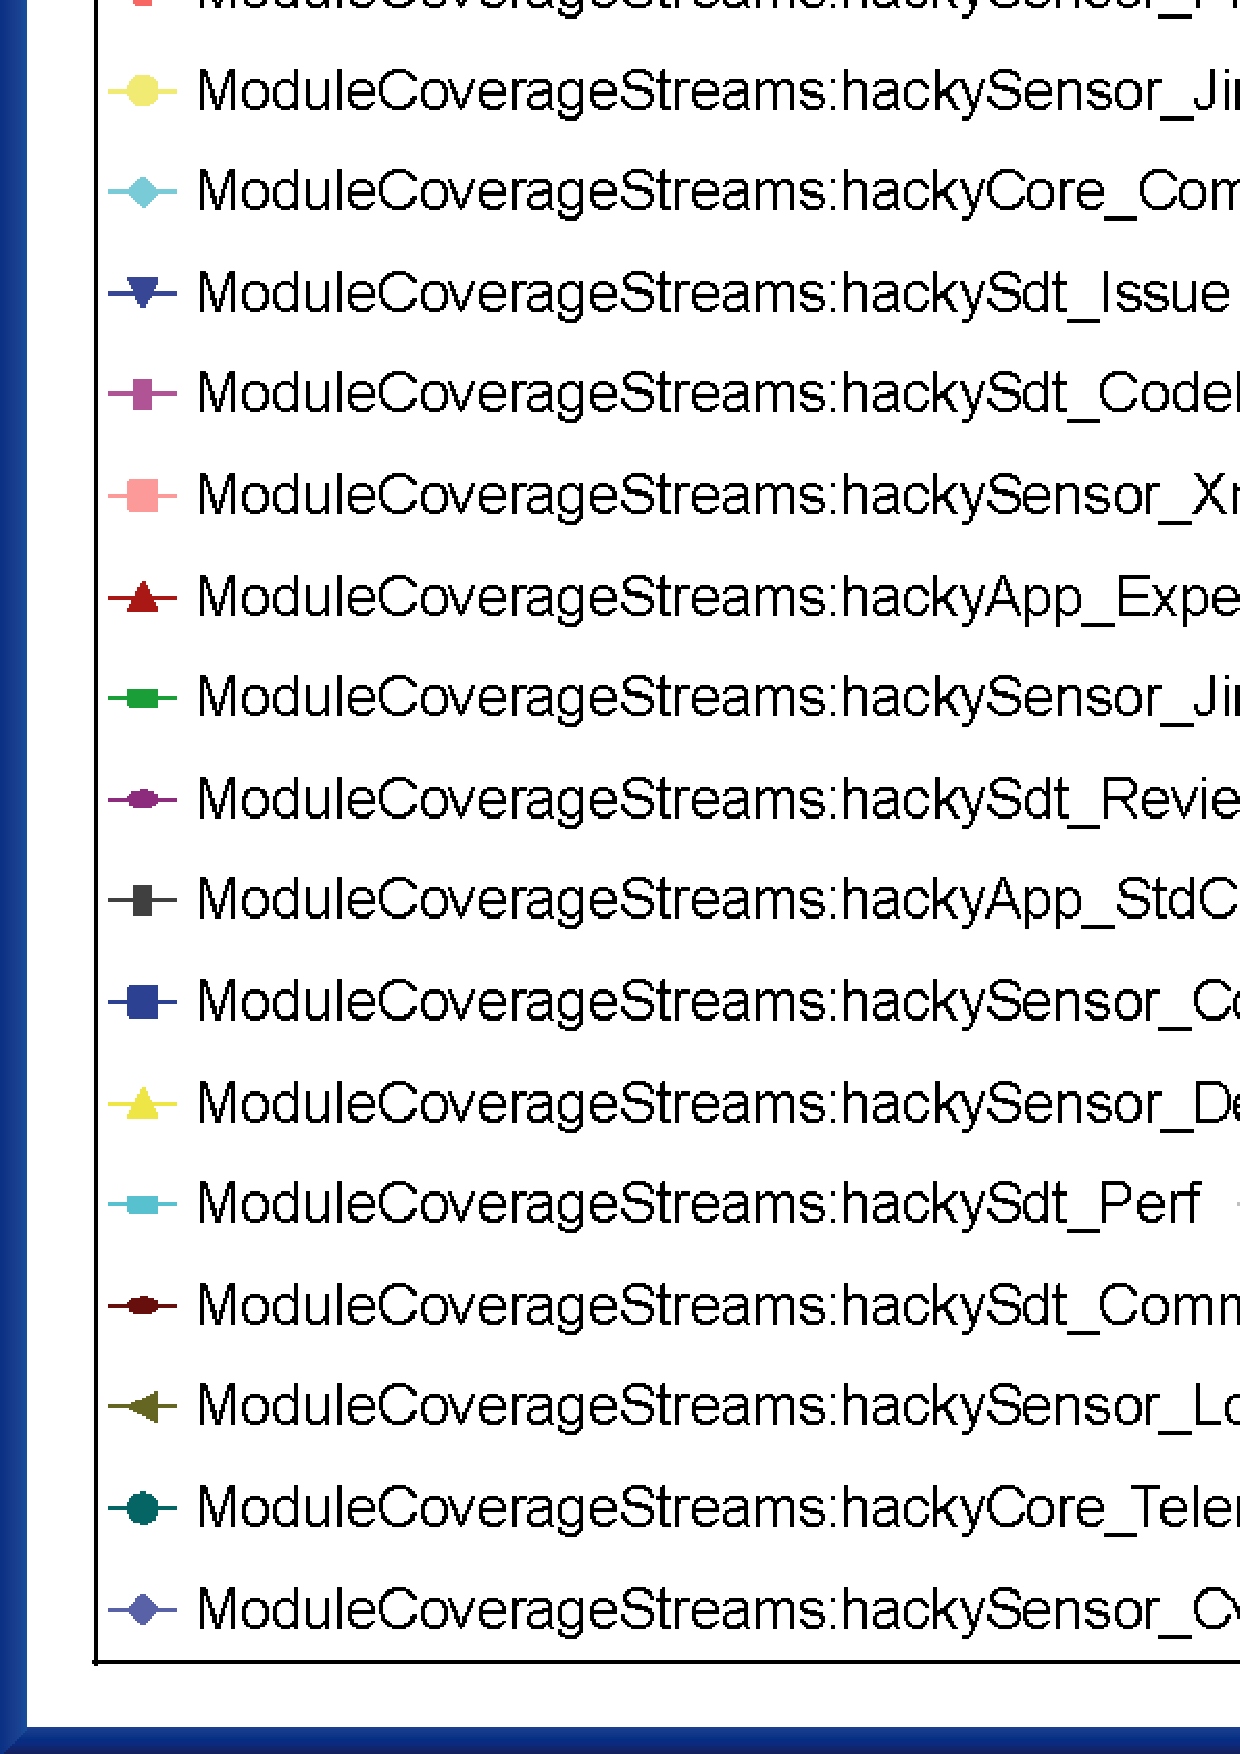
\includegraphics[height=0.93\textheight]{figures/CSDL-UnfilteredCoverage}
  \caption{Telemetry Chart with Unfiltered Module Coverage} 
  \label{fig:CSDL-UnfilteredCoverage}
\end{figure}

\begin{figure}[p]
  \center
  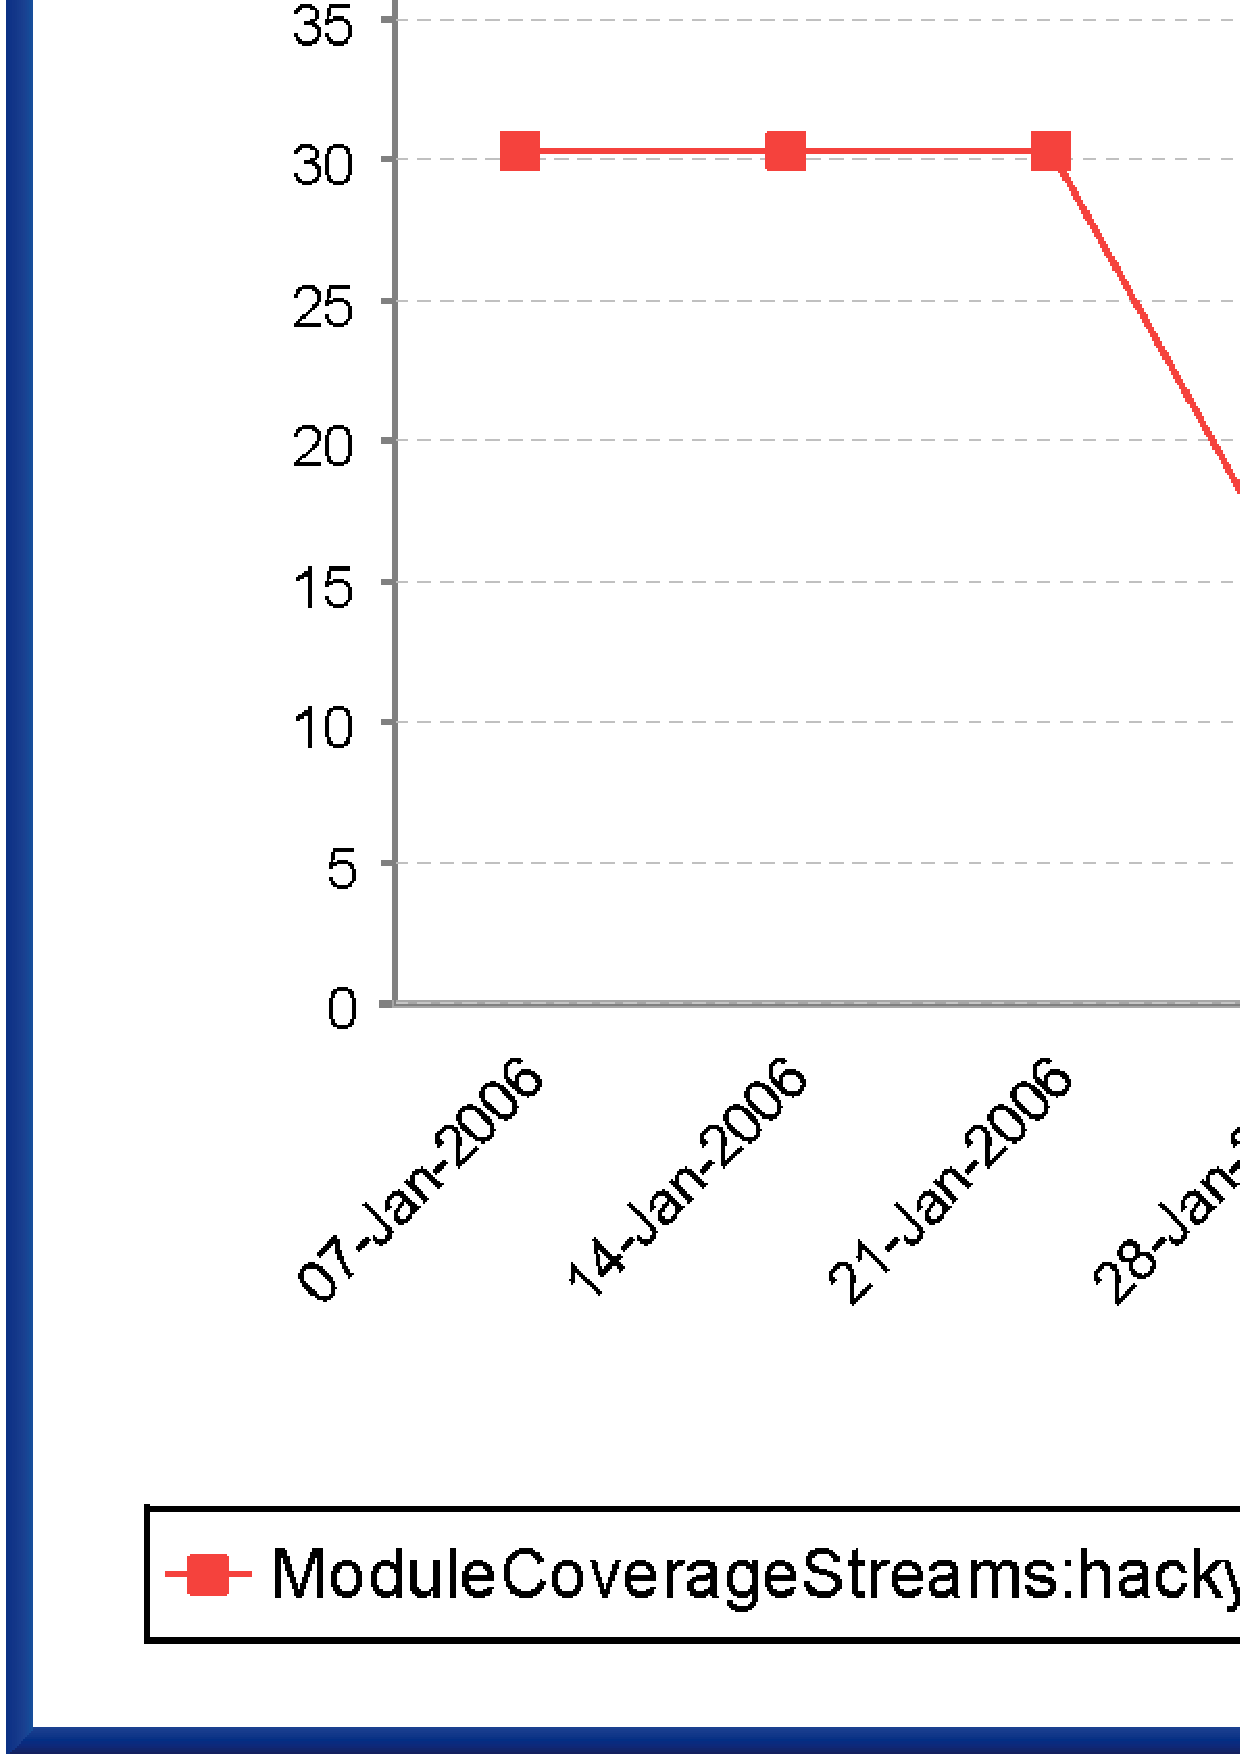
\includegraphics[width=0.70\textwidth]{figures/CSDL-FilteredCoverage}
  \caption{Telemetry Chart with Filtered Module Coverage} 
  \label{fig:CSDL-FilteredCoverage}
\end{figure}













%%%%%%%%%%%%%%%
%  S T O R Y  %
%%%%%%%%%%%%%%%
\clearpage
%\subsection{I enhanced the telemetry language with y-axis construct.} 
\subsection{Telemetry Language Enhancement with Y-axis Construct}
\label{EvaluationInCSDL:EventsDescription:VerticalAxis}

\subsubsection{Pre-hypothesis Data:}
\begin{itemize}
  \setlength{\itemsep}{0pt}
  \setlength{\parskip}{0pt}
  \item 2006-02-02-2: I showed some module level coverage charts to a developer. He noted that the automatically-scaled y-axis made comparison across related charts difficult.
  \item 2006-02-22-1: I discussed the module level quality indicator telemetry scene with the project manager. We had to check the vertical axis while comparing coverage trends in different modules.  
\end{itemize}

\subsubsection{Generated Hypothesis:}

It would be useful to allow a user to have the option to explicitly specify the range of the vertical axis in a telemetry chart. This way, related charts could be made more comparable by making them have the same vertical axis. The benefit of this extra level of control would outweigh the slight complexity it added to the telemetry language.

\subsubsection{Intervention:}

I augmented the telemetry language by adding \textit{``y-axis''} construct.

\subsubsection{Post-hypothesis Data:}
\begin{itemize}
  \setlength{\itemsep}{0pt}
  \setlength{\parskip}{0pt}
  \item 2006-03-16-1: During a discussion of telemetry charts with the project manager, I mentioned the idea of making relating charts more comparable by augmenting the telemetry language to allow a user to specify the vertical axis manually. He agreed that it would improve the usability of telemetry charts. 
  \item 2006-03-17-3: A Jira issue (HACK-616) was created to enhance the telemetry language to allow manually specified vertical axis.
  \item 2006-04-03-1: I held a discussion with the project manager, and we formalized the change to the telemetry language in order to allow a user to specify the vertical axis manually.
  \item 2006-04-09-2: I enhanced the telemetry language with \textit{``y-axis''} construct, and closed the Jira issue (HACK-616). 
  \item 2006-04-11-1: I update the telemetry wall, converting some charts to use manually-specified y-axises. I showed the changes to the project manager and the developers. They thought the change had improved the usability a lot, because comparisons could be made more intuitively with fixed vertical axises. 
\end{itemize}

\subsubsection{Conclusion:}

The user feedback after I enhanced the telemetry language with \textit{``y-axis''} construct suggested that it was a useful feature.

\subsubsection{Elaboration:}

%The telemetry wall is designed to display multiple telemetry charts simultaneously. The idea is to allow easy comparison of telemetry trends in related charts. For example, the developers might use the telemetry wall to compare test coverage in different modules. 

The telemetry language is designed to be as simple as possible. Most aspects of telemetry presentation are automated, so that a user does not have to fiddle with minute details such as fonts, colors, and layouts. The original language did not have a construct to allow a user to manually specify the range of the vertical axis in a telemetry chart. Instead, it was automatically determined based on the values of the telemetry data points. The result was a simpler language, but, at the same time, different charts might have different value ranges on their vertical axises. This approach worked well in most cases, especially when the range of telemetry data values could not be estimated in advance. However, in the CSDL study, I discovered that it also caused some inconvenience with some charts. For example, Figure \ref{fig:CSDL-AutoYAxis} was generated using definitions written in the original language:

\begin{verbatim}
      streams CoverageStreams(filePattern) = {
        "Coverage",
        JavaCoverage("Percentage", filePattern, "line")
      };

      chart CoverageChart(filePattern) = {
        "Unit Test Coverage",
        (CoverageStreams(filePattern))
      };
\end{verbatim}

The two charts showed test coverage for two different modules in the Hackystat source. By cursory examination, you might conclude that coverage in the two modules did not differ too much. However, if you paid attention to the vertical axises, your conclusion would be very different: the module \textit{``hackyApp\_Zorro''} had significantly higher coverage than \textit{``hackyApp\_PrjSize''}. Though the utility of the charts was not affected, it was a usability issue nevertheless, and the developers pointed out that the automatically-scaled vertical axises made comparison across charts difficult for such cases.

My hypothesis was that it would be useful to allow a user to have the option to explicitly specify the range of the vertical axis in a telemetry chart so that related charts could be made more comparable, and that the benefit of this extra level of control would outweigh the slight complexity it added to the telemetry language. As a result, I augmented the telemetry language with \textit{``y-axis''} construct, whose syntax takes the following form:

\begin{verbatim}
      y-axis <YAxisName> <ParameterList> = { 
          <Label>, <NumberType> (, <LowerBound>, <UpperBound>)?
      };
\end{verbatim}

\textit{`LowerBound`} and \textit{``UpperBound''} are optional fields. A user can choose to provide values to these optional fields to explicitly specify the vertical axis range. Otherwise, the range is determined automatically. With the new \textit{``y-axis''} construct, the telemetry definitions in the previous example have to be updated to a slightly complex form:

\begin{verbatim}
      y-axis yAxis(label) = {
        label, "integer", 0, 100
      };

      streams CoverageStreams(filePattern) = {
        "Coverage",
        JavaCoverage("Percentage", filePattern, "line")
      };

      chart CoverageChart(filePattern) = {
        "Unit Test Coverage",
        (CoverageStreams(filePattern), yAxis("Percent"))
      };
\end{verbatim}

The result was demonstrated in Figure \ref{fig:CSDL-FixedYAxis}, which showed the same coverage information for the same two Hackystat modules as in Figure \ref{fig:CSDL-AutoYAxis}. But this time the vertical axises in the two charts had the same range from 0 to 100. The difference in coverage for the two modules in Figure \ref{fig:CSDL-FixedYAxis} was obvious, and the comparison could be made more intuitively. The developers welcomed the changes.

\begin{figure}[p]
  \center
  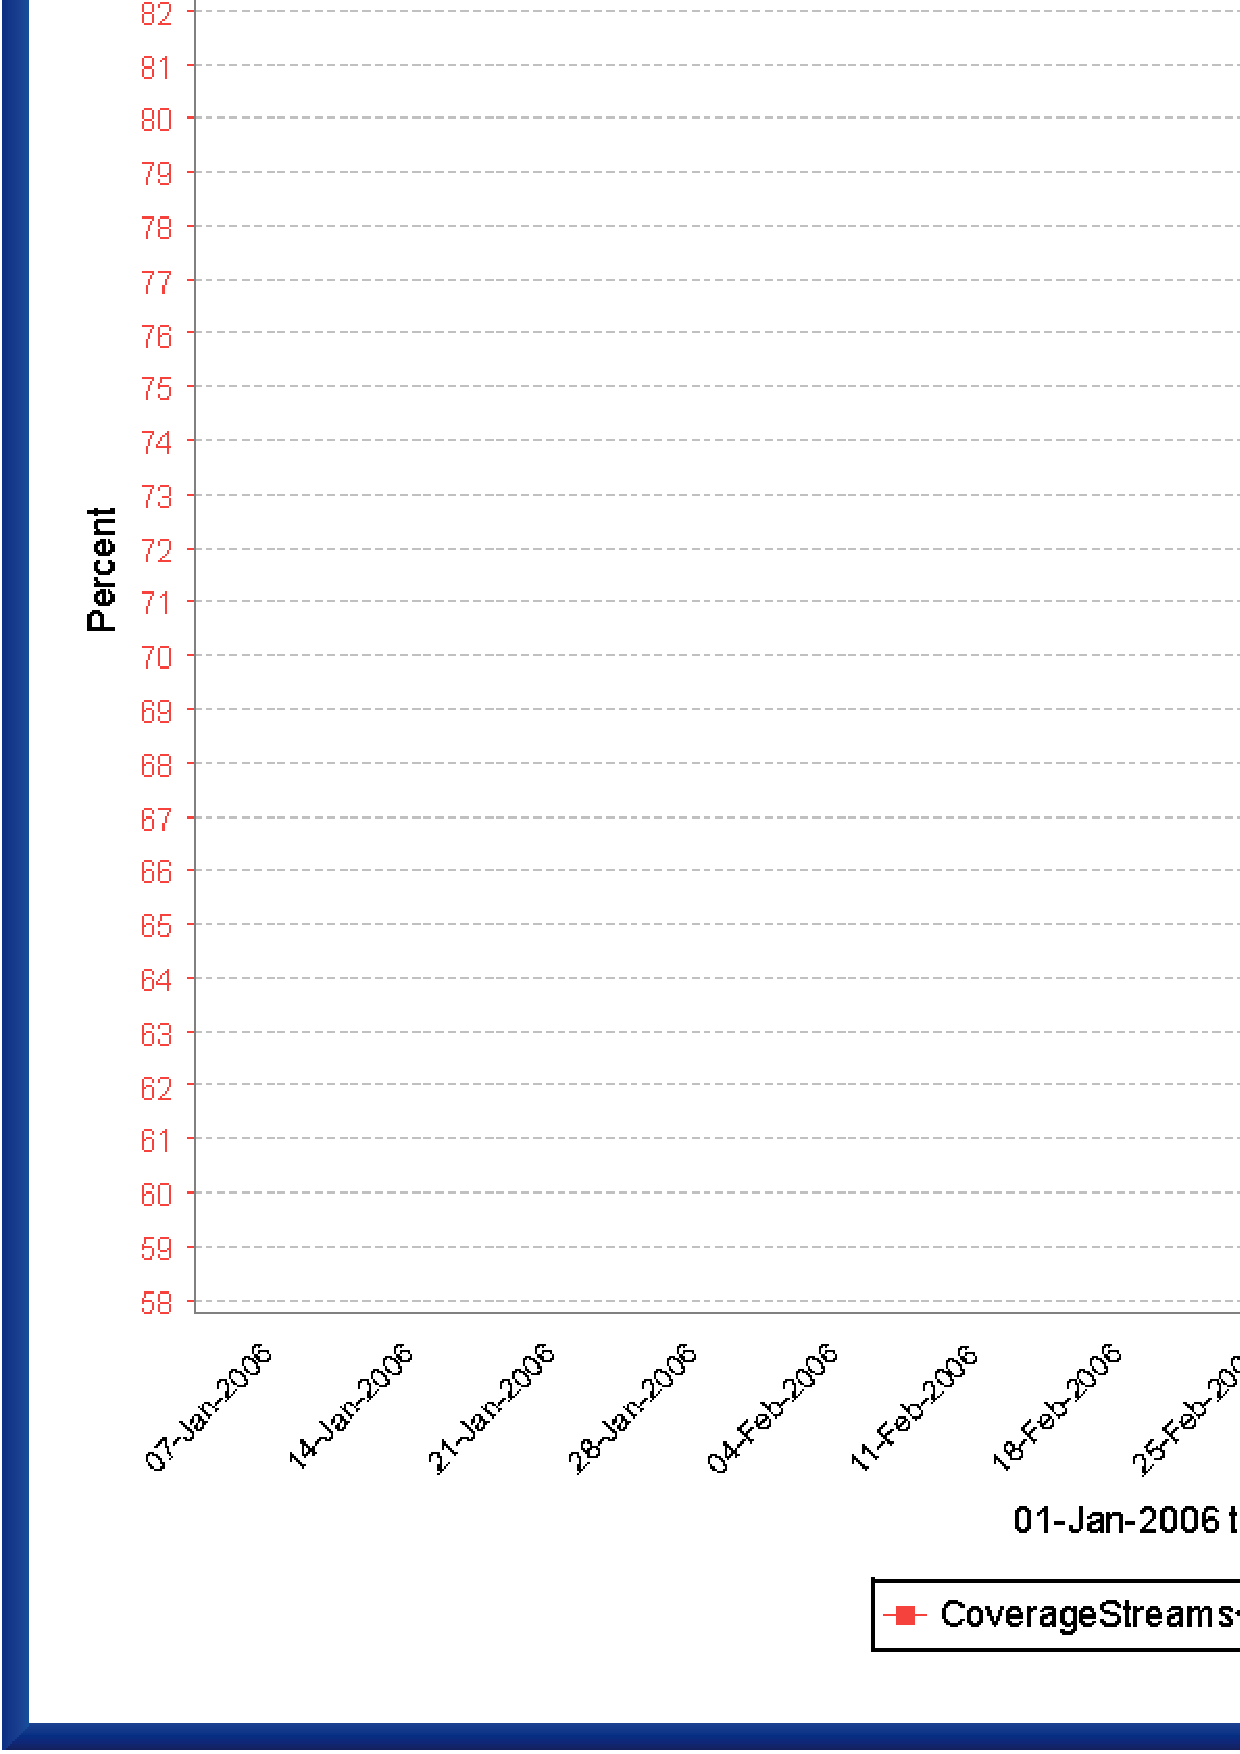
\includegraphics[width=1.00\textwidth]{figures/CSDL-AutoYAxis}
  \caption{Telemetry Charts with Automatically-scaled Vertical Axises} 
  \label{fig:CSDL-AutoYAxis}
\end{figure}

\begin{figure}[p]
  \center
  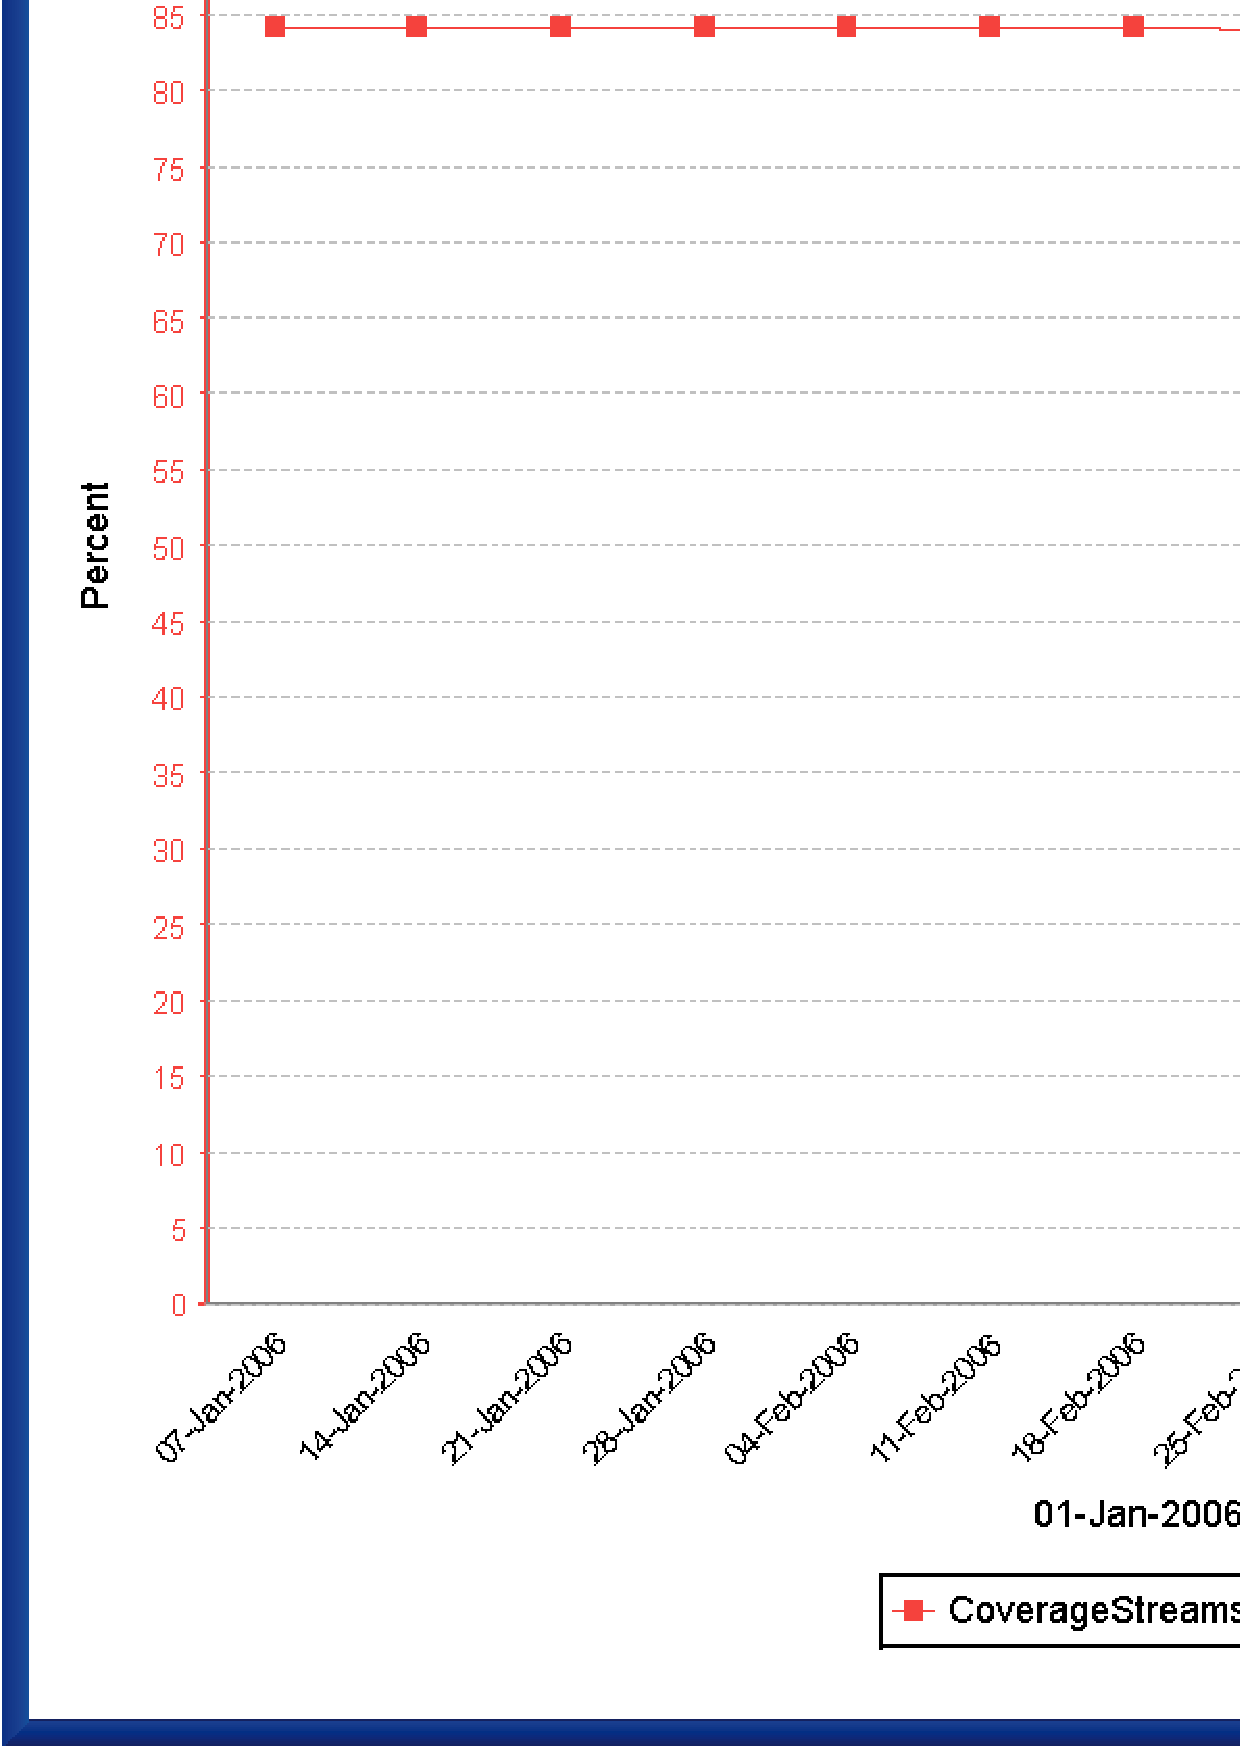
\includegraphics[width=1.00\textwidth]{figures/CSDL-FixedYAxis}
  \caption{Telemetry Charts with Manually-specified Vertical Axises} 
  \label{fig:CSDL-FixedYAxis}
\end{figure}



%%%%%%%%%%%%%%%
%  S T O R Y  %
%%%%%%%%%%%%%%%
%\subsection{G: It's Better to Hide the Telemetry Language from a Normal User.}








%%%%%%%%%%%%%%%
%  S T O R Y  %
%%%%%%%%%%%%%%%
\clearpage
%\subsection{I improved telemetry analysis runtime performance.}
\subsection{Runtime Performance Enhancement}
\label{EvaluationInCSDL:EventsDescription:Performance}

\subsubsection{Pre-hypothesis Data:}
\begin{itemize}
  \setlength{\itemsep}{0pt}
  \setlength{\parskip}{0pt}
  \item 2006-02-06-1: I demonstrated the telemetry wall in the weekly status meeting, and noticed that some of the charts covering long-term metrics trends could take several minutes to show up, which was more than the developers were willing to wait.
  \item 2006-02-13-2: I wanted to display some telemetry charts on the telemetry wall in the middle of the weekly status meeting, but encountered severe server timeout.
  \item 2006-02-23-1: One of the developers toggled the telemetry wall in auto-update mode. The server stopped responding under the heavy load, and its CPU usage stayed at 100\%. I had to restart the server.
\end{itemize}

\subsubsection{Generated Hypothesis:}

The performance problem was caused by the bottleneck in the data persistence layer, which used XML files to store sensor data. Given that machine processing of XML data was slow, the solution was to retain as many as possible the most often used sensor data instances in the cache.

\subsubsection{Intervention:}

I reviewed the code that interfered with the management of the sensor data cache, such as higher level user code not releasing references to sensor data instances. I modified the code to ensure that all references were released promptly.

\subsubsection{Post-hypothesis Data:}
\begin{itemize}
  \setlength{\itemsep}{0pt}
  \setlength{\parskip}{0pt}
  \item 2006-03-01-1: I reviewed the ``DailyProjectCoverage'' code, and found it that it never released references to sensor data instances, which was temporary data structure as far as ``DailyProjectCoverage'' is concerned. 
  \item 2006-03-05-2: The project manager created a Jira issue, requesting me to perform an audit on all daily project code to ensure references to temporary data structures were released.
  \item 2006-03-10-1: I started the code audit, and found several classes followed the same design pattern of ``DailyProjectCoverage,'' failing to release temporary data structures.
  \item 2006-03-11-2: After I sent out my findings, the project manager elaborated the distinction between ``cache'' and ``temporary data structure'' in an email to call to the attention of all the developers. 
  \item 2006-03-14-1: The server performance improved after the ``temporary data structures'' were properly disposed, but the improvement was not significant enough to reduce the telemetry wall response time to an acceptable range. I profiled the code with another developer, and we had a number of surprising findings. (1) When sensor data were cached in memory, over 90\% of processor time was spent on string comparison in workspace code. The case-sensitive comparison was 10 times more expensive than case-insensitive comparison. (2) The sensor data evolution mechanism in some classes was implemented very inefficiently. For example, the ``FileMetric'' class spent 80\% of processor time in the ``recognizeData()'' method, even if the data were already stored in the newest format. (3) The cost of reading sensor data from XML files was negligible.

  \item 2005-03-15-3: I sent out an email to the developer mailing list reporting the performance profiling result.

  \item 2006-03-15-4: After reporting the performance profile findings, I received an email from a former developer. He had experimented with a Berkeley XML DB back-end and found no performance improvement at all.

  \item 2006-03-21-2: An external user, who managed his own server, reported degrading telemetry analysis performance proportional to server up-time. He had not picked up the recent fixes, but the problem reported was consistent with the effect of not releasing temporary data structure. 
  \item 2006-04-05-2: There was a performance complaint on the daily project details analysis.
  \item 2006-04-06-2: In an email, one of the developers noted that there were many redundant computations in the daily project details analysis.
%  \item 2006-04-06: I responded that the code in daily project classes was only optimized for telemetry analysis. The daily project analysis reused that code, but it had completely different data access pattern than the telemetry analysis.
  \item 2006-04-07-2: One of the developers modified the ``DailyProjectUnitTest'' code taking advantage of its data access locality, and the result was remarkable: the analysis time for 2006-04-05 unit test metrics was reduced from 124 seconds to 6 seconds.
  \item 2006-04-10-1: I did the same thing with the ``DailyProjectFileMetric'' code, and reduced the analysis time for 2006-04-05 file metrics from 180 seconds to just 1 second.
  \item 2006-04-10-2: The project manager was happy with the results. He wanted to formally document the design pattern as a best practice in the Hackystat developer guide in the summer.
\end{itemize}

\subsubsection{Conclusion:}

The generated hypothesis was wrong. The performance problem was not caused by the XML data persistence layer. Instead, the main culprit was the excessive calls to the workspace comparison code.

\subsubsection{Elaboration:}

The metrics collected by the sensors contain very low level information. For example, a file size metric only captures the size information for one single file. However, telemetry analyses are performed at a much higher project level. They typically have to aggregate hundreds or thousands of metrics for a large project like Hackystat just to compute a telemetry data point representing one single day. Furthermore, analyses performed at the interval of weeks or months are usually produced by first computing a set of analysis at the daily grain size and then combining them together in some fashion to obtain the week or month value. Multiply that by the many different kinds of metrics on which telemetry analyses could be performed, and the fact that the telemetry wall sends multiple concurrent requests in order to display related charts simultaneously, the strain on the server resources could be easily overwhelming. 

At the beginning of this study, I found that the telemetry wall response was sluggish at best. It usually took more than several minutes for a telemetry scene to show up. I even experienced several incidents in which requests timed out and I had to restart the server to fix the problem. The sluggish performance caused a usability problem. You just cannot expect a user to push a button and then wait for several minutes for the result in an interactive situation.

Since software project telemetry was implemented as a Hackystat extension, the performance problem was intricately related to the Hackystat framework. The framework stores sensor data in XML files and uses extensive in-memory cache to improve system response time. My hypothesis for the performance problem was that it was caused by the bottleneck in the data persistence layer. Given that machine processing of XML data was slow, the solution was to retain as many as possible the most often used sensor data instances in the cache. Therefore, I started to look for code that interfered with the management of the sensor data cache, such as higher level user code not releasing references to sensor data instances. However, despite my effort of fixing the code, the performance improvement was not significant enough to reduce the telemetry wall response time to an acceptable range. I began to believe that there was no way to improve the performance except by adding more memory to the server.

The turning point was the day when I profiled the system with another developer. We had a number of surprising findings. We discovered that most processor time was spent on string comparison in workspace code. We also discovered inefficiencies introduced in the recent sensor data type enhancement. However, the most shocking discovery was that the persistence layer was not a bottleneck at all, because the profiler indicated that the time spent reading and parsing sensor data from XML files was negligible. Based on the findings, the code was reorganized to minimize the number of string comparison instead of XML file read. The result was dramatic. In the most significant case, the time computing 2006-04-05 file metrics for all modules in the \textit{Hackystat} project was reduced from 180 seconds to just one second. 

My hypothesis was wrong. It reflected the intuition on my part. Though it explained the observed fact in the pre-hypothesis data well, it was inconsistent with the post-hypothesis data. The performance problem was not caused by the XML data persistence layer at all. I learned an important lesson through this experience: application performance improvement should be always guided by profiling data instead of intuition.










%%%%%%%%%%%%%%%
%  S T O R Y  %
%%%%%%%%%%%%%%%
%\clearpage
%\subsection{An Experience of Empirically Resolving Some Metrics Contentions}
%\label{EvaluationInCSDL:Results:WhichMetrics}
%
%It's not uncommon in software metrics research and practice to see several definitions for a metrics. But, often time, there is not enough anecdotal evidence to support which definition of the metrics provides the best decision-making value. This subsection reports on my experience in CSDL to use \textit{software project telemetry} to empirically resolve such contentious problems for the \textit{Hackystat} project.
%
%For example, a former CSDL graduate student had developed a unit test coverage tool called \textit{``JBlanket''}\cite{Software:JBlanket}, which was subsequently adopted by the \textit{Hackystat} project. Since \textit{JBlanket} was only capable of computing \textit{method-level} coverage, the \textit{Hackystat} developers always wondered whether a more fine-grained criterion such as \textit{line-level} coverage would be a better indicator of code quality, and whether they should switch to a more-capable unit test coverage tool, such as Clover \cite{Software:Clover} and Emma \cite{Software:Emma}.
%
%The telemetry chart in Figure \ref{fig:CSDL-CoverageComparison} provides the empirical answer. It contains four telemetry streams about unit test coverage computed using four different criteria: \textit{class-level}, \textit{method-level}, \textit{block-level}, and \textit{line-level}. The chart indicates that though \textit{class-level} coverage might be too coarse-grained, there is no significant difference in the other three criteria except absolute values. As far as the \textit{Hackystat} project is concerned, the \textit{method-level} coverage provided by \textit{JBlank} has the same decision-making value as the more fine-grained \textit{line-level} coverage. Therefore, there is no need to replace \textit{JBlanket}.
%
%On a side note, CSDL did replaced \textit{JBlanket} with \textit{Emma} eventually. But the reason was a completely different one: \textit{JBlanket} was out of maintenance and incompatible with Java 5 byte code format.
%
%Another example was related to file size metrics. During the course of this study, CSDL developed an enhanced version of SCLC \cite{Software:SCLC}. It counts the size of 27 types of source code files, providing the number of comment, non-comment, blank, and total lines. CSDL used to use a size counting tool called LOCC \cite{Software:LOCC}. Compared to \textit{SCLC}, \textit{LOCC} only counts Java size, but it can count the number of methods and Java classes which \textit{SCLC} cannot. The \textit{Hackystat} developers wanted to replace \textit{LOCC} with \textit{SCLC}, but they were not sure whether the loss of capability to count the methods and Java classes would impair their metrics-based decision-making capability or not. \textcolor{red}{Philip Comment: Must be explicit about the observational data that exists to support this.}
%
%The telemetry chart in Figure \ref{fig:CSDL-SizeComparison} provides the empirical answer. It contains three telemetry streams about the \textit{Hackystat} project size: the number of Java classes, the number of methods, and the number of uncommented source lines. The chart indicates that there is no significant difference in the three counting rules except absolute values. Therefore, replacing \textit{LOCC} has no negative impact on CSDL metrics-based decision-making capability.
%
%\begin{figure}[p]
%  \center
%  \includegraphics[width=0.70\textwidth]{figures/CSDL-CoverageComparison}
%  \caption{Test Coverage Measured by Different Criteria} 
%  \label{fig:CSDL-CoverageComparison}
%\end{figure}
%
%\begin{figure}[p]
%  \center
%  \includegraphics[width=0.70\textwidth]{figures/CSDL-SizeComparison}
%  \caption{System Size Measured by Different Criteria} 
%  \label{fig:CSDL-SizeComparison}
%\end{figure}








%%%%%%%%%%%%%%%
%  S T O R Y  %
%%%%%%%%%%%%%%%
%\subsection{Unable to use some metrics, no decision-making value.}
%\label{EvaluationInCSDL:Results:UnableToUseSomeMetrics}

%This section reports two type of metrics that were collected in CSDL, but I 
%
%1. Performance metrics.
%
%The idea is quite simple: a telemetry for performance, if goes down, then we investigate.
%We were never able to use this metrics: (1) test case non-typical, (2) same machine, subject to variable, (3) Java, non-deterministic, if there is slow memory leak, short period of performance test not able to reveal it. (4) Too much technology stack: tomcat, jvm, os.  
%
%2. Java dependency.
%
%Idea: complexity of modules or package or class. If it exceed a threashold, then we can do something.
%not even know how to define complexity, at what level.
%related to maintainability. good in theoty. In reality, famililarity most important. Everyone think his own module is easiest to maintain. 
%
%Internal cohesion, external dependency: all relative concept. Not sure whether those metrics are validated or not.
%
%BUT we are still collecting the data: (1) ESTABLISH	a baseline, (2) might be useful in the future, like findbugs.








%%%%%%%%%%%%%%%
%  S T O R Y  %
%%%%%%%%%%%%%%%
%\subsection{De-emphasize active time}
%\label{EvaluationInCSDL:Results:DeemphasizeActiveTime}
%
%IDE-sensor collects internal buffer size change event, and active time are calculated based on those event.
%
%CSDL-developer: only find it interesting, don't really care.
%The manager: don't really care.
%Eclipse sensor: Though still collect active time, but more emphasis were on other micro-process related event.




    
    




%%%%%%%%%%%%%%%%%%%%%%%%%%%%%%%%%%%%%%%%%%%%%%%%%%%%%%%%%
%                                                       %
%                   S E C T I O N                       %
%                                                       %
%%%%%%%%%%%%%%%%%%%%%%%%%%%%%%%%%%%%%%%%%%%%%%%%%%%%%%%%%
\clearpage
\section{Study Conclusion}  \label{EvaluationInCSDL:StudyConclusion}

The result of this study was positive. It provided direct evidence that software project telemetry has decision-making values. It enabled me to gain a number of valuable insights with respect to the use of software project telemetry. Finally, I was able to improve the telemetry system based on user feedback. 



\subsection{Decision-Making Values}

This study provided direct evidence that software project telemetry has decision-making value to the project manager and the developers. 

Software project telemetry improved CSDL issue management practice by allowing the project manager to track progress in each release cycle. The historical charts for finished release cycles helped CSDL establish a baseline for future release scheduling and planning. They enabled the project manager to make effort estimation at the the beginning of a new release cycle based on the relationship between active time (or calendar days) and the number of resolved issues in previous releases. They also enabled in-process monitoring and control in the middle of a release cycle by comparing the shape of the telemetry from the current release with the shape of the telemetry from previous releases (see Section \ref{EvaluationInCSDL:EventsDescription:ProjectIssueTracking}). 

Software project telemetry improved CSDL code quality. By categorizing the warnings reported by 
\textit{FindBugs} into different severity groups: \textit{fail}, \textit{monitor}, and \textit{toss}, it overcame the false-positive issue inherent in the warnings, gave the developers a better sense of their code quality, and provided them with incentive to eliminate potential software bugs (see Section \ref{EvaluationInCSDL:EventsDescription:CodeIssue}).

Software project telemetry also provided the developers with insights into their development processes. By providing process feedback, software project telemetry seemed to make the developers more aware of the cost associated with integration build failures, which helped them make more optimal trade-off decisions between reducing local quality assurance cost and reducing integration build failure cost. Though the relationship between software development processes and integration build results were too complex to determine, experience from this study seemed to suggest that with the help of software project telemetry the developers could learn from their past experiences and get \textit{``smarter''} about their local quality assurance practices (see Section \ref{EvaluationInCSDL:EventsDescription:BuildAnalysis}).





%Software project telemetry resolved some contentious metrics questions among CSDL developers. By empirically showing the history of size and coverage metrics computed with different criteria, CSDL developers were convinced that they did not differ too much in their decision-making values, at least in the context of the Hackystat project.






\subsection{Insights}

This study enabled me to gain a number of valuable insights with respect to the use of software project telemetry.

Though bottom-up telemetry design based on the types of metrics is able to generate hundreds of telemetry charts without significant effort, the charts lack clear purposes and are generally of little value. You just cannot expect a user to go through hundreds of charts to find the ones that are useful to them. Top-down telemetry design based on user goals, which is similar to the methods in the Goal-Question-Metric paradigm, yields most useful telemetry charts (see Section \ref{EvaluationInCSDL:EventsDescription:TopDownDesign}).

In contrast to the principle behind top-down telemetry design, it is best to collect whatever metrics you can regardless whether you need them or not. The rationale is very simple. Software project telemetry uses sensors to collect metrics automatically and unobtrusively. Given the low cost of sensor-based metrics collection, it could only benefit an organization to collect the extra metrics. Even though you don't need a metric today, it can still be used to establish a baseline for comparison tomorrow. For example, \textit{``CodeIssue''} metrics were considered useless by most developers at the beginning of this study, but it was later used to improve CSDL code quality (see Section \ref{EvaluationInCSDL:EventsDescription:CodeIssue}).

It seems that sensor data problems are unavoidable. Most problems I encountered during this study were caused by failures to update corresponding configuration when there is a change in the project, such as adding a new module. The good news is that software project telemetry can be used for self-validation. By monitoring data point dropout or sudden value change in telemetry streams, or violation of correlation rules in related metrics, a project manager or a developer can make quick assessment whether there is underlying sensor data problem or not. Therefore, it is highly recommended for a development team to set up telemetry charts specially designed for the purpose of sensor data verification, and appoint a dedicated person to examine these charts for early detection of sensor problem (see Section \ref{EvaluationInCSDL:EventsDescription:DataVerification}).

This study also revealed a limitation with software project telemetry. Telemetry analyses are designed to offer high level perspectives on software development process by discarding low level details. The experiences with \textit{``Jira''} issue tracking and \textit{``FindBugs''} metrics seem to suggest that telemetry analyses will likely to provide decision-making value when a task requires relatively high level information abstraction, such as project macro-management and high level process analysis. One the other hand, telemetry analyses will not likely to provide value for tasks that require low level details, such as resolving issues and fixing bugs (see Section \ref{EvaluationInCSDL:EventsDescription:Limitation}).





\subsection{Telemetry System Improvement}

Finally, I received valuable feedback from the developers about telemetry chart presentation. Based on the feedback, I was able to enhanced the telemetry language to improve the usability of telemetry charts (see Section \ref{EvaluationInCSDL:EventsDescription:FilterFunction} and \ref{EvaluationInCSDL:EventsDescription:VerticalAxis}).
This study also helped me understand runtime performance characteristics of telemetry analysis for large projects like Hackystat. After optimizing my code, I was able to improve analysis response time several-fold (see Section \ref{EvaluationInCSDL:EventsDescription:Performance}).  
All these improvements contributes to a smoother user experience with software project telemetry. 






  \chapter{Case Study at Ikayzo} \label{Chapter:EvaluationInIkayzo}

This chapter outlines a case study of software project telemetry that will be performed at Ikayzo\footnote{http://www.ikayzo.org} with open-source project developers. Open-source project development environment is different from those in classroom or CSDL. The development is collaborated by geographically dispersed developers and project decisions are decentralized. It presents significant challenge for software project telemetry technology to be adopted.

This chapter begins with a description of Ikayzo in Section \ref{EvaluationInIkayzo:Setting}.
Section \ref{EvaluationInIkayzo:Design} outlines the design and strategies of this case study and offers rationale for the decisions.
Section \ref{EvaluationInIkayzo:DataAnalysis} introduces data collection and analysis procedures.
Section \ref{EvaluationInIkayzo:Role} describes researcher's role.
Section \ref{EvaluationInIkayzo:Threats} discusses the limitations and threats. 
The expected results are described in Section \ref{EvaluationInIkayzo:Results}. 
%and the time frame of this case study is given in Section \ref{EvaluationInIkayzo:TimeFrame}.



%%%%%%%%%%%%%%%%%%%%%%%%%%%%%%%%%%%%%%%%%%%%%%%%%%%%%%%%%
%                                                       %
%                   S E C T I O N                       %
%                                                       %
%%%%%%%%%%%%%%%%%%%%%%%%%%%%%%%%%%%%%%%%%%%%%%%%%%%%%%%%%
 
\section{Ikayzo Setting} \label{EvaluationInIkayzo:Setting}

Ikayzo provides open-source projects with free hosting service, which includes source code version control, issue tracking and management, automated metrics collection and analysis, and wiki discussion board. All projects have to go through a screening process before they are hosted. Beyond that, Ikayzo does not participate in or have influence on the decision-making process of the hosted projects.

The metrics collection and analysis support is provided through the software project telemetry system. Unlike the case in the two previous studies where the developers have to install sensors and invoke telemetry analysis themselves, the software project telemetry system is hidden at Ikayzo in order to completely eliminate metrics collection and analysis overhead from the developers. I installed the sensors and pre-configured several telemetry charts. A background daemon process runs the telemetry analyses and updates the charts automatically every night. Users access telemetry metrics analysis results through a link on the web portal for each project. Figure \ref{fig:IkayzoTelemetryReport} shows the exposed telemetry analysis page for one of the projects.

\begin{figure}[p]
  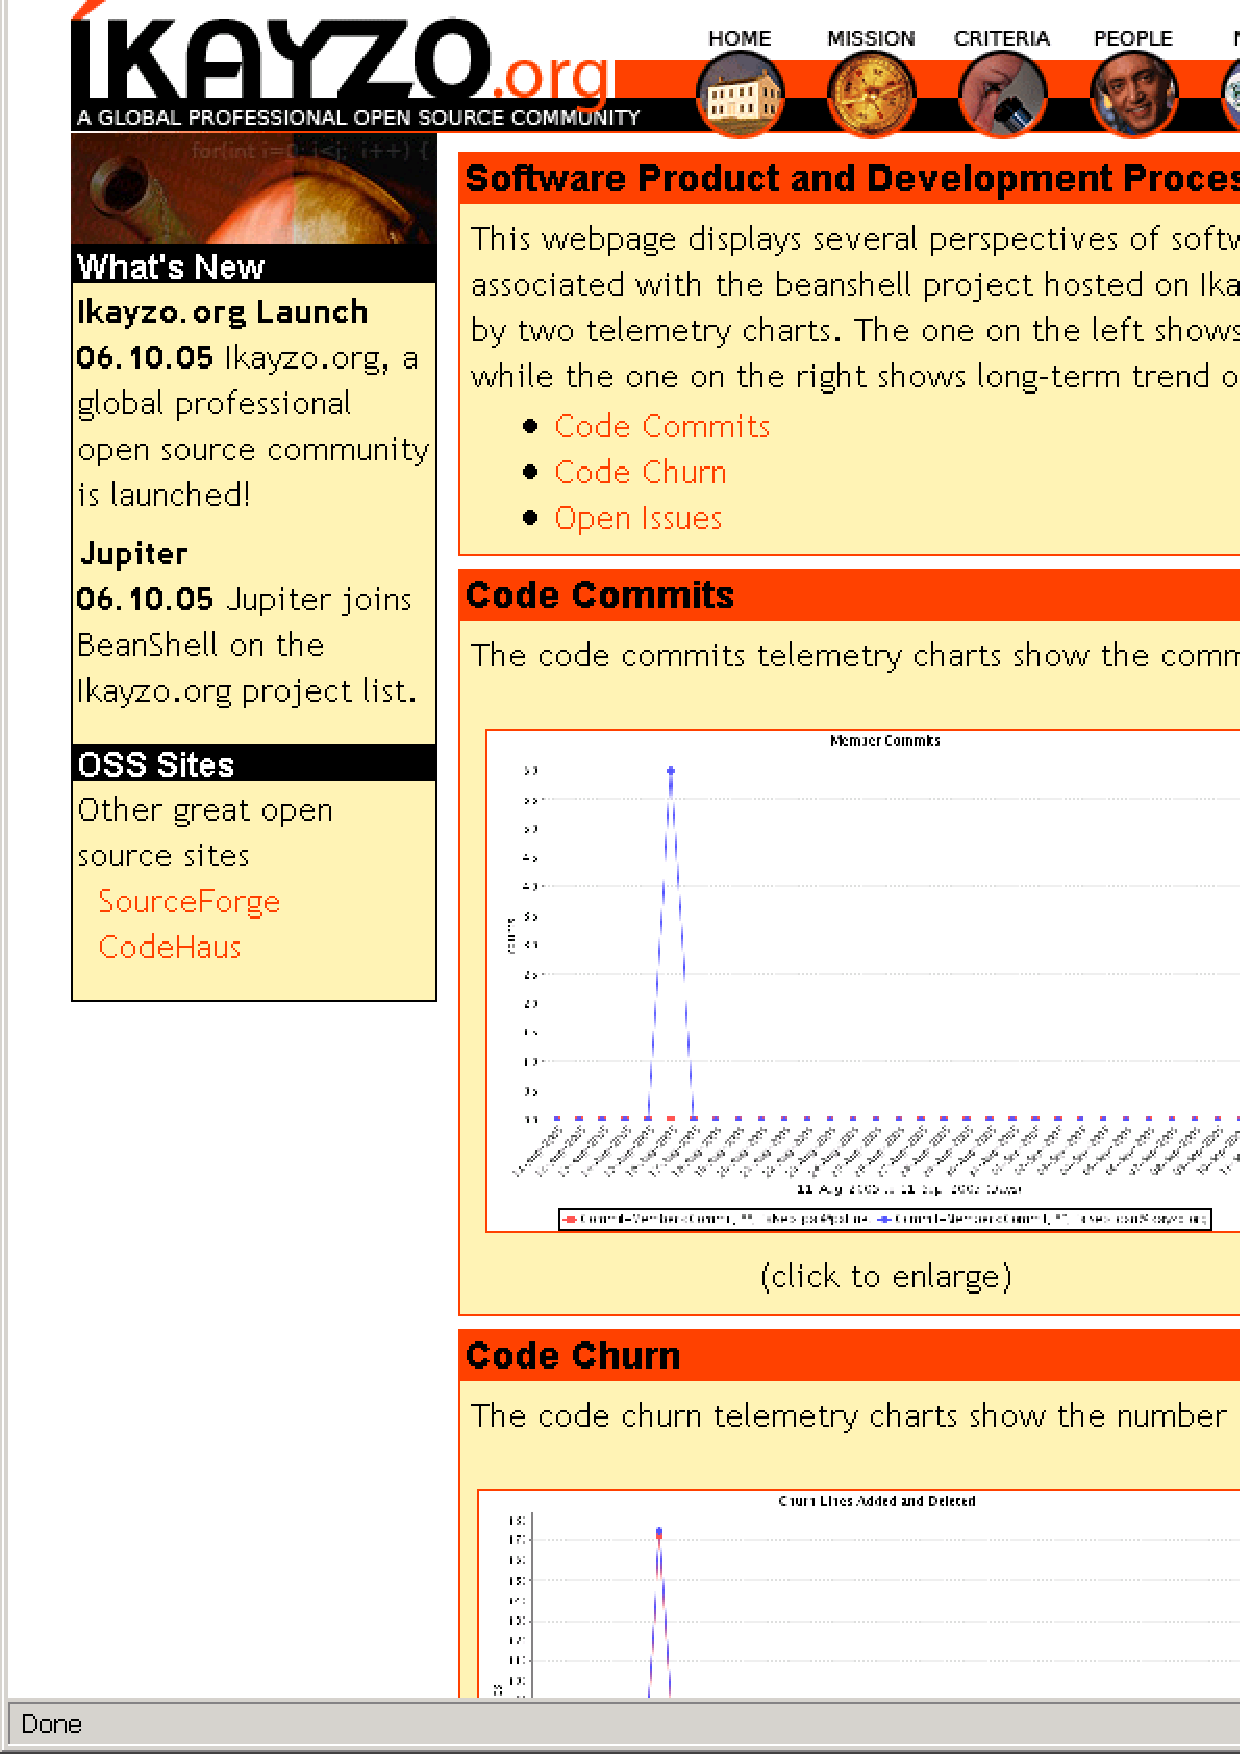
\includegraphics[width=1.00\textwidth]{figures/IkayzoTelemetryReports}
  \caption{Telemetry Reports for Ikayzo Hosted Project} 
  \label{fig:IkayzoTelemetryReport}
\end{figure}

Since the preliminary investigation by Ikayzo and me indicates that most developers are cautious about having their personal software process data being collected, such as which files they are editing at what time, we decided to only install server-side sensors. ``Server-side sensors'' refers to those sensors that monitor activities of various server systems, such as version control server, bug tracking and issue management server. Currently the following metrics are collected: (1) source code commit metrics, and (2) bug and issue metrics. We are planning to add source code size metrics in the near future. These metrics are all public knowledge because everybody can check out source code and browse project issue database through the web. What the software project telemetry system does is essentially make these aspects of the development process more transparent using telemetry charts.


The other services provide by Ikayzo are very much like those provided by other project hosting sites such as \textit{sourceforge.net} or \textit{java.net}, except that Ikayzo is much smaller in scale. As of this writing three projects are hosted by Ikayzo:

\begin{itemize}

	\item \textbf{BeanShell} is a small embeddable interpreter for a Java syntax compatible scripting language for the Java platform. The project has passed JSR-274 voting process, and is heading toward getting included in the Java Standard Edition at some point in the future.

	\item \textbf{Jupiter} is an Eclipse plug-in that provides code review and reporting functionality. It allows management of code annotations stored in XML based files, which can be shared by a development team.
	
	\item \textbf{SDL} stands for simple declarative language. It aims to provide an easy way to describe lists, maps, and trees of typed data in a compact, easy to read representation. Due to its simple API, it is a compelling alternative to XML for property files, configuration files, logs and simple serialization requires.	

\end{itemize}








%%%%%%%%%%%%%%%%%%%%%%%%%%%%%%%%%%%%%%%%%%%%%%%%%%%%%%%%%
%                                                       %
%                   S E C T I O N                       %
%                                                       %
%%%%%%%%%%%%%%%%%%%%%%%%%%%%%%%%%%%%%%%%%%%%%%%%%%%%%%%%%

\section{Case Study Design and Strategies} \label{EvaluationInIkayzo:Design}

Open-source software development environments differ from more traditional centralized software development environment in that development is performed through volunteer work, which makes it impossible to mandate what kind of technology should be used in development process. Both my previous experience and initial investigation at Ikayzo suggest that developers are cautious about their personal process data being collected. As a result, the approach employed at Ikayzo is to avoid those sensitive personal process data. The software project telemetry system is used only to collect and analyze metrics from publicly available source such as project source code repository and issue tracking system, and make these aspects of the development process more transparent by presenting them in a more useful telemetry format.

The goal of this case study is multiple:

\begin{itemize}
	\item To understand the adoption barrier of software project telemetry in an open-source environment where software development is collaborated through geologically-dispersed volunteer work and the decision-making process is decentralized. %All of which makes it infeasible to mandate the technology to be used. The experience with respect with the adoption barrier will not only help me to promote software project telemetry to an open source development environment, but other environment as well.
  \item To observe how software project telemetry is used in open-source development and find out what works and what does not work. 
	\item To understand both technical and social constraints of collection and analysis of different types of metrics in such an environment. 
%	\item To understand the administration cost associated with the current implementation of software project telemetry. 
\end{itemize}

%[Evaluation Strategy]
The evaluation in this case study will adopt the mixed methods paradigm. Since this will be largely a naturalistic study exploring how people use software project telemetry in an open-source development environment, priority will be given to qualitative information obtained during the course of this case study. 

The two most popular approaches in qualitative data collection are survey and ethnographic observation. Though ethnography has the advantage of enabling to observe how developers actually interact with software project telemetry and make project management and process improvement decisions, it is not chosen because of the fact that the open-source developers under this case study contribute to the projects through volunteer effort at their personal time from different locations. As a result, survey method is the only feasible choice to gather feedback. 

The decision to use survey method implies that I have to rely on the developers' self-reported opinions to evaluate software project telemetry. This threat can be mitigated by reconciling survey results with other data. Another source of data is quantitative information from telemetry report request log. If I find evidence that the developers look at telemetry report regularly, then I can put more confidence in their answers when they say software project telemetry is useful or not useful.




%Project metrics are another source of quantitative data, but I doubt they will be interesting since the projects are not that active.

%Software project telemetry system administration effort --- Since I am the person responsible for providing automated metrics collection and analysis support to projects hosted by Ikayzo, I am keeping a detailed diary of the effort I spend performing my task. I am the developer of software project telemetry reference implementation and various components in Hackystat framework, I am quite familiar with the system. My effort can be viewed as the lower bound of providing software project telemetry metrics support to an organization. I will reflect the difficulties I encountered, which are the potential adoption barriers of the technology.




%%%%%%%%%%%%%%%%%%%%%%%%%%%%%%%%%%%%%%%%%%%%%%%%%%%%%%%%%
%                                                       %
%                   S E C T I O N                       %
%                                                       %
%%%%%%%%%%%%%%%%%%%%%%%%%%%%%%%%%%%%%%%%%%%%%%%%%%%%%%%%%

\section{Data Collection and Analysis Procedures} \label{EvaluationInIkayzo:DataAnalysis}

This case study will collect data from two sources:
\begin{itemize}
	\item Qualitative data from surveys of the developer's opinion about software project telemetry. 
	\item Quantitative information about telemetry report requests.
\end{itemize}

The two sources of data will be integrated at data interpretation phase with emphasis on qualitative information and quantitative data corroborating the qualitative findings.





\subsection{Surveys}

Different approaches can be used to conduct a survey such as questionnaire or interview. In this case study, email questionnaires will be used for BeanShell project, and interviews will be used for Jupiter and SDL project. The reason is that the BeanShell project members are on the mainland and I don't have a chance to meet them in person, while I am able to meet other project members on a regular basis.

The survey, regardless of the approach chosen, will be conducted on a monthly basis. The purpose is to find out the developer's opinion about software project telemetry. The survey will follow the following basic steps:

\begin{itemize}
  \item Ask the developers how often they view telemetry reports. 
	\item Review telemetry reports together with the developers (omitted in email questionnaire).
	\item Find out what they think when they see the telemetry reports, and ask them whether the reports reflects the overall direction of the projects or not.
	\item Ask them what other telemetry analysis might be useful to them.
	\item Gradually introduce other available sensors and find out whether people are interested and under what condition they will use those sensors.
	\item Gradually reveal the regular telemetry analysis interface hidden underneath Ikayzo project portal which allow people to experiment with metrics themselves, and find out whether they exhibit interest beyond the predefined telemetry reports.
\end{itemize}





  
  

\subsection{Telemetry Report Requests}

Telemetry reports are integrated into the web portal for each project at Ikayzo. There are links on the main web page leading to telemetry charts. I will turn on web server logging facilities to log all telemetry chart requests. The information logged will include requester IP address, request time, and the telemetry chart being requested. The log will tell me the frequency of different telemetry charts being requested.

%This information can be correlated with project product metrics. We might find interesting correlations such as whether projects with constant development invoke telemetry analysis more often.;  (2) The popularity of different telemetry analysis.




%%%%%%%%%%%%%%%%%%%%%%%%%%%%%%%%%%%%%%%%%%%%%%%%%%%%%%%%%
%                                                       %
%                   S E C T I O N                       %
%                                                       %
%%%%%%%%%%%%%%%%%%%%%%%%%%%%%%%%%%%%%%%%%%%%%%%%%%%%%%%%%

\section{Researcher's Role} \label{EvaluationInIkayzo:Role}

Ikayzo uses software project telemetry system to provide automated metrics collection and analysis service to the projects hosted on its site. The system is designed and developed by me as part of my dissertation research. It is distributed under GPL license and everyone can use it free of charge. 

I provide volunteer technical support for Ikayzo running and administering its installation of software project telemetry system. My responsibility includes:
\begin{itemize}
	\item Setting up server-side telemetry sensors for automated metrics collection.
	\item Configuring software project telemetry system.
	\item Defining telemetry reports to present metrics analysis results.
	\item Writing scripts to update and publish telemetry reports automatically. 
	\item Monitoring the sensors and the system to make sure everything is working correctly.
\end{itemize}

My involvement in Ikayzo is strictly confined to providing software project telemetry system technical support. I don't provide support for other Ikayzo services, such as version control, bug tracking, and wiki discussion board. I don't participate in Ikayzo internal administrator. Finally, neither Ikayzo nor I have influence on the decision-making process of the hosted projects. 







%%%%%%%%%%%%%%%%%%%%%%%%%%%%%%%%%%%%%%%%%%%%%%%%%%%%%%%%%
%                                                       %
%                   S E C T I O N                       %
%                                                       %
%%%%%%%%%%%%%%%%%%%%%%%%%%%%%%%%%%%%%%%%%%%%%%%%%%%%%%%%%

\section{Threats, Verification, and Validation} \label{EvaluationInIkayzo:Threats}

\subsection{Measurement Validity}

Possible threat to measurement validity might come from qualitative data with respect to the developer's opinion of software project telemetry, but the risk is low. The reasons are as follows:

\begin{itemize}
	\item Neither Ikayzo nor I can influence the decision-making process and the overall direction of the hosted projects. The developers make volunteer contribution to project development. They don't get paid. There is no incentive for them to misrepresent their true opinions toward software project telemetry.
	
	\item Three open-source projects are involved in this case study. The developers' opinion from different projects will be compared and contrasted.
	
	\item All telemetry report requests are logged. The quantitative information will be used to corroborate the qualitative findings. 
\end{itemize}


\subsection{Internal Validity}

Internal validity refers to causality. In this case study, it is related to whether the telemetry reports have made the developers more aware of the status of the projects and thus contribute to better decision-making. Though this case study relies on the developers' subject opinion about the utility of software project telemetry, the threat is mitigated through the use of multiple data sources: data from 3 different projects, and quantitative and qualitative information from the the same project. All information will be reconciled and cross-validated at data analysis stage.


\subsection{External Validity}

External validity concerns the extent to which the experience gathered from the 3 projects hosted at Ikayzo can be generalized to other open-source development environment. 
The threat is quite low in this case study since the services provided by Ikayzo are pretty standard compared to other open-source project hosts such as \textit{sourceforge.net} or \textit{java.net}. 





%%%%%%%%%%%%%%%%%%%%%%%%%%%%%%%%%%%%%%%%%%%%%%%%%%%%%%%%%
%                                                       %
%                   S E C T I O N                       %
%                                                       %
%%%%%%%%%%%%%%%%%%%%%%%%%%%%%%%%%%%%%%%%%%%%%%%%%%%%%%%%%

\section{Expected Results} \label{EvaluationInIkayzo:Results}

Not all metrics can be collected in an open-source development environment. Some might be feasible to collect technically, but infeasible socially. The case study will allow me to better understand the constraints associated with metrics collection and analysis. The experience gathered in this case study will enhance my understanding of software project telemetry technology adoption barriers, not only in open-source development environments, but also in more closed traditional software development environments.





%%%%%%%%%%%%%%%%%%%%%%%%%%%%%%%%%%%%%%%%%%%%%%%%%%%%%%%%%
%                                                       %
%                   S E C T I O N                       %
%                                                       %
%%%%%%%%%%%%%%%%%%%%%%%%%%%%%%%%%%%%%%%%%%%%%%%%%%%%%%%%%

%\section{Time Frame} \label{EvaluationInIkayzo:TimeFrame}
%
%I expect to start the case study in October 2005. The study will last around four months.
%
%


% -what they want to see
% -what they think when they see the analysis
% -what they do after seeing the analysis.
  
  %\include{CaseStudyInClassroom} 
  %\include{CaseStudyInCSDL}
  %\include{CaseStudyInIndustry}
  %\begin{comment}

\chapter{Evaluation}  \label{Chapter:Evaluation}

Two techniques to use:
\begin{itemize}
	\item \textit{Questionnaires and Interviews:} quick and simple if one knows what to ask. However, inappropriate questions will lead to incorrect answer.
	\item \textit{Ethnographic Studies:} An external observation of the process. (Ref: Ian Sommerville, Software Engineering, sixth edition, Pearson Education, Essex, 2001.)
\end{itemize}

Telemetry analyses and their associated telemetry streams allow user to see the entire history of relevant software metrics and how they change from the beginning of the project. The project decisions are based not only on current values of metrics but also on their trend over time. Compared to the more traditional software management where decisions are mainly based on the current status of project, telemetry gives project managers and developers more information. The evaluation will investigate whether the extra information in telemetry-style management could result in early detection of problems and improvement of judgement or not.


The current Hackystat telemetry sub-system offer analyses in both expert mode and customized mode. In expert mode, user must use Hackystat telemetry language to instruct the system to build telemetry streams from collected metrics. Hackystat telemetry language is a custom language specifically designed for Hackystat telemetry sub-system. Though it is not difficult to learn, it still takes time for one to get comfortable with it. As a result, I developed customized-mode telemetry analysis, where Hackystat administrator or project owner can define telemetry streams before-hand using telemetry language, and users can run analysis by selecting any pre-define telemetry stream from a list. This saves ordinary user from learning a new language and lows adoption barrier at the cost of flexibility. There is a tradeoff to make. I will investigate which telemetry streams are frequently-invoked so that I can pre-define them and make them available in customized analysis by default. Custom-mode telemetry analysis invocation log can be analyzed to compute invocation count for each predefined telemetry stream or report. Expert-mode telemetry analysis invocation log can be used to find out new telemetry streams users are trying to generate. Based on above information, I can adjust pre-defined telemetry definitions.




Both quantitative and qualitative data will be collected. Quantitative data will include the actually usage of telemetry analyses on Hackystat server, and other software metrics related to evaluation subjects' software development processes. Qualitative data will be collected through surveys distributed in class, which will contain user feedback on telemetry-styled software project management and the usability of the current implementation of Hackystat telemetry sub-system.


Usage information can be collected automatically by instrumenting telemetry analysis on Hackystat public server. Before any user can access any service provided by the public server, Hackystat requires user to register an account. Each time an analysis is invoked, user information will be sent to the server along with other request parameters. Therefore, it's possible to collect information such as the content of the telemetry analysis being requested and the frequency the analysis are invoked by a particular user. Evaluation subjects' software development product and process metrics are the data collected by various Hackystat sensors.


Telemetry analyses are based on software projects registered with Hackystat server. When they are invoked, the project information will be available to instrumentation as well. This means that the project status (e.g. indicators of size, quality, effort, complexity, etc.) at the time telemetry analyses are invoked can be computed, which enables me to establish a statistical correlation between them. One possible conclusion from such exercise could be when software developers are spending lots of time on testing, they tend to invoke quality related telemetry analyses more frequently, and project coverage tends to go up. Note that this observation does not imply any causal relationship, it merely suggests that some events tend to happen together. But causal relationship might be established when user feedback is considered. 

\end{comment}
  
  \chapter{Conclusion}  \label{Chapter:Conclusion}


This research introduced \textit{software project telemetry}, which is a novel, light-weight measurement approach. It includes both (1) highly automated measurement machinery for metrics collection and analysis, and (2) a methodology for in-process, empirically-guided software development process problem detection and diagnosis. In this approach, sensors collect software metrics automatically and unobtrusively. Metrics are abstracted in real time to telemetry streams, charts, and reports, which represent high-level perspectives on software development. Telemetry trends are the basis for decision-making in project management and process improvement. It overcomes many of the difficulties in existing approaches.



\section{Anticipated Contributions}

The anticipated contributions of this research are:

\begin{itemize}
	\item The concept of software project telemetry as an effective automated approach to in-process, empirically-guided software development process problem detection and diagnosis. 
  
  \item An implementation of software project telemetry which allows continuous monitoring of software project status, as well as generating and validating software process improvement hypothesis.
  
  \item The insights gained from the case studies regarding how to use software project telemetry effectively for project management and process improvement, as well as the adoption barrier of the technology.

\end{itemize}





\section{Future Directions}

There are several areas I am unable to address within the time frame of this dissertation research. They will be future directions:

\begin{itemize}
  \item \textit{Telemetry analysis user interface improvement} --- Preliminary evaluation results suggest that the usability improvement to the interface invoking telemetry analysis is desired, especially with respect to the way telemetry analysis parameter values are supplied.
  
	\item \textit{Telemetry language measurement scale type checking} --- Current telemetry language does not enforce measurement scale type checking, and meaningless mathematical operations can be applied to telemetry streams as a result. The actual usage of the telemetry language needs to be studied to determine whether it is a big problem to end users or not. If it is, then the language needs to be augmented to account for scale type difference.
	
	\item \textit{Statistic process control} --- Given a set of telemetry streams, human judgment is required to detect bad trends in the development process. Statistic process control might provide automated support and needs to be studied in the context of software project telemetry.
	
	\item \textit{Replication of case study} --- The case studies need to be replicated in different settings in order to address external validity issues.
	
	\item \textit{User base expansion} --- One of the advantage of software project telemetry is that system deployment requires very little resource. This means the technology adoption risk is quite low for a software organization. I will make user interface improvements and try to find opportunities to market the technology.
\end{itemize}














%\section{Research Summary}
%\section{Research Contributions}
%\section{Lessons Learned}
%\section{Future Directions}


%%%%%%%%%%%%%%%%%%%%%%%%%%%%%%%%%%%%%%%%%%%%%%%%%%%%%%%%%%%%%
%%
%%   Comment Start
%%
%%%%%%%%%%%%%%%%%%%%%%%%%%%%%%%%%%%%%%%%%%%%%%%%%%%%%%%%%%%%%
\begin{comment}


\section{Lessons Learned}


\subsection{Automated data collection is necessary}

Two advantages: (1) Lower data collection overhead, reduce metrics program adoption barrier. (2) Increase data accuracy. (3) Data collection in daily integration build system is important.



\subsection{Perfect solution may not be feasible}

Trying get perfect metrics may not be possible. A good example of this problem is our solution for unit test coverage computation. There are several definition of coverage:
\begin{itemize}
	\item branch level
	\item statement level
	\item method level
\end{itemize}

All have their advantages and disadvantages. Branch level coverage information indicates whether all excution path of the program has been exercised or not. It is the most accurate measure, but hard to collect at the same time.

Method level without one line method.



\section{Future Work}

\subsection{Etiquette of Data Elements}

Experience has proved numerous times that appropriate using of data is one of the most important elements to get any metrics program off the ground. If individuals see the metrics as tools to help them improve their software development processes, they are more likely to embrace the program. However, on the other hand, if they feel metrics program is used by the management to monitor their behavior, they are likely to resist it or even fake data.


Software measurement activities will be subverted if they are seen as a threat, ignored if thought incompetent or inappropriate, or discredited if they do not deliver the anticipated benefits.

There are two important issues that must be addressed:
\begin{itemize}
	\item Data privacy issue. 
	\item Provide regular feedback to developers.
\end{itemize}	
	

There should be specific rules regarding who can access what portion of data, and when data go from private to public. Some data should always be kept private to individual developers, while other data can be accessed at the project or organizational level. In particular, metrics should never be allowed to measure individual performance. Robert Grady [Grady 92] has suggested the following recommendations:

\begin{table}[tbp]
  \centering
    \begin{tabular}{|p{4.5cm}|p{4.5cm}|p{4.5cm}|} 
      \hline
      Individual & Project Team & Organization \\
      \hline
      %% row 2 column 1
      Defect rates (by individual)\newline Defect rates (by module)\newline 
      Defect rates (under development)\newline Number of compiles &
      %% row 2 column 2
      Defect rates (team)\newline Module size\newline Estimated module size\newline 
      Number of re-inspections\newline Defects per module (prerelease) &
      %% row 2 column 3
      Defect rates (by project)\newline Size (by product)\newline Effort (by project)\newline 
      Calendar times\newline Defects per module (post release)\newline 
      Effort per defect (average) \\ 
      \hline
    \end{tabular}
  \caption{Data Access Recommendations}
  \label{tab:DataAccessRecommendations}
\end{table}



\subsection{Privacy Issue}
The access rules need to be enforce at the tool level. What is Hackystat conformance level???
	 
	 
	
	
\subsection{Top down approach, or knowledge repository}

In other words, the telemetry framework is practically useless if one cannot construct suitable telemetry streams to solve problems at hand. Therefore, a methodology for a goal-driven, top-down approach to design and validate telemetry streams is necessary to supplement the implementation and make the concept of telemetry-based software project management operable.

After validation, useful streams can be put into knowledge repository. But still, it might be context sensitive (similar to software process models).
	 
	
\end{comment}
%%%%%%%%%%%%%%%%%%%%%%%%%%%%%%%%%%%%%%%%%%%%%%%%%%%%%%%%%%%%%
%%
%%   Comment Start
%%
%%%%%%%%%%%%%%%%%%%%%%%%%%%%%%%%%%%%%%%%%%%%%%%%%%%%%%%%%%%%%

  
  \appendix
  \chapter{Software Project Telemetry Language Specification\\(Version 1.2)}  
\label{Chapter:TelemetryLanguageSpecification}



This document describes the syntax, semantics, and design of Software Project Telemetry Language. The language is neutral, and independent of any particular implementation.


 
%%%%%%%%%%%%%%%%%%%%%%%%%%%%%%%%%%%%%%%%%%%%%%%%%%%%%%%%%
%                                                       %
%                   S E C T I O N                       %
%                                                       %
%%%%%%%%%%%%%%%%%%%%%%%%%%%%%%%%%%%%%%%%%%%%%%%%%%%%%%%%%
\section{Introduction}  \label{TelemetryLanguageSpecification:Introduction}

Software Project Telemetry Language is a language that allows user to specify rules to:
\begin{itemize}
  \setlength{\itemsep}{0pt}
  \setlength{\parskip}{0pt}
	\item define telemetry streams from software metrics,
  \item define telemetry chart from telemetry streams,
  \item and define telemetry report from telemetry charts.
\end{itemize}
    
Correspondingly, three primitive types are supported by the language: \textit{streams}, \textit{chart}, and \textit{report}. The building blocks of telemetry \textit{streams} are telemetry reducers, which are responsible for synthesizing and aggregating software metrics. Reducer returns a collection of telemetry streams, which is denoted as \textit{streams} object in this specification. It is possible that the collection contains only one single stream. \textit{streams} object can participate in mathematical operations. For example, you can add two \textit{streams}, and the result is a new \textit{streams} object. Telemetry \textit{chart} defines the grouping of multiple telemetry \textit{streams} into one single chart, while telemetry \textit{report} specifies the grouping of multiple charts. The language supports parameterization. 

This specification does not prescribe any reducers. The set of available reducers depends on particular implementation of the language. A reducer invocation looks like:
\begin{verbatim}
    ReducerName(parameter1, parameter2, ..., parameterN)
\end{verbatim}
The language interpreter simply packs the parameters in an array, and passes them to the invocation of the reducer. It is reducer's responsibly to determine whether the parameters are valid or not, as well as the meaning of the parameters. The relationship between the language and telemetry reducers is like that of C language and its library functions. The difference is that you can write new functions in C but you cannot write new reducers using software project telemetry language. In other word, the reducers have to be supplied by the language implementation.





%%%%%%%%%%%%%%%%%%%%%%%%%%%%%%%%%%%%%%%%%%%%%%%%%%%%%%%%%
%                                                       %
%                   S E C T I O N                       %
%                                                       %
%%%%%%%%%%%%%%%%%%%%%%%%%%%%%%%%%%%%%%%%%%%%%%%%%%%%%%%%%
\section{Getting Started}   \label{TelemetryLanguageSpecification:GettingStarted}


This section uses several examples to illustrate the essential features of the language, while later sections describe rules and exceptions in a detail-oriented and sometimes mathematical manner. This section strives for clarity and brevity at the expense of completeness. The intent is to provide the reader with an introduction to the language. Note that the examples in this section uses several reducers, which may or may not be available in the particular implementation you are using.


\subsection{Telemetry \textit{Streams} Definition}

The following statement defines a telemetry \textit{steams}:
\begin{verbatim}
  streams ActiveTime() = {
    "Active Time", "Hours", ActiveTime("**", "true")
  };
\end{verbatim}
\begin{itemize}
  \setlength{\itemsep}{0pt}
  \setlength{\parskip}{0pt}
	\item ``streams'' is the key word of the language.
  \item ``ActiveTime'' is the name of the telemetry \textit{streams} defined by this statement.
  \item The contents in the curly braces is the body of the definition.
  \item The first part is the description.
  \item The second part is the invocation of a reducer called ``ActiveTime''. Don't confuse  this with the name of the telemetry \textit{streams} being defined.
\end{itemize}
            

A more complicated telemetry \textit{streams} definition is presented below:
\begin{verbatim}
  streams CodeChurn() = { 
    "Lines addes plus deleted", "Lines",
    CodeChurn("LinesAdded") + CodeChurn("LinesDeleted")
  };
\end{verbatim}
``CodeCode'' reducer returns either lines added or lines deleted. The two telemetry streams are added together to get a new telemetry stream about total code churn.


        
                
\subsection{Telemetry \textit{Chart} Definition}

Suppose that we have "streams" \textit{A}, \textit{B}, and \textit{C} defined, then
\begin{verbatim}
  chart mychart() = {
    "Chart Title", A, B, C
  };
\end{verbatim}
defines a chart containing \textit{A}, \textit{B}, and \textit{C}. Note that there is no need to specify the label for x axis of the chart, since it is always the intervals represented by the telemetry streams.


                 
 
\subsection{Telemetry \textit{Report} Definition}

Suppose that we have ``chart'' \textit{X}, \textit{Y}, and \textit{Z} defined, then
\begin{verbatim}
  report myreport() = {
    "Report Name", X, Y, Z
  };
\end{verbatim}      
defines a report containing charts \textit{X}, \textit{Y}, and \textit{Z}.

         

 
\subsection{Parameterization Support}

The language supports position based parameters. An example is provided below:
\begin{verbatim}
  streams MyStreams(member, filePattern1) = {
    "project member active time", "Hours",
    MemberActiveTime(filePattern1, "true", member)
  };
  
  chart  MyChart(filePattern2) = {
    "my own active time chart",
    MyStreams("me", filePattern2)
  };
  
  report MyReport(filePattern3) = {
    "my own report",
    MyChart(filePattern3)
  };
  
  draw R("**");
\end{verbatim}
\textit{member}, \textit{filePattern1}, \textit{filePattern2}, \textit{filePattern3} are parameters. The definition of ``MyChart'' is interesting. It only instantiates one of the parameters. The final reducer invoked is:
\begin{verbatim}
    MemberCodeChurn("**", "true", "me")
\end{verbatim}
 
 
 
 
 
 
 
%%%%%%%%%%%%%%%%%%%%%%%%%%%%%%%%%%%%%%%%%%%%%%%%%%%%%%%%%
%                                                       %
%                   S E C T I O N                       %
%                                                       %
%%%%%%%%%%%%%%%%%%%%%%%%%%%%%%%%%%%%%%%%%%%%%%%%%%%%%%%%% 
\section{Grammar}  \label{TelemetryLanguageSpecification:Grammar}

This chapter defines the lexical and syntactic structure of Software Project Telemetry Language. The grammars are presented using productions. Each grammar production defines a non-terminal symbol and the possible expansions of that non-terminal symbol into sequences of non-terminal or terminal symbols. The first line of a grammar production is the name of the non-terminal symbol being defined, followed by a colon. Each successive indented lines contain a possible expansion of the non-terminal given as a sequence of non-terminal or terminal symbols. When there is more than one possible expansion, the alternatives are listed on separate lines preceded by ``$|$''. When there are many alternatives, the phrase \textit{one of} may precede a list of expansions given on a single line. This is simply shorthand for listing each of the alternatives on a separate line.


\subsection{Lexical Grammar}

The lexical grammar is presented in this section. The terminal symbols of the lexical grammar are the characters in the Unicode character set, and the lexical grammar specifies how characters are combined into tokens and white space. The basic elements that make up the lexical structure are \textit{line terminators}, \textit{white space}, and \textit{tokens}. Of these basic elements, only tokens are significant in the syntactic grammar. Comments are not supported in this version of the language specification. The lexical processing consists of reducing telemetry language instances into a sequence of tokens which become the input to the syntactic analysis. Line terminators and white space  have no impact on the syntactic structure, they only serve to separate tokens. When several lexical grammar productions match a sequence of characters, the lexical processing always forms the longest possible lexical element.


\subsubsection{Line Terminators}
Line terminators divide the characters into lines.
\begin{verbatim}
  new-line:
      Carriage return character (U+000D)
    | Line feed character (U+000A)
    | Carriage return character followed by line feed character
    | Line separator character (U+2028)
    | Paragraph separator character (U+2029)
\end{verbatim}


\subsubsection{White Space}
White space is defined as any character with Unicode class Zs which includes the space character, plus the horizontal tab character, the vertical tab character, and the form feed character.
\begin{verbatim}
  whitespace:
      Any character with Unicode class Zs
    | Horizontal tab character (U+0009)
    | Vertical tab character (U+000B)
    | Form feed character (U+000C)
\end{verbatim}


\subsubsection{Tokens}
There are several kinds of tokens: keywords, operators, punctuators, identifiers, and literals.
\begin{verbatim}    
  keywords: one of
    streams chart report draw

  operator: one of
    = + - * /  
    
  punctuator: one of
    , ; ( ) { } "
    
  identifier:
    [letter][letter|digit|-|_]*

  string-literal:
    anything enclosed in double quotes
    
  constant-literal:
    [1-9][digit]*  
    
  letter:
    [a-zA-Z]
    
  digit:
    [0-9]
\end{verbatim}


 
     
     
     

\subsection{Syntactic Grammar}

The syntactic grammar is presented in this section. The terminal symbols of the syntactic grammar are the tokens defined by the lexical grammar, and the syntactic grammar specifies how tokens are combined. Two special tokens are used: \textit{\textless EOF\textgreater} denotes the end of input, and \textit{\textless NULL\textgreater} means nothing is required.


\begin{verbatim}
  input:
      statements <EOF>
      
  statements:
      statement
    | statements statement
    
  statement: 
      streams-statement ;
    | chart-statement ;
    | report-statement ;
    | draw-command ;
   

  streams-statement:
      streams identifier ( function-declaration-parameter-list )
      = { streams-description , streams-unit-label , streams-definition }
  
  streams-description:
      string-literal
      
  streams-unit-label:
      string-literal
  
  streams-definition:
      expression


  chart-statement:
      chart identifier ( function-declaration-parameter-list ) 
      = { chart-title , chart-definition }

  chart-title:
      string-literal
    
  chart-definition:
      streams-reference 
    | chart-definition , streams-reference

  streams-reference:
      identifier ( function-reference-parameter-list  )


  report-statement:
      report identifier ( function-declaration-parameter-list ) 
      = { report-title , report-definition }

  report-title:
      string-literal

  report-definition:
      chart-reference 
    | report-definition , chart-reference

  chart-reference:
      identifier ( function-reference-parameter-list  )
    
    
  draw-command:
      draw identifier ( function-invocation-parameter-list )
      
  
  expression:
      additive-expression

  additive-expression:
      multiplicative-expression
    | additive-expression + multiplicative-expression
    | additive-expression - multiplicative-expression

  multiplicative-expression:
      unary-expression
    | multiplicative-expression * unary-expression
    | multiplicative-expression / unary-expression

  unary-expression:
      primary-expression
    | + unary-expression
    | - unary-expression

  primary-expression:
      constant-literal
    | reduction-function
    | ( expression )

  reduction-function:
      identifier ( function-reference-parameter-list )
    
   
  function-declaration-parameter-list:
      <NULL>
    | template-parameter
    | function-declaration-parameter-list , template-parameter
    
  function-invocation-parameter-list:
      <NULL>
    | resolved-parameter
    | function-invocation-parameter-list , resolved-parameter
   
  function-reference-parameter-list:
      <NULL>
    | template-parameter
    | resolved-parameter
    | function-reference-parameter-list , template-parameter
    | function-reference-parameter-list , resolved-parameter
   
  template-parameter:
      identifier
      
  resolved-parameter:
      constant-literal
    | string-literal    
\end{verbatim}


 
 
%%%%%%%%%%%%%%%%%%%%%%%%%%%%%%%%%%%%%%%%%%%%%%%%%%%%%%%%%
%                                                       %
%                   S E C T I O N                       %
%                                                       %
%%%%%%%%%%%%%%%%%%%%%%%%%%%%%%%%%%%%%%%%%%%%%%%%%%%%%%%%% 
\section{Arithmetic Operations}

Arithmetic operations involving telemetry "streams" objects are valid in the following situations:

\begin{itemize}
	\item Between two \textit{streams} objects

Arithmetic operations are valid so long as two "streams" objects have the same number of telemetry streams, and the data points in those telemetry streams are all derived from the same intervals. Arithmetic operations are carried out between the individual data points in the corresponding interval. Note that it is up to the language implementation to determine how to match the telemetry streams in one "streams" object to the telemetry streams in the other "streams" object. For example, a particular implementation can attach tag to individual telemetry stream, and only allow streams with the same tag to be matched. If the implementation determines that a mapping cannot be found, the implementation is free to raise exceptions.

  \item Between one \textit{streams} object and one constant

The arithmetic operations in this situation are always valid. Each data point in the \textit{streams} object participate in the operation with the constant individually, and the result is a new \textit{streams} object.

\end{itemize}
 
 
 

%%%%%%%%%%%%%%%%%%%%%%%%%%%%%%%%%%%%%%%%%%%%%%%%%%%%%%%%%
%                                                       %
%                   S E C T I O N                       %
%                                                       %
%%%%%%%%%%%%%%%%%%%%%%%%%%%%%%%%%%%%%%%%%%%%%%%%%%%%%%%%%
\section{Reducer}

Reducer returns a collection of telemetry streams, and each stream represents one perspective on development process for a specific project during some specific time periods. Therefore, reducer invocation request is never complete without project and time interval information. However, this language specification does not prescribe how those information should be passed to reducers. The language implementation can pass the information as reducer parameters, or it can use some out-of-band mechanism to pass such information, such as storing the information in the context of user interaction.





%%%%%%%%%%%%%%%%%%%%%%%%%%%%%%%%%%%%%%%%%%%%%%%%%%%%%%%%%
%                                                       %
%                   S E C T I O N                       %
%                                                       %
%%%%%%%%%%%%%%%%%%%%%%%%%%%%%%%%%%%%%%%%%%%%%%%%%%%%%%%%%
\section{Version History}

\textbf{Version 1.0} --- The initial release of the software project telemetry language specification. June 2004.

\textbf{Version 1.1} --- Add parameterization support. March 2005.

\textbf{Version 1.2} --- Add multi-axis chart support. June 2005.
  \chapter{Software Project Telemetry End User Guide}
\label{Chapter:TelemetryUserGuide}



This is the user guide for the reference implementation of software project telemetry based on the Hackystat framework. The actual user guide is omitted from this thesis proposal, but an online version is available at:

\special{html:<a href="http://hackystat.ics.hawaii.edu/hackystat/docbook/ch05.html">}
http://hackystat.ics.hawaii.edu/hackystat/docbook/ch05.html 
\special{html:</a>}
  \chapter{Software Project Telemetry Reducer Developer Guide}
\label{Chapter:TelemetryDeveloperGuide}


The reference implementation of software project telemetry is based on the Hackystat framework. It offers a dynamic loading mechanism of additional telemetry reducers. This documentation is intended for developers who want to implement custom reducers. It assumes that you have a basic understanding of Hackystat source code. The basic steps of implementing a telemetry reducer are:

\begin{itemize}
  \setlength{\itemsep}{0pt}
  \setlength{\parskip}{0pt}
	\item Implement \textit{org.hackystat.app.telemetry.processor.reducer.TelemetryReducer} interface.
  \item Write a configuration file, and name it \textit{telemetry.\textless your-custom-name\textgreater.xml}.
  \item Copy the configuration file to \textit{WEB-INF/telemetry} directory during build time.
\end{itemize}
 
 
 
 
 
\section{Telemetry Reducer Interface}

All reducers must implement \textit{TelemetryReducer} interface. There is only one method in this interface:

\begin{verbatim}
    TelemetryStreamCollection compute(Project project, 
                   Interval interval, String[] options)
        throws ReductionException;
\end{verbatim}
which generates telemetry streams from the project for the specified interval. ``Options'' are reducer-specific parameters, which provides additional information to the reduction function. If user does not specify any parameter in telemetry definition, either null or an empty string array may be passed to the function. The return value is an instance of \textit{TelemetryStreamCollection}.

 
 
 
 
\section{Telemetry Reducer Configuration file}

The xml configuration file must follow the template below:

\begin{verbatim}
  <TelemetryReducers>
    <Reducer name="Reducer Name" 
          class="Fully Qualified Implementing Class"
          reducerDescription="Description of this reducer"
          optionDescription="Description of optional parameters" 
    />
    <!-- more "Reducer" elements can be put here. -->
  </TelemetryReducers>
\end{verbatim}


If there are more than one reducer, multiple \textit{Reducer} elements can be put into the configuration file. More formally, it must conform to the following schema:

\begin{verbatim}
  <?xml version="1.0" encoding="utf-8" ?>
  <xs:schema targetNamespace="http://hackystat.ics.hawaii.edu
                              /telemetry/reducer.xsd"
             elementFormDefault="qualified"
             xmlns="http://hackystat.ics.hawaii.edu
                    /telemetry/reducer.xsd"
             xmlns:xs="http://www.w3.org/2001/XMLSchema">
    <xs:element name="TelemetryReducers">
      <xs:complexType>
        <xs:sequence>
          <xs:element name="Reducer" maxOccurs="unbounded">
            <xs:complexType>
              <xs:attribute name="name" 
                            type="xs:string" />
              <xs:attribute name="class" 
                            type="xs:string" />
              <xs:attribute name="reducerDescription" 
                            type="xs:string" />
              <xs:attribute name="optionDescription" 
                            type="xs:string" />
            </xs:complexType>
          </xs:element>
        </xs:sequence>
      </xs:complexType>
    </xs:element>
  </xs:schema>
\end{verbatim}

The configuration file name must follow the pattern \textit{telemetry.**.xml}, and must be globally unique. It must be deployed to \textit{WEB-INF/telemetry} directory during the build process. When the system starts up, \textit{TelemetryReducerManager} scans directory \textit{WEB-INF/telemetry} for files whose name matches the pattern \textit{telemetry.**.xml}, and instantiates reducer instances defined in the configuration files. There will be one and only one instance for each reducer, therefore it is imperative that the \textit{TelemetryReducer} implementation be thread-safe.



 



\section{Performance}

Hackystat telemetry infrastructure does not cache telemetry streams generate by telemetry reducers. If performance is critical, each reducer implementation should implement its own cache strategies.
  \chapter{Software Project Telemetry Survey in Classroom Setting}
\label{Appendix:EvaluationInClassroom}

This is the survey distributed to the senior-level undergraduate and introductory-level graduate software engineering students at University of Hawaii. The classroom setting, the context, and the result of this survey is discussed in Chapter \ref{Chapter:EvaluationInClassroom}.

\newpage

\begin{figure}[p]
  
\includegraphics[height=1.00\textheight]{figures/ClassroomSurveyPage1}
\end{figure}

\begin{figure}[p]
  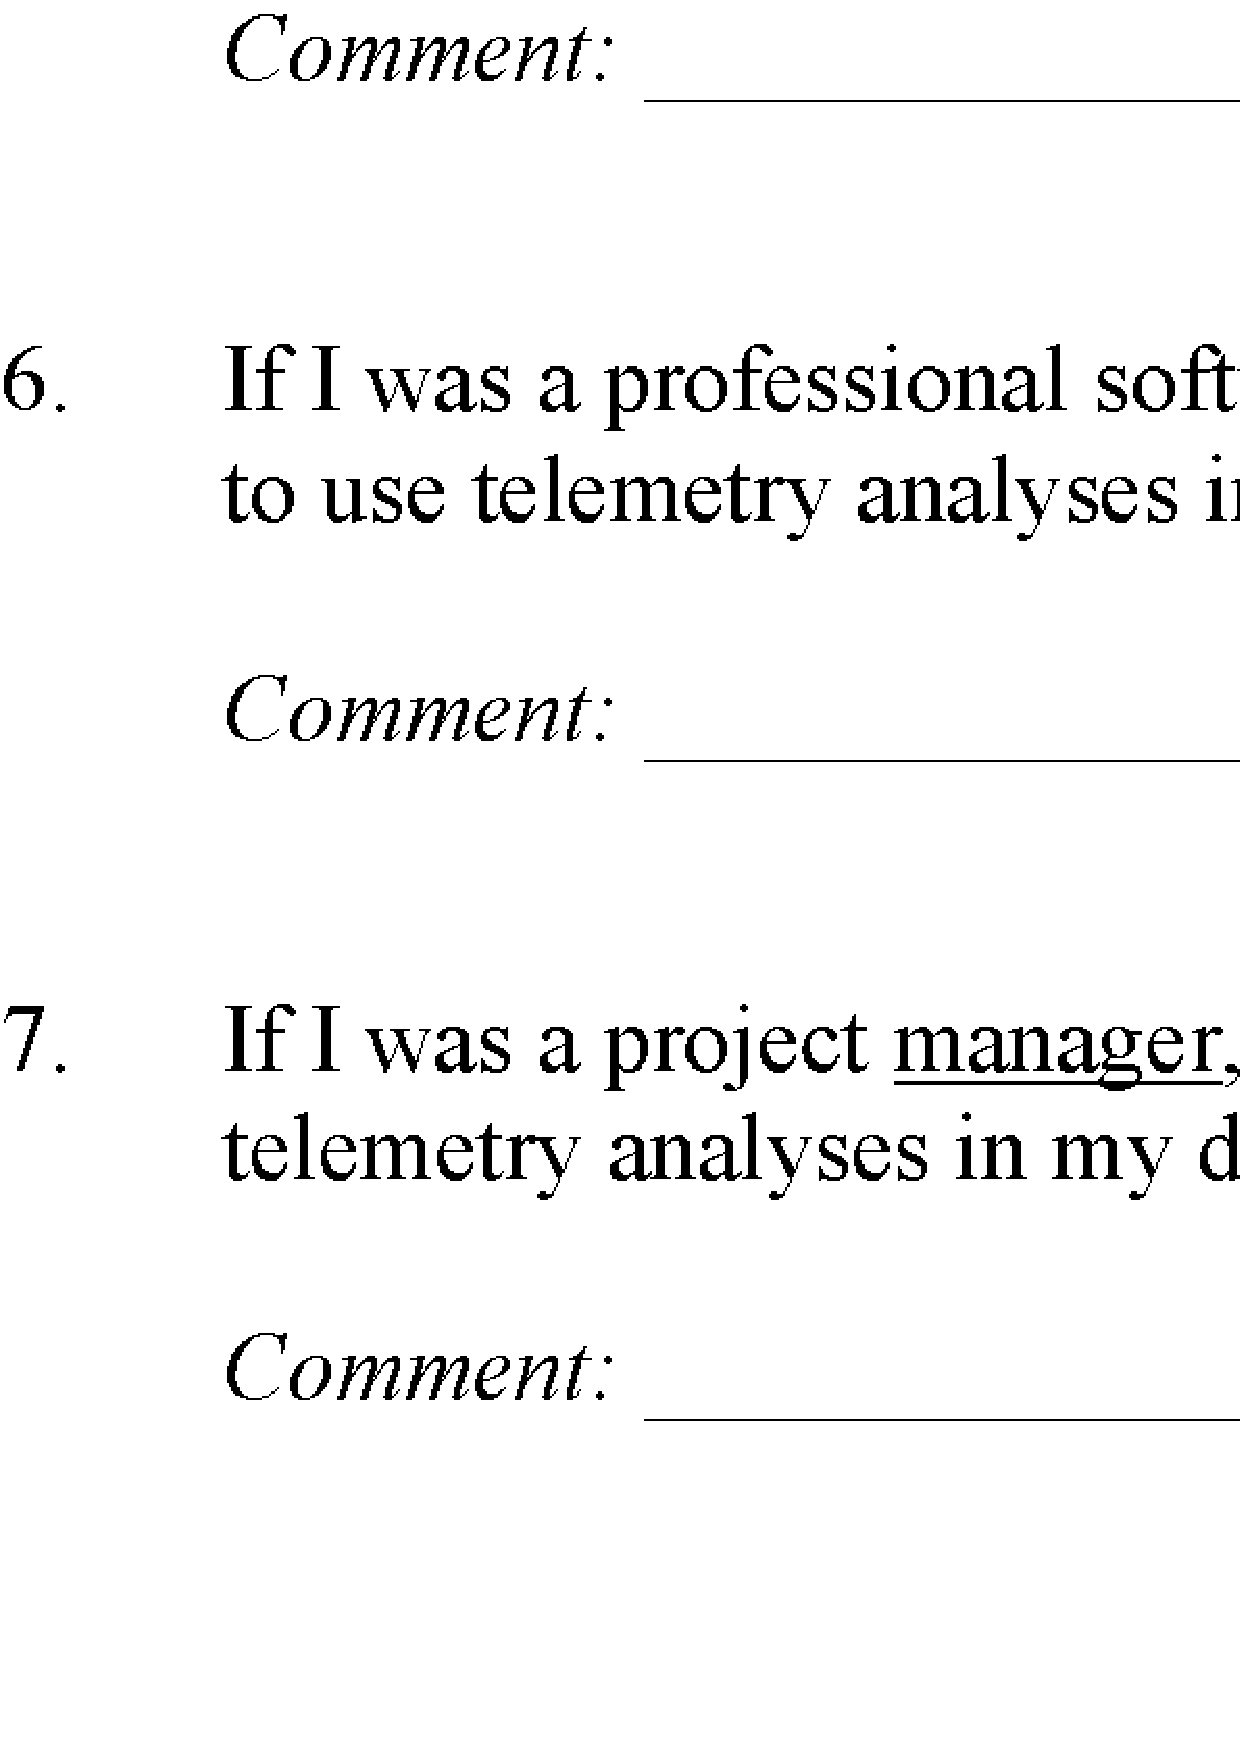
\includegraphics[height=1.00\textheight]{figures/ClassroomSurveyPage2}
\end{figure}
 
\begin{figure}[p]
  \includegraphics[height=1.00\textheight]{figures/ClassroomSurveyPage3}
\end{figure}

  \bibliographystyle{plain}
  \bibliography{reference/thesis}

\end{document}
